%===============================================================================
% LaTeX sjabloon voor de bachelorproef toegepaste informatica aan HOGENT
% Meer info op https://github.com/HoGentTIN/latex-hogent-report
%===============================================================================

\documentclass[dutch,dit,thesis]{hogentreport}


\usepackage[acronym]{glossaries}

\makeglossaries

\newacronym{iot}{IoT}{Internet-of-Things}
\newacronym{poc}{PoC}{Proof-of-Concept}
\newacronym{wgc}{WGC}{Wijkgezondheidscentrum}
\newacronym{pir}{PIR}{Passive Infrared}
\newacronym{ir}{IR}{Infrared}
\newacronym{rtsp}{RTSP}{Real-Time Streaming Protoco}


% TODO:
% - If necessary, replace the option `dit`' with your own department!
%   Valid entries are dbo, dbt, dgz, dit, dlo, dog, dsa, soa
% - If you write your thesis in English (remark: only possible after getting
%   explicit approval!), remove the option "dutch," or replace with "english".

\usepackage{lipsum} % For blind text, can be removed after adding actual content

%% Pictures to include in the text can be put in the graphics/ folder
\graphicspath{{../graphics/}}

%% For source code highlighting, requires pygments to be installed
%% Compile with the -shell-escape flag!
\usepackage[chapter]{minted}
%% If you compile with the make_thesis.{bat,sh} script, use the following
%% import instead:
%%\usepackage[chapter,outputdir=../output]{minted}
\usemintedstyle{solarized-light}

%% Formatting for minted environments.
\setminted{%
    autogobble,
    frame=lines,
    breaklines,
    linenos,
    tabsize=4
}

%% Ensure the list of listings is in the table of contents
\renewcommand\listoflistingscaption{%
    \IfLanguageName{dutch}{Lijst van codefragmenten}{List of listings}
}
\renewcommand\listingscaption{%
    \IfLanguageName{dutch}{Codefragment}{Listing}
}
\renewcommand*\listoflistings{%
    \cleardoublepage\phantomsection\addcontentsline{toc}{chapter}{\listoflistingscaption}%
    \listof{listing}{\listoflistingscaption}%
}

% Other packages not already included can be imported here

%%---------- Document metadata -------------------------------------------------
% TODO: Replace this with your own information
\author{Brahim Mahfoudhi}
\supervisor{Dhr. S. De Gheselle}
\cosupervisor{Dhr. L. Anciaux}
\title[]%
    {Validatie van een IoT-systeem voor realtime monitoring en voorspelling van wachtruimtebezetting: vergelijking met Google Occupancy Analytics}
\academicyear{\advance\year by -1 \the\year--\advance\year by 1 \the\year}
\examperiod{1}
\degreesought{\IfLanguageName{dutch}{Professionele bachelor in de toegepaste informatica}{Bachelor of applied computer science}}
\partialthesis{false} %% To display 'in partial fulfilment'
%\institution{Internshipcompany BVBA.}

%% Add global exceptions to the hyphenation here
\hyphenation{back-slash}

%% The bibliography (style and settings are  found in hogentthesis.cls)
\addbibresource{bachproef.bib}            %% Bibliography file
\addbibresource{../voorstel/voorstel.bib} %% Bibliography research proposal
\defbibheading{bibempty}{}

%% Prevent empty pages for right-handed chapter starts in twoside mode
\renewcommand{\cleardoublepage}{\clearpage}

\renewcommand{\arraystretch}{1.2}

%% Content starts here.
\begin{document}

%---------- Front matter -------------------------------------------------------

\frontmatter

\hypersetup{pageanchor=false} %% Disable page numbering references
%% Render a Dutch outer title page if the main language is English
\IfLanguageName{english}{%
    %% If necessary, information can be changed here
    \degreesought{Professionele Bachelor toegepaste informatica}%
    \begin{otherlanguage}{dutch}%
       \maketitle%
    \end{otherlanguage}%
}{}

%% Generates title page content
\maketitle
\hypersetup{pageanchor=true}

%%=============================================================================
%% Voorwoord
%%=============================================================================

\chapter*{\IfLanguageName{dutch}{Woord vooraf}{Preface}}%
\label{ch:voorwoord}
\TODO
%% TODO:
%% Het voorwoord is het enige deel van de bachelorproef waar je vanuit je
%% eigen standpunt (``ik-vorm'') mag schrijven. Je kan hier bv. motiveren
%% waarom jij het onderwerp wil bespreken.
%% Vergeet ook niet te bedanken wie je geholpen/gesteund/... heeft

%“Het implementeren van Internet of Things (IoT) om de wachttijden voor patiënten in de afdeling Accident and Emergency (A\&E) van de National Health Service (NHS) te verkorten”. Dit onderzoek werd geschreven met als doel om te bepalen of IoT een daadwerkelijke oplossing kan bieden tegen de langdurige wachttijden. Dit onderwerp heb ik gekozen samen met mijn mede-student Mohamed-Ali Kasraoui. Allereerst wil ik hem bedanken voor zijn waardevolle bijdrage, zonder welke dit onderzoek niet had kunnen plaatsvinden.

%De keuze voor het onderwerp werd sterk beïnvloed door de langdurige ziekte die ik aan het begin van mijn studies doormaakte. Het zijn voor mij zeer moeilijke jaren geweest, voor die reden was het van uiterst belang dat dit onderzoek zich op de medische sector richt. Het was voor mij van groot belang dat het onderzoek dat ik uitvoerde een waardevolle bijdrage zou leveren aan de medische wereld, waarvoor ik zeer dankbaar ben. %%TODO: ERVARING TIJDENS BACHELORPROEF

%%TODO: Bedanking Lectoren, Promotor, co-promotor
%Ik wil iedere lector bedanken in deze drie geweldige jaren, ik heb dankzij voldoende 


%Ik wens u veel leesplezier toe.

%Brahim Mahfoudhi





%%=============================================================================
%% Samenvatting
%%=============================================================================

% TODO: De "abstract" of samenvatting is een kernachtige (~ 1 blz. voor een
% thesis) synthese van het document.
%
% Een goede abstract biedt een kernachtig antwoord op volgende vragen:
%
% 1. Waarover gaat de bachelorproef?
% 2. Waarom heb je er over geschreven?
% 3. Hoe heb je het onderzoek uitgevoerd?
% 4. Wat waren de resultaten? Wat blijkt uit je onderzoek?
% 5. Wat betekenen je resultaten? Wat is de relevantie voor het werkveld?
%
% Daarom bestaat een abstract uit volgende componenten:
%
% - inleiding + kaderen thema
% - probleemstelling
% - (centrale) onderzoeksvraag
% - onderzoeksdoelstelling
% - methodologie
% - resultaten (beperk tot de belangrijkste, relevant voor de onderzoeksvraag)
% - conclusies, aanbevelingen, beperkingen
%
% LET OP! Een samenvatting is GEEN voorwoord!

%%---------- Nederlandse samenvatting -----------------------------------------
%
% TODO: Als je je bachelorproef in het Engels schrijft, moet je eerst een
% Nederlandse samenvatting invoegen. Haal daarvoor onderstaande code uit
% commentaar.
% Wie zijn bachelorproef in het Nederlands schrijft, kan dit negeren, de inhoud
% wordt niet in het document ingevoegd.

\IfLanguageName{english}{%
\selectlanguage{dutch}
\chapter*{Samenvatting}
\lipsum[1-4]
\selectlanguage{english}
}{}

%%---------- Samenvatting -----------------------------------------------------
% De samenvatting in de hoofdtaal van het document

\chapter*{\IfLanguageName{dutch}{Samenvatting}{Abstract}}

De wachttijden bij dienstverlenende organisaties zorgen al jarenlang voor frustratie bij cliënten. Ondanks interne optimalisaties en digitalisering blijft het voor veel leden moeilijk om vlot geholpen te worden zonder lange wachttijden, vooral tijdens piekuren. Dit leidt tot onnodige frustraties en het gevoel dat men onvoldoende gehoord wordt. Om die reden richt dit onderzoek zich op het beantwoorden van de volgende vraag: Hoe kan IoT-technologie worden ingezet om de bezettingsgraad van wachtruimtes in real-time te meten en voorspellende analyses toe te passen, met als doel het inzicht in wachttijden en de efficiëntie van bezoekersbeheer te verbeteren? \\

Naast het verbeteren van bezoekersstromen en wachttijdbeheer kan het systeem ook waardevolle input leveren voor bredere optimalisatiedoeleinden, zoals triageprocessen, personeelsplanning en capaciteitsbeheer, zeker in sectoren waar seizoensinvloeden een rol spelen. \\

Het onderzoek start met een analyse van de uitgevoerde literatuurstudie over de bestaande oplossingen. Vervolgens worden de in de literatuur geïdentificeerde IoT-apparaten geanalyseerd en wordt hieruit een selectie gemaakt. De devices worden uiteindelijk met elkaar vergeleken om de meest geschikte devices voor de proof-of-concept te selecteren. De proof-of-concept bestaat uit drie fasen. Eerst wordt een nulmeting uitgevoerd met behulp van Google Vertex AI Occupancy Analytics. Vervolgens wordt een IoT-gebaseerd Real-Time Bezettingsmonitoring Systeem geïmplementeerd. Tot slot vindt een evaluatie plaats waarbij de gegevens van zowel de Google Vertex AI Occupancy Analytics als het IoT-gebaseerde Real-Time Bezettingsmonitoring Systeem met elkaar worden vergeleken. \\
%TODO de werkelijke resultaten toevoegen samen met de Aanbevelingen op basis van je resultaten Beperkingen van het onderzoek NADAT DE ONDERZOEK AFGEROND IS

De resultaten zullen aantonen in welke mate IoT-technologie in staat is om nauwkeurige en real-time informatie te leveren over de bezettingsgraad van wachtruimtes. Daarnaast geven ze inzicht in hoe het IoT-gebaseerde systeem zich verhoudt tot het op beeldherkenning gebaseerde systeem van Google Occupancy Analytics.

%\lipsum[1-4]


%---------- Inhoud, lijst figuren, ... -----------------------------------------

\tableofcontents

% In a list of figures, the complete caption will be included. To prevent this,
% ALWAYS add a short description in the caption!
%
%  \caption[short description]{elaborate description}
%
% If you do, only the short description will be used in the list of figures

\listoffigures


% If you included tables and/or source code listings, uncomment the appropriate
% lines.
\listoftables


\listoflistings
\begin{listing}[H]
    \caption{SQL-query om de relevante tellingen per minuut te extraheren}
    \label{lst:tellingen}
    \begin{minted}[fontsize=\footnotesize, breaklines=true]{sql}
        WITH per_second_counts AS (
        SELECT
        TIMESTAMP_TRUNC(
        TIMESTAMP(SUBSTR(JSON_VALUE(annotation, "$.currentTime"), 1, 26)), SECOND
        ) AS ts,
        CAST(JSON_VALUE(count_obj, "$.count") AS INT64) AS people_in_zone
        FROM
        `reolink-occupancy-project.occupancy_dataset.occupancy_dataset_table`,
        UNNEST(JSON_EXTRACT_ARRAY(annotation, "$.stats.activeZoneCounts")) AS zone,
        UNNEST(JSON_EXTRACT_ARRAY(zone, "$.counts")) AS count_obj
        WHERE
        JSON_VALUE(zone, "$.annotation.displayName") = "wgc"
        AND JSON_VALUE(count_obj, "$.entity.labelString") = "Person"
        AND TIMESTAMP(SUBSTR(JSON_VALUE(annotation, "$.currentTime"), 1, 26)) >= TIMESTAMP("2025-07-15")
        ),
        with_flags AS (
        SELECT
        TIMESTAMP_TRUNC(ts, MINUTE) AS minute,
        people_in_zone,
        IF(people_in_zone > 0, 1, 0) AS is_present
        FROM per_second_counts
        ),
        grouped_stats AS (
        SELECT
        minute,
        COUNTIF(is_present = 1) AS seconds_present,
        AVG(people_in_zone) AS avg_people,
        MAX(people_in_zone) AS max_people
        FROM with_flags
        GROUP BY minute
        )
        SELECT
        minute,
        seconds_present,
        avg_people,
        max_people,
        CASE 
        WHEN seconds_present >= 10 THEN 'Geldig (>=10s aanwezig)'
        ELSE 'Kort (<10s aanwezig)'
        END AS status
        FROM grouped_stats
        WHERE seconds_present >= 10
        ORDER BY minute;
    \end{minted}
\end{listing}

\begin{listing}[H]
    \caption{Voorspellingsmodel op basis van ARIMA\_PLUS}
    \label{lst:people_forecast_model}
    \begin{minted}[fontsize=\footnotesize, breaklines=true]{sql}
        CREATE OR REPLACE MODEL `reolink-occupancy-project.occupancy_dataset.occupancy_arima`
        OPTIONS(
        model_type='ARIMA_PLUS',
        time_series_timestamp_col='minute',
        time_series_data_col='avg_people',
        horizon=1440,  -- aantal minuten vooruit (24h * 60min)
        time_series_id_col=NULL
        ) AS
        SELECT
        minute,
        avg_people
        FROM (
        WITH per_second_counts AS (
        SELECT
        TIMESTAMP_TRUNC(
        TIMESTAMP(SUBSTR(JSON_VALUE(annotation, "$.currentTime"), 1, 26)), SECOND
        ) AS ts,
        CAST(JSON_VALUE(count_obj, "$.count") AS INT64) AS people_in_zone
        FROM
        `reolink-occupancy-project.occupancy_dataset.occupancy_dataset_table`,
        UNNEST(JSON_EXTRACT_ARRAY(annotation, "$.stats.activeZoneCounts")) AS zone,
        UNNEST(JSON_EXTRACT_ARRAY(zone, "$.counts")) AS count_obj
        WHERE
        JSON_VALUE(zone, "$.annotation.displayName") = "wgc"
        AND JSON_VALUE(count_obj, "$.entity.labelString") = "Person"
        AND TIMESTAMP(SUBSTR(JSON_VALUE(annotation, "$.currentTime"), 1, 26)) >= TIMESTAMP("2025-07-15")
        ),
        with_flags AS (
        SELECT
        TIMESTAMP_TRUNC(ts, MINUTE) AS minute,
        people_in_zone,
        IF(people_in_zone > 0, 1, 0) AS is_present
        FROM per_second_counts
        ),
        grouped_stats AS (
        SELECT
        minute,
        COUNTIF(is_present = 1) AS seconds_present,
        AVG(people_in_zone) AS avg_people,
        MAX(people_in_zone) AS max_people
        FROM with_flags
        GROUP BY minute
        )
        SELECT
        minute,
        avg_people
        FROM grouped_stats
        WHERE seconds_present >= 10
        );
    \end{minted}
\end{listing}

\begin{listing}[H]
    \caption{Forecast ophalen uit het ARIMA\_PLUS model}
    \label{lst:people_forecast_query}
    \begin{minted}[fontsize=\small, breaklines=true]{sql}
        SELECT
        *
        FROM
        ML.FORECAST(MODEL `reolink-occupancy-project.occupancy_dataset.occupancy_arima`,
        STRUCT(1440 AS horizon));
    \end{minted}
\end{listing}


\begin{listing}[H]
    \caption{Berekening van per-minute statistieken van aanwezige personen}
    \label{lst:people_per_minute}
    \small
    \begin{minted}[breaklines=true]{sql}
        WITH per_second_counts AS (
        SELECT
        TIMESTAMP_TRUNC(
        TIMESTAMP(SUBSTR(JSON_VALUE(annotation, "$.currentTime"), 1, 26)), SECOND
        ) AS ts,
        CAST(JSON_VALUE(count_obj, "$.count") AS INT64) AS people_in_zone
        FROM `reolink-occupancy-project.occupancy_dataset.occupancy_dataset_table`,
        UNNEST(JSON_EXTRACT_ARRAY(annotation, "$.stats.activeZoneCounts")) AS zone,
        UNNEST(JSON_EXTRACT_ARRAY(zone, "$.counts")) AS count_obj
        WHERE JSON_VALUE(zone, "$.annotation.displayName") = "wgc"
        AND JSON_VALUE(count_obj, "$.entity.labelString") = "Person"
        AND TIMESTAMP(SUBSTR(JSON_VALUE(annotation, "$.currentTime"), 1, 26)) >= TIMESTAMP("2025-07-15")
        ),
        with_flags AS (
        SELECT
        TIMESTAMP_TRUNC(ts, MINUTE) AS minute,
        people_in_zone,
        IF(people_in_zone > 0, 1, 0) AS is_present
        FROM per_second_counts
        ),
        grouped_stats AS (
        SELECT
        minute,
        COUNTIF(is_present = 1) AS seconds_present,
        AVG(people_in_zone) AS avg_people
        FROM with_flags
        GROUP BY minute
        HAVING COUNTIF(is_present = 1) >= 10
        )
    \end{minted}
\end{listing}

\begin{listing}[H]
    \caption{Forecast en MAPE berekening}
    \label{lst:people_forecast_mape}
    \small
    \begin{minted}[breaklines=true]{sql}
        forecast_hourly AS (
        SELECT
        forecast_timestamp AS ts_hour,
        GREATEST(forecast_value, 0) AS yhat
        FROM ML.FORECAST(
        MODEL `reolink-occupancy-project.occupancy_dataset.people_forecast_model`,
        STRUCT(80 AS horizon)
        )
        ),
        forecast_minute AS (
        SELECT
        TIMESTAMP_ADD(f1.ts_hour, INTERVAL m MINUTE) AS ts,
        f1.yhat + (f2.yhat - f1.yhat) * m / 60.0 AS yhat
        FROM forecast_hourly f1
        JOIN forecast_hourly f2
        ON f2.ts_hour = TIMESTAMP_ADD(f1.ts_hour, INTERVAL 1 HOUR)
        CROSS JOIN UNNEST(GENERATE_ARRAY(0, 59)) AS m
        )
        SELECT
        ROUND(AVG(ABS(SAFE_DIVIDE(f.yhat - o.avg_people, o.avg_people))) * 100, 2) AS MAPE_percent,
        COUNT(*) AS matched_rows
        FROM forecast_minute f
        JOIN grouped_stats o
        ON f.ts = o.minute
        WHERE o.avg_people > 0;
    \end{minted}
\end{listing}

   
\begin{listing}[H]
    \caption{Deel 1 – Setup en Configuratie van de ESP32}
    \label{lst:esp32_setup}
    \begin{minted}[fontsize=\footnotesize, breaklines=true]{cpp}
        #include <WiFi.h>
        #include <InfluxDbClient.h>
        
        const char* ssid = "YOUR_SSID";
        const char* password = "YOUR_PASSWORD";
        
        #define INFLUXDB_URL "http://YOUR_URL:8086"
        #define INFLUXDB_TOKEN "YOUR_TOKEN"
        #define INFLUXDB_ORG "YOUR_ORG"
        #define INFLUXDB_BUCKET "sensor_data"
        
        InfluxDBClient client(INFLUXDB_URL, INFLUXDB_ORG, INFLUXDB_BUCKET, INFLUXDB_TOKEN);
        Point people("people_counter");
        
        const int sensorIn = 14;
        const int sensorOut = 25; 
       
        enum State { IDLE, SENSOR_IN_TRIGGERED, SENSOR_OUT_TRIGGERED };
        State state = IDLE;
        
        int peopleCount = 0;
        int enteredLastMinute = 0;
        int exitedLastMinute = 0;
        unsigned long lastSendTime = 0;
        unsigned long stateStartTime = 0;
        
        void setup() {
            Serial.begin(115200);
            pinMode(sensorIn, INPUT_PULLUP);
            pinMode(sensorOut, INPUT_PULLUP);
            
            WiFi.begin(ssid, password);
            while (WiFi.status() != WL_CONNECTED) {
                delay(500);
                Serial.print(".");
            }
            Serial.println("\nWiFi connected");
            
            if (client.validateConnection()) {
                Serial.println("Connected to InfluxDB!");
            } else {
                Serial.print("InfluxDB connection failed: ");
                Serial.println(client.getLastErrorMessage());
            }
            
            people.addTag("location", "wachtzaal");
            people.addTag("device", "esp32_deur_sensor");
        }
    \end{minted}
\end{listing}


\begin{listing}[H]
    \caption{Deel 2 – Sensorlogica en hoofdloop}
    \label{lst:esp32_loop}
    \begin{minted}[fontsize=\footnotesize, breaklines=true]{cpp}
        void loop() {
            if (WiFi.status() != WL_CONNECTED) {
                WiFi.reconnect();
                delay(5000);
            }
            
            bool inBroken = isStableLow(sensorIn);
            bool outBroken = isStableLow(sensorOut);
            
            switch (state) {
                case IDLE:
                if (inBroken) {
                    state = SENSOR_IN_TRIGGERED;
                    stateStartTime = millis();
                } else if (outBroken) {
                    state = SENSOR_OUT_TRIGGERED;
                    stateStartTime = millis();
                }
                break;
                case SENSOR_IN_TRIGGERED:
                if (outBroken) {
                    peopleCount++;
                    enteredLastMinute++;
                    while (digitalRead(sensorOut) == LOW) delay(10);
                    state = IDLE;
                } else if (millis() - stateStartTime > 3000) {
                    state = IDLE;
                }
                break;
                case SENSOR_OUT_TRIGGERED:
                if (inBroken) {
                    if (peopleCount > 0) peopleCount--;
                    exitedLastMinute++;
                    while (digitalRead(sensorIn) == LOW) delay(10);
                    state = IDLE;
                } else if (millis() - stateStartTime > 3000) {
                    state = IDLE;
                }
                break;
            }
            
            if (millis() - lastSendTime > 60000) {
                sendToInfluxDB();
                enteredLastMinute = 0;
                exitedLastMinute = 0;
                lastSendTime = millis();
            }
            
            delay(5);
        }
    \end{minted}
\end{listing}

\begin{listing}[H]
    \caption{Deel 3 – Hulpfuncties voor sensorstabiliteit en data-upload}
    \label{lst:esp32_utils}
    \begin{minted}[fontsize=\footnotesize, breaklines=true]{cpp}
        bool isStableLow(int pin, unsigned long duration = 30) {
            unsigned long start = millis();
            while (millis() - start < duration) {
                if (digitalRead(pin) != LOW) return false;
                delay(5);
            }
            return true;
        }
        
        void sendToInfluxDB() {
            if (WiFi.status() != WL_CONNECTED) {
                Serial.println("Wi-Fi niet verbonden. Kan niet verzenden.");
                return;
            }
            
            people.clearFields();
            people.addField("count", peopleCount);
            people.addField("entered", enteredLastMinute);
            people.addField("exited", exitedLastMinute);
            
            if (!client.writePoint(people)) {
                Serial.print("Fout bij verzenden naar InfluxDB: ");
                Serial.println(client.getLastErrorMessage());
            } else {
                Serial.println("Gegevens succesvol verzonden naar InfluxDB.");
            }
        }
    \end{minted}
\end{listing}

\begin{listing}[H]
    \caption{Vergelijking van IoT- en WGC-data per minuut-van-de-dag in Python}
    \label{lst:python-iot-wgc}
    \begin{minted}[linenos,fontsize=\small,breaklines]{python}
        import pandas as pd
        
        iot = pd.read_excel("iot_data.xlsx")
        wgc = pd.read_excel("wgc-data-dinsdag.xlsx")
        
        iot["minute"] = pd.to_datetime(iot["minute"]).dt.tz_localize("Europe/Brussels")
        .dt.floor("min")
        wgc["minute"] = pd.to_datetime(wgc["minute"]).dt.tz_localize("Europe/Brussels")
        .dt.floor("min")
        
        iot["minute_of_day"] = iot["minute"].dt.hour * 60 + iot["minute"].dt.minute
        wgc["minute_of_day"] = wgc["minute"].dt.hour * 60 + wgc["minute"].dt.minute
        
        iot_avg = iot.groupby("minute_of_day")["count"].mean()
        wgc_avg = wgc.groupby("minute_of_day")["avg_people"].mean()
        
        comp = pd.concat([iot_avg, wgc_avg], axis=1).dropna().reset_index()
        comp["hhmm"] = comp["minute_of_day"].apply(lambda m: f"{m//60:02d}:{m%60:02d}")
        
        comp.to_excel("vergelijking_dinsdag_op_tijdvandag.xlsx", index=False)
    \end{minted}
\end{listing}

\begin{listing}[H]
    \caption{Visualisatie en vergelijking van IoT- en WGC-data met Python}
    \label{lst:python-iot-wgc-plot}
    \begin{minted}[linenos,fontsize=\scriptsize,breaklines]{python}
        import matplotlib.pyplot as plt
        import matplotlib.ticker as ticker
        import pandas as pd
        
        df = pd.read_excel("vergelijking_dinsdag_op_tijdvandag.xlsx")
        
        df["difference"] = df["iot_avg_people"] - df["wgc_avg_people"]
        
        mean_iot = df["iot_avg_people"].mean()
        mean_wgc = df["wgc_avg_people"].mean()
        mean_diff = df["difference"].mean()
        corr = df["iot_avg_people"].corr(df["wgc_avg_people"])
        
        def plot_with_reduced_xticks(x, y_list, labels, colors, xlabel, ylabel, title, figsize=(12,6)):
        plt.figure(figsize=figsize)
        for y, label, color in zip(y_list, labels, colors):
        plt.plot(x, y, label=label, color=color)
        
        ax = plt.gca()
        ax.xaxis.set_major_locator(ticker.MaxNLocator(nbins=10))  # maximaal 10 labels
        plt.xticks(rotation=45)
        plt.xlabel(xlabel)
        plt.ylabel(ylabel)
        plt.title(title)
        plt.legend()
        plt.tight_layout()
        plt.show()
        
        plot_with_reduced_xticks(
        x=df["hhmm"],
        y_list=[df["iot_avg_people"], df["wgc_avg_people"]],
        labels=["IoT-systeem", "Google Vertex AI (WGC)"],
        colors=["blue", "orange"],
        xlabel="Tijd (HH:MM)",
        ylabel="Gemiddeld aantal personen",
        title="Vergelijking bezettingsgraad IoT-systeem vs Google Vertex AI"
        )
        
        plot_with_reduced_xticks(
        x=df["hhmm"],
        y_list=[df["difference"]],
        labels=["Verschil (IoT - WGC)"],
        colors=["red"],
        xlabel="Tijd (HH:MM)",
        ylabel="Verschil in personen",
        title="Verschil in metingen per minuut",
        figsize=(12,4)
        )
        
        mean_iot, mean_wgc, mean_diff, corr
    \end{minted}
\end{listing}


% Als je een lijst van afkortingen of termen wil toevoegen, dan hoort die
% hier thuis. Gebruik bijvoorbeeld de ``glossaries'' package.
% https://www.overleaf.com/learn/latex/Glossaries


%---------- Kern ---------------------------------------------------------------

\mainmatter{}

% De eerste hoofdstukken van een bachelorproef zijn meestal een inleiding op
% het onderwerp, literatuurstudie en verantwoording methodologie.
% Aarzel niet om een meer beschrijvende titel aan deze hoofdstukken te geven of
% om bijvoorbeeld de inleiding en/of stand van zaken over meerdere hoofdstukken
% te verspreiden!

%%=============================================================================
%% Inleiding
%%=============================================================================

\chapter{\IfLanguageName{dutch}{Inleiding}{Introduction}}%
\label{ch:inleiding}

%De inleiding moet de lezer net genoeg informatie verschaffen om het onderwerp te begrijpen en in te zien waarom de onderzoeksvraag de moeite waard is om te onderzoeken. In de inleiding ga je literatuurverwijzingen beperken, zodat de tekst vlot leesbaar blijft. Je kan de inleiding verder onderverdelen in secties als dit de tekst verduidelijkt. Zaken die aan bod kunnen komen in de inleiding~\autocite{Pollefliet2011}:

\begin{itemize}
  \item context, achtergrond
  \item afbakenen van het onderwerp
  \item verantwoording van het onderwerp, methodologie
  \item probleemstelling
  \item onderzoeksdoelstelling
  \item onderzoeksvraag
  \item \ldots
\end{itemize}

\section{\IfLanguageName{dutch}{Probleemstelling}{Problem Statement}}%
\label{sec:probleemstelling}
Volgens de bevindingen uit het onderzoek zitten de Accident and Emergency (A\&E) afdelingen van de National Health Service (NHS) in een “vreselijke staat”. De studie toont namelijk aan dat meer dan 100.000 kinderen vorig jaar boven de 6 uur moesten wachten en dat bijna 10 procent van alle patiënten nu 12 uur of langer moet wachten om behandeld te worden \autocite{LordDarzi2024}. Deze langdurige wachttijden hebben serieuze consequenties voor patiënten. Volgens een toespraak over het onderzoek door de Britse Premier, Sir Keir Starmer, zijn de lange A\&E wachttijden niet alleen een bron van angst en bezorgdheid, maar leiden ook tot duizenden vermijdbare sterfgevallen. Volgens de Royal College of Emergency Medicine gaat het om 14.000 extra sterfgevallen per jaar \autocite{Starmer2024}.


%Uit je probleemstelling moet duidelijk zijn dat je onderzoek een meerwaarde heeft voor een concrete doelgroep. De doelgroep moet goed gedefinieerd en afgelijnd zijn. Doelgroepen als ``bedrijven,'' ``KMO's'', systeembeheerders, enz.~zijn nog te vaag. Als je een lijstje kan maken van de personen/organisaties die een meerwaarde zullen vinden in deze bachelorproef (dit is eigenlijk je steekproefkader), dan is dat een indicatie dat de doelgroep goed gedefinieerd is. Dit kan een enkel bedrijf zijn of zelfs één persoon (je co-promotor/opdrachtgever).

\section{Doel van het onderzoek}
Om een oplossing te vinden voor dit langdurige probleem richt dit onderzoek zich op het uitzoeken of Internet of Things (IoT) een daadwerkelijke oplossing kan zijn om de lange wachttijden op de spoedafdelingen wereldwijd te verkorten. Deze studie zal verkennen wat de oorzaak is van de lange wachttijden door een oorzakenanalyse uit te voeren en gegevens te verzamelen van een ziekenhuis in Vlaanderen. De inzichten uit dit onderzoek kunnen niet alleen bijdragen aan verbeteringen binnen Vlaanderen, maar ook waardevolle lessen bieden voor ziekenhuizen in andere landen.

\section{\IfLanguageName{dutch}{Onderzoeksvraag}{Research question}}%
\label{sec:onderzoeksvraag}
De centrale onderzoeksvraag in dit onderzoek luidt: "Kunnen Internet of Things (IoT)-\-technologieën worden toegepast om wachttijden op de A\&E-afdelingen te verminderen?" Om deze vraag te beantwoorden, is het belangrijk om een antwoord te geven op een aantal deelvragen in het probleem- en oplossingsdomein. 

Probleem domein:
\begin{itemize}
    \item Wat zijn de belangrijkste oorzaken van lange wachttijden op A\&E-afdelingen?
    \item Hoe kan de "5 Whys"-methode helpen om de onderliggende oorzaak van wachttijden te identificeren?
    \item Welke aanpassingen in de wachtruimte kunnen de wachttijden verkorten?
    \item Hoe kan worden aangetoond dat IoT de wachttijd kan verkorten?
\end{itemize}


Oplossing domein:
\begin{itemize}
    \item Welke IoT-apparaten kunnen bijdragen aan het verminderen van wachttijden?
    \item Hoe kunnen bestaande casestudies gebruikt worden om IoT-technologieën te identificeren voor wachttijd vermindering in A\&E-afdelingen?
    \item Welke criteria worden gebruikt in de vergelijkende analyse van IoT-apparaten om het meest geschikte apparaat te selecteren voor de PoC?
    \item Hoe kunnen verschillende sensoren (zoals bewegingssensoren, aanwezigheidssensoren, lichtsluis- en infraroodsensoren, druksensoren en thermische camera’s) anoniem real-time data verzamelen om wachttijden in A\&E-afdelingen te verkorten, zonder persoonlijke gegevens te verwerken?
    \item Welke plaatsingsstrategieën zijn het meest effectief voor het verzamelen van deze data?
    % \item Hoe kan een dashboard real-time wachttijden en patiëntenvolgorde visualiseren om efficiëntie te verbeteren?
    \item Hoe wordt de PoC uitgevoerd met behulp van een centrale eenheid, sensor controller en sensoren om een Real-Time Smart Queue Management systeem \autocite{Ghazal2015} te implementeren zoals? 
    \item Hoe kan het scherm in de wachtruimte worden geïntegreerd met het cloudgebaseerde platform om de patiënten in real-time te informeren over hun wachttijd en positie in de wachtrij? \TODO
\end{itemize}

%Wees zo concreet mogelijk bij het formuleren van je onderzoeksvraag. Een onderzoeksvraag is trouwens iets waar nog niemand op dit moment een antwoord heeft (voor zover je kan nagaan). Het opzoeken van bestaande informatie (bv. ``welke tools bestaan er voor deze toepassing?'') is dus geen onderzoeksvraag. Je kan de onderzoeksvraag verder specifiëren in deelvragen. Bv.~als je onderzoek gaat over performantiemetingen, dan 

\section{\IfLanguageName{dutch}{Onderzoeksdoelstelling}{Research objective}}%
\label{sec:onderzoeksdoelstelling}
Het is van cruciaal belang om dit onderwerp te onderzoeken vanwege de potentiële impact op de gezondheidszorg en het welzijn van A\&E patiënten. De onderzoeksdoelstelling is om te bepalen of IoT een werkelijke oplossing kan bieden voor de lange A\&E wachttijden.


\section{Verwachte eindresultaat} 
Het verwachte eindresultaat van dit onderzoek is dat de verschillende deelvragen beantwoord zijn, verder wordt er verwacht dat de proof-of-concept een duidelijk antwoord biedt op de onderzoeksvraag. De resultaten zullen vervolgens gebruikt worden om aanbevelingen te formuleren voor de implementatie van IoT-oplossingen binnen de A\&E afdelingen, met als doel de wachttijden te verminderen.

%Wat is het beoogde resultaat van je bachelorproef? Wat zijn de criteria voor succes? Beschrijf die zo concreet mogelijk. Gaat het bv.\ om een proof-of-concept, een prototype, een verslag met aanbevelingen, een vergelijkende studie, enz.

\section{\IfLanguageName{dutch}{Opzet van deze bachelorproef}{Structure of this bachelor thesis}}%
\label{sec:opzet-bachelorproef}

% Het is gebruikelijk aan het einde van de inleiding een overzicht te
% geven van de opbouw van de rest van de tekst. Deze sectie bevat al een aanzet
% die je kan aanvullen/aanpassen in functie van je eigen tekst.

De rest van deze bachelorproef is als volgt opgebouwd:

In Hoofdstuk~\ref{ch:stand-van-zaken} wordt een overzicht gegeven van de stand van zaken binnen het onderzoeksdomein, op basis van een literatuurstudie.

In Hoofdstuk~\ref{ch:methodologie} wordt de methodologie toegelicht en worden de gebruikte onderzoekstechnieken besproken om een antwoord te kunnen formuleren op de onderzoeksvragen.

% TODO: Vul hier aan voor je eigen hoofstukken, één of twee zinnen per hoofdstuk

In Hoofdstuk~\ref{ch:conclusie}, tenslotte, wordt de conclusie gegeven en een antwoord geformuleerd op de onderzoeksvragen. Daarbij wordt ook een aanzet gegeven voor toekomstig onderzoek binnen dit domein.
\usepackage{graphicx}
\usepackage{array}
\usepackage{longtable}
\usepackage{booktabs}
\usepackage{tabularx}
\usepackage[a4paper,margin=1in]{geometry}

%Engeland,
%Australië, Stockholm, Schotland en Noord-Ierland

\chapter{\IfLanguageName{dutch}{Stand van zaken}{State of the art}}%
\label{ch:stand-van-zaken}

\section{Inleiding}
Internet of Things is over de laatste twintig jaar enorm geëvolueerd, en het gebruik hiervan is wijdverspreid, van boeren in de agrarische sector tot artsen in de gezondheidszorg maken direct en indirect gebruik van IoT. Tegenwoordig worden miljarden van deze apparaten gebruikt door mensen om een verschil te maken in hun respectieve vakgebied. Ook in de gezondheidszorg biedt IoT veel mogelijkheden bij het aanpakken van grote problemen zoals de lange wachttijden in A\&E afdelingen.Diverse landen worden met dit probleem geconfronteerd, zoals Engeland, Australië, Zweden, Schotland en Noord-Ierland \autocite{Friebel2020}. Ook België krijgt hiermee te maken,  volgens een onderzoek uitgevoerd door \TODO Testaankoop wordt geconcludeerd dat Belgische ziekenhuizen wachttijdsproblemen ondervinden, maar dat deze variëren tussen ziekenhuizen. Deze langdurige wachttijden zorgen ervoor dat patiënten in sommige gevallen buitensporige wachttijden ervaren, in enkele gevallen moeten patiënten zelf over de twaalf-uur wachten voor behandelingen. Deze overmatige wachttijden hebben serieuze implicaties en kan in sommige gevallen leiden tot het overlijden van patiënten. Het gebruik van IoT devices biedt hiervoor een mogelijke oplossing om de langdurige wachttijden te verkorten door gebruik te maken van gegevensverzameling en automatisering. Dit hoofdstuk verkent de literatuur om een beter begrip te krijgen over IoT, de werking ervan en hoe het kan gebruikt worden om wachttijden te verminderen. Het hoofdstuk begint met een overzicht over IoT, het ontstaan en de betekenis ervan besproken worden. Verder worden de verschillende componenten van IoT behandeld en in detail wordt uitgewerkt. Vervolgens wordt IoT in de gezondheidszorg besproken waarbij de huidige implementaties hiervan volgens de literatuur worden opgesomd. Hierna komen de voor- en nadelen van IoT in de gezondheidszorg aan bod, gevolgd door een analyse van de beveiligings- en ethische kwesties. Hierop volgt een sectie over de wachttijden in A\&E-afdelingen en de impact hiervan op de zorgkwaliteit. Tot slot wordt besproken hoe IoT kan bijdragen aan het verminderen van de wachttijden met enkele voorbeelden van implementaties uit de literatuur.

\section{Overzicht Internet of Things}
De term \textit{Internet of Things} is ontstaan in 1999, toen Kevin Ashton, een Britse technologiepionier, verschillende objecten probeerde te verbinden met het internet door gebruik te maken van RFID-tags \autocite{Bassi2013, Rejeb2023}. Het concept Internet of Things verwijst naar een netwerk waarin fysieke objecten ('things') via het internet met elkaar communiceren. Deze objecten zijn uitgerust met sensoren en actuatoren om gegevens te kunnen verzamelen, verwerken en delen, waardoor ze slim en interactief worden \autocite{Elksasy2023}. Het concept wordt uiteindelijk beschouwd als een manier waarop verschillende objecten hun aanwezigheid behouden om een samenhangend geheel te vormen voor iedereen, overal, op ieder moment, met ieder medium en ieder netwerk, zoals geïllustreerd in Figuur \ref{fig:Figuur9}. 

\begin{figure}[h]
    \centering
    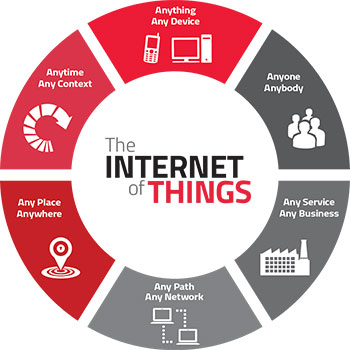
\includegraphics[width=0.4\textwidth]{img/bp/iot-concept.jpg}
    \caption{Internet of Things Networking}
    \label{fig:Figuur9}
    \textit{Source: \autocite{Dauwed2018}}
\end{figure}

Dankzij de voortdurende innovaties in de technologie hebben de laatste twee decennia een grote invloed gehad op de snelle vooruitgang van IoT. \autocite{Almutairi2024}. Hierdoor is het aantal aangesloten IoT devices sterk gestegen, met 7.74 miljard in 2019, 10.7 miljard in 2021 \autocite{Dawod2022} en tot 75 miljard in 2025 \autocite{Khan2019}. Sensoren, camera's en gelijkaardige apparaten worden al “geïntegreerd” in “woningen” en “voertuigen” \autocite{Dawod2022} en geïmplementeerd over verschillende sectoren zoals de “gezondheidszorg, landbouw, productie transport, milieu en nutsbedrijven \autocite{Naresh2020, Almutairi2024}. De implementatie van miljarden \autocite{Dawod2022} IoT devices over verschillende sectoren geeft een duidelijke representatie van de veranderingen die IoT zal brengen in de manier waarop men leeft, werkt en omgaat met de omgeving \autocite{Almutairi2024}. Dit deel heeft verschillende aspecten van IoT behandeld zoals de oorsprong, het concept en het gebruik. Het volgende deel zal dieper ingaan op de hardwarecomponenten om een beter begrip te verkrijgen in de werking van IoT.

%Deze technologie maakt het mogelijk om IoT in te zetten in verschillende sectoren, zoals transport, slimme steden, nutsbedrijven, milieu, gezondheidszorg en veiligheid. Volgens \autocite{Naresh2020} zal dit leiden tot 75 miljard verbonden IoT-devices in 2025 \autocite{Khan2019}. Dit benadrukt het belang van IoT als een technologie en het gebruik hiervan in diverse sectoren. Dit deel heeft verschillende aspecten van IoT behandeld zoals de oorsprong, het concept en het gebruik. Het volgende deel zal dieper ingaan op de hardwarecomponenten om een beter begrip te verkrijgen in de werking van IoT.

%De afgelopen twee decennia hebben een grote invloed gehad op de snelle vooruitgang van IoT \autocite{Almutairi2024}, hierdoor is het aantal aangesloten IoT devices sterk gestegen, met 7.74 miljard in 2019, 10.7 miljard in 2021 \autocite{Dawod2022} en 25.44 miljard tegen 2030 \autocite{Dawod2022}. Sensoren, camera's en gelijkaardige apparaten worden al “geïntegreerd” in “woningen” en “voertuigen” \autocite{Dawod2022} en geïmplementeerd over verschillende sectoren zoals de “gezondheidszorg, landbouw, productie” en slimme steden \autocite{Almutairi2024}.


%Zoals eerder aangetoond beschikt IoT over verschillende componenten die ervoor zorgen dat deze gegevens kan detecteren en verwerken. In het volgende deel worden deze componenten zorgvuldig geanalyseerd. 

\subsection{IoT hardware componenten} 
De IoT-omgeving bevat verschillende belangrijke componenten zoals sensoren, actuatoren, microprocessors, en communicatie protocollen. Deze componenten zorgen ervoor dat objecten slim worden en in staat zijn om met elkaar te communiceren \autocite{Abraham2023, Gharde2024}. In de volgende secties zullen de componenten in detail worden behandeld om een volledig begrip in de werking van IoT te krijgen. De eerste component dat geanalyseerd zal worden zijn de sensoren.

\subsubsection{Sensors}
Sensoren zijn een van de belangrijkste componenten in een IoT-structuur. De functie hiervan is het verzamelen van gegevens in een bepaalde omgeving \autocite{Abraham2023, Moyer2019}. Meer specifiek detecteren de sensoren elke “fysieke of chemische” verandering. Deze gegevens worden vervolgens verwerkt door de applicatie of device om slimme beslissingen te nemen en acties te automatiseren \autocite{Sehrawat2019}. Om een IoT-systeem compleet te maken, worden sensoren gebruikt in samenwerking met actuatoren. Deze worden in de volgende sectie besproken. Zie tabel \ref{tab:sensors} voor een weergave van een aantal IoT sensoren. Deze sensoren worden verder onderverdeeld in verschillende sub types zoals aangetoond door tabel \ref{tab:sensor_subtypes}.

\begin{table}[h]
    \raggedright
    \renewcommand{\arraystretch}{1.3}
    \small
    \caption{Sensor types en het gebruik ervan \autocite{Moyer2019, Sehrawat2019, Kumar2024, Balogun2017, Meenakshi2020, Tresanchez2018, Shanmugavalli2023, Gala2020, Gade2013, Chidurala2021, Karunarathne2018, Srinivasan2022}}
    \begin{tabular}{|c|m{4cm}|m{10cm}|}
        \hline
        \textbf{S/N} & \textbf{Sensor devices} & \textbf{Description} \\
        \hline
        1. & Motion sensor & Een bewegingsdetector is een IoT-device dat gebruikt wordt voor het detecteren van fysieke en dynamische bewegingen. Motion sensing kan ingezet worden om bijvoorbeeld een eigendom te beschermen door potentiële indringers te detecteren. In een onderzoek uitgevoerd door \autocite{Tiong2019} wordt motion sensing gebruikt als IoT-based Home Security System voor het detecteren van indringers. \\
        \hline
        2. & Pressure sensor & Een druksensor worden in IoT-systemen gebruikt om kracht en drukte te meten en detecteren. Deze sensor kan worden gebruikt om de aanwezigheid van gebruikers te monitoren op stoelen en bedden wat real-time informatie biedt\\
        \hline
        3. & Optical proximity sensor & Wordt gebruikt voor het detecteren van objecten door gebruik te maken van licht zonder fysieke contact. \\
        \hline
        4. & Wireless Communication & Is een belangrijk aspect van IoT, deze zorgt ervoor dat devices met elkaar kunnen communiceren door data te delen en verzenden. \\
        \hline
        5. & Thermal camera & Thermische camera's zijn sensoren die gebruikt worden om infrarode radiatie te detecteren van objecten met een temperatuur hoger dan nul graden. Deze sensoren kunnen gebruikt worden voor het monitoren van niet-intusieve bezetting \\
        \hline
        %4. & Magnetometers & Een magnetometer wordt gebruikt om magnetische velden te detecteren. In een studie uitgevoerd door \autocite{Hutagalung2021} worden magnetometers gebruikt in smart parkings. Auto's worden in de parkeerruimte gedetecteerd om te bepalen of een parkeerplaats vrij is of niet. \\
        6. & Proximity sensors & Proximity sensoren worden meestal gebruikt in de industriële en agrarische sector. Deze sensoren maakt gebruik van elektromagnetische velden om te detecteren of een object dichtstbij is. \\
        \hline
        7. & Image sensors & Beeldsensoren geven de omgeving weer door gebruik te maken van fotodiodes. Deze diodes worden gebruikt om licht in een bepaald gebied te detecteren. Beeldsensoren worden toegepast in verschillende systemen en sectoren, ze worden gebruikt in medische beeldsystemen, in digitale camera's, in nachtzichtapparatuur en nog veel meer. Verder worden deze sensoren ook gebruikt in winkels, bijvoorbeeld om de klanten te monitoren. \\
        \hline
    \end{tabular}
    \label{tab:sensors}
\end{table}


\begin{table}[h]
    \raggedright
    \renewcommand{\arraystretch}{1.3}
    \tiny
    \caption{Sensor types en hun subtypes met uitleg \autocite{Yadav2020, Sasi2021, Chawuthai2018, Wei2024, Kleeman2018, Doubek2016, Palanisamy2021, Halvorsen2009, Ghemari2023, Lattanzi2023, Hutagalung2021, Wu2023, Hoberg2011, Lo2013, Braun2015, Vukonic2022, Sarkar2013, BlancoFilgueira2016, RadhaKrishna2021, Mehta2015, Sundar2015, Wu2005, Bieszczad2011, Chen1994, Pop2009, Ajmera2018, Javed2017, Jacobs2009, Preradovic2009, Mockler2010, Spachos2020}}
    \begin{tabular}{|c|m{3cm}|m{3.5cm}|m{7.5cm}|}
        \hline
        \textbf{S/N} & \textbf{Sensor Type} & \textbf{Sub Type} & \textbf{Description} \\
        \hline
        1. & Motion sensor & Passive Infrared (PIR) sensors & Detecteert beweging door veranderingen te waarnemen in infraroodstraling \\
        & & Microwave & Deze sensor zendt microgolven uit, de reflectie van deze golven wordt geanalyseerd om beweging te detecteren. \\
        & & Ultrasonic & Zend en ontvangt geluidsgolven boven de 20 kHz om beweging te detecteren, samen met de afstand tussen objecten. \\
        \hline
        2. & Pressure sensor & Force-Sensitive Resistors & Is een low-cost pressure sensor waarbij de weerstand verandert wanneer kracht gedetecteerd word.\\ & & Strain Gauge Pressure Sensors & Meet drukte door de deformatie van een materiaal te detecteren. \\
        \hline
        3. & Optical proximity sensors & Infrared break beam sensor & Een infrarood emitter en een receiver worden tegenover elkaar geplaatst waardoor er een infrarood licht onstaat. Wanneer een persoon door het licht gaat wordt deze onderbroken waardoor er een detectie geactiveerd wordt.  \\ & &  Diffuse Reflective Optical Sensor & Wordt gebruikt voor objectdetectie en nabijdetectie. Deze sensoren zenden licht uit en meten de gereflecteerde licht van objecten waardoor ze deze kunnen detecteren.\\
        \hline
        4. & Wireless communication protocol & BLE (Bluetooth Low Energy) beacon & Zijn wireless zenders die unieke identifiers uitzenden. \\
        & & Radio Frequency Identification (RFID) & Bestaat uit een tag, reader en middleware software. Maakt gebruik van radio golven om data draadloos te verzenden. \\
        \hline
        5. & Thermal camera & Uncooled thermal camera & Een device voor het detecteren van infrarood radiatie zonder de nood voor een cooling systeem. \\ & & Cooled thermal camera & detecteren infrarode radiatie met hoge snelheid en gevoeligheid door de sensoren naar cryogenische temperaturen te laten dalen. \\
       % 4. & Magnetometers & Fluxgate & Gebruikt voor het detecteren van magnetische velden. \\
       % & & Hall-effect & Detecteren trillingen in gebouwen, worden ook in parkings gebruikt voor het detecteren van de aanwezigheid van voertuigen . \\
       % & & SQUID (Superconducting Quantum Interference Device) & Zeer gevoelige sensor voor zeer zwakke magnetische velden.\\
        \hline
        6. & Proximity sensors & Inductief & Detecteert “geleidende en niet-geleidende materialen” door middel van een elektromagnetische veld  \\
        & & Capacitief & Maakt gebruik van zwakke elektrische velden om “geleidende en niet-geleidende materialen” te detecteren. \\
        & & Ultrasoon &  Wordt gebruik om proximity en afstand te meten door middel van een “hoog-frequentie geluidsgolf”.  \\
        \hline
        7. & Image sensors & Linear image sensor & legt lijn voor lijn afbeeldingen vast door waardoor real-time tracking van stoelbezetting mogelijk is. Kan in de gezondheidszorg gebruikt worden om de bezetting van wachtruimtes en patiëntenflow te monitoren.    \\
        & & Infrared Image Sensors & Detecteert infrarood radiatie en converteert het naar een beeld.\\
        \hline
    \end{tabular}
    \label{tab:sensor_subtypes}
\end{table}


\subsubsection{Actuatoren}
Actuatoren zijn componenten die in staat zijn om het “fysieke wereld” te beïnvloeden op basis van de verzamelde gegevens \autocite{Moyer2019}. Actuatoren werken in samenwerking met sensoren om een compleet IoT-systeem te creëren dat bewaking, controle, logistiek en voorspelling mogelijk maakt in verschillende gebieden zoals landbouw en milieubeheer \autocite{Talavera2017}. In de volgende sectie wordt het IoT-systeem verder toegelicht door de rol van de microprocessoren te introduceren.

\subsubsection{Microprocessors}
Microprocessoren spelen een essentiële rol in IoT-systemen. Deze fungeren als de centrale eenheid in een IoT-device en zijn verantwoordelijk voor het verwerken van sensorgegevens, uitvoeren van berekeningen en het besturen van actuatoren \autocite{Abraham2023, James2021}. In de volgende sectie worden de communicatieprotocollen besproken, die een essentiële onderdeel vormen van IoT-systemen.

\subsubsection{Communicatie protocollen}
Communicatieprotocollen zijn belangrijke onderdelen bij het faciliteren van communicatie tussen twee slimme apparaten. Wat betreft IoT werden er diverse communicatieprotocollen ontwikkeld zoals HTTP, MQTT en XMPP. Het kiezen van een protocol is echter uitdagend door het verschil in energie-efficiëntie, veiligheid en kwaliteit van de dienstverlening. Hierdoor wordt een protocol gekozen op basis van het IoT-systeem \autocite{Anitha2022, Jeddou2020}. Na het verkennen van componenten is het belangrijk om te begrijpen hoe deze technologieën toegepast worden in de gezondheidszorg. In het volgende hoofdstuk wordt specifiek gekeken naar IoT in de gezondheidszorg, samen met de huidige implementaties hiervan in ziekenhuizen. 


\section{Internet of Things gezondheidszorg}
De gezondheidszorg is een cruciaal onderdeel van ons leven en de geleidelijk ouder wordende bevolking samen met verschillende chronische ziektes plaatsen een significante druk hierop. IoT heeft in deze context enorm veel interesse gewekt dankzij de mogelijkheden om de druk op de gezondheidszorg te verlichten \autocite{Baker2017}. Volgens een onderzoek uitgevoerd door \autocite{Shiny2023} kunnen IoT-devices ingezet worden door gezondheidswerkers om gegevens te verzamelen over de fysieke en mentale condities van patiënten om deze beter te begrijpen en voorspellen. Verder vermeldt het onderzoek dat IoT devices kunnen helpen bij vroegtijdige opsporingen van ziektes en het bieden van meer accurate diagnose en behandeling. Volgens een onderzoek uitgevoerd door \autocite{Li2024} is de gezondheidszorg de sector die het meest zal profiteren van de groei van IoT. Verder vermeldt \autocite{Tavakoli2017} het gebruik van IoT als één van de belangrijkste “technologische methoden” om de prestaties van de gezondheidszorg te verhogen. IoT kan op verschillende manieren geïmplementeerd worden om aan specifieke noden te voldoen zoals aangetoond door figuur \ref{fig:Figuur10}. Om een betere inzicht te geven aan deze toepassingen biedt de volgende sectie een overzicht van diverse implementaties van IoT in de gezondheidszorg.

\begin{figure}[h]
    \centering
    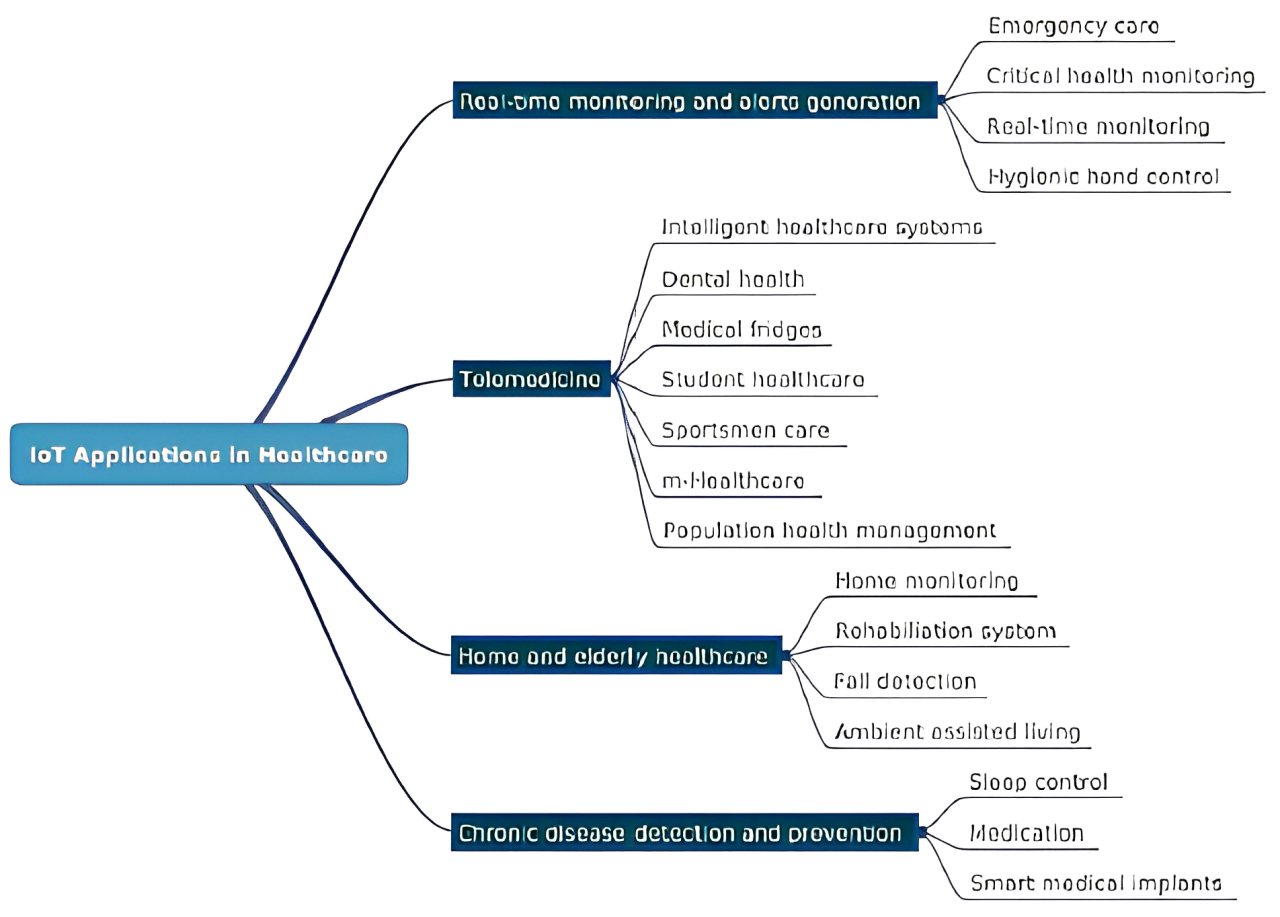
\includegraphics[width=0.75\textwidth]{img/bp/iot-healthcare (1).png}
    \caption{Indeling van IoT-toepassingen in de gezondheidszorg}
    \label{fig:Figuur10}
    \textit{Source: \autocite{Naresh2020}}
\end{figure}

Volgens een recente studie uitgevoerd door \autocite{Singh2023} is het perfect mogelijk om IoT te implementeren in de gezondheidszorg. Echter concludeert het onderzoek dat IoT een gunstige invloed heeft en dit ondanks de beperkingen in “energie, processing en opslag”. Verder benadrukt de studie dat IoT een “veelbelovende technologie” is bij het besparen van tijd en moeite voor het medische personeel. 

\subsection{Huidige implementaties van IoT in de gezondheidszorg}
Een overzicht van implementaties van IoT in het gezondheidszorg: zie figuur \ref{tab:IoT_healthcare}

\begin{table}[h]
    \centering
    \tiny
    \caption{IoT-implementaties in gezondheidszorgstudies \autocite{Mieronkoski2017, Uddin2019, ElZouka2021, Patan2020}}
    \begin{tabularx}{\textwidth}{|p{2cm}|p{1.5cm}|p{3.5cm}|p{3.5cm}|X|}
        \hline
        \textbf{Author and Year} & \textbf{Country} & \textbf{Objectives} & \textbf{IoT Applications} & \textbf{Conclusion} \\
        \hline
        Riitta Mieronkoski  
        & Finland  
        & Voorstellen van IoT aan verpleegkundigen door de stand van zaken over IoT te onderzoeken die betrekking heeft op verpleegkundige zorg in ziekenhuizen.          
        & IoT-innovaties zijn geïdentificeerd in vier verpleegactiviteiten: "comprehensive assessment, periodical clinical reassessment, activities of daily living en care management".  
        & IoT biedt innovaties in verpleegkundige zorg, maar deze innovaties bevinden zich nog in de beginfase. \\  
        \hline
        Md. Zia Uddin  
        & Norway  
        & Ontwikkelen van een systeem dat menselijke activiteiten kan voorspellen door gebruik te maken van wearable healthcare sensors en een Recurrent Neural Network (RNN) op een edge-device.  
        & Verschillende wearable sensoren (ECG, magnetometer, accelerometer en gyroscoop) worden gebruikt voor het monitoren van menselijke activiteiten.  
        & Het gebruik van RNN samen met wearable sensoren op een edge-apparaat vormt een effectief systeem voor het voorspellen van menselijke activiteiten. \\  
        \hline
        Hesham A. El Zouka, Mustafa M. Hosni  
        & Egypt  
        & Het doel is om een slim healthcare-model te ontwikkelen dat automatisch de prioriteit van patiënten bepaalt op basis van gegevens uit sensoren.  
        & IoT-apparaten, WMSN en RFID monitoren patiëntgegevens zoals temperatuur, hartslag en bloeddruk.  
        & Het integreren van fuzzy, AI en IoT biedt real-time monitoring en veilige communicatie. Dit systeem zorgt voor betere patiëntenzorg. \\  
        \hline
        Rizwan Patan, G S Pradeep Ghantasala, Ramesh Sekaran, Deepak Gupta, Manikandan Ramachandran  
        & India  
        & GFB-CNN vermindert communicatie-overhead en responstijd en verhoogt de nauwkeurigheid van medische data-analyse.  
        & IoT wordt toegepast in smart healthcare. IoT-sensoren verzamelen en verzenden medische data voor real-time analyse.  
        & De GFB-CNN-methode verbetert de analyse van medische data door de analysetijd te verkorten. \\  
        \hline
    \end{tabularx}
    \label{tab:IoT_healthcare}
\end{table}


%\section{Voordelen en uitdagingen van IoT in de gezondheidszorg}
%In dit deel worden de voor- en nadelen van IoT in de gezondheidszorg opgenomen volgens de literatuur. Hierbij wordt er rekening gehouden met hoe IoT de gezondheidszorg beïnvloedt en hoe deze de gezondheidszorg heeft getransformeerd. In de volgende secties worden eerst de voordelen besproken gevolgd door de uitdagingen die hierbij horen.


%\subsection{Voordelen}
%Door zorgverleners in staat te stellen om IoT te benutten is het mogelijk om “patiëntresultaten te verbeteren, het gebruik van middelen te optimaliseren, de operationele efficiëntie te verhogen, en patiënten in staat stellen actief deel te nemen aan hun eigen zorg wordt mogelijk gemaakt” \autocite{Inzole2024}. Er zijn een onbeperkt aantal mogelijkheden om de gezondheidszorg te verbeteren door gebruik te maken van IoT, hier zijn enkele belangrijke verbeteringen die IoT brengt \autocite{Inzole2024, Abdulmalek2022}. 

%\begin{itemize}
%    \item Beter behandeling van patiënten
%    \item Vroeg opsporen van ziektes
%    \item Kost van behandeling verminderen
%    \item Beter monitoren en beheren van patiënten
%    \item Verhoogd efficiëntie en verbeterde middelen gebruik
%\end{itemize}

%Ondanks de vele voordelen introduceert IoT ook een aantal uitdagingen, deze worden in het volgende sectie besproken. 

%\subsection{Uitdagingen}
%Hoewel IoT belangrijke voordelen levert aan de gezondheidszorg, brengt IoT nog steeds veel problemen met zich mee zoals aangetoond door figuur \ref{fig:Figuur13}. Het analyseren van deze problemen is essentieel voordat IoT geïmplementeerd kan worden om mitigerende strategieën te bedenken zodat IoT op een verantwoordelijke manier kan uitgerold worden. Hier zijn enkele nadelen van IoT in het gezondheidszorgomgeving \autocite{Inzole2024, Abdulmalek2022}.


%\begin{itemize}
%    \item Security
%    \item Privacy
%    \item Interoperabiliteit
%    \item Naleving van regelgeving
%    \item Ethische consideraties
%\end{itemize}

%\begin{figure}[h]
%    \centering
%    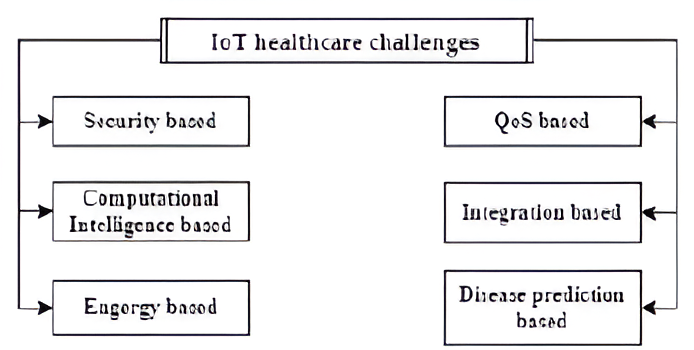
\includegraphics[width=0.60\textwidth]{img/bp/iot-challenges.png}
%    \caption{Nadelen van IoT in het gezondheidszorg}
%    \label{fig:Figuur13}
%    \textit{Source: \autocite{Abdulmalek2022}}
%\end{figure}


%In het volgende deel worden de uitdagingen verder toegelicht, met een specifiek focus op de beveiligings- en ethische kwesties.


%\section{Beveiliging en ethische kwesties van IoT in de gezondheidszorg}
%Met het naadloze integratie van IoT in ziekenhuizen worden patiënten gegevens zorgvuldig verzameld en geanalyseerd waardoor iedere patiënt dezelfde medische diensten kan verwachten. Het gebruik van IoT zorgt ervoor dat patiënten zich niet meer constant hoeven te verplaatsen tussen het ziekenhuis en woonplaats waardoor het niet alleen de sociale lasten maar ook het financiële druk verlaagd \autocite{Chang2019}. Echter, produceren en verzamelen medische instellingen enorme hoeveelheid data (big data) zoals medische dossiers, ziekenhuisdossiers, medische- en biomedische onderzoeksdossiers \autocite{Mirza2022}. Hierbij ontstaan er verschillende beveiligings- en privacy risico's voor patiëntgegevens en vertrouwelijkheid. Deze hebben ernstige gevolgen voor patiënten maar ook voor het vertrouwen in biomedische onderzoeken \autocite{Pandey2018, Juengst2014}. In de volgende sectie worden de beveiligings- en ethische uitdagingen verder in detail uitgewerkt.

%\subsection{Beveiliging} 
%Security problemen zijn een reden voor bezorgdheden vooral door het “enorme snelheid en volumes” waarin medische data wordt gegenereerd. Security wordt gedefinieerd als de “confidentiality, integrity en availability” van het verzamelde data die door het systeem worden verstuurd \autocite{Mittelstadt2017}. Hierbij ontstaan er verschillende security risico's en dit zoals Spoofing, Injection of false signals, Replay attacks, Eavesdropping \autocite{Mirza2022}. Deze risico's ontstaan door “inadequate privacy policies, menselijke fouten, verouderde of onveilige medische apparaten en technologische incompatibiliteit waardoor patiëntengegevens kwetsbaar worden voor misbruik \autocite{Popescul2018}. Ernstige gevolgen kunnen hieruit volgen, waaronder het verlies van mensenlevens, hierdoor wordt security beschouwt als van primordiaal belang \autocite{Ali2024}. Ondanks de uitdagingen dat security met zich meebrengt in IoT is dit niet de enige uitdaging, in het volgende sectie worden de ethische uitdagingen verder besproken.

%\subsubsection{Ethiek}
%Sociale gedrag normen in IoT omvatten beide ethiek en moraal. Ethiek wordt gedefinieerd als hetgeen dat moreel goed of slecht is, en wat fout of juist is, terwijl moraal gedefinieerd wordt als een standaard van normen en regels voor goed gedrag in de samenleving. Ethische gedrag vereist dat men zich houdt aan de volgende richtlijnen \autocite{AboBakr2017, Xhemajli2021}:

%\begin{itemize}
%    \item Privacy van gegevens
%    \item Toegang tot gegevens
%    \item Integriteit van gegevens
%\end{itemize}

%Ethische problemen volgens \autocite{Zakerabasali2022} zijn een van de meest belangrijke en complexe probleem binnen IoT, waardoor het mitigeren hiervan van hoge prioriteit is tijdens de implementatiefase. Figuur \ref{fig:Figuur14} toont de belangrijkste ethische problemen in IoT. 


%\begin{figure}[h]
%    \centering
%    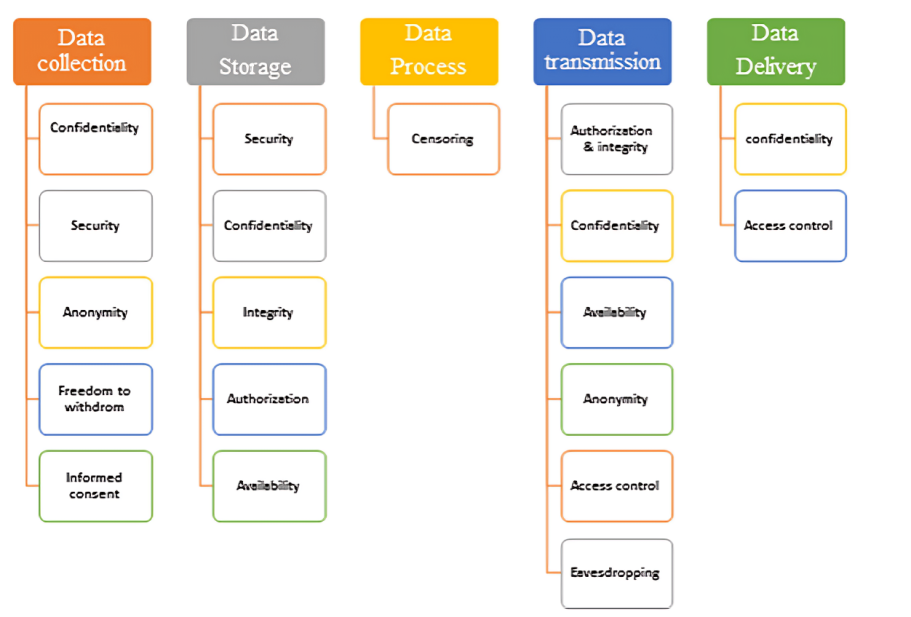
\includegraphics[width=1\textwidth]{img/bp/iot-ethical-issues (1).png}
%    \caption{Ethische kwesties gebaseerd op implementatiefasen van een IoT-systeem.}
%   \label{fig:Figuur14}
%    \textit{Source: \autocite{Zakerabasali2022}}
%\end{figure}

%In het volgende sectie wordt er bekeken naar belangrijke mitigatie strategieën tegen beveiliging en ethische risico's.

%\subsubsection{Mitigatie strategieën}
%De security risico's in IoT kunnen op verschillende manieren gemitigeerd worden zoals het implementeren van “technische maatregelen, policy frameworks en gebruikers educatie”. Deze omvatten de volgende strategieën \autocite{Iwuanyanwu2023}: 

%\begin{itemize}
%    \item Technische maatregelen:“Encryption and Secure Communication, Robust Authentication Mechanism, Software and Firmware Updates en Intrusion Detection Systems (IDS)”
%    \item policy frameworks: “Compliance with Industry Standards and Regulations, Legal Frameworks for IoT Security“
%    \item gebruikers educatie: “Training Programs for End-Users, Promoting Secure IoT Practices”
%\end{itemize}

%De ethische risico's kunnen op diverse manieren worden aangepakt, maar het idee is dat één enkele mitigatie strategie niet genoeg kan zijn om meerdere ethische problemen te behandelen. Daarom wordt er voorgesteld om verschillende strategieën te combineren zoals: 

%\begin{itemize}
%    \item “ethisch gedrag bij het programmeren”
%    \item “whitebox-algoritmen”
%    \item “blackbox-validatie”
%    \item “algoritmische sociale contracten”
%    \item “omhullende IoT-systemen”
%    \item “richtlijnen en ethische code voor IoT-ontwikkelaars”
%%\end{itemize}

%Het combineren van deze strategieën kan ervoor zorgen dat alle aspecten van verschillende ethische risico's behandeld worden \autocite{Loke2019}. Na het bespreken van de beveiliging en ethische kwesties van IoT wordt de focus gelegd op de kern van het onderzoek. In de volgende secties zullen verschillende onderdelen besproken worden die hiermee verband houden. Eerst zullen de wachttijden op de A\&E-afdelingen behandeld worden. Vervolgens zal de impact hiervan op het zorgkwaliteit uitgebreid worden besproken. Tot slot worden de IoT-devices die deze probleem kunnen verhelpen opgesomd en besproken. 

\section{Wachttijden in A\&E-afdelingen}
De vraag naar spoedeisende hulp is in veel landen gestegen zoals in Engeland,
Australië, Stockholm, Schotland en Noord-Ierland waardoor het steeds moeilijker is om doorlooptijden kort te houden. Verschillende factoren zijn de oorzaak van dit probleem zoals het veroudering van de populatie, complexere ziektes en de toenemende vraag van patiënten voor spoedeisende zorg. Volgens studies uitgevoerd door \autocite{Paling2020, Friebel2020} door is bedbezetting nauw verbonden met hoge wachttijden, zoals aangetoond in Figuur \ref{fig:Figuur11} is er een correlatie tussen de hoge wachttijden en bedbezetting.

\begin{figure}[h]
    \centering
    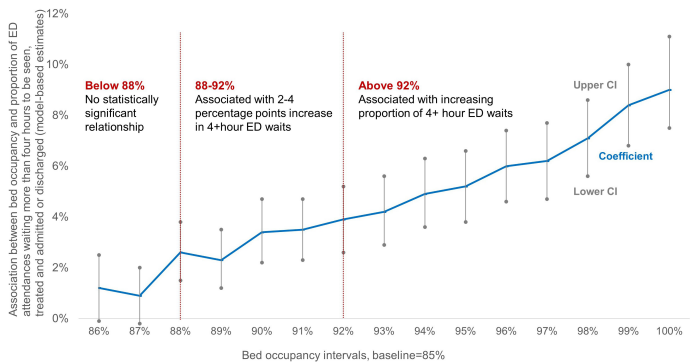
\includegraphics[width=0.80\textwidth]{img/bp/bed-occupancy.png}
    \caption{Plot dat een niet-lineaire relatie toont tussen bedbezettingen intervallen en proportie van patiënten die meer dan vier uur spenderen in de A\&E-afdeling}
    \label{fig:Figuur11}
    \textit{Source: \autocite{Paling2020}}
\end{figure}

Om dit probleem tegen te gaan hebben meerdere landen een wachttijdsstandaard geïmplementeerd om de wachttijden in kaart te brengen en deze gevolgen te verminderen \autocite{Paling2020}. In de Verenigd Koninkrijk bijvoorbeeld is “tijdigheid” een cruciaal aspect in het kwaliteit van spoedeisende hulp, en de wachttijddoelstellingen van de National Health Service zijn hierop gebaseerd voor A\&E afdelingen in het hele Verenigd Koninkrijk. Deze wachttijddoelstellingen eisen dat 98 percent van de A\&E patiënten binnen de vier uur van de aankomst worden ontslagen, overgeplaatst of opgenomen worden in een ziekenhuis \autocite{Mayhew2008, Izady2012}. 


Echter wordt er aan deze vier-uur standaard nauwelijks voldaan. Volgens een studie uitgevoerd door \autocite{Baker2024} is het percentage van patiënten die langer dan vier uur in de A\&E-afdelingen spenderen tussen 2015 en 2020 sterk toegenomen. Verder toont het onderzoek dat er een nieuw record bereikt is met 50,4\% van patiënten die langer dan vier uur wachten op behandeling in A\&E-afdelingen zoals aangetoond door figuur \ref{fig:Figuur12}. Dit vormt een duidelijke overtreding van de vier-uur norm van de NHS. Deze richtlijn houdt in dat tenminste 95\% van de patiënten binnen vier uur moeten worden opgenomen, overgebracht en ontslagen. \autocite{NationalStatisticsONS2024}.

\begin{figure}[h]
    \centering
    \includegraphics[width=0.80\textwidth]{img/bp/patiënts_over_4_hours.png}
    \caption{Percentage van patiënten die langer dan 4 uur wachten}
    \label{fig:Figuur12}
    \textit{Source: \autocite{Baker2024}}
\end{figure}

% Link volgende stuk
Deze lange wachttijden hebben serieuze gevolgen op de patiëntentevredenheid en zorgkwaliteit zoals besproken in het volgende hoofdstuk.

\subsection{Impact van wachttijden op de zorgkwaliteit}
Volgens verschillende studies hebben langdurige wachttijden negatieve gevolgen voor zowel patiënten als de zorgkwaliteit. Studies uitgevoerd door \autocite{Vainieri2020, QuintonJ.Nottingham2018, Bleustein2014} benadrukken de negatieve impact van de wachttijden op de patiëntentevredenheid. Deze onderzoeken tonen aan dat lange wachttijden een ongunstige invloed op de tevredenheid van patiënten, vooral in het vertrouwen van de zorgverleners en kwaliteit van de zorg. Verder benadrukt een studie uitgevoerd door \autocite{Paling2020} nog ernstigere gevolgen voor patiënten, deze onderzoek heeft een verband gesteld tussen wachttijden in A\&E-afdelingen en een hogere mortaliteit en verergeren van resultaten voor patiënten. Echter, zijn patiënten niet de enige die door de lange wachttijden worden beïnvloed, volgens \autocite{Osborne2015} ervaren duizenden verpleegsters in Engeland moeilijkheden bij het omgaan met de lange A\&E-wachttijden, het artikel vermeldt verder een quote door de toenmalige RCN emergency care association chair, Janet Youd, die aangaf dat 'verpleegsters zijn uitgeput en velen worden ziek door stressgerelateerde aandoeningen'. Onderzoekers hebben onlangs de werkomstandigheden van NHS werknemers onderzocht. De studie toont dat 40\% van alle ziekten bij het personeel te wijten is aan stress. Verder wijst het onderzoek uit dat de “overheersende stressfactor” wordt veroorzaakt door de hoge werkdruk \autocite{Ravalier2020}. \autocite{Vainieri2020} onderlijnt overbevolking als oorzaak van de hoge werkbelasting, en dit in A\&E departementen in diverse westerse landen. Hierbij wordt er verder benadrukt van de ernst van het probleem voor zowel patiënten als zorgverleners. Deze probleem kan door diverse IoT devices verholpen worden. Dit wordt in het volgende sectie verder besproken. 


% \autocite{Vainieri2020} onderlijnt overbevolking als oorzaak van de hoge werkbelasting, en dit in A\&E departementen in diverse westerse landen. Om beter te begrijpen hoe IoT dit probleem kan oplossen, is het noodzakelijk om dieper in te gaan op wat IoT precies inhoudt. Over het algemeen verwijst Internet of things (IoT) naar een model dat verschillende technologieën omvat. Anders gezegd, is het een netwerk van elektronische apparaten die met elkaar of met de cloud communiceren via het internet. De afgelopen twee decennia hebben een grote invloed gehad op de snelle vooruitgang van IoT \autocite{Almutairi2024}, hierdoor is het aantal aangesloten IoT devices sterk gestegen, met 7.74 miljard in 2019, 10.7 miljard in 2021 \autocite{Dawod2022} en 25.44 miljard tegen 2030 \autocite{Dawod2022}. Sensoren, camera's en gelijkaardige apparaten worden al “geïntegreerd” in “woningen” en “voertuigen” \autocite{Dawod2022} en geïmplementeerd over verschillende sectoren zoals de “gezondheidszorg, landbouw, productie” en slimme steden \autocite{Almutairi2024}.

\section{Internet of Things bij het verkorten van wachttijden in het gezondheidszorg}
IoT heeft zich veelbelovend getoond bij het verminderen van wachttijden in de gezondheidszorg en het verbeteren van de patiëntenzorg \autocite{Bhatt2017}. Diverse studies tonen verschillende implementaties van IoT in de gezondheidszorg en in wachtruimtes \ref{wachtruimte} met als doel om wachttijden te verminderen, zoals aangetoond in tabel \ref{tab:IoT_waiting_time_reduction_healthcare} 

\begin{table}[h]
    \centering
    \tiny
    \caption{Studies: IoT implementaties om wachttijden te verminderen in gezondheidszorg \autocite{Sierra2017, McNabb2018, Alabduljabbar2022, Bhatt2017, Fischer2020, Chandy2019}}
    \begin{tabularx}{\textwidth}{|p{1.7cm}|p{0.9cm}|p{3.5cm}|p{3.5cm}|X|}
        \hline
        \textbf{Author and Year} & \textbf{Country} & \textbf{Objectives} & \textbf{IoT Applications} & \textbf{Conclusion} \\
        \hline
        Pedro Santiago Sierra, Jeyson Bolivar Siculaba, Giovanny Mauricio Tarazona   
        & Colombia 
        & Ontwikkelen van een mobile applicatie waarmee gebruikers instaat zijn om de verschillende wachttijden van diverse zorgpunten te raadplegen. 
        & IoT-gebaseerde sensoren worden op de zorgpunten geïmplementeerd om real-time data te verzamelen 
        & De ontwikkeling en simulatie tonen aan dat de applicatie de gebruiker in staat stelt om zorgpunten te selecteren met de kortste wachttijden. \\
        \hline
        Tim McNabb, Trina Myers*, Kristin Wicking, Lei Lei en Wei Xiang 
        & Australia 
        & Optimaliseren van high-value clinical spaces in de gezondheidszorg door gebruik te maken van IoT. 
        & Drie types werden gebruikt in de eindfase: “infra-red break-beam”, “photovoltaic infra-red (PIR)” en  “photovoltaic array” 
        & De conclusie toont aan dat PIR-sensoren niet voldoende zijn om bezettingen te detecteren.  \\
        \hline
        Reham Alabduljabbar* 
        & Saudi Arabia 
        & Het doel is om een location-aware mobile-based solution (UrNext) te introduceren en te evalueren om wachttijden te verminderen. 
        & Bluetooth Low-Energy (BLE) technology wordt gebruikt om locatie te bieden in ziekenhuizen 
        & UrNext biedt de mogelijkheid om wachttijden te verminderen door gebruik te maken van BLE-technologieën. \\
        \hline
        Yesha Bhatt, Chintan Bhatt 
        & India 
        & Wachttijden elimineren en ziekenhuis bezoeken verminderen door het implementeren van remote healthcare via IoT.
        & Deze implementatie maakt gebruik van Medical devices met IoT features, Biomedical sensors, Smart devices voor patient-nurse connectivity, 24/7 patient monitoring systems.
        & IoT in de gezondheidszorg is steeds in de ontwikkeling phase, verschillende uitdagingen moeten nog geadresseerd worden maar het heeft de potentieel om de industrie te revolutioneren.   \\
        \hline
        Abraham Chandy
        & India 
        & Wachttijden verminderen en medische beeldvorming verbeteren door automatisatie en optimalisatie.
        & IoT wordt gebruikt in medische beeldvorming en medische apparatuur.
        & IoT-enabled medische beeldvorming kan de efficiëntie van de gezondheidszorg verbeteren, kosten verminderen en diagnoses verbeteren.    \\
        \hline
        Gabriel Souto Fischer,
        Rodrigo da Rosa Righ,
        Gabriel de Oliveira Ramos,
        Cristiano André da Costa,
        Joel J.P.C. Rodrigues
        & Brazil 
        & ElHealth heeft als doel om de toewijzing van de gezondheidszorgprofessional te optimaliseren door gebruik te maken van IoT om wachttijden te verminderen.
        & Occupancy sensors, patiënt monitoring systemen en omgeving sensoren worden gebruikt om ruimte gebruik en behoeften van patiënten bij te houden.
        & De ElHealth maakt gebruik van voorspellingen en dynamische personeel toewijzing om wachttijden te verminderen processen te optimaliseren.    \\
        \hline
    \end{tabularx}
    \label{tab:IoT_waiting_time_reduction_healthcare}
\end{table}

\subsection{Implementaties van IoT in wachtruimtes} \label{wachtruimte}

\begin{table}[h]
    \centering
    \tiny
    \caption{Studies: IoT implementaties om wachttijden te verminderen in gezondheidszorg \autocite{Spoladore2024, Ghazal2015}}
    \begin{tabularx}{\textwidth}{|p{2.5cm}|p{1cm}|p{4cm}|p{4.5cm}|p{3cm}|}
        \hline
        \textbf{Author and Year} & \textbf{Country} & \textbf{Objectives} & \textbf{IoT Applications} & \textbf{Conclusion} \\
        \hline
        Daniele Spoladore, Marta Mondellini, Atieh Mahroo, Irene Alice Margherita Chicchi Giglioli, Stefano De Gaspari, Daniele Di Lernia, Giuseppe Riva, Elena Bellini, Nicoletta Setola, Marco Sacco   
        & Italy 
        & Onderzoeken hoe IoT, AI en Virtual reality een wachtruimte kan transformeren in een smart omgeving. 
        & De Age-IT prototype maakt gebruik van IoT sensoren, AI en virtual reality.
        & Dit systeem biedt een significante stap bij het transformeren van traditionele wachtruimtes in een smart omgeving en het omzetten van wachttijden in diagnostische en therapeutische activiteiten. \\
        \hline
        M. Ghazal, Rania Hamouda, Samr Ali
        & Bahrain 
        & Het doel is om de queue management te verbeteren door de service kwaliteit te verhogen en wachttijden te verminderen
        & Het systeem maakt gebruik van ESP32 om live queue data te versturen.
        & Het systeem werkt zoals weergegeven in de studie.  \\
        \hline
    \end{tabularx}
    \label{tab:IoT_waiting_time_reduction_waitingroom}
\end{table}


\section{Plaatsing strategieën van IoT}
De plaatsing van een IoT device wordt gecategoriseerd worden in twee diverse plaatsing strategieën, de fysieke plaatsing en netwerk plaatsen. In de netwerkplaatsing wordt de focus gelegd op de plaatsing van de IoT-gateways. Aangezien deze buiten de scope van het onderzoek vallen, zijn alleen de fysieke plaatsing en relevante aspecten van belang. Deze worden in de volgende sectie verder toegelicht.

\subsection{Physical placement}
Fysieke plaatsing is de manier waarop een device “strategisch geplaatst” wordt voor een betere netwerk performantie en dekking \autocite{Xia2018}. Zie tabel \ref{tab:placement_strategies} voor een overzicht van diverse fysieke plaatsing strategieën.

\begin{table}[h]
    \centering
    \tiny
    \caption{Physical Placement Strategies for IoT Devices, \autocite{Tinglib2012, Alablani2019, Badiger2022, Chen2023, Krishnachalitha2020, Patil2021, Paul2020}}
    \begin{tabular}{|l|p{4cm}|p{5cm}|p{4cm}|} % Adjusted last column width
        \hline
        \textbf{Strategy} & \textbf{Goal} & \textbf{Approach/Method} & \textbf{Benefits} \\ \hline
        Uniform Random Deployment & Devices worden random verspreid om dekking te hebben over een gebied. Uniform deployment is een gemeenschappelijke strategie voor het uitrollen van IoT devices en sensoren in een wireless netwerk  & Devices worden op een uniforme wijze verspreid over een bepaald gebied. & Makkelijk te implementeren, maar heeft weinig dekking en is minder veerkrachtig tegen aanvallen. \\ \hline
        Grid-Based Deployment & biedt predictive en gestructureerde dekking voor wireless netwerken  & Devices worden uitgerold in een geometrische pattern zoals square grids, triangular grids, or hexagonal grids om voor een uniforme dekking te zorgen. De square grid heeft een hogere performantie in de dekking van gebieden terwijl de andere beter in end-to-end delay zijn. & voorspelbaar en makkelijk te analyseren dekking gebied. \\ \hline
        Cluster-Based Deployment & Heeft als doel om data aggregation te optimaliseren en het verminderen van energie consumptie. & Devices worden gegroepeerd in clusters, een centrale nood worden vervolgens gebruikt voor data aggregation en energy efficiënte solutions. & Verminderd data redundancy en communicatie overhead. \\ \hline
        Mobility-Aware Deployment & De IoT devices worden geplaatst op basis van de beweging pattern van devices of users & Devices worden dynamisch geplaatst volgens voorspelde beweging patterns. & Verminderd de energie consumptie en verbetert de plaatsing efficiëntie \\ \hline
        Fixed Placement & Zorgt ervoor dat de data verzameling consistent en betrouwbaar is. & Devices worden op permanente locaties geïnstalleerd, dit zorgt voor een sterke netwerk performantie en verbruik van middelen. & Betrouwbaar en makkelijk te onderhouden \\ \hline
    \end{tabular}
    \label{tab:placement_strategies}
\end{table}


%\subsection{Network placement}
%In Netwerk plaatsing wordt de focus gelegd op de plaatsing van de IoT gateways, om kosten te verminderen en performantie te verhogen \autocite{Patil2021, Patil2021a}. Zie tabel \ref{tab:network_placement_strategies} voor enkele praktische voor beelden van Netwerk strategieën.

%\begin{table}[h]
%    \tiny
%    \caption{Network Placement Strategies for IoT Gateways, \autocite{Mnguni2019, Patil2021a, Patil2021, Beuchat2019, Kotagi2017, Nezami2020, Matni2020, Dautov2017}}
%    \begin{tabular}{|p{3.5cm}|p{6.5cm}|p{4.5cm}|}
%        \hline
%        \textbf{Strategy} & \textbf{Description} & \textbf{Benefits} \\ \hline
%        Fixed Gateway Placement & Gateways worden strategisch geplaatst om de dekking te maximaliseren en de netwerk performantie te verbeteren. & Betrouwbare kwaliteit van de service en vermindering van de kosten. \\ \hline
%        Distance-Based Optimization & Gateways worden geplaatst door middel van optimalisatietechnieken zoals Euclidische of Manhattan-afstand om energieverbruik en latentie te minimaliseren. & Efficiënter gebruik van netwerkbronnen en minder energieverbruik. \\ \hline
%        Load-Balanced Placement & Gateways worden geplaatst op basis van de verkeersbelasting. Load balancing is essentieel bij het verbeteren van netwerk performantie en vermijden van congesties. & Consequente verbetering in netwerk performantie en vertraging. \\ \hline
%        Dynamic Gateway Placement & Gateways wijzigen hun positie op basis van veranderende netwerkcondities, zoals gebruikersmobiliteit of variërende dataverkeerpatronen. & Verminderen van de kosten en betere QoS in dynamische IoT-omgevingen. \\ \hline
%        Hierarchical Gateway Deployment & Meerdere niveaus van gateways worden gebruikt om de belasting te verminderen en reactietijd te verhogen. De lagere niveaus verwerken lokaal, terwijl de hogere niveaus verantwoordelijk zijn voor het versturen van data naar de cloud. & Efficiëntere data-agregatie en verminderde latentie. \\ \hline
%    \end{tabular}
%    \label{tab:network_placement_strategies}
%\end{table}


%\section{Evaluatie van software voor IoT-implementaties}
%Diverse software worden gebruikt om communicatie, verwerking, analyse mogelijk te maken in IoT-implementaties. Het doel van deze sectie is om verschillende software te identificeren door diverse studies te verkennen. Het volgende tabel \ref{tab:software_literatuurstudie} toont een overzicht van onderzoeken

%\begin{table}[h]
%    \tiny
%    \caption{Overzicht van onderzoeken naar softwaregebruik in IoT-implementaties, \autocite{Vikash2020}, \autocite{Giacobbe2020}}
%    \begin{tabular}{|p{2.5cm}|p{4.7cm}|p{5.7cm}|p{3.5cm}|}
%        \hline
%        \textbf{Author} & \textbf{Software} & \textbf{Application} & \textbf{Key findings} \\ 
%        \hline
%        Vikash, Lalita Mishra, Shirshu Varma & Apache NiFi & Automatiseert datastroom tussen systemen  & NiFi biedt hoog throughput en lage latency, is ideal voor gebruik met IoT \\ 
%        \hline
%        Vikash, Lalita Mishra, Shirshu Varma & Apache Storm & Verwerken van real-time, unbounded datastreams & Neemt de kortste opstarttijd. \\ 
%        \hline
%        Vikash, Lalita Mishra, Shirshu Varma & Apache Apex & Ondersteunt streams en batch processing voor real-time big data applications & Minst bruikbare solution voor IoT, biedt low throughput, hoog response time, en maximum jitter. \\ 
%        \hline
%        Vikash, Lalita Mishra, Shirshu Varma & Spark Streaming & Verwerkt in real-time batch data door de taken te verdelen over clusters & N.V.T. \\ 
%        \hline
%        Vikash, Lalita Mishra, Shirshu Varma & Apache Flink & Real-time verwerking van batch data door master, slave architectuur te gebruiken voor parallel uitvoer van taken& Minst scalable solution.  \\ 
%        \hline
%        Maurizio Giacobbe, Chakib Chaouch, Marco Scarpa, Antonio Puliafito & InfluxDB & Time series data store voor IoT en real-time analyse & Verzamelt tijdstempels, id's en sensorgegevens zoals temperatuur, helderheid, kooldioxide in smart city-platform. \\ 
%        \hline
%        Robert Stackowiak & Microsoft Azure IoT Suite: Azure IoT Hub & Maakt verbinding en beheer van IoT-devices mogelijk. & N.V.T. \\ 
%        \hline
%        Robert Stackowiak & Microsoft Azure IoT Suite: Azure Digital Twins & Maakt gebruk van ruimtelijke intelligentiegrafieken om een virtuele weergave van de fysieke wereld te maken & N.V.T. \\ 
%        \hline
%        Robert Stackowiak & Microsoft Azure IoT Suite: Azure Stream Analytics & Verwerkt hoge volumes streaming data van devices via SQL queries  & N.V.T. \\ 
%        \hline
%        Robert Stackowiak & Microsoft Azure IoT Suite: Azure Time Series Insights & Maakt de analyse en visualisatie van time series data van IoT-devices.   & N.V.T. \\ 
%        \hline
%        Robert Stackowiak & Microsoft Azure IoT Suite: Azure Databricks & Biedt real-time data verwerking, machine learning en autoscalling van IoT  & N.V.T. \\ 
%        \hline
%        Robert Stackowiak & Microsoft Azure IoT Suite: Azure Data Lake Storage & Azure Data Lake Storage Gen2 combineert de kosteneffectiviteit van Azure Blob Storage met verbeterde functies voor het bestandssysteem  & N.V.T. \\ 
%        \hline
%        Robert Stackowiak & Microsoft Azure IoT Suite: Azure HDInsight & Verwerkt en analyseert big data en ondersteunt diverse open-source frameworks& N.V.T. \\ 
%        \hline
%    \end{tabular}
%       \label{tab:software_literatuurstudie}
%\end{table}



%\subsection{Vergelijking: Traditionele versus IoT-gebaseerde wachttijdsreductie}

% De term 'Internet of Things' is ontstaan in 1999, toen Kevin Ashton, een Britse technologiepionier, verschillende objecten probeerde te verbinden met het internet door gebruik te maken van RFID-tags \autocite{Bassi2013, Rejeb2023}.


%Twintig jaar later wordt IoT ingezet in verschillende sectoren, zoals gezondheidszorg, transport, slimme steden, nutsbedrijven, milieu, veiligheid en nog veel meer. \autocite{Khan2019}


% in het gezondheidszorg wordt IoT gebruikt

%De gezondheidszorg heeft de voorbije jaren een indrukwekkende groei gekend dankzij de vooruitgang in IoT \autocite{Rejeb2023}

% Tip: Begin elk hoofdstuk met een paragraaf inleiding die beschrijft hoe
% dit hoofdstuk past binnen het geheel van de bachelorproef. Geef in het
% bijzonder aan wat de link is met het vorige en volgende hoofdstuk.

% Pas na deze inleidende paragraaf komt de eerste sectiehoofding.

% Dit hoofdstuk bevat je literatuurstudie. De inhoud gaat verder op de inleiding, maar zal het onderwerp van de bachelorproef *diepgaand* uitspitten. De bedoeling is dat de lezer na lezing van dit hoofdstuk helemaal op de hoogte is van de huidige stand van zaken (state-of-the-art) in het onderzoeksdomein. Iemand die niet vertrouwd is met het onderwerp, weet nu voldoende om de rest van het verhaal te kunnen volgen, zonder dat die er nog andere informatie moet over opzoeken \autocite{Pollefliet2011}.

% Je verwijst bij elke bewering die je doet, vakterm die je introduceert, enz.\ naar je bronnen. In \LaTeX{} kan dat met het commando \texttt{$\backslash${textcite\{\}}} of \texttt{$\backslash${autocite\{\}}}. Als argument van het commando geef je de ``sleutel'' van een ``record'' in een bibliografische databank in het Bib\LaTeX{}-formaat (een tekstbestand). Als je expliciet naar de auteur verwijst in de zin (narratieve referentie), gebruik je \texttt{$\backslash${}textcite\{\}}. Soms is de auteursnaam niet expliciet een onderdeel van de zin, dan gebruik je \texttt{$\backslash${}autocite\{\}} (referentie tussen haakjes). Dit gebruik je bv.~bij een citaat, of om in het bijschrift van een overgenomen afbeelding, broncode, tabel, enz. te verwijzen naar de bron. In de volgende paragraaf een voorbeeld van elk.

% \textcite{Knuth1998} schreef een van de standaardwerken over sorteer- en zoekalgoritmen. Experten zijn het erover eens dat cloud computing een interessante opportuniteit vormen, zowel voor gebruikers als voor dienstverleners op vlak van informatietechnologie~\autocite{Creeger2009}.

% Let er ook op: het \texttt{cite}-commando voor de punt, dus binnen de zin. Je verwijst meteen naar een bron in de eerste zin die erop gebaseerd is, dus niet pas op het einde van een paragraaf.

%\begin{figure}
%  \centering
%  \includegraphics[width=0.8\textwidth]{grail.jpg}
%  \caption[Voorbeeld figuur.]{\label{fig:grail}Voorbeeld van invoegen van een figuur. Zorg altijd voor een uitgebreid bijschrift dat de figuur volledig beschrijft zonder in de tekst te moeten gaan zoeken. Vergeet ook je bronvermelding niet!}
%\end{figure}

%\begin{listing}
%  \begin{minted}{python}
%    import pandas as pd
%    import seaborn as sns

%    penguins = sns.load_dataset('penguins')
%    sns.relplot(data=penguins, x="flipper_length_mm", y="bill_length_mm", hue="species")
%  \end{minted}
%  \caption[Voorbeeld codefragment]{Voorbeeld van het invoegen van een codefragment.}
%\end{listing}

%\lipsum[7-20]

%\begin{table}
%  \centering
%  \begin{tabular}{lcr}
%    \toprule
%    \textbf{Kolom 1} & \textbf{Kolom 2} & \textbf{Kolom 3} \\
%    $\alpha$         & $\beta$          & $\gamma$         \\
%    \midrule
%    A                & 10.230           & a                \\
%    B                & 45.678           & b                \\
%    C                & 99.987           & c                \\
%    \bottomrule
%  \end{tabular}
%  \caption[Voorbeeld tabel]{\label{tab:example}Voorbeeld van een tabel.}
%\end{table}


%%=============================================================================
%% Methodologie
%%=============================================================================

\chapter{\IfLanguageName{dutch}{Methodologie}{Methodology}}%
\label{ch:methodologie}

%% TODO: In dit hoofstuk geef je een korte toelichting over hoe je te werk bent
%% gegaan. Verdeel je onderzoek in grote fasen, en licht in elke fase toe wat
%% de doelstelling was, welke deliverables daar uit gekomen zijn, en welke
%% onderzoeksmethoden je daarbij toegepast hebt. Verantwoord waarom je
%% op deze manier te werk gegaan bent.
%% 
%% Voorbeelden van zulke fasen zijn: literatuurstudie, opstellen van een
%% requirements-analyse, opstellen long-list (bij vergelijkende studie),
%% selectie van geschikte tools (bij vergelijkende studie, "short-list"),
%% opzetten testopstelling/\gls{poc}, uitvoeren testen en verzamelen
%% van resultaten, analyse van resultaten, ...
%%
%% !!!!! LET OP !!!!!
%%
%% Het is uitdrukkelijk NIET de bedoeling dat je het grootste deel van de corpus
%% van je bachelorproef in dit hoofstuk verwerkt! Dit hoofdstuk is eerder een
%% kort overzicht van je plan van aanpak.
%%
%% Maak voor elke fase (behalve het literatuuronderzoek) een NIEUW HOOFDSTUK aan
%% en geef het een gepaste titel.

%\section{Oorzakenanalyse}
%Het onderzoek begint met een oorzakenanalyse, deze heeft als doel om het identificeren van de oorzaak/oorzaken van de lange A\&E wachttijden. Bij het uitvoeren van de oorzakenanalyse worden verschillende methodes toegepast om de kern van het probleem te identificeren, zoals een brainstormsessie in combinatie met de 5 Whys-methode \ref{fig:Figuur15}. Zodra diverse oorzaken geïdentificeerd zijn, begint er een analyse door middel van het Fishbone-model \ref{fig:Figuur15} om te voorkomen dat mogelijke onderliggende oorzaken over het hoofd worden gezien. Vervolgens wordt de oorzaak die het meest impact heeft op de wachttijden geïdentificeerd als de hoofdoorzaak. Tot slot zal er bepaald worden of \gls{iot} een oplossing kan zijn tot de hoofdoorzaak.  Verder in het onderzoek wordt er dieper bekeken naar welke \gls{iot} devices gebruikt kunnen worden in de gezondheidszorg, zodra de devices geselecteerd zijn, wordt er op een meer diepgaande wijze onderzocht of \gls{iot} een geschikte oplossing kan bieden.

%\begin{figure}[h]
%    \centering
%    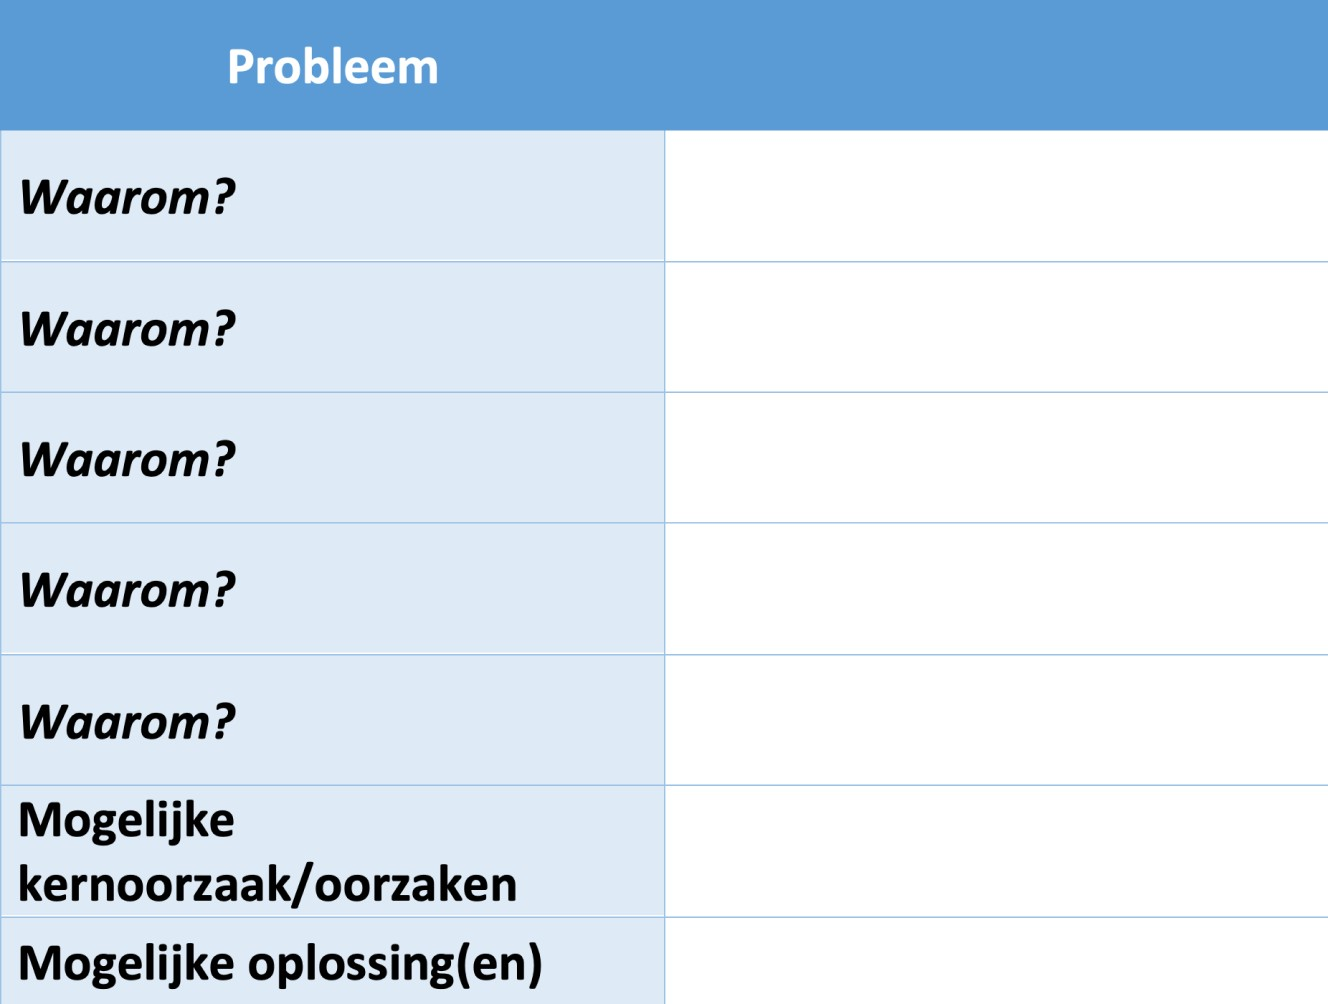
\includegraphics[width=0.5\textwidth]{img/Figuur-5}
%    \caption{5 Whys”-methode}
%    \label{fig:Figuur15}
%    \textit{Source: \autocite{Scharwaechter2023}}
%\end{figure}

%\begin{figure}[h]
%    \centering
%    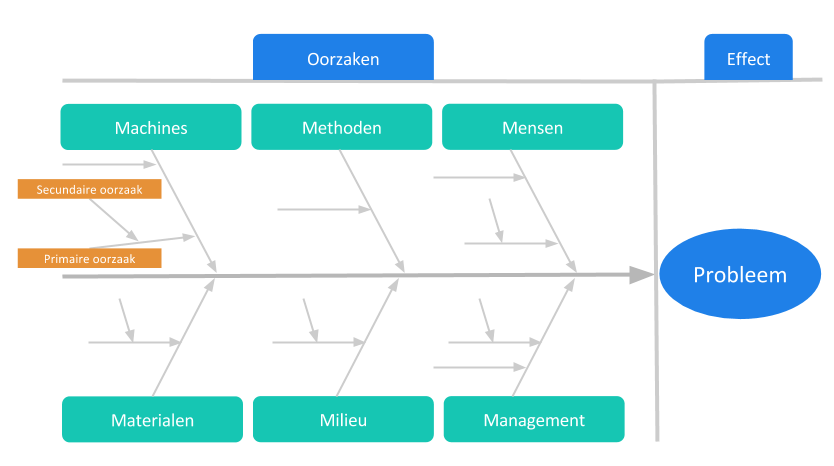
\includegraphics[width=0.7\textwidth]{img/Figuur-6}
%    \caption{De fishbone diagram}
%    \label{fig:Figuur16}
%    \textit{Source: \autocite{Swaen2023}}
%\end{figure}

%Doelstelling

%welke deliverables daar uit gekomen zijn

%welke onderzoeksmethoden je daarbij toegepast hebt

%Verantwoord waarom je op deze manier te werk gegaan bent

%Het onderzoek begint met het uitvoeren van een uitgebreide oorzakenanalyse. Dit is een fundamentele stap bij het identificeren van de oorzaak van de langdurige wachttijden binnen de A\&E afdelingen van ziekenhuizen. De analyse begint met het definiëren van het probleem. Om die reden wordt de “5 Whys”-methode toegepast samen met een brain\-storming-sessie. De “5 Whys”-methode wordt gebruikt om de kern van het probleem te achterhalen door telkens de vraag waar\-om te stellen, \ref{fig:Figuur5} en de oorzaak proberen te identificeren via de brain\-storming-sessie. Zodra diverse oorzaken geïdentificeerd zijn, begint er een analyse door middel van het Fishbone-model. De reden achter het gebruik van dit model is het voorkomen dat mogelijke onderliggende oorzaken over het hoofd worden gezien. Verder biedt het model simpliciteit bij het trekken van conclusies dankzij een visuele representatie tussen de categorisch weergegeven oorzaken en het probleem. Vervolgens is elke oorzaak zorgvuldig bestudeerd, degene die de grootste impact heeft op langdurige wachttijden is geselecteerd als de hoofdoorzaak. Een overweging is vervolgens gemaakt, om te achterhalen of \gls{iot} in het algemeen een oplossing kan zijn voor deze oorzaak. Verder in het onderzoek wordt er dieper bekeken naar welke \gls{iot} devices gebruikt kunnen worden in de gezondheidszorg, zodra de devices geselecteerd zijn, wordt er op een meer diepgaande wijze bekeken hoe de apparaten een oplossing kunnen zijn voor de hoofdoorzaak.

\section{Literatuurstudie van \gls{iot}-oplossingen, sensortypes, analysemethoden en onderzoeksmethoden}
In hoofdstuk \ref{ch:stand-van-zaken} werden verschillende \gls{\gls{iot}}-oplossingen, sensortypes en analysemethoden en onderzoeksmethoden geanalyseerd.

%\section{Geoptimaliseerde servicezones} %

%\begin{table}[h]
%    \centering
%    \tiny
%    \caption{Table with Type, Description, and Image}
%    \begin{tabular}{ | m{3cm} | m{6cm} | m{8cm} | }
%        \hline
%        \textbf{Type} & \textbf{Description} & \textbf{Image} \\ 
%        \hline
%        Type 1: Ziekenhuis/Spoed & Een wachtruimte van een bepaald ziekenhuis afdeling (cardiologie, ophtamologie, enz.. ) of een wachtruimte aan de bali/triage van een spoedafdeling.  & 
%        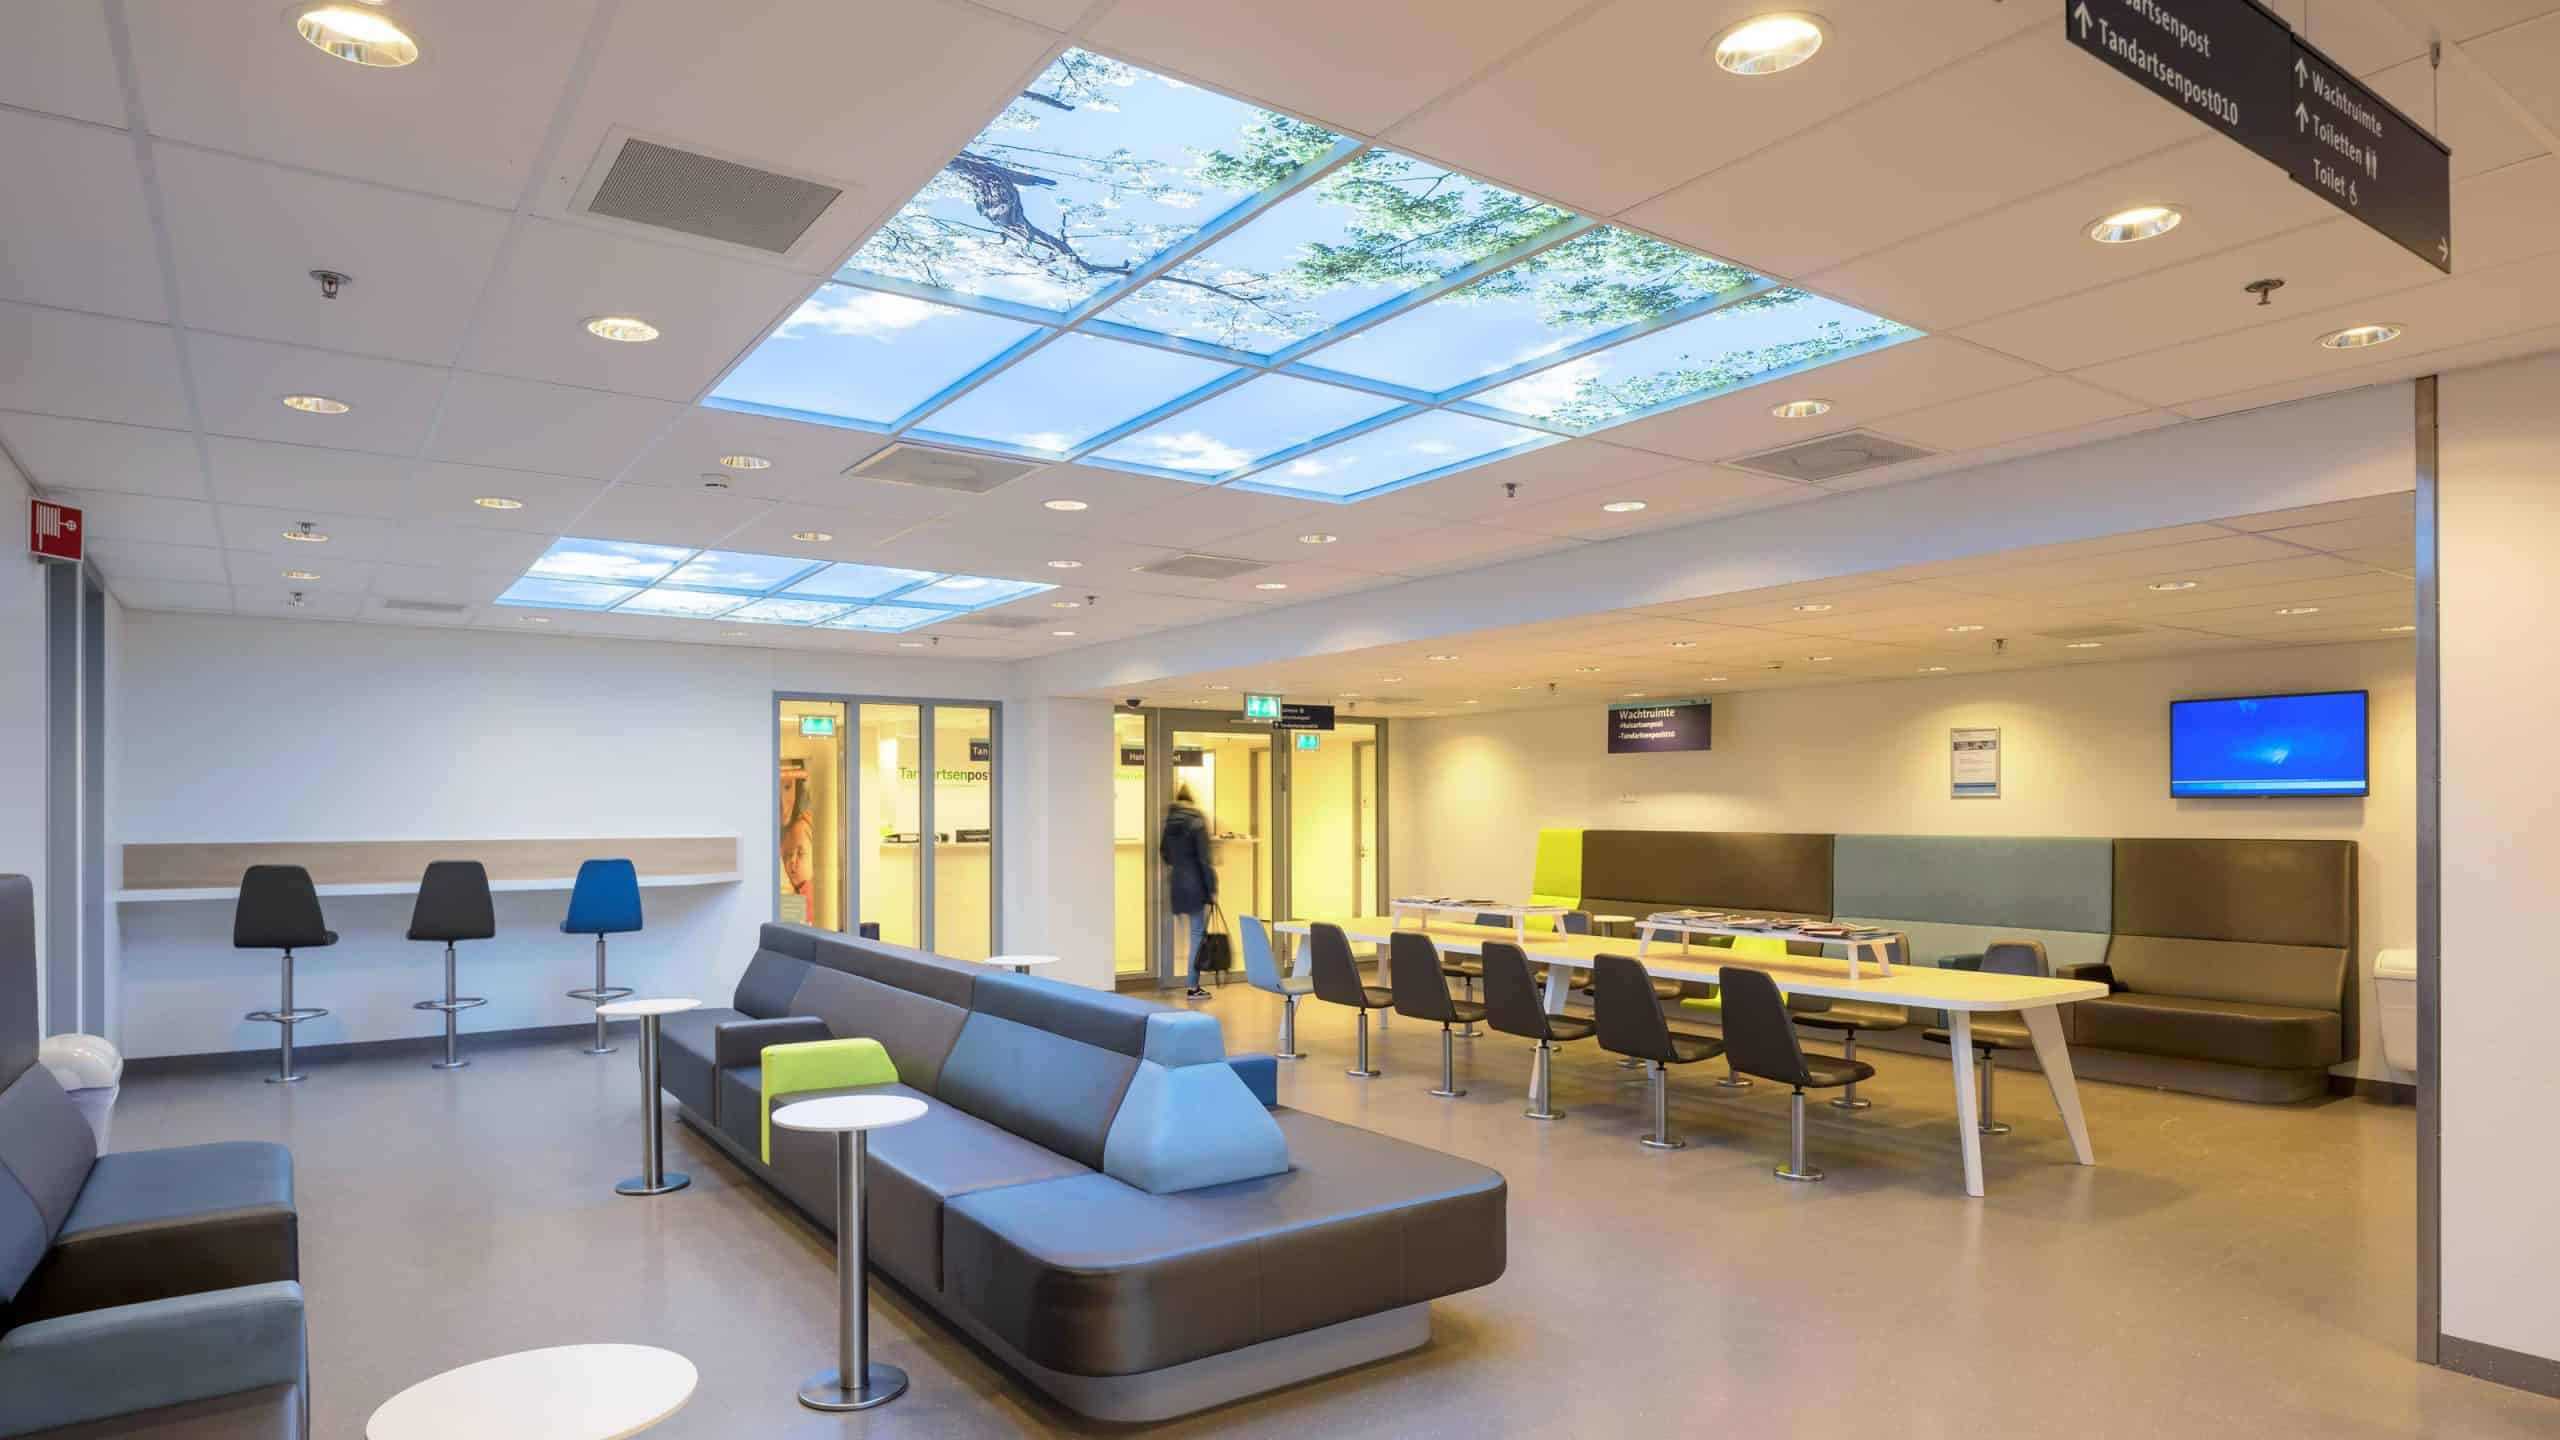
\includegraphics[width=8cm]{img/bp/ziekenhuis.jpg} \\ 
%        \hline
%        Type 2: Mutualiteit en verzekering & Another description for a second type, explaining its use case and characteristics. & 
%        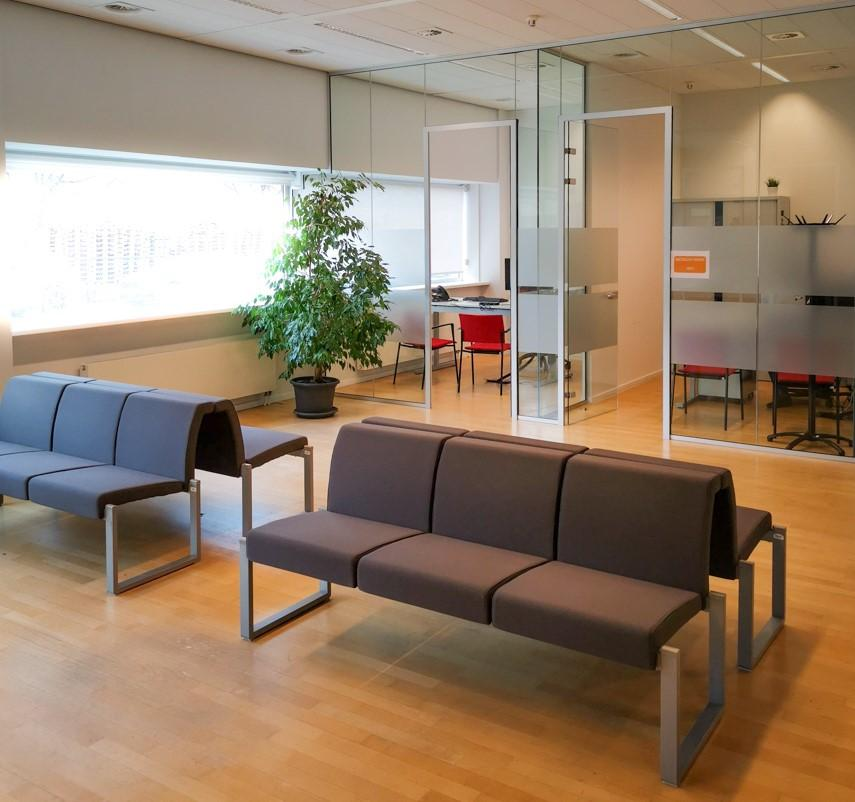
\includegraphics[width=8cm]{img/bp/mutualiteit.jpg} \\ 
%        \hline
%    \end{tabular}
%    \label{tab:type_description_image}
%\end{table}


% \section{Selectie van locatie}
% Om de Proof-of-Concept uit te voeren is de coöperatie van een medische instelling of andere sectoren noodzakelijk. Naast ziekenhuizen kunnen ook andere zorginstellingen in overweging worden genomen, zoals huisartspraktijken en Woonzorgcentra en Rusthuizen. % voor die reden wordt er naar een ziekenhuis gezocht die met voorkeur in Vlaanderen gelegen is. Het criteria bij het selecteren van een ziekenhuis is de geneigdheid van deze om samen te werken en de beschikbaarheid van de spoedafdeling om de Proof-of-Concept te kunnen uitvoeren. Tot slot moet de spoedafdeling beschikken over een wachtzaal met voldoende capaciteit voor patiënten en benodigde sensoren. 

%Voordat de Proof-of-Concept wordt uitgevoerd, wordt er een ziekenhuis gezocht, bij voorkeur in Vlaanderen. Een ziekenhuis wordt geselecteerd op basis van de bereidheid om samen te werken en de beschikbaarheid van een geschikte spoedafdeling voor het testen van het systeem. De spoedafdeling moet beschikken over een wachtzaal met voldoende capaciteit voor patiënten en benodigde sensoren. Om de samenwerking te vergemakkelijken, kan de Proof-of-Concept worden aangepast zodat deze volledig voldoet aan de geldende GDPR-richtlijnen van het ziekenhuis.
%\section{Locatieanalyse} \label{Locatieanalyse}
%Een grondige locatieanalyse zal uitgevoerd worden om een beter begrip te krijgen over de indeling van de spoedafdeling en wachtruimte. Deze controle wordt verricht om mogelijke obstakels te identificeren, zoals muren en andere structuren. Tijdens de inspectie zal de signaalsterkte gemeten worden door middel van een WiFi site survey software en zullen de toegangspunten voor stroom en netwerken gecontroleerd worden om de beste locatie voor de sensoren te identificeren. Hierbij zal er ook rekening gehouden worden met de locatie van de centrale eenheid en sensorcontroller. Een gedetailleerde kaart zal aangemaakt worden met de optimale locatie van de verschillende componenten. Het uiteindelijke doel van deze sectie is het identificeren van een locatie die de communicatie tussen de verschillende componenten efficiënt laat verlopen. 

\subsubsection{Devices}
De devices die in dit onderdeel worden besproken zijn geselecteerd op basis van de literatuurstudie en worden beschouwd als potentiële componenten voor het \gls{poc}. De uiteindelijke selectie van sensoren wordt beïnvloed door de specifieke topologie van de wachtruimte. Omdat het hier om een \gls{poc} gaat is er een beperkte controle over de indeling van de wachtruimte waardoor sommige sensoren mogelijk niet geplaatst kunnen worden.

\begin{itemize}
    \item Centrale eenheid
    \item Sensor controller
    \item Lichtsluis/\gls{ir}-sensor
    \item \gls{pir}-bewegingssensoren
    \item Ultrasoon/infraroodsensoren
\end{itemize}
\clearpage

%De reeds geïdentificeerde sensor- en subtypen in de literatuurstudie \ref{ch:stand-van-zaken} worden geanalyseerd en waar nodig aangevuld met aanvullende bronnen of nieuwe inzichten.

%Hierbij zal de huidige literatuurstudie \ref{ch:stand-van-zaken} gebruikt worden bij het analyseren van de reeds identificeerde devices

%daarom wordt er veel aandacht besteed bij het analyseren van de \gls{iot}-devices en gebruik hiervan in de gezondheidszorg

%\section{Plaatsingsstrategieën}
%Voor de plaatsing van de sensoren wordt er rekening gehouden met de sectie over plaatsingsstrategieën uit hoofdstuk \ref{ch:stand-van-zaken}. De keuze van de strategie zal afhangen van de resultaten uit de locatieanalyse \ref{Locatieanalyse} Eenmaal de nodige controles uitgevoerd worden de plaatsingsstrategieën uit hoofdstuk \ref{ch:stand-van-zaken} grondig geanalyseerd om de meeste gepaste strategie te implementeren, met als doel om nauwkeurige gegevens te verzamelen.

%\section{Software-identificatie}
%Het identificeren van de software is een belangrijke onderdeel bij het uitvoeren van de Proof-of-Concept. Software is nodig om \gls{iot} data te capteren, verwerken, analyseren, visualiseren, filteren en beveiligen. Hierbij is de identificatie van software voor elke stap van het proces essentieel. De identificatie gebeurt door het vaststellen van softwarecomponenten die deel uitmaken van het \gls{iot}-systeem. De software wordt geïdentificeerd door gebruik te maken van deze componenten het uitvoeren van een literatuurstudie. De software die hieruit komen worden verder vergeleken in een vergelijkingsstudie \ref{vergelijkingsoftware}.

%\subsection{Identificatie van softwarecomponenten} \label{softwarecomponenten}
%De softwarecomponenten hebben een essentiële rol bij het uitvoeren van de proof-of-concept. Daardoor wordt er aanzienlijk veel tijd besteed aan het identificeren hiervan. De identificatie gebeurt door een analyse van de Proof-of-Concept te realiseren, waarbij diverse componenten worden geïdentificeerd op basis van de benodigdheden van de Proof-of-Concept.

%\subsection{Softwarecomponenten} 
%Voor het identificeren van de softwarecomponenten worden specifieke onderdelen van de proof-of-concept geanalyseerd:

%\begin{table}[h]
%    \tiny
%    \caption{Tabel van de zin uit de \gls{poc} en de bijbehorende softwarecomponent}
%    \begin{tabular}{|p{10.5cm}|p{5cm}|}
%        \hline
%        \textbf{Zin uit \gls{poc}} & \textbf{Software Component} \\ \hline
%        De centrale eenheid of solution in de cloud verwerkt deze gegevens en berekent de volgorde en wachttijden van patiënten in de wachtruimte op basis van de tijdstempels. & Data Verwerking en Analyse \\ \hline
%        De data kan in real-time worden geanalyseerd om de wachttijden te berekenen en om te bepalen welke patiënt als volgende aan de beurt is. & Data Verwerking en Analyse \\ \hline
     %   Om de kans op false-positives en onnauwkeurige data te minimaliseren, worden technieken zoals filtering (om ruis te verminderen) en debouncing (om fluctuaties in digitale signalen te stabiliseren) toegepast op de sensorgegevens. & Debouncing en filtering van sensor data \\ \hline
        %Het dashboard zorgt ervoor dat het personeel gedetailleerde informatie kan raadplegen over de wachtruimte zoals het aantal patiënten, geschatte wachttijd per patiënt en volgorde van behandeling. & Dashboard en Visualisatie \\ \hline
        %De verzamelde data wordt vervolgens verstuurd door de sensor controller naar de centrale eenheid via een seriële verbinding of draadloze protocol & Netwerk en communicatieprotocol \\ \hline
%        Een thermische camera zal tot slot gebruikt worden om staande patiënten te detecteren & Integratie voor een thermische camera \\ \hline
        %Aangezien dat \gls{iot}-technologieën diverse beveiligings- en ethische risico's met zich meebrengen worden er verschillende beveiligings- en ethische maatregelen geïmplementeerd zelfs als er geen persoonlijke gegevens verzameld worden. & Gegevensbeveiliging \\ \hline
%    \end{tabular}
%    \label{tab:zin_software}
%\end{table}

%\begin{itemize}
    %\item \textbf{\gls{iot} Hardware-software:} Software voor het beheren van de sensoren die de beweging en aanwezigheid van patiënten detecteren.
%    \item \textbf{Data Verwerking en Analyse:} Voor het verwerken van sensorgegevens en het analyseren hiervan.
    %\item \textbf{Dashboard en Visualisatie:} Software voor het visualiseren van de verwerkte gegevens.
    %\item \textbf{Debouncing en filtering van sensor data:} Software voor het verminderen van ruis en stabiliseren van digitale signalen.
    %\item \textbf{Netwerk en communicatieprotocol:} Software voor de communicatie tussen de sensoren, sensorcontroller en centrale eenheid.
    %\item \textbf{Gegevensbeveiliging:} Software voor mogelijke gegevensbeveiliging indien nodig.
%    \item \textbf{Integratie voor een thermische camera} Software voor de integratie van een thermische camera.
%\end{itemize}

%Na het identificeren van de software worden deze voor elke implementatie met elkaar vergeleken in een vergelijkende studie \ref{vergelijkendeanalyse}.

%\section{Identificatie van een cloud oplossing} \label{cloud}
%Bij het uitvoeren van de Proof-of-Concept zal er gebruik gemaakt worden van een cloudgebaseerd platform. Hierop zal een software draaien die verantwoordelijk is voor het analyseren van de binnenkomende data en de wachttijden berekenen. Net zoals bij de selectie van \gls{iot} devices en identificeren van software zal er gebruik gemaakt worden van een vergelijkende studie waarbij diverse cloud oplossingen vergeleken worden op basis van de volgende kenmerken

%\section{Case study}
%Deze case study heeft als hoofddoel het verklaren van de implementatie van \gls{iot} technologieën door het identificeren van concrete voorbeelden van \gls{iot}-gebruik bij het verminderen van wachttijden op A\&E afdelingen. De case study richt zich verder op het vaststellen van \gls{iot} apparaten die ingezet kunnen worden om wachttijden te verkorten. De case study begint met het identificeren van specifieke casussen. Hiervoor worden verschillende bronnen geraadpleegd (Academische artikelen, Boeken, Wetenschappelijke artikelen, enzovoort) met als doel om kwalitatieve en kwantitatieve gegevens te verzamelen. De \gls{iot}-devices en categorieën die voorkomen in de casussen worden verder opgelijst en geanalyseerd. Tot slot worden verschillende bronnen geraadpleegd bij het verzamelen van gegevens voor iedere identificeerde \gls{iot}-device. Deze gegevens zullen verder in de volgende fase gebruikt worden.

%Deze case study wordt uitgevoerd als toelichting voor het implementeren van \gls{iot} technologieën. De primaire doelstelling van deze case study is het identificeren van praktische voorbeelden van \gls{iot} gebruik om lange wachttijden in A\&E afdelingen te verminderen. Daarnaast richt de case study zich op het identificeren van verschillende \gls{iot} apparaten die ingezet kunnen worden om wachttijden verder te verkorten. De case study begint met het identificeren van specifieke casussen. Na het vaststellen van een casus worden er kwalitatieve en kwantitatieve gegevens verzameld over de gekozen casus, dit houdt in dat verschillende bronnen worden geraadpleegd bij het verzamelen van informatie zoals wetenschappelijke literatuur, rapporten van gezondheidsorganisaties, archieven en documenten. Na het vaststellen van diverse casussen worden deze geanalyseerd en de gebruikte \gls{iot}-devices en \gls{iot} categorieën opgelijst. Verder worden gegevens verzameld voor elk van de opgelijste devices, verschillende bronnen zoals onderzoeksrapporten, literatuurstudies, academische tijdschriften en technologische onderzoeken worden hiervoor geraadpleegd. 

%\section{Identificeren van \gls{iot}-devices}
%Het identificeren van \gls{iot}-devices is een essentiële fase in deze studie, daarom wordt er veel aandacht besteed bij het uitwerken van de case study en bijgevolg het identificeren van \gls{iot}-devices. Deze devices worden geselecteerd op basis van de categorie waartoe ze behoren. De categorieën worden bepaald volgens de benodigdheden in van de proof-of-concept. Elke device die tot een categorie behoort wordt grondig bestudeerd om beter te begrijpen hoe deze werkt en geïmplementeerd kan worden in de proof-of-concept. \ASK

%Het identificeren van \gls{iot} apparaten is van het uiterste belang, daarom is er aanzienlijk veel tijd besteed aan het opstellen van de casestudie om een assortiment van \gls{iot} apparaten te bepalen. Dit houdt in dat elk device grondig bestudeerd zal worden om een beter begrip te krijgen in de werking hiervan in de gezondheidszorg. Om het meest gepaste \gls{iot} device te selecteren worden verschillende \gls{iot} categorieën bekeken, deze categorieën vertegenwoordigen \gls{iot} apparaten die de werking van de A\&E afdelingen kunnen verbeteren en efficiënter maken, deze categorieën zijn: Locatie- en traceerapparaten, Communicatieapparaten, Integratie van het gegevensbeheer en Integratie en coördinatie van \gls{iot} devices. De categorieën worden geselecteerd op basis van de nodige \gls{iot} devices in de proof-of-concept. Het Real-time Smart Queue Management System maakt gebruik van bewegings- en aanwezigheidssensoren, die worden ingezet om de locatie van patiënten in de wachtrij in real-time te volgen.

\subsubsection{Methodologie van vergelijking}

De vergelijkende studie bevat de volgende criteriums:
\begin{itemize}
    \item \textbf{Centrale eenheid en sensor controller}
    \begin{itemize}
        \item Voor- en nadelen: Een overzicht van de voordelen en nadelen van deze twee componenten.
        \item Kosten: omvat enkel de aanschafkosten van deze onderdelen.  
    \end{itemize}
    
    \item \textbf{Vergelijking van sensoren}
    Een selectie van sensoren per type wordt met elkaar vergeleken:
    \begin{itemize}
        \item Lichtsluis-/Infraroodsensoren
        \item \gls{pir}-bewegingssensoren
        \item Ultrasoon sensoren
    \end{itemize}
    
    De vergelijking gebeurt op basis van de volgende criteria:
    \begin{itemize}
        \item Nauwkeurigheid
        \item Gevoeligheid
        \item Bereik
        \item Connectiviteit
        \item Kostprijs (€)
    \end{itemize}
\end{itemize}


\subsubsection{Vergelijking van devices}

\begin{table}[h!]
    \small
    \caption{Vergelijking van Centrale Eenheden voor \gls{iot} \autocite{Calvo2016, Hosny2023, SainzRaso2019, 王丁2014, Pham2024}}
    \label{tab:vergelijking-centrale-eenheid}
    \begin{tabular}{|p{2cm}|p{3.8cm}|p{4cm}|p{4cm}|}
        \hline
        \textbf{Criteria} & \textbf{Raspberry Pi 4 8GB} & \textbf{HP EliteDesk 800 G3 USFF} & \textbf{NVIDIA Jetson Nano} \\
        \hline
        \textbf{Voordelen} & Betaalbaar, algemeen ondersteund, ideaal voor kleinere \gls{iot}-projecten & Compact en energie-efficiënt design, geschikt voor kleine ruimtes & Krachtig voor real-time verwerking, energiezuinig, ideaal voor mobiele toepassingen \\
        \hline
        \textbf{Nadelen} & Beperkingen in CPU, RAM, kwetsbaar door afhankelijkheid van software en OS & Beperkingen in rekenkracht, problemen met koeling en connectiviteit & Beperkingen in geheugen en rekenkracht voor grotere AI-modellen, niet geschikt voor zware GPU-taken  \\
        \hline
        \textbf{Kost (€)} & €75 (reeds in bezit) & €99,00 & €200-300 \\
        \hline
    \end{tabular}
\end{table}
\clearpage

%---------------------------------------------------------------------------------------------

\begin{table}[h!]
    \small
    \caption{Vergelijking van Sensor Controllers \autocite{Hussain2024, Viriyavisuthisakul2017, Spohn2020, Maier2017, Wang2020, Wu2020, Kovacshazy2024}}
    \label{tab:vergelijking-sensorcontroller}
    \begin{tabular}{|p{2cm}|p{4cm}|p{4cm}|p{4cm}|}
        \hline
        \textbf{Criteria} & \textbf{Arduino Nano 33 \gls{iot}} & \textbf{ESP32-WROOM} & \textbf{STM32} \\
        \hline
        \textbf{Voordelen} 
        & Kosteneffectief en kan ingezet worden om wachtrijlengtes te detecteren en personeel te waarschuwen. 
        & Efficiënt voor \gls{iot} met laag verbruik, dual-core en WiFi/Bluetooth. 
        & Hoge performantie en energie-efficiëntie in uiteenlopende \gls{iot}-toepassingen. \\
        \hline
        \textbf{Nadelen} 
        & Beperkte kracht en geen RTOS, lastig voor complexe toepassingen. 
        & Lagere performantie bij hoge zendfrequenties en druk WiFi-netwerk. 
        & Uitdagingen bij toepassingen met hoge verwerkingsvereisten en complexe connectiviteit. \\
        \hline
        \textbf{Kost (€)} 
        & €28,07 
        & €19,95 
        & €24,13 \\
        \hline
    \end{tabular}
\end{table}

%----------------------------------------------------------------------------------------------
\begin{table}[h!]
    \small
    \caption{Vergelijking van lichtsluis-infraroodsensoren \autocite{Industries2024, Omron2024, KEYENCE}}
    \begin{tabular}{|p{3cm}|p{4cm}|p{3.5cm}|p{3.5cm}|} % <-- extra | tussen kolom 2 en 3
        \hline
        \textbf{Criteria} & \textbf{Adafruit Infrared Break Beam (5mm)} & \textbf{Omron E3Z-T61} & \textbf{Keyence PZ-G51N} \\
        \hline
        Meetmethode & Lichtsluis met onderbrekingsdetectie via infrarood & Lichtsluis met infrarood onderbrekingsdetectie & Reflecterende fotocel met objectdetectie via infrarood \\
        \hline
        Bereik & 50 cm & 15 m & 20 m \\
        \hline
        Kost (€) & €2,52 & €36,29 & €73,95 \\
        \hline
    \end{tabular}
\end{table}

%----------------------------------------------------------------------------------------------
\begin{table}[h!]
    \small
    \caption{Vergelijking van \gls{pir}-bewegingssensoren \autocite{LastMinuteEngineersa, HobbyComponents, LastMinuteEngineers}}
    \label{tab:vergelijking-thermische-camera}
    \begin{tabular}{|p{4cm}|p{3.5cm}|p{3.5cm}|p{3cm}|}
        \hline
        \textbf{Criterium} & \textbf{HC-SR501} & \textbf{AM312} & \textbf{RCWL-0516} \\
        \hline
        Bereik & 7 meter & 3 meter & 5-7 meter \\
        \hline
        Detectiehoek & 120° & <100° & 360° \\
        \hline
        Kost (€) & €5,95 & €1,49 & €1.80 \\
        \hline
    \end{tabular}
\end{table}
\clearpage

%----------------------------------------------------------------------------------------------
\begin{table}[h!]
    \small
    \caption{Vergelijking van ultrasone sensoren \autocite{Elecfreaks2025, Inc.2025, Inc.2025a}}
    \label{tab:vergelijking-ultrasoonsensoren}
    \begin{tabular}{|p{3.5cm}|p{3cm}|p{3.5cm}|p{4cm}|}
        \hline
        \textbf{Criterium} & \textbf{HC-SR04} & \textbf{Parallax Inc PING} & \textbf{MB1240 XL-MaxSonar-EZ4} \\
    \hline
    Bereik & 2 cm – 4 m & 2 cm – 3 m & 20 cm – 7 m \\
    \hline
    Nauwkeurigheid & ±0.3 cm & ±1 cm & ±1 cm (typisch) \\
    \hline
    Voedingsspanning & 5 V & 5 V & 3.3–5 V \\
    \hline
    Kosten (€)* & €2,10 & €33,11 & €29,95 \\
    \hline
\end{tabular}
\end{table}


\subsubsection{Conclusie vergelijkende studie}
Volgens de bevindingen uit de vergelijkende studie worden de volgende devices geselecteerd. De devices die werkelijk gebruikt zullen worden zal bepaald worden in het \gls{poc}.

\begin{table}[h!]
    \small
    \renewcommand{\arraystretch}{1.2}
    \caption{Geselecteerde \gls{iot} Devices}
    \begin{tabular}{|l|c|p{8cm}|}
        \hline
        \textbf{\gls{iot} Device} & \textbf{Price (EUR)} & \textbf{Reason of Choice} \\
        \hline
        Raspberry Pi & IN BEZIT & Reeds in bezit, veelzijdig voor prototyping. De beveiligingsnadelen zijn voor het \gls{poc} minder van belang.\\
        \hline
        ESP32-WROOM & €19,95  & Kost, Laag energieverbruikt, dual-core en Wi-Fi Bluetooth support. \\
        \hline
        Adafruit \gls{ir} Break Beam & €2,52 & Zeer goedkoop, voldoende bereik (50 cm) voor deuropeningen of smalle doorgangen. Makkelijk te integreren.
         \\
        \hline
        HC-SR501 & €5,95  & Goede balans tussen bereik (7 m), brede detectiehoek (120°), en lage kostprijs. Bewezen sensor in veel projecten. \\
        \hline
        HC-SR04 & €2,10  & Zeer lage prijs, voldoende nauwkeurigheid en bereik voor wachtruimtedetectie. \\    
    \end{tabular}
    \begin{tabular}{|p{4.17cm}|p{10.5cm}|}
    \hline
    \textbf{Total} & \textbf{€83,18} \\
    \hline
    \end{tabular}
    \label{tab:iot_prices}
\end{table}}
\clearpage

%--------------------------------------------------------------------------------------------
%\subsection{Vergelijkende studie: Cloudgebaseerde platform}
\TODO


%--------------------------------------------------------------------------------------------
%\subsection{Vergelijkende studie: Software componenten} \label{vergelijkingsoftware}
%In deze sectie worden verschillende software componenten met elkaar vergeleken om de meest geschikte keuze te maken voor de Proof-of-Concept. De resultaten van deze vergelijking leiden tot een aanbeveling voor de meest geschikte softwarecomponent voor de Proof-of-Concept. Deze aanbeveling wordt ondersteund door een uitgebreide uitleg van waarom bepaalde software de voorkeur krijgen boven andere, met speciale aandacht voor hoe ze bijdragen aan de doelstellingen van het project.

%\subsubsection{Keuze methodologie van vergelijking}
%Voor een objectieve vergelijking wordt diverse vergelijkingsmethodologieën onderzocht, hiervoor worden verschillende website(s) geraadpleegd zoals wetenschappelijke studies en onafhankelijke reviewplatformen zoals Gartner, Capterra en Trustradius. Daarnaast worden academische studies geanalyseerd om de meest gepaste methode te selecteren voor elke criteria. Een methodologie wordt verder geselecteerd op basis van de soort van gegeven (kwantitatief, kwalitatief).

%\subsubsection{Inhoud vergelijkende studie: Softwarecomponenten}
%De softwarecomponenten die vergeleken worden zijn benoemd onder sectie \ref{softwarecomponenten} \textit{Identificatie van software componenten}. 

%\subsubsection{Vergelijkingscriteria}
%Om een duidelijke beeld te krijgen over de meest geschikte software worden deze op diverse kwantitatieve en kwalitatieve criteria vergeleken. Deze criteriums dekken belangrijke aspecten van zowel de technische en operationele kant van softwaretoepassingen.

%\begin{itemize}
%    \item \textbf{Kosten:} De kostenanalyse omvat zowel de licentiekosten als eventuele implementatie- en onderhoudskosten, voor de implementatiekosten wordt er rekening gehouden met kosten voor cloudgebaseerd platformen. \TODO
%    \item \textbf{Betrouwbaarheid:} De stabiliteit van de software wordt geëvalueerd op basis van throughput, Latency en fault tolerance.
%    \item \textbf{Ondersteuning en community:} De beschikbaarheid van documentatie en ondersteuning. 
%    \item \textbf{Gebruiksvriendelijkheid:} Dit criterium omvat de eenvoud van installatie, configuratie en het gebruik van de software.
%    \item \textbf{Integratiemogelijkheden:} De mogelijkheid om de softwarecomponent te integreren met andere systemen of platforms (zoals databases, \gls{iot}-apparaten, API’s) wordt onderzocht. 
%\end{itemize}

%\subsubsection{Vergelijkingsmethodologieën}

%\begin{table}[h]
%    \caption{Overzicht van methodologieën per criterium}
%    \centering
%    \tiny
%    \renewcommand{\arraystretch}{1.3}
%    \begin{tabular}{|p{4cm}|p{5cm}|p{6cm}|}
%        \hline
%        \textbf{Criterium} & \textbf{Methodologie} & \textbf{Toelichting} \\ \hline
%        Kosten & TCO-analyse (Total Cost of Ownership) & Vergelijking van licentie, hostingkosten. \\ \hline
%        Betrouwbaarheid & Empirische analyse + SLA-analyse & Betrouwbaarheid wordt gemeten met historische gegevens, statistieken en Service Level Agreements (SLA) \\ \hline
%        Ondersteuning en community & Benchmarking & Vergelijk, responsiviteit van de community en beschikbaarheid van technische ondersteuning. \\ \hline
%        Gebruiksvriendelijkheid & Usability Testing & Uittesten van de software en beoordeel op basis van gebruiksvriendelijkheid. \\ \hline
%        Integratiemogelijkheden & Feature-matching + API-documentatieanalyse & Onderzoek compatibiliteit met andere systemen en de flexibiliteit van API’s. \\ \hline
%    \end{tabular}
%    \label{tab:methodologieen}
%\end{table}


%\subsubsection{Vergelijking van softwarecomponenten}

%\paragraph{Kosten}
%\TODO

%\paragraph{Betrouwbaarheid}
%De betrouwbaarheid wordt gemeten dankzij een empirische- en SLA analyse. De meting wordt uitgevoerd op basis van de volgende metrieken: 

%\begin{table}[ht]
%    \tiny
%    \caption{Evaluatie van de stabiliteit van de software, \autocite{Padmanaban2024, Raza2021, Singh2022, Rinaldi2019, Mehdi2023, Chakraborty2021, Rajput2024}}
%    \renewcommand{\arraystretch}{1.5} % Verhoog de rijhoogte voor meer ruimte
%    \begin{tabular}{|l|l|p{5cm}|p{4cm}|p{4cm}|} % Extra kolom voor categorie
%        \hline
%        \textbf{Categorie} & \textbf{Software} & \textbf{Throughput} & \textbf{Latency} & \textbf{Fault tolerance} \\
%        \hline
%        Verwerking & Apache Kafka & 750-1340 events per uur. & 6-15 milliseconden & Er bestaat fout tolerantie voor netwerk problemen maar er zijn tekorten.  \\
%        \hline
%        Analyse & Apache Flink & +1 miljoen events per seconde & 2.5-2.7 milliseconden voor complexe queries & Heeft een robuuste fouttolerantie, deze heeft een impact op de performantie maar is essentieel voor de betrouwbaarheid.  \\
%        \hline
%        Verwerking & InfluxDB & Kan variëren van millisecondes naar secondes volgens de data model. & 3.374 milliseconden & Er bestaat fout tolerantie. \\
%        \hline
%        \textbf{Categorie} & \textbf{Software} & \textbf{Ease of use} & \textbf{Best for} & \textbf{Data Connectivity} \\
%        \hline
%        Monitoring & Grafana & Gebruiksvriendelijk interface maakt het gebruik makkelijk voor gebruikers met verschillende technische achtergronden. Dit maakt het configureren, aanpassen en visualiseren makkelijk  & Real-time monitoring en visualiseren van data uit verschillende bronnen. Grafana is uitstekend bij het creëren van interactieve aanpasbare dashboards dat data van servers, databases en \gls{iot} devices integreert. & Ondersteunt diverse time-series en SQL-databases. \\
%        \hline
%        Monitoring & Power Bi & Gebruikersvriendelijk dankzij zijn drag-and-drop interface & N/A & N/A \\
%        \hline
%        Monitoring & Tableau & De bevindingen tonen de snelheid en effectiviteit van de technische ondersteuning bij het oplossen van problemen, met een gemiddelde oplostijd van 4 uur. & N/A & N/A \\
%        \hline
%    \end{tabular}
%\end{table}


%\subsubsection{Resultaten en Discussie}

%\subsubsection{Conclusie en aanbevelingen}
%-----------------------------------------------------------------------------------------------

\section{Procedure: \gls{poc}} \TODO % Maak een lijst met alle afkortingen
De Proof-of-Concept (\gls{poc}) richt zich op het onderzoeken hoe \gls{iot} ingezet kan worden om wachttijden inzichtelijk te maken en duidelijk weer te geven. Dit vormt een basis voor toekomstige optimalisaties. Het doel is niet om tijdens de meetperiode direct een afname van wachttijden te realiseren. \\

Het is belangrijk om te benadrukken dat de werking van het \gls{iot}-systeem binnen deze \gls{poc} experimenteel is. Het systeem bevindt zich in een testfase, waarbij de prestaties kunnen afwijken door sensorinstellingen, netwerkverbinding en omgevingsomstandigheden. Hierdoor kan het voorkomen dat tijdens de meetperiode niet alle data volledig of bruikbaar zijn. \\

Toch biedt deze opzet waardevolle inzichten in de haalbaarheid en aandachtspunten bij het implementeren van een \gls{iot}-gebaseerd meetsysteem voor bezettingsinformatie.

\subsection{Voorbereidende fase}
Het \gls{poc} werd uitgevoerd in samenwerking met \gls{wgc} De Vlier, een eerstelijnsgezondheidscentrum waar wachttijden en ruimtegebruik belangrijke aandachtspunten vormen. \\

Voor de opbouw van het meetsysteem werd vooraf een plaatsbezoek uitgevoerd om de wachtruimte in kaart te brengen. Hierbij werd de wachtruimte geanalyseerd op:

\begin{itemize}
    \item Afmetingen van de ruimte en deuropeningen
    \item Positie en afstand tussen stoelen
    \item Beschikbare stroompunten en Wi-Fi-dekking
    \item Mogelijke reflecterende oppervlakken die sensormetingen kunnen beïnvloeden
    \item Verwachte bezoekersstromen en typische gedragingen (staan, zitten, rondlopen)
\end{itemize}

%De fotodocumentatie bestaat uit:
%\begin{itemize}
%    \item Ingang(en) en doorgangen waar break beam sensoren worden geplaatst
%    \item Zithoeken voor de detectie via \gls{pir}- en ultrasone sensoren
%    \item Plafondzones geschikt voor sensorbevestiging
%    \item Overzicht van de ruimte voor validatie van sensorbereik en -plaatsing
%\end{itemize}

%De foto's zijn terug te vinden in Bijlage B en worden gebruikt als visuele onderbouwing van de gekozen sensorconfiguratie en meetzones.

\subsection{Nulmeting en verzameling van historische gegevens}
Om de effectiviteit van het \gls{poc} te evalueren, werd een nulmeting uitgevoerd met Google Vertex AI Occupancy Analytics. Deze meting vond plaats gedurende 4 dagen tijdens de openingsuren (08:00 tot 19:00) in de wachtruimte van \gls{wgc} De Vlier. \\

Tijdens deze nulmeting werden gegevens verzameld zoals het aantal aanwezige personen per minuut. Deze meting vormt een praktisch referentiepunt waarmee achteraf de prestaties van het \gls{iot}-gebaseerde meetsysteem vergeleken kunnen worden. \\

Hoewel deze AI-gebaseerde meting als nulmeting wordt gepresenteerd, is het belangrijk te benadrukken dat dit geen absolute waarheid is. Omdat de bezetting in de wachtruimte zelden hoger ligt dan drie à vier personen, kunnen zelfs kleine afwijkingen (zoals dubbeltellingen of detectievertragingen) een relatief grote invloed hebben op de gemeten waarden. 

\subsubsection{Duur van de nulmeting en motivatie}
Tijdens 4 dagen werden de bezettingsgegevens per minuut geregistreerd. Dit resulteerde in een totaal van ongeveer 1.756 meetmomenten. De nulmeting duurde 4 dagen omdat de maandag in die week een feestdag was. Zo bleef de planning op schema. De meetperiode werd bewust kort gehouden vanwege privacybezwaren bij \gls{wgc} De Vlier. Om die reden werd gekozen voor een korte, representatieve meetperiode die piek- en dalmomenten omvat. Op die manier kon de nulmeting voldoende variatie capteren in bezoekersaantallen zonder de vertrouwelijkheid of het comfort van patiënten langdurig te schaden.

\subsubsection{Selectie en configuratie van de \gls{rtsp}-camera voor de nulmeting}
Voor het uitvoeren van de nulmeting met Google Vertex AI Occupancy Analytics dient er een \gls{rtsp}-compatibele camera geselecteerd te worden, dit is een essentieel onderdeel om de bezetting binnen de wachtruimte in realtime te monitoren. Het beeld wordt vervolgens gekoppeld met Google Vertex AI Occupancy Analytics via een \gls{rtsp}-stream. \\

De keuze van een \gls{rtsp}-camera komt door het feit dat deze in staat is om live te streamen naar een server, applicatie of AI-dienst zoals Google Vertex AI Vision. Hierdoor kan de bezettingsgraad geanalyseerd worden zonder beelden op te slaan. \\

\textbf{Selectiecriteria voor de camera}
\begin{itemize}
    \item Ondersteuning voor \gls{rtsp}
    \item Minimale resolutie van 720p
    \item Groothoeklens voor maximale dekking
    \item Geen lokale opslag vereist
    \item Geen montage met schroeven vereist
\end{itemize}
  
\textbf{Vergelijking camera's} \\
Volgens de selectiecriteria wordt er een keuze gemaakt uit de volgende camera's, deze werden gekozen op basis van de prijs en voor- en nadelen.
\begin{table}[h!]
    \centering
    \caption{\gls{rtsp}-camera's}
    \begin{tabular}{|p{3.5cm}|p{1.8cm}|p{6cm}|p{3cm}|}
        \hline
        \textbf{Camera} & \textbf{Prijs (€)} & \textbf{Voordelen} & \textbf{Nadelen} \\
        \hline
        Reolink E1 Zoom & ± €60 & Ondersteunt \gls{rtsp}; 2K resolutie; Draaibaar via app; Staat stabiel op vlak oppervlak; Wi-Fi verbinding & Geen PoE-ondersteuning \\
        \hline
        TP-Link Tapo C210 & ± €40 & 2K resolutie; \gls{rtsp} in te schakelen via instellingen; Compact en vrijstaand; Draaibaar via app & \gls{rtsp} vereist manuele activatie \\
        \hline
        Amcrest IP2M-841 & ± €70 & Native \gls{rtsp} en ONVIF; Geschikt voor AI-analyse; Tafelmodel, geen montage nodig & Groter formaat \\
        \hline
        Wyze Cam v3 & ± €35 & Budgetvriendelijk; Compact en eenvoudig te plaatsen; \gls{rtsp} beschikbaar via alternatieve firmware & \gls{rtsp} niet standaard; Vereist aparte firmware-installatie \\
        \hline
    \end{tabular}
    \label{tab:rtsp-cams}
\end{table}


\textbf{Geselecteerde camera voor nulmeting} \\
Volgens de vergelijking is de \textit{Reolink E1 Zoom} de beste keuze omdat het \gls{rtsp} ondersteunt, zonder boorwerk geïnstalleerd kan worden, een hoge beeldkwaliteit biedt en vlot integreert met Google Vertex AI Occupancy Analytics. Het enige nadeel is dat deze camera duurder is vergeleken met de andere camera's maar het is het waard om een kwalitatieve meting uit te voeren.

\subsubsection{Vision-gebaseerde nulmeting via Vertex AI en Reolink E1 Zoom}
De nulmeting was de eerste stap van het \gls{poc} om een referentie te verkrijgen van de bezettingsgraad in de wachtruimte. De meting gebeurde via een vision-gebaseerde aanpak, waarbij gebruik werd gemaakt van de Reolink E1 Zoom-camera in combinatie met Google Vertex AI Vision. \\

De camera werd zonder montage op een kast in de hoek van de wachtruimte geplaatst en dankzij de draaibare lens was de volledige ruimte zichtbaar. Via \gls{rtsp}-streaming werd het videobeeld in realtime doorgestuurd naar de cloudomgeving van Vertex AI Vision, waar een AI-gebaseerd model (Occupancy analytics) personen detecteerde en telde. \\

\begin{figure}[h!]
    \centering
    % Eerste rij met twee afbeeldingen
    \begin{minipage}[b]{0.49\textwidth}
        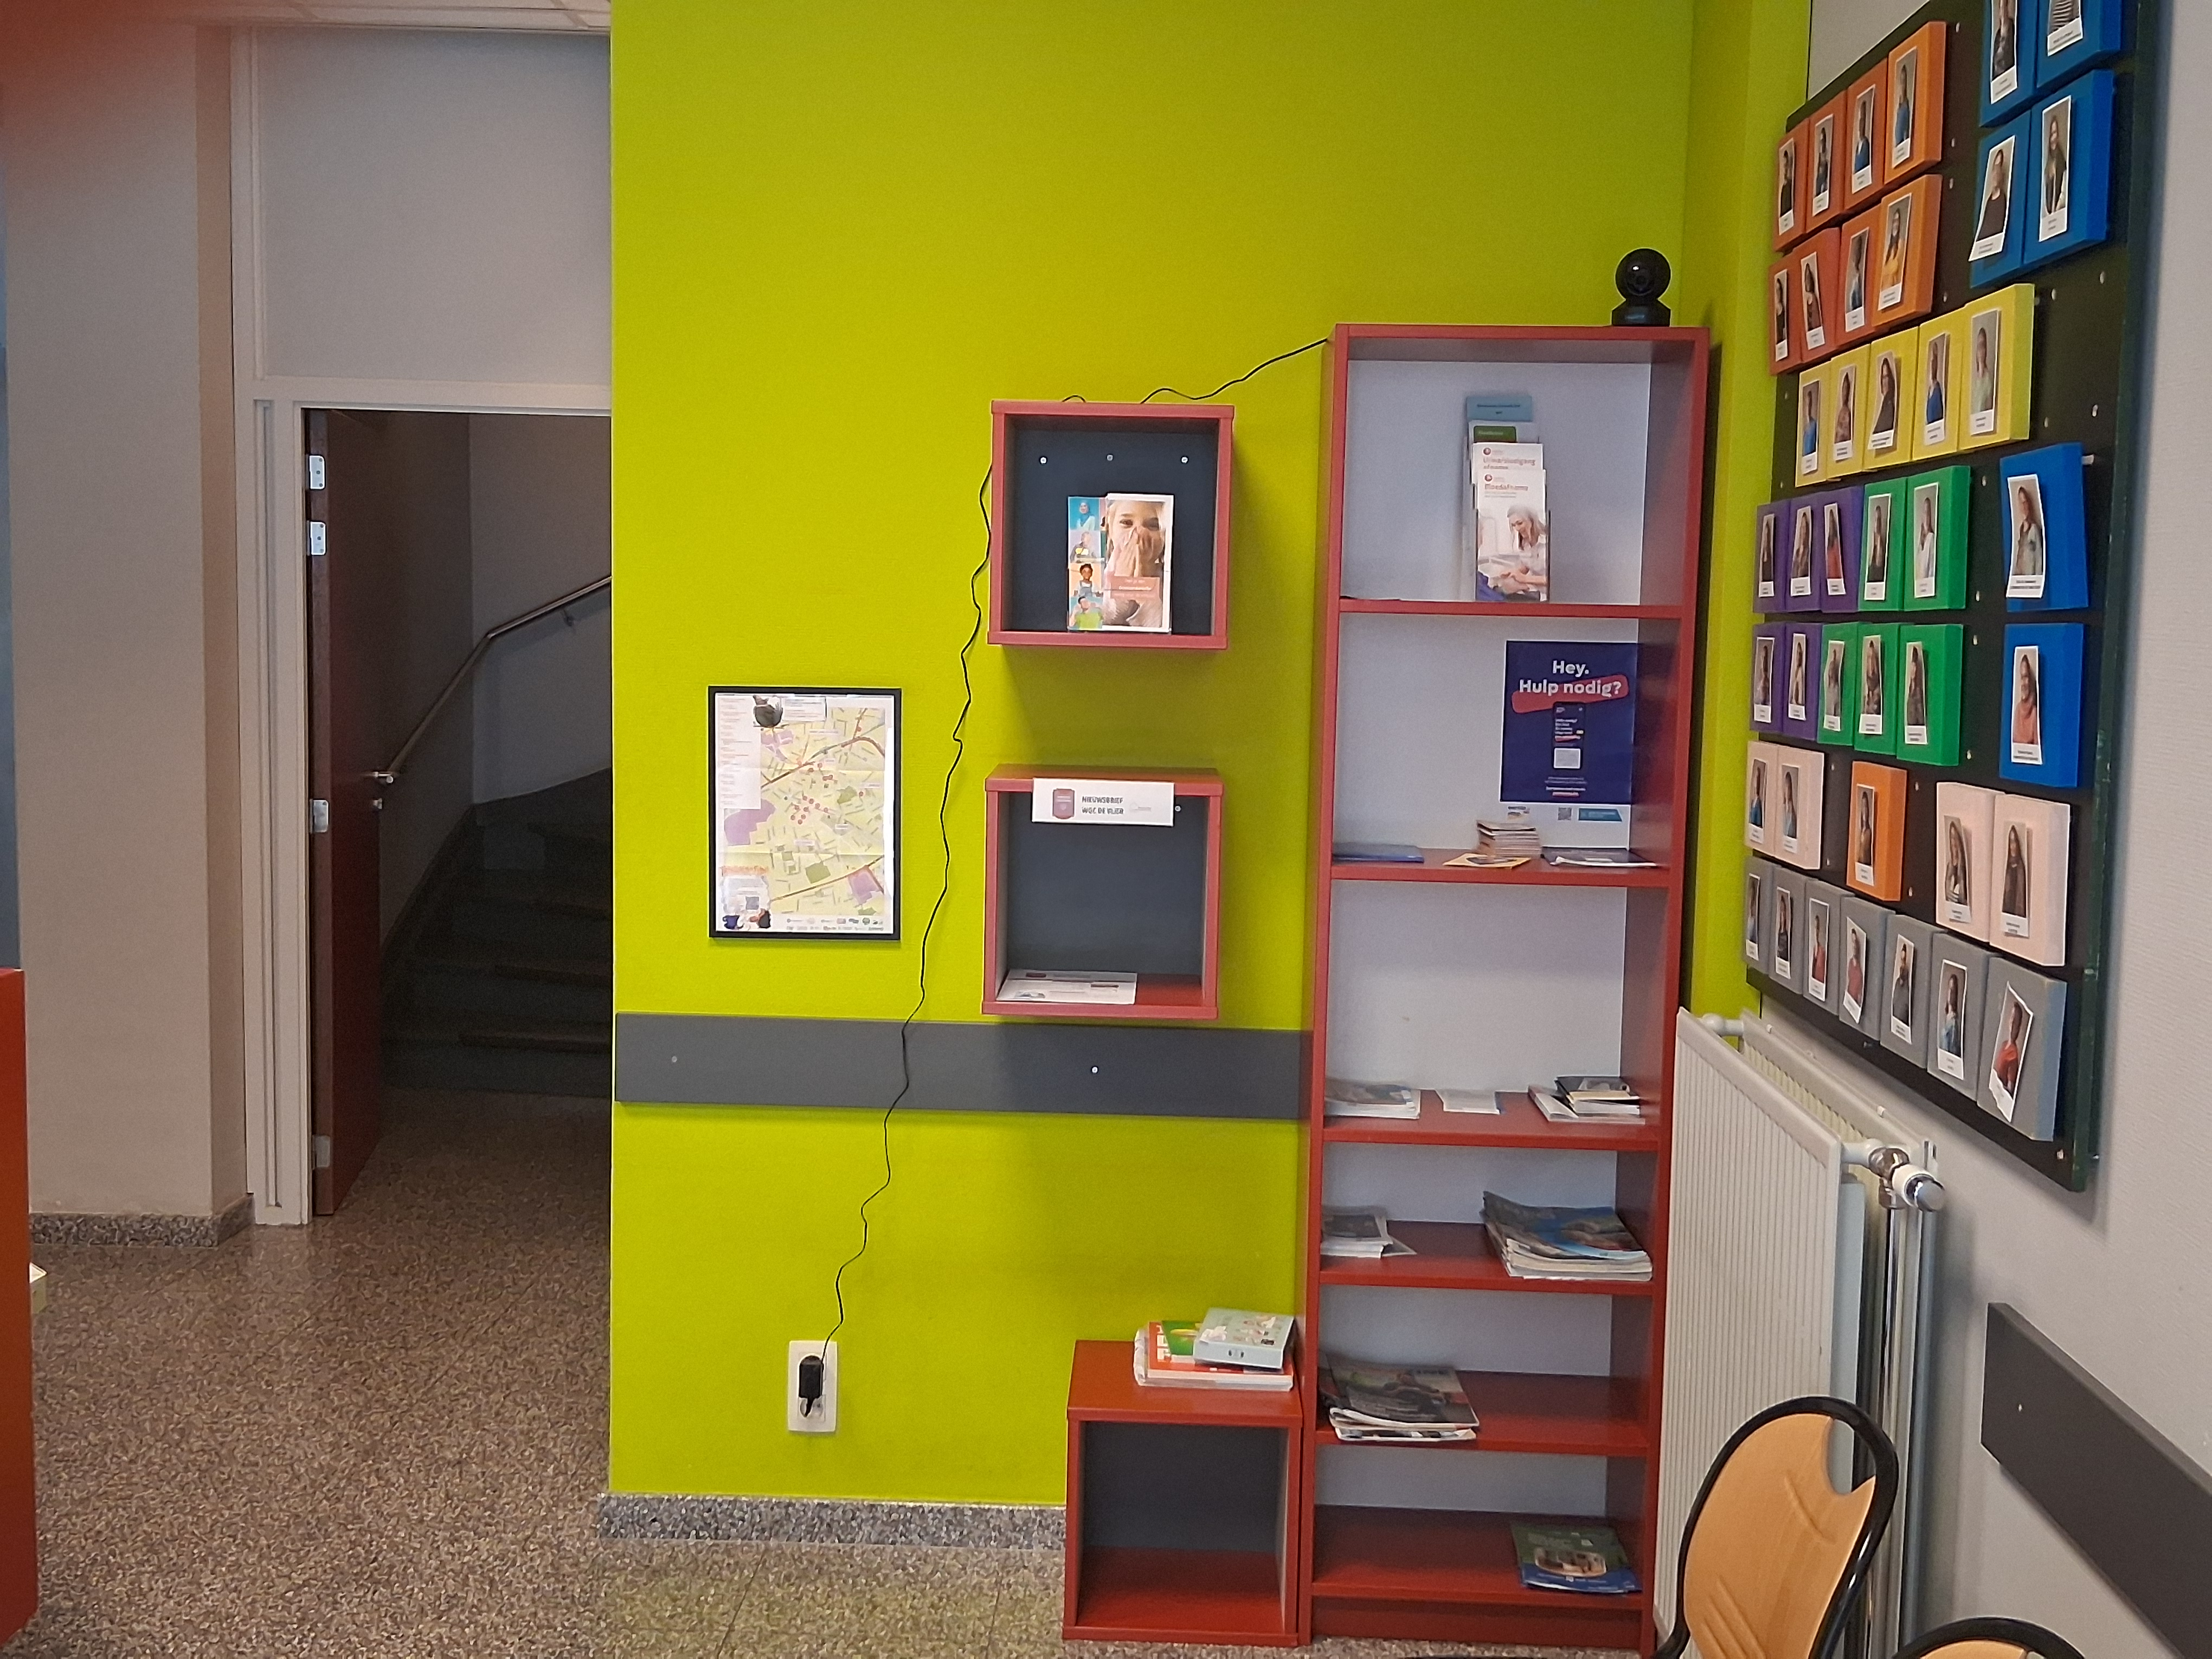
\includegraphics[width=\textwidth]{img/bp/vertex/camera-pic2.jpg}
    \end{minipage}
    \hfill
    \begin{minipage}[b]{0.49\textwidth}
        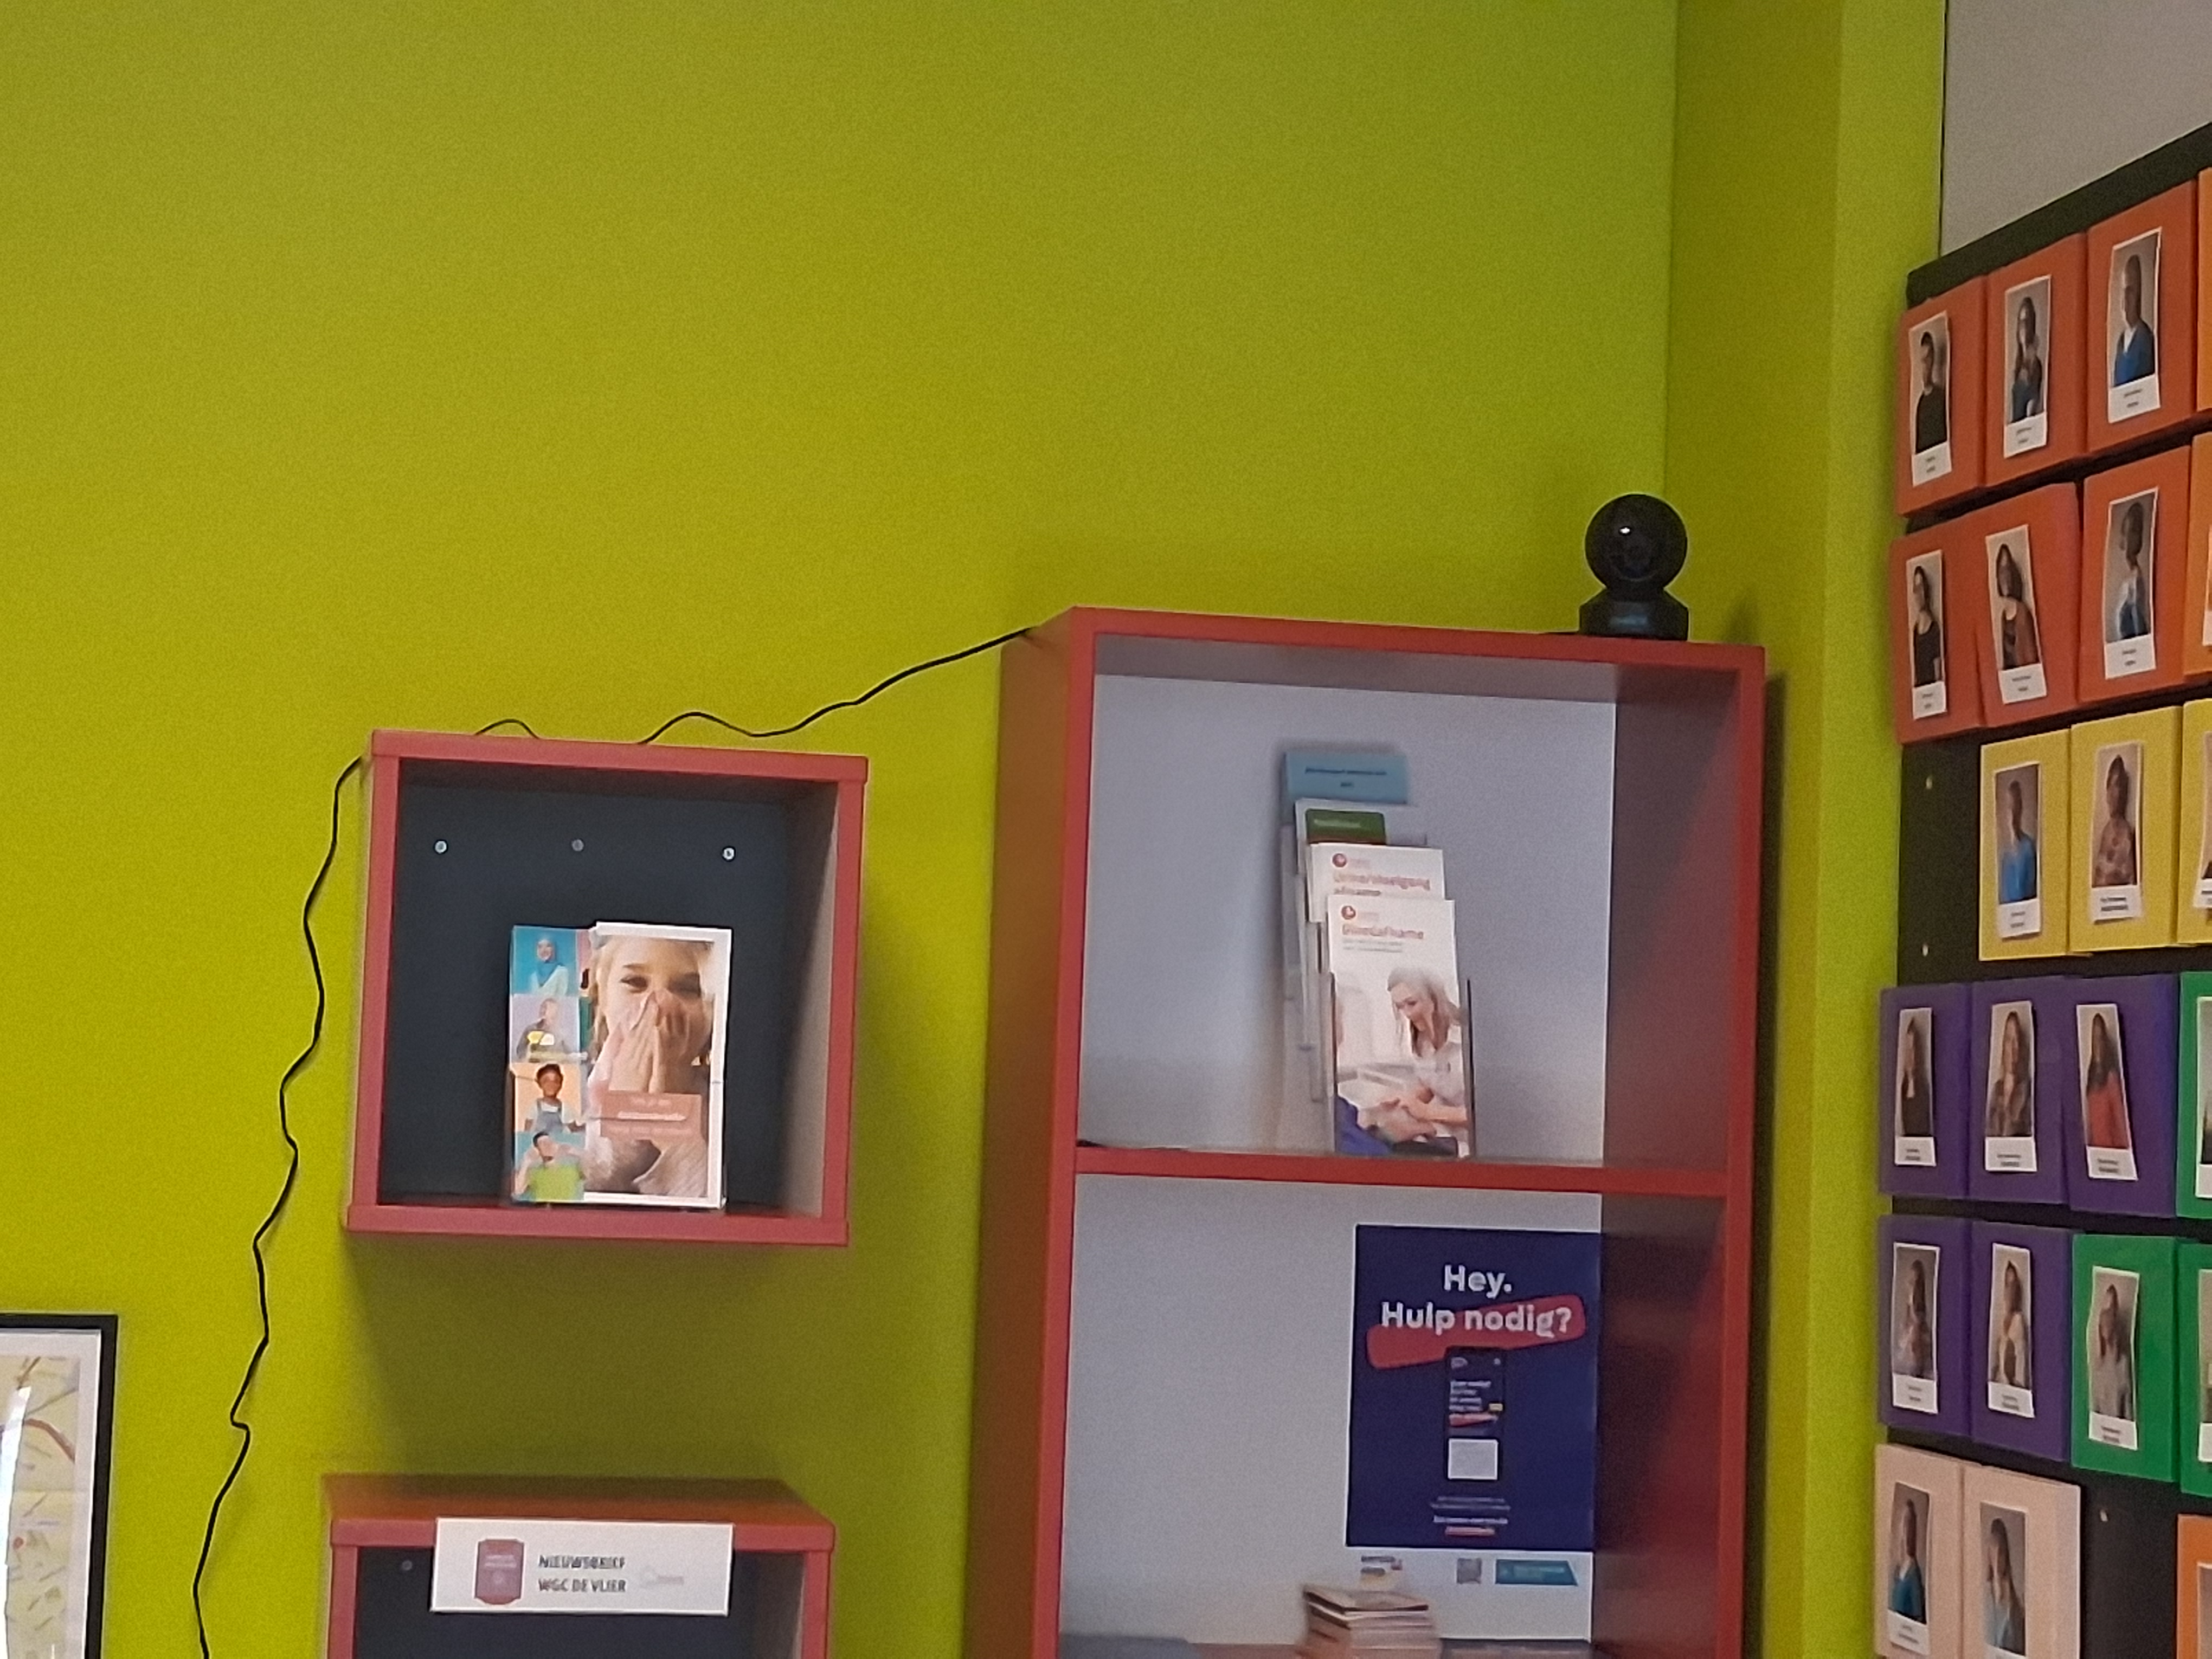
\includegraphics[width=\textwidth]{img/bp/vertex/camera-pic1.jpg}
    \end{minipage}
    
    \vspace{0.5em} % ruimte tussen rijen
    
    % Tweede rij met één afbeelding
    \begin{minipage}[b]{0.5\textwidth}
        \centering
        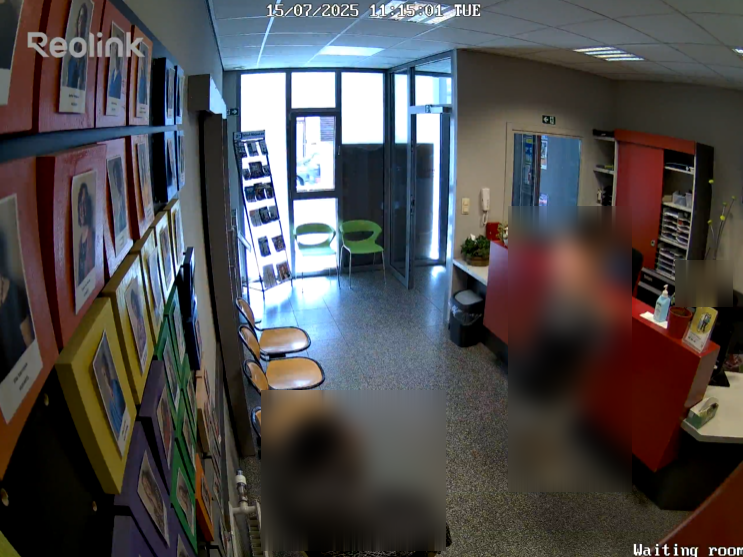
\includegraphics[width=\textwidth]{img/bp/vertex/camera_image_waitingroom_blurred.png}
    \end{minipage}
    
    \caption{Voorbeeldbeelden van de camera-interface (met blur zelf toegevoegd)}
    \label{fig:wgc-vertex-camera}
\end{figure}


\subsubsection{Integratie met Google Vertex AI Vision}
De configuratie van Vertex AI Occupancy Analytics werd uitgevoerd via de webconsole van Google Cloud Platform. \\

De officiële setupgids van Google \autocite{Cloud} werd gevolgd om:
\begin{itemize}
    \item Een BigQuery-dataset en -tabel aanmaken;
    \item Een Occupancy Analytics-app opzetten;
    \item De \gls{rtsp}-stream van de Reolink E1 Zoom koppelen;
    \item De output automatisch doorsturen naar BigQuery.
    \item Voorspellingen maken via ARIMA-PLUS
\end{itemize}

Door het volgen van de setupgids kon een consistente nulmeting uitgevoerd worden. De detectie werd vervolgens verfijnd met een eigen aanvulling.

\begin{figure}[H] 
    \centering
    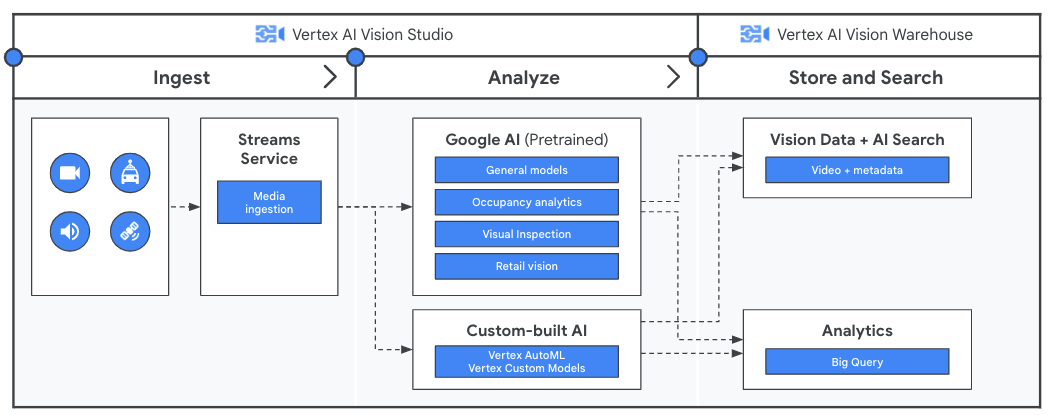
\includegraphics[width=\linewidth]{img/bp/vertex/vertex-flowchart.png}
    \caption{Overzicht van de gegevensstroom tijdens de nulmeting met Vertex AI \autocite{Cloud2025}}
    \label{fig:flowchart}
\end{figure}

\begin{figure}[H] 
    \centering
    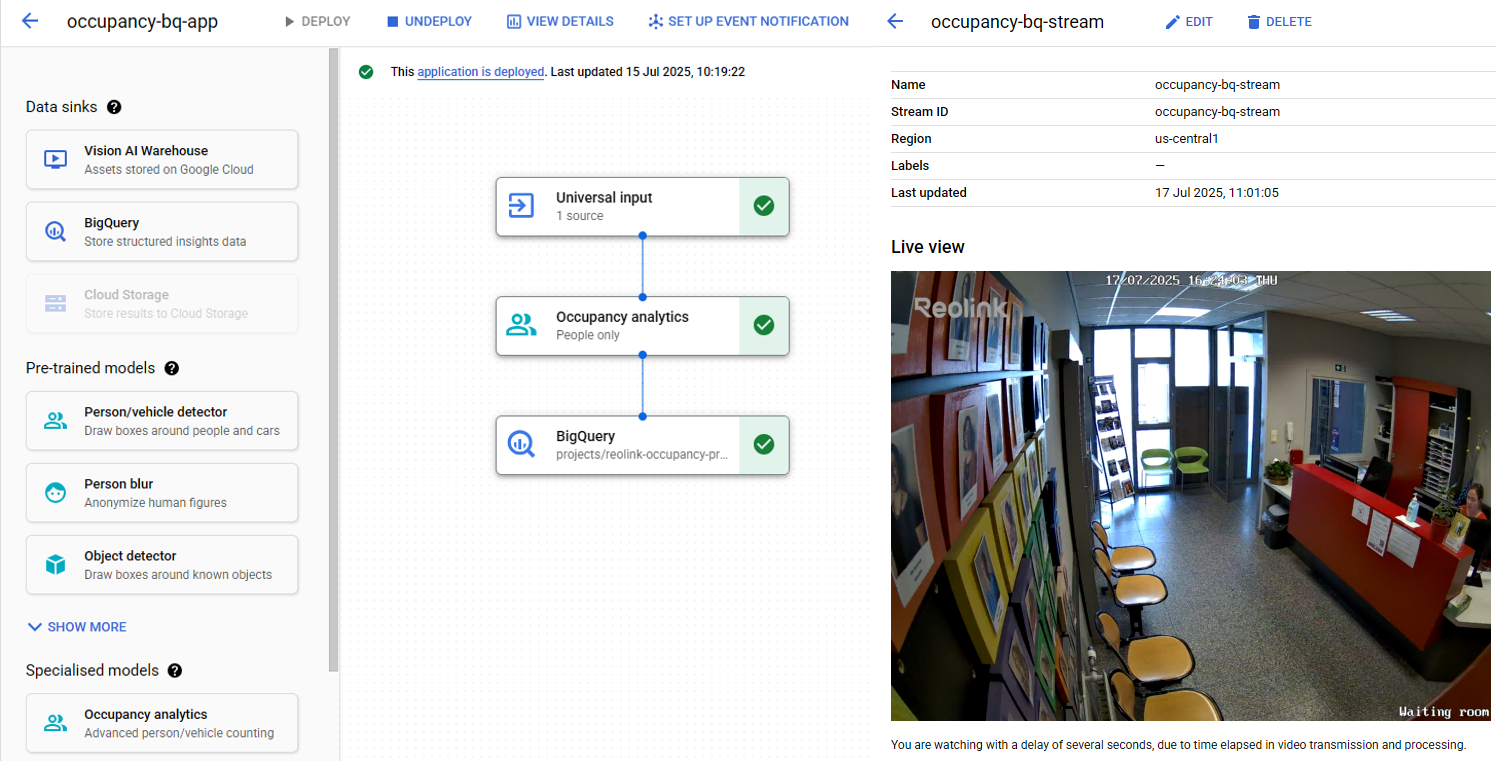
\includegraphics[width=16cm]{img/bp/vertex/combined_images.png}
    \caption{Configuratie en liveweergave van Google Vertex AI Occupancy Analytics}
    \label{fig:app}
\end{figure}

\subsubsection{Problemen en oplossingen tijdens configuratie}
Tijdens de testfase werd vastgesteld dat dezelfde persoon meerdere keren per seconde werd gedetecteerd. Dit leidde tot dubbeltellingen omdat er per frame geteld wordt. De trackId-parameter bleek niet bruikbaar door het feit dat deze constant op 0 stond. Er was bovendien een gebrek aan documentatie over het gebruik van trackId waardoor dit niet bruikbaar was. Om dit te compenseren, werd het volgende toegepast:
\begin{itemize}
    \item Een actieve zone afgebakend binnen de interface van Vertex AI;
    \item In de analyse werd per minuut enkel het maximale aantal personen behouden binnen de zone.
\end{itemize}    

Deze correcties verminderden de foutmarge en zorgden voor betrouwbaardere en reproduceerbare data.

\begin{figure}[H] 
    \centering
    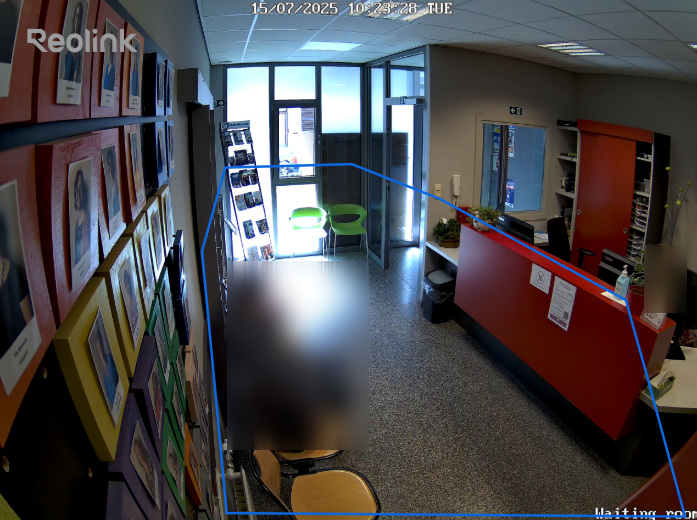
\includegraphics[width=10cm]{img/bp/vertex/active-zone (1).png}
    \caption{Afgebakende actieve zone in Google Vertex AI Occupancy Analytics (blauw kader)}
    \label{fig:active-zone}
\end{figure}
       

%\begin{figure}[h!]
    % Bovenste rij met drie foto's
   % \rotatebox{270}{%
%        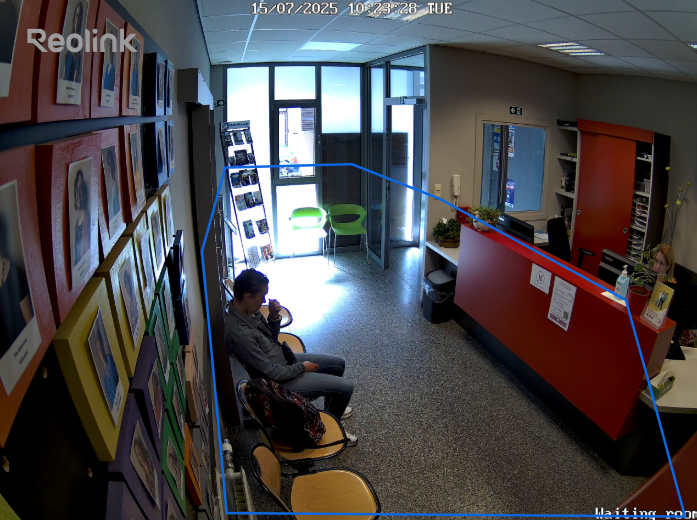
\includegraphics[width=0.5\textwidth]{img/bp/vertex/active-zone.png}
   % }
   % \hspace{0.01\textwidth}
    %\rotatebox{270}{%
      %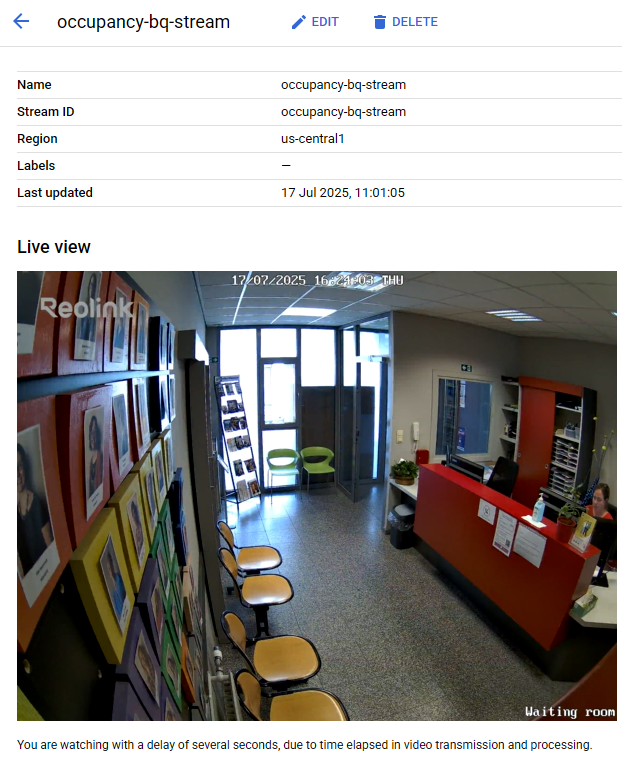
\includegraphics[width=0.5\textwidth]{img/bp/vertex/bq-stream.png}
   % }
   % \hspace{0.01\textwidth}
   % \rotatebox{270}{%
        %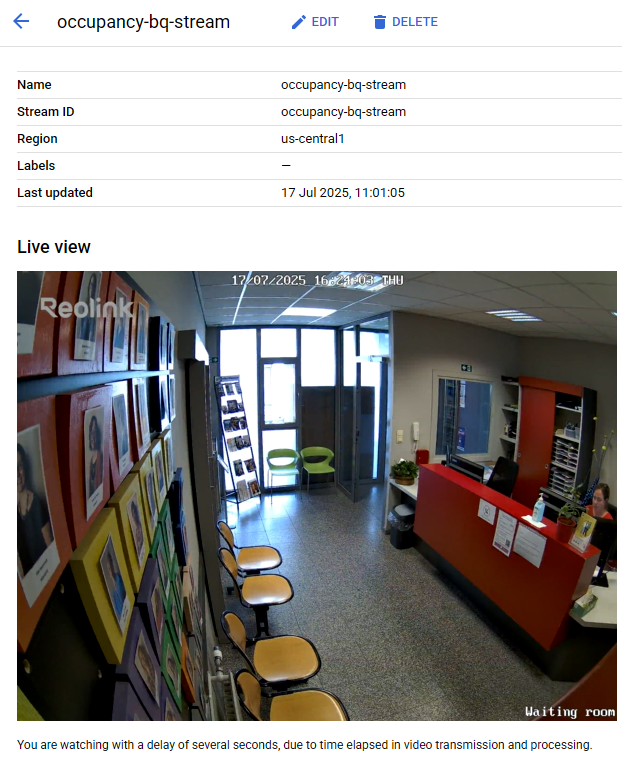
\includegraphics[width=0.8\textwidth]{img/bp/vertex/bq-stream.png}
    %}
    
    %\vspace{0.5em} % verticale ruimte tussen bovenste en onderste rij
    
    % Onderste foto
    %\rotatebox{0}{%
     %   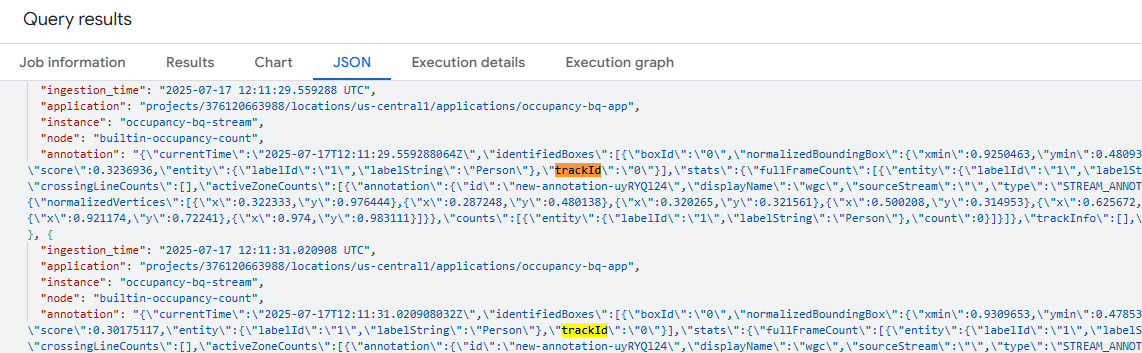
\includegraphics[width=1.2\textwidth]{img/bp/vertex/trackid.png}
    %}
    %\rotatebox{0}{%
    %    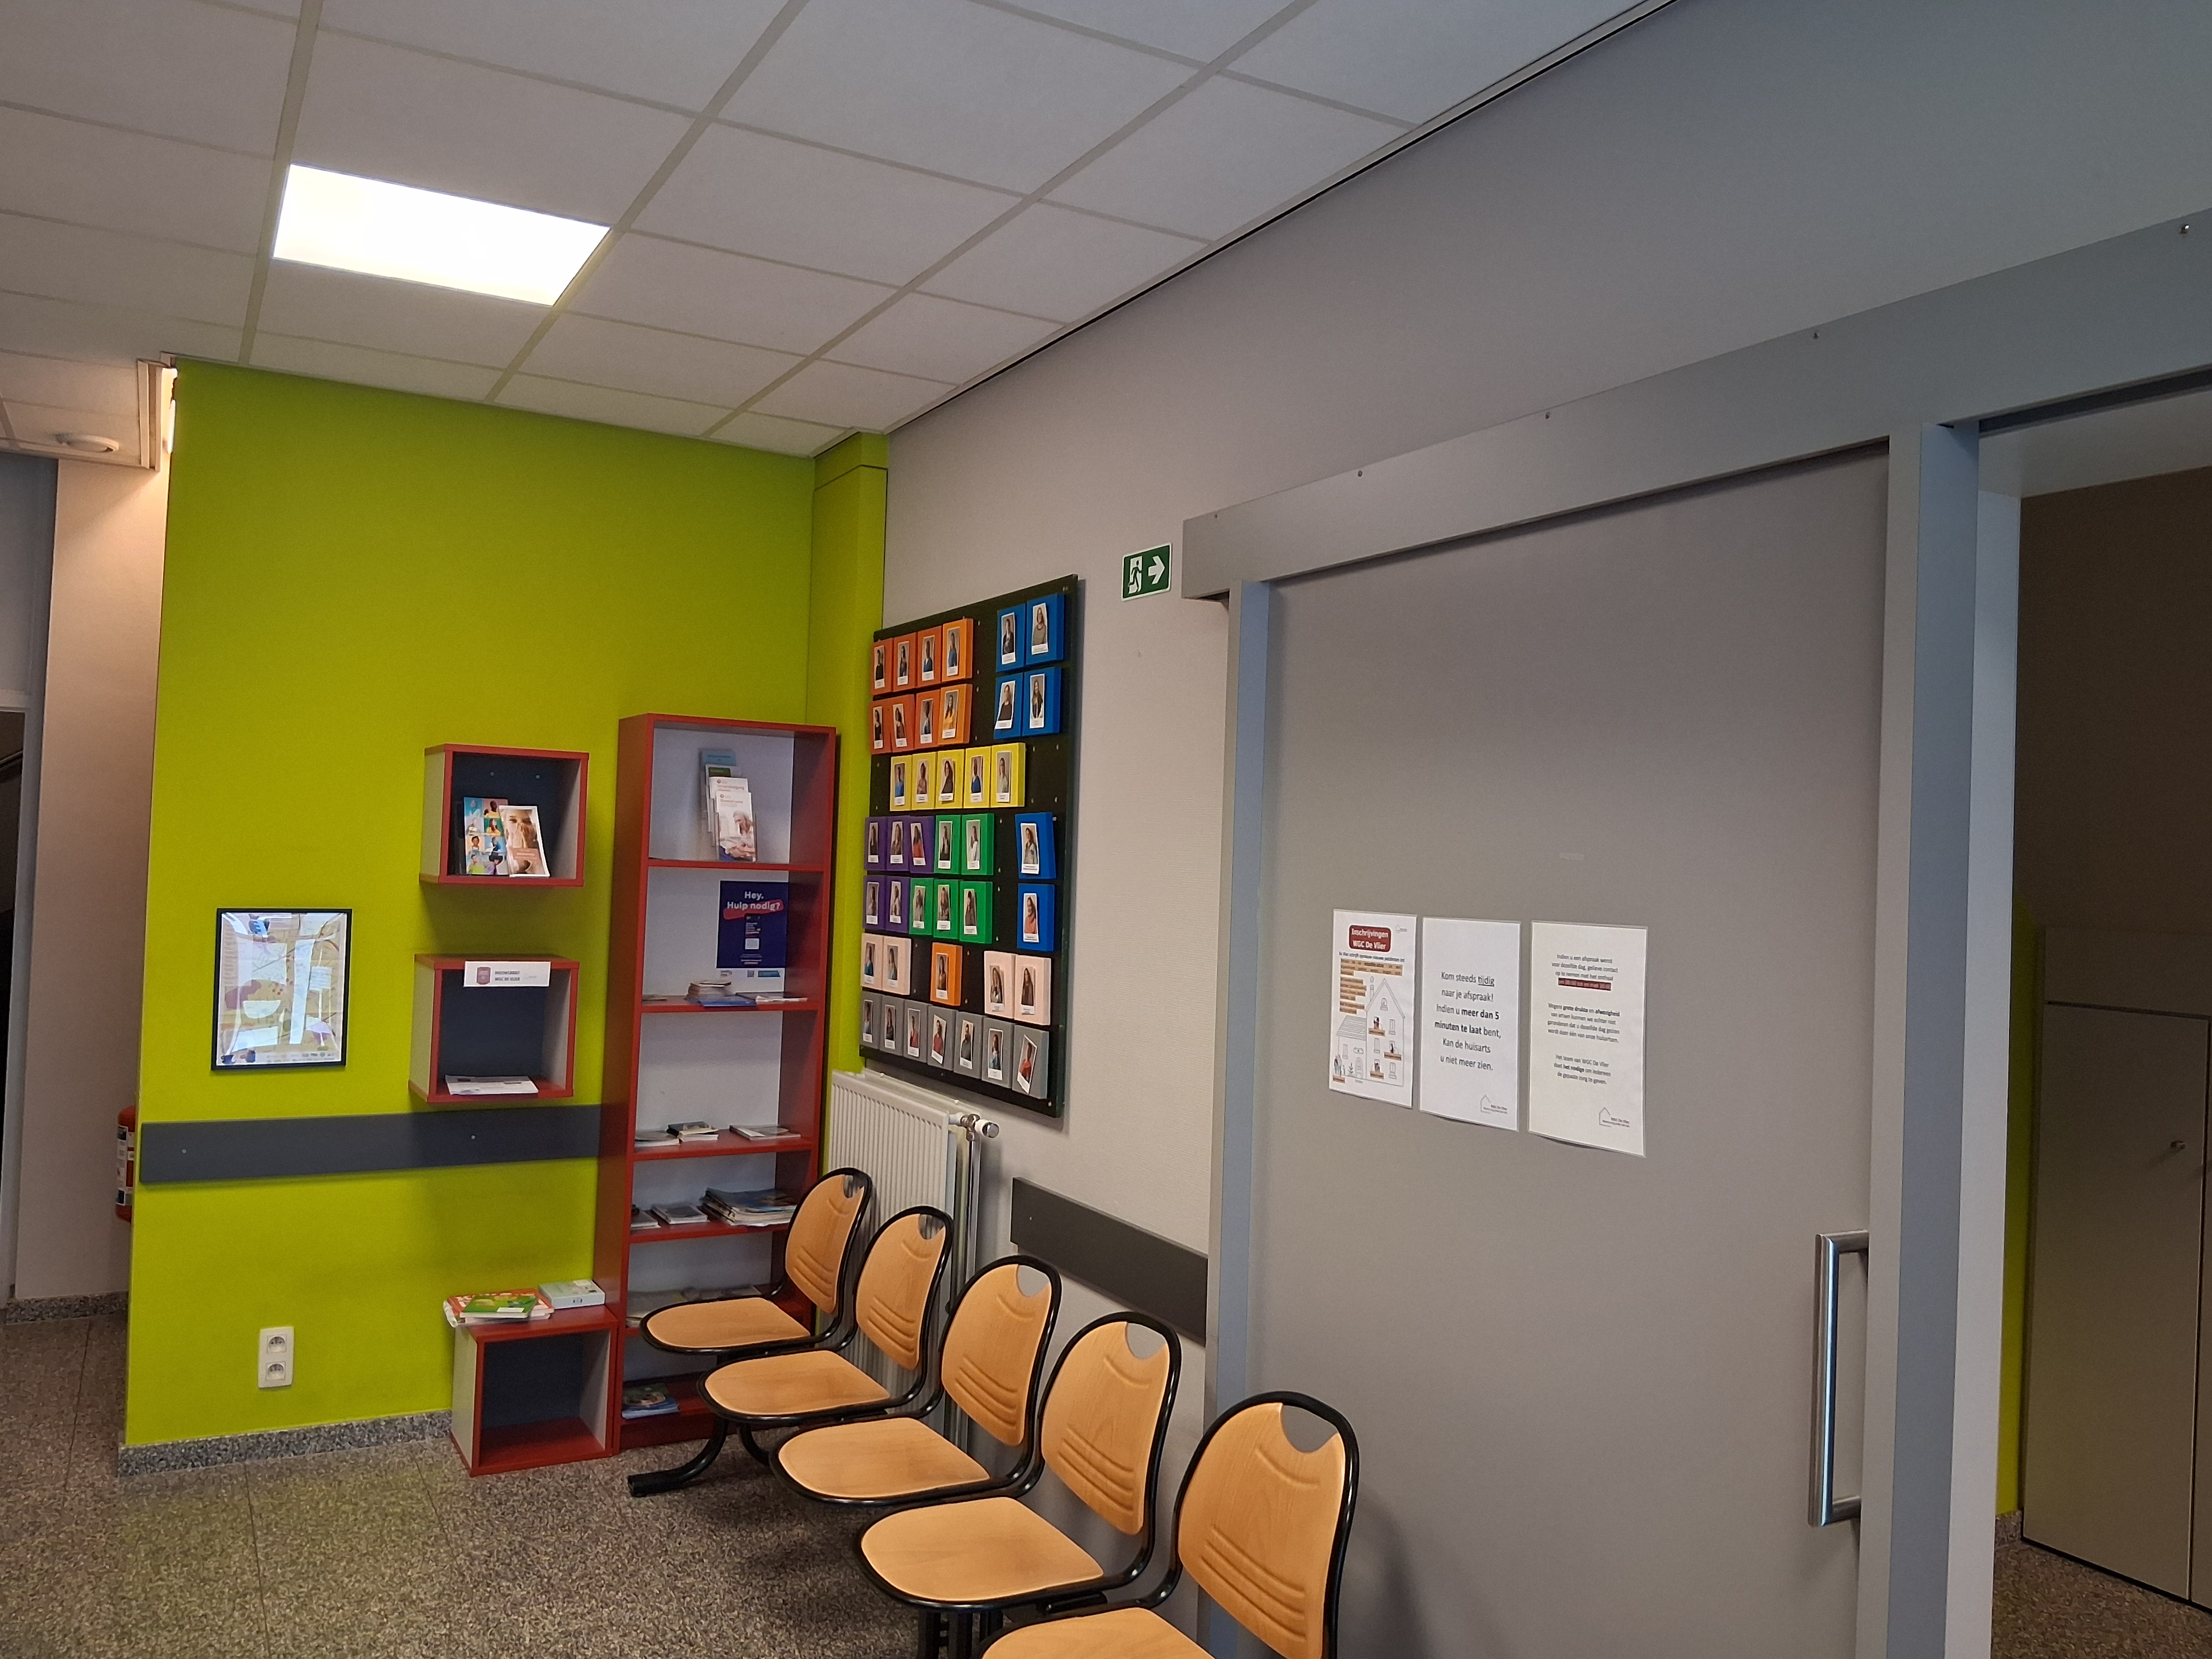
\includegraphics[width=0.46\textwidth]{img/bp/wachtruimtes/wachtruimte3.jpg}
    %}
    %\caption{Optioneel bijschrift}
 %   \label{fig:wgc-vertex}
%\end{figure}

\subsubsection{Verwerking van bezettingsdata via BigQuery}
De bezettingsdata gegenereerd door Vertex AI Vision werden automatisch opgeslagen in een Google BigQuery-dataset. Elke gedetecteerde persoon binnen de actieve zone (“wgc”) werd geregistreerd met een timestamp op minutenniveau.
Om fluctuaties binnen de data te verzachten werd er gekozen om het gemiddelde aantal personen per minuut te berekenen, dit zorgt voor een stabiele indicatie van de bezetting. Zie \ref{lst:tellingen} voor het codefragment.

\subsubsection{Validatie van de nulmeting}
Om de nauwkeurigheid van de metingen te controleren, werd op tien willekeurige tijdstippen manuele tellingen uitgevoerd tijdens één dag. Zie tabel \ref{tab:validatie_ai_manueel} \\

De manuele tellingen werden uitgevoerd door de camera feed te bekijken en het aantal aanwezige patiënten in de wachtruimte te noteren. \\   

De AI-metingen werden vergeleken met de manuele tellingen op basis van absolute verschillen. Deze methode werd als voldoende beschouwd voor de nulmeting omdat het doel van deze validatie is om na te gaan of de AI-metingen overeenkomen met de manuele tellingen. \\

Op basis van de vergelijking bedraagt het gemiddelde verschil ongeveer één tot twee personen, wat binnen dit onderzoek aanvaardbaar wordt beschouwd. Omdat de bezetting in de wachtruimte meestal laag is kunnen zelfs grote afwijkingen groot lijken. Daarom wordt de nulmeting vooral gebruikt als referentiepunt voor de evaluatie van het \gls{iot}-systeem en de voorspellende modellen. 

\begin{table}[H]
    \caption{Vergelijking tussen AI-meting en manuele telling tijdens de nulmeting van 16-07}
    \label{tab:validatie_ai_manueel}
    \centering
    \begin{tabular}{@{}lcccc@{}}
        \toprule
        \textbf{Tijdstip} & \textbf{Gemiddelde detectie (AI)} & \textbf{Afgerond (AI-meting)} & \textbf{Manueel} & \textbf{Verschil} \\
        \midrule
        08:15 & 2.706 & 3 & 2 & +1 \\
        09:45 & 1.255 & 1 & 2 & -1 \\
        10:15 & 2.378 & 2 & 4 & -2 \\
        11:00 & 1.000 & 1 & 1 & 0 \\
        12:15 & 6.292 & 6 & 3 & +3 \\
        14:30 & 1.878 & 2 & 2 & 0 \\
        15:15 & 1.925 & 2 & 3 & -1 \\
        16:45 & 0.903 & 1 & 1 & 0 \\
        17:30 & 0.000 & 0 & 0 & 0 \\
        18:15 & 0.000 & 0 & 0 & 0 \\
        \bottomrule
    \end{tabular}
\end{table}

\subsubsection{Voorspellende analyse met ARIMA-PLUS}
ARIMA\_PLUS werd gekozen voor het voorspellen van de bezettingsgraad binnen de wachtruimte van \gls{wgc} De Vlier. Dit model werd gekozen door de eenvoud van implementatie, de geschiktheid voor univariate tijdreeksen, en dat dit model direct geïntegreerd is in BigQuery. Door deze keuze kon het model rechtstreeks uitgevoerd worden op de data zonder het gebruik van externe tools of complexe machine learning frameworks.  \\

Voor de training van het ARIMA\_PLUS-model in BigQuery werd gekozen om \texttt{avg\_people} (Gemiddelde detectie (AI)) te gebruiken, zodat het model de nauwkeurigheid en fluctuaties in de data houdt. ARIMA\_PLUS is een tijdreeksmodel zonder ondergrens, waardoor voorspellingen soms negatief kunnen zijn. Omdat negatieve aantallen niet realistisch zijn, worden deze voorspellingen op nul gezet: 

\begin{verbatim}
    GREATEST(forecast_value, 0) AS predicted_avg_people
\end{verbatim}

Daarnaast toont het ARIMA\_PLUS-model ook enkele negatieve voorspellingen (zie Tabel~\ref{tab:voorspellingen_a}), die in de context van een bezettingsgraad geen betekenis hebben. Deze artefacten vergroten de foutscore en benadrukken de beperkingen van het model.

\begin{table}[H]
    \small
    \begin{tabular}{|p{3.5cm}|p{2.5cm}|p{3cm}|p{4.8cm}|}
        \hline
        \textbf{Datum \& Tijd (UTC)} & \textbf{Voorspelling} & \textbf{Standaardfout} & \textbf{Betrouwbaarheidsniveau} \\
        \hline
        2025-07-22 09:41:00 & 0.285961 & 0.209584 & 0.95 \\
        2025-07-22 16:58:00 & 0.239966 & 0.405759 & 0.95 \\
        2025-07-22 16:01:00 & 0.245965 & 0.385149 & 0.95 \\
        2025-07-22 07:58:00 & 0.296802 & 0.130000 & 0.95 \\
        2025-07-22 17:21:00 & 0.237545 & 0.413842 & 0.95 \\
        2025-07-22 22:57:00 & 0.202180 & 0.520711 & 0.95 \\
        2025-07-23 06:03:00 & 0.157342 & 0.637255 & 0.95 \\
        2025-07-23 06:35:00 & 0.153974 & 0.645451 & 0.95 \\
        2025-07-23 02:52:00 & 0.177446 & 0.586886 & 0.95 \\
        2025-07-22 10:57:00 & 0.277962 & 0.253408 & 0.95 \\
        \hline
    \end{tabular}
    \caption{ARIMA\_PLUS voorspellingen met standaardfout en betrouwbaarheidsniveau.}
    \label{tab:voorspellingen_a}
\end{table}

\begin{table}[H]
    \small
    \begin{tabular}{|p{3.5cm}|p{3cm}|p{3cm}|p{3cm}|p{3cm}|}
        \hline
        \textbf{Datum \& Tijd (UTC)} & \textbf{Ondergrens (PI)} & \textbf{Bovengrens (PI)} & \textbf{Ondergrens (CI)} & \textbf{Bovengrens (CI)} \\
        \hline
        2025-07-22 09:41:00 & -0.124081 & 0.696004 & -0.124081 & 0.696004 \\
        2025-07-22 16:58:00 & -0.553885 & 1.033817 & -0.553885 & 1.033817 \\
        2025-07-22 16:01:00 & -0.507562 & 0.999492 & -0.507562 & 0.999492 \\
        2025-07-22 07:58:00 & 0.042463  & 0.551142 & 0.042463  & 0.551142 \\
        2025-07-22 17:21:00 & -0.572120 & 1.047210 & -0.572120 & 1.047210 \\
        2025-07-22 22:57:00 & -0.816569 & 1.220929 & -0.816569 & 1.220929 \\
        2025-07-23 06:03:00 & -1.089421 & 1.404105 & -1.089421 & 1.404105 \\
        2025-07-23 06:35:00 & -1.108825 & 1.416773 & -1.108825 & 1.416773 \\
        2025-07-23 02:52:00 & -0.970772 & 1.325663 & -0.970772 & 1.325663 \\
        2025-07-22 10:57:00 & -0.217820 & 0.773744 & -0.217820 & 0.773744 \\
        \hline
    \end{tabular}
    \caption{ARIMA\_PLUS voorspellingen met onder- en bovengrenzen (PI en CI).}
    \label{tab:voorspellingen_b}
\end{table}



Zie Lijstingen \ref{lst:people_forecast_model} en \ref{lst:people_forecast_query} voor de codefragmenten.

\subsubsection{Gebruik van MAPE voor het evalueren van ARIMA-PLUS}
Om het ARIMA\_PLUS model te evalueren werd er gekozen om de Mean Absolute Percentage Error (MAPE) te berekenen. MAPE wordt gebruikt om de nauwkeurigheid van een voorspellend model te beoordelen. Het drukt de gemiddelde fout uit in procenten en geeft de gemiddelde afwijking in procenten wat de interpretatie eenvoudig en transparant maakt. MAPE wordt ook breed toegepast in tijdreeksvoorspellingen.

\subsubsection{Evaluatie van de nauwkeurigheid van het voorspellingsmodel (t.o.v. \gls{wgc}-observaties)}
MAPE wordt berekend tussen de voorspelde waarden en de \gls{wgc}-observaties. Voor de berekening wordt de volgende formule toegepast: 

\[
\mathrm{MAPE} = \frac{100\%}{n} \sum_{i=1}^n \left| \frac{\hat{y}_i - y_i}{y_i} \right|
\]

$\hat{y}_i$ in deze formule is de voorspelde waarde en $y_i$ de geobserveerde waarde. Tijdstippen met $y_i = 0$ zijn niet inbegrepen om deling door nul te vermijden. \\

De MAPE bedraagt \textbf{67,81\%}, berekend over \textbf{84 overlappende minuten}. Dit betekent dat de voorspellingen gemiddeld meer dan twee derde afwijken van de gemeten waarden. Maar dit moet wel genuanceerd worden: bij lage bezettingsgraden leiden zelfs kleine absolute verschillen al snel tot hoge procentuele fouten. Het codefragment voor het berekenen van de MAPE: \ref{lst:people_forecast_mape} 



%Door lineaire interpolatie van de uurbasis-forecast naar minuutniveau kon de voorspelling beter worden afgestemd op de gemeten \gls{iot}-data. Ondanks deze verfijning blijft de fout relatief groot, wat erop wijst dat het model de korte-termijnfluctuaties in de bezetting niet volledig kan opvangen.


\subsubsection{Interpretatie van de resultaten} 
De ARIMA\_PLUS-voorspellingen toonden aan dat de geschatte bezettingsgraad vaak laag ligt, met waarden die in sommige gevallen negatief uitkomen. Deze negatieve voorspellingen zijn artefacten van het model en worden in de praktijk op nul gezet, wat de foutmarges beïnvloedt. De betrouwbaarheidsintervallen zijn relatief breed, vooral bij tijdstippen met weinig mensen, wat aangeeft dat het model onzekerheid heeft bij lage bezettingsniveau. \\

De berekende MAPE van 67,81\% bevestigt dat de voorspellingen aanzienlijk kunnen afwijken van de werkelijke observaties. Dit betekent niet dat het model volledig onbruikbaar is, maar vooral dat het moeite heeft om nauwkeurig te voorspellen bij lage bezettingsniveaus, waar zelfs kleine absolute verschillen procentueel zwaar wegen. Kortom, ARIMA\_PLUS kan trends in de bezetting aangeven, maar de absolute voorspellingen moeten met voorzichtigheid geïnterpreteerd worden, vooral bij lage bezoekersaantallen.


%Voor de volledige dataset wordt verwezen naar Bijlage~\ref{bijlage:wgc-data.csv}.


%\subsubsection{Nulmeting als benchmark voor \gls{iot}-validatie}
%De resultaten uit de nulmeting vormen een belangrijk referentiepunt voor de beoordeling van de nauwkeurigheid en betrouwbaarheid van het \gls{iot}-systeem. In het volgende onderdeel wordt dit systeem opgebouwd en gevalideerd aan de hand van deze referentiegegevens.


%\subsubsection{Meervoudige telling voorkomen}
%Occupancy Analytics is een model binnen Vertex AI is gericht op het detecteren en tellen van mensen. In de context van dubbeltellingen werd in deze model een extra intelligentie ingebouwd om te voorkomen dat dezelfde persoon meerdere keren geteld wordt wat cruciaal is voor nauwkeurige analyse, toch werd ervoor gekozen om per minuut het maximum aantal personen te behouden, in plaats van het aantal gedetecteerde frames. Zo werd voor de zekerheid vermeden dat dezelfde persoon meerdere keren per seconde zou worden meegeteld. 



\subsection{Opbouw van het \gls{iot}-meetsysteem}
Het \gls{iot}-systeem maakt gebruik van een ESP32 (sensorcontroller) en een Raspberry Pi (centrale eenheid) voor lokale opslag. De sensoren binnen dit systeem tellen het aantal personen bij doorgangen wat ideaal is voor een kleine wachtruimte. Het \gls{iot}-systeem werd als volgt opgebouwd: 

\begin{itemize}
    \item Twee Adafruit \gls{ir} Break Beam-sensoren aan weerszijden van de deur/doorgang (in/uitrichting) geplaatst met niet-permanente bevestiging.
    \item ESP32 leest GPIO-onderbrekingen, verwerkt lokaal en stuurt data via Wi-Fi naar InfluxDB (Raspberry Pi).
    \item Raspberry Pi slaat de data op in InfluxDB
    \item Privacyvriendelijke opzet: enkel telwaarden worden behandeld.
\end{itemize}

%In het Proof of Concept (\gls{poc}) wordt een eenvoudige \gls{iot}-architectuur gebruikt waarbij sensoren in real-time registreren hoeveel mensen aanwezig zijn. De metingen gebeuren volledig anoniem. De verzamelde gegevens worden automatisch doorgestuurd naar een timeseries-database voor opslag. \\

%Het meetsysteem maakt gebruik van twee Adafruit \gls{ir} Break Beam-sensoren, die aan weerszijden van de toegangsdeur tot de wachtruimte zijn geplaatst met niet-permanente bevestiging, zodat ze eenvoudig verwijderbaar zijn zonder schade aan de infrastructuur. De ene sensor registreert binnenkomende bewegingen, de andere uitgaande. Door het verschil tussen beide tellers wordt het actuele aantal aanwezige personen berekend. \\

%De sensoren zijn verbonden met een ESP32-WROOM microcontroller. Deze leest de onderbrekingen via digitale GPIO-pinnen en verwerkt de gegevens lokaal. De ESP32 verstuurt de data via Wifi in real-time door naar een InfluxDB-database, die op een Raspberry Pi draait in het lokale netwerk. Deze opstelling vermijdt externe cloudafhankelijkheid en garandeert de privacy van de bezoekers, omdat enkel telwaarden worden opgeslagen. \\

%Deze opstelling maakt het mogelijk om op eenvoudige en privacyvriendelijke wijze real-time het aantal aanwezigen in de wachtruimte te meten. Aangezien er geen beelden worden opgeslagen en enkel telgegevens worden verstuurd, blijft de impact op de privacy minimaal. \\


%\begin{figure}[H] 
%    \centering
%    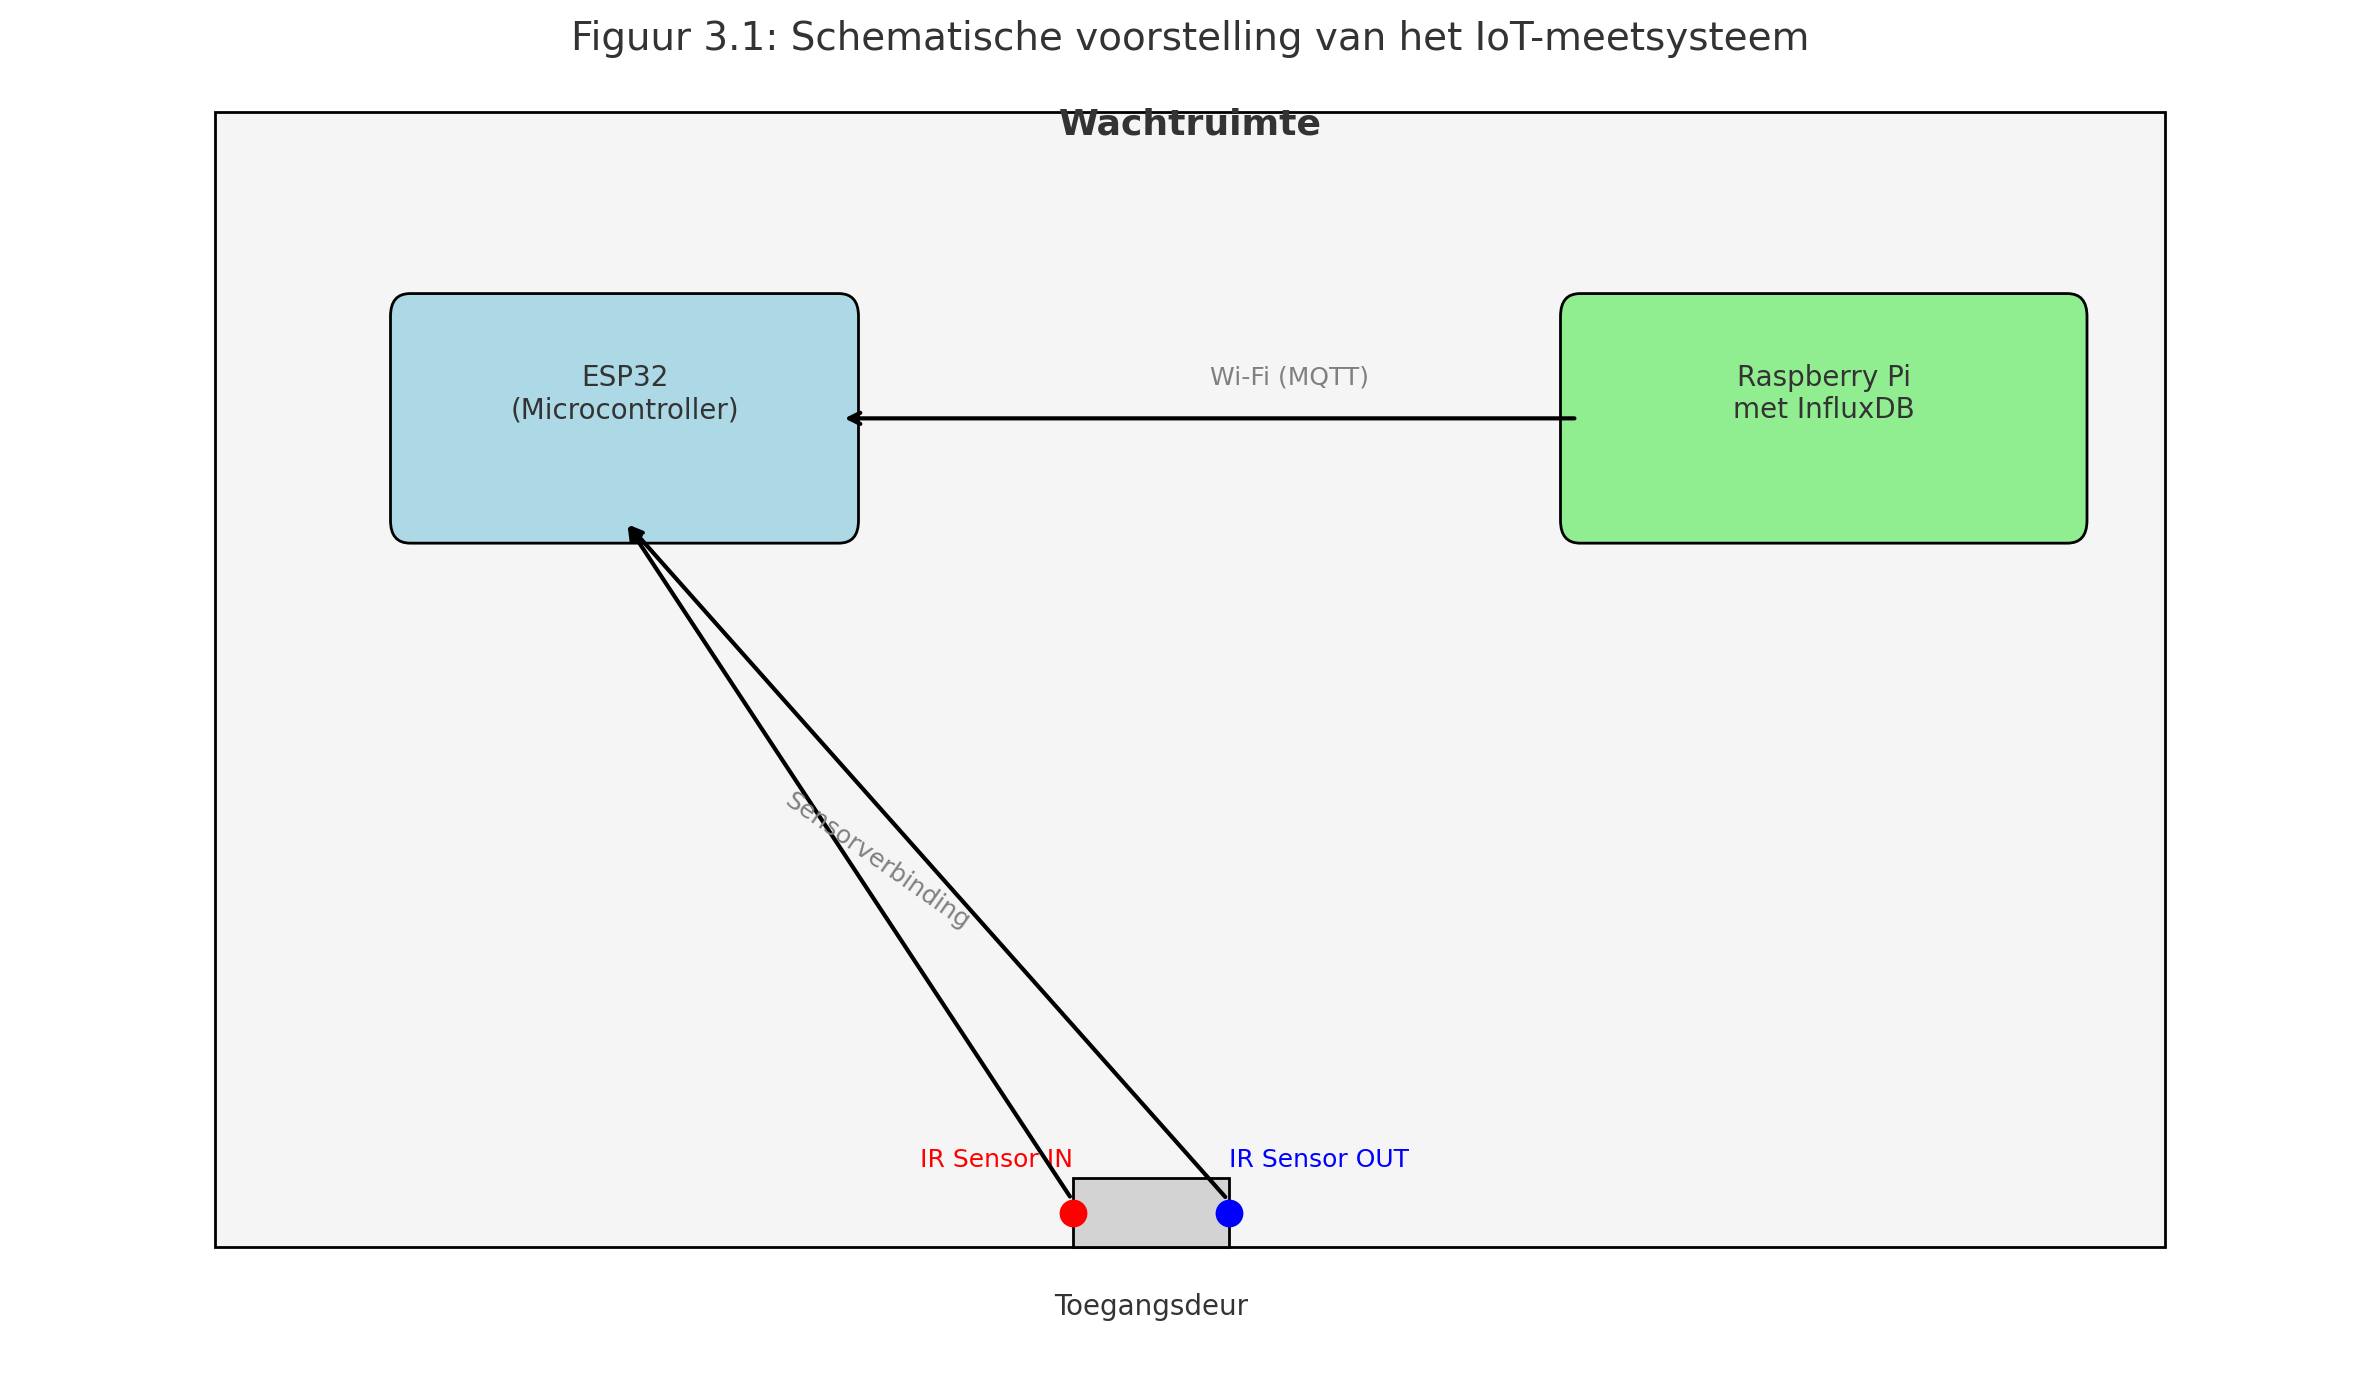
\includegraphics[width=\linewidth]{img/bp/iot-schema.png}
%    \caption{Schematische voorstelling van het \gls{iot}-meetsysteem met \gls{ir}-sensoren en lokale dataverwerking via InfluxDB}
%    \label{fig:iot-flowchart}
%\end{figure}


\subsubsection{Motivering sensorkeuze}
Bij het ontwerpen van het meetsysteem werd gekeken naar de mogelijkheid om ultrasone (HC-SR04) en/of passieve infrarood (HC-SR501) sensoren te combineren met de twee Adafruit \gls{ir} Break Beam-sensoren. \\

Uiteindelijk werd ervoor gekozen om enkel de break beam-sensoren te gebruiken, deze keuze werd gemaakt door de kleine wachtruimte en het grote aantal bekabeling van de break beam-sensoren. Verder maakt de aanwezigheid van kinderen het moeilijk om het systeem veilig en ongestoord te laten werken. Om deze reden is het gebruik van extra sensoren minder praktisch en betrouwbaar. \\

\subsection{Technische uitwerking}
Het \gls{poc}-meetsysteem gebruikt de infrarood break beam-sensoren om bewegingen in de wachtruimte te registreren. De sensoren werden aan beide zijden van de doorgang geplaatst om te bepalen of iemand binnenkomt of vertrekt, en in welke richting, wat dubbele of foutieve detecties voorkomt.\\

Het systeem werkt volledig anoniem en real-time zonder gebruik van camera’s of andere persoonsherkenningstechnieken. De volgende secties behandelen hardware, logica en dataverwerking in detail.

\subsubsection{Hardwarecomponenten}
\begin{itemize}
    \textbf{ESP32-WROOM}: Wordt ingezet voor het uitlezen van de \gls{ir}-sensoren en het versturen van bezettingsdata naar InfluxDB via Wi-Fi.   
    \item \textbf{\gls{ir} break beam sensoren (2x)}: Bestaan elk uit een infraroodzender en -ontvanger.
\end{itemize}

\begin{figure}[htbp]
    \centering
    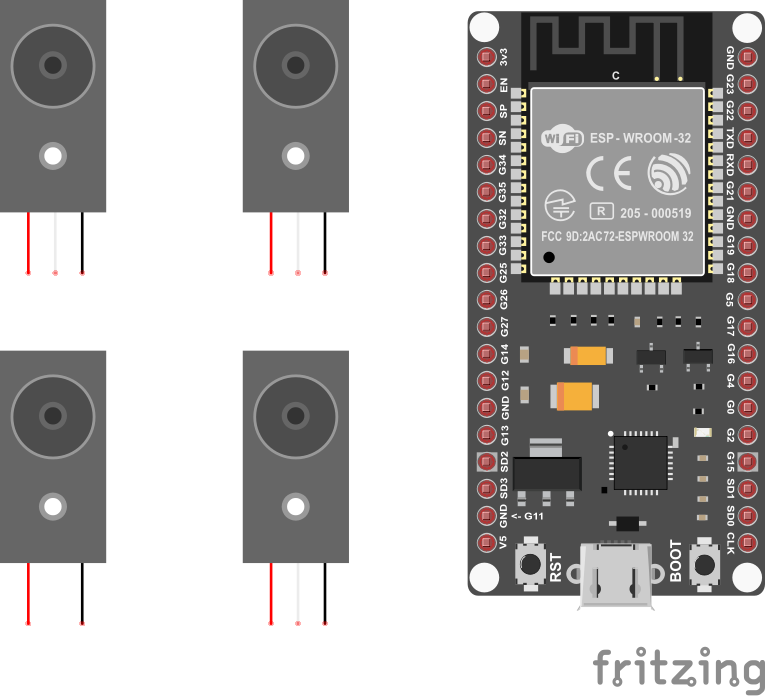
\includegraphics[width=8cm]{img/bp/wachtruimtes/technische_uitwerking/componenten.png}
    %\caption{Breadboardopstelling met ESP32 en Adafruit \gls{ir} Break Beam sensoren (gemaakt in Fritzing)}
    \label{fig:componenten}
\end{figure}

\subsubsection{Positionering van de sensoren in de meetomgeving}
De \gls{ir} break beam-sensoren werden tegenover elkaar geplaatst in de deuropening, op ongeveer halve deurhoogte. Het is essentieel dat zowel de emitter en receiver precies tegenover elkaar gepositioneerd zijn. De bovenste sensor werd iets dieper in de doorgang geplaatst dan de onderste. Zo wordt bij binnenkomst eerst de bovenste sensor onderbroken, en bij het verlaten van de ruimte eerst de onderste. Dit laat toe om via volgorde van onderbrekingen de looprichting correct te bepalen. %De sensoren zijn bevestigd met elektrische tape, op een locatie zonder ramen of reflecterende oppervlakken om meetfouten te vermijden.

\subsubsection{Detectielogica en tellingsmethode}
De ESP32 registreerde de onderbrekingen van de infraroodstralen via de digitale inputpinnen. Door de volgorde van de onderbrekingen te analyseren kan worden afgeleid of iemand \textit{binnenkwam} of \textit{buitenging}.

\begin{itemize}
    \item Volgorde \texttt{Sensor In} gevolgd door \texttt{Sensor Out} binnen een tijdsinterval van 3 seconden $\Rightarrow$ \textbf{toename} (\texttt{+1}) van het aantal aanwezigen (\texttt{peopleCount}).
    \item Volgorde \texttt{Sensor Out} gevolgd door \texttt{Sensor In} binnen 3 seconden $\Rightarrow$ \textbf{afname} (\texttt{-1}) van het aantal aanwezigen (\texttt{peopleCount}).
\end{itemize}

\textbf{Debouncing} werd toegepast om storingen en dubbele detecties te voorkomen, hierbij werd een minimale stabilisatietijd van 30 milliseconden tussen opeenvolgende detecties toegepast. De telling werd lokaal bijgehouden in de variabele \texttt{peopleCount}, die initieel op nul staat.

\subsubsection{Datadoorstroming} 
De sensoren werden aangesloten op digitale inputpinnen (GPIO 25 en 14). Deze werden gekozen omdat deze geschikt zijn voor input met interne pull-up weerstanden. Elke sensor werd meerdere keren per seconde gecontroleerd; een detectie werd alleen geregistreerd als het signaal minstens 30 ms op LOW bleef (debouncing). \\

Er werd gebruik gemaakt van een \texttt{finite state machine} met drie toestanden: \texttt{IDLE}, \texttt{SENSOR\_IN\_TRIGGERED} en \texttt{SENSOR\_OUT\_TRIGGERED}. Wanneer beide sensoren binnen een korte tijd na elkaar werden geactiveerd, werd aan de hand van de volgorde bepaald of een persoon de wachtruimte betrad of verliet.  \\

Elke 60 seconden werden drie waarden doorgestuurd naar de InfluxDB-database:
\begin{itemize}
    \item \texttt{count}: het huidige aantal aanwezigen in de ruimte.
    \item \texttt{entered}: aantal personen dat de ruimte betrad in de afgelopen minuut.
    \item \texttt{exited}: aantal personen dat de ruimte verliet in de afgelopen minuut.
\end{itemize}

De gegevens werden verzonden via HTTP naar een lokale InfluxDB v2-server op de Raspberry Pi. Indien de verbinding tijdelijk onderbroken was, werd de transmissie niet uitgevoerd tot de Wi-Fi-verbinding was hersteld. Dit maakte het systeem robuust en betrouwbaar voor continue monitoring.
 
\subsubsection{Arduino-code: ESP32 met \gls{ir}-sensoren en InfluxDB-integratie} 
De code werd via de Arduino IDE uitgevoerd op de ESP32-microcontroller. Deze implementeert de detectielogica voor het tellen van personen. Elke minuut werden de tellingen verzonden naar de InfluxDB-server, zodat de bezettingsgraad en bezoekersstromen in real-time bijgehouden kunnen worden. Zie \ref{lst:esp32_setup},  \ref{lst:esp32_loop}, \ref{lst:esp32_utils} voor het codefragment.

\subsection{Verbindingen en opstelling van de sensoren op de borden}
De \gls{ir} break beam-sensoren werden aangesloten op de ESP32 via GPIO-pinnen op een MB-102 breadboard. De sensorcontroller verwerkte de signalen en stuurde de gegevens draadloos via Wi-Fi naar de centrale eenheid.

\subsubsection{Voedingsconfiguratie}
De voedingslijnen van het breadboard werden als volgt aangesloten:
\begin{itemize}
    \item Een \texttt{jumpwire} van de \texttt{5V}-pin van de ESP32 naar de rode (\texttt{+}) rail aan de zijkant van het breadboard.
    \item Een \texttt{jumpwire} van de \texttt{GND}-pin van de ESP32 naar de blauwe (\texttt{-}) rail.
\end{itemize}

Hierdoor kon de \gls{ir} break beam-sensoren eenvoudig gevoed worden via de zijrails van het breadboard, zonder telkens een directe verbinding met de ESP32 te moeten maken.

\begin{figure}[htbp]
    \centering
    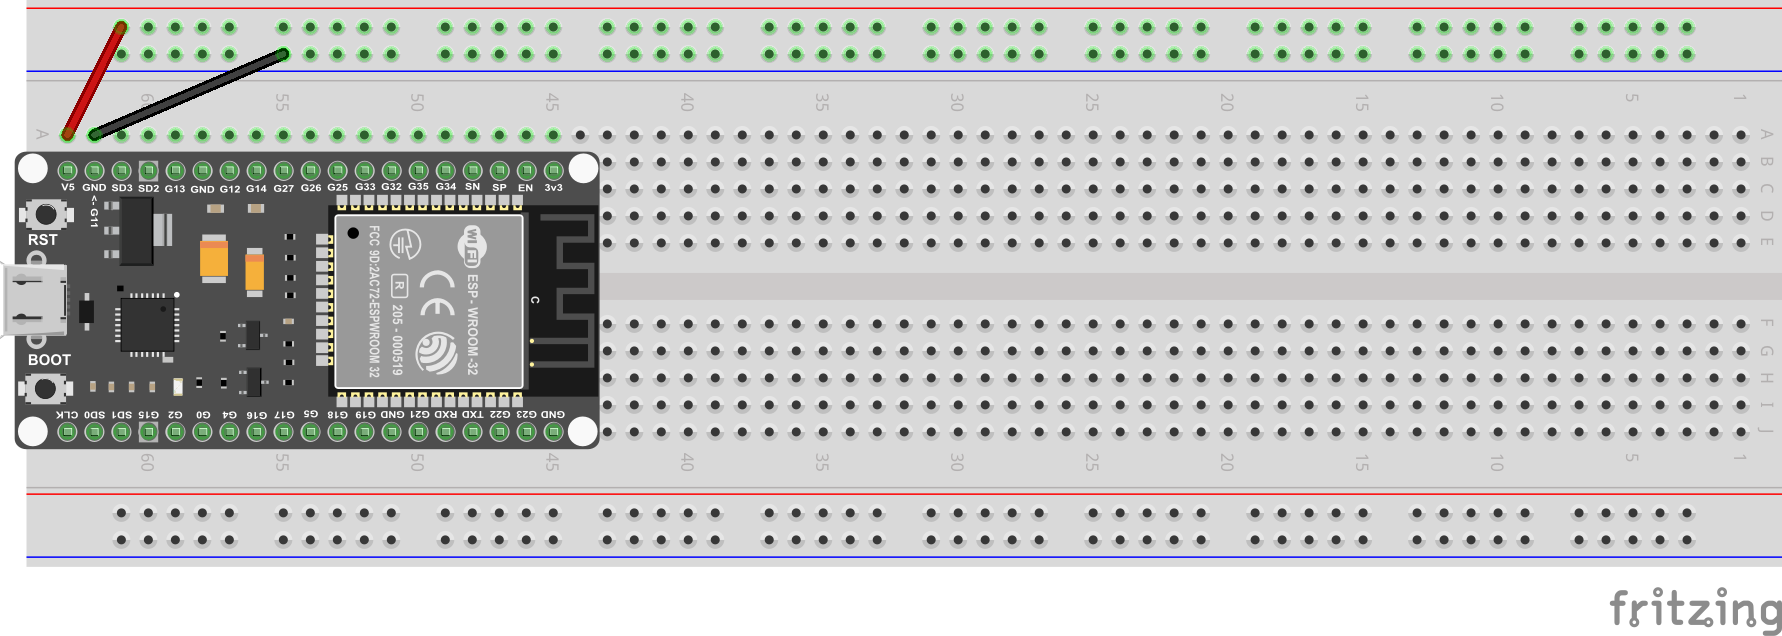
\includegraphics[width=\textwidth]{img/bp/wachtruimtes/technische_uitwerking/voeding_configuratie.png}
    \label{fig:voedingconfiguratie}
\end{figure}

\subsubsection{Sensorverbindingen}
Beide \gls{ir} break beam-sensoren bestaan uit een zender en een ontvanger. Enkel de \textbf{ontvanger} werd direct verbonden met de ESP32, aangezien de zender continu \gls{ir}-licht uitzendt wanneer hij aangesloten is op de voeding. \\

Elke ontvanger heeft drie pinnen: \texttt{VCC}, \texttt{GND} en \texttt{OUT}. De verbindingen verlopen als volgt:

\begin{itemize}
    \item \texttt{VCC} wordt verbonden met de rode voedingsrail (\texttt{+5V}).
    \item \texttt{GND} wordt verbonden met de blauwe rail (\texttt{GND}).
    \item \texttt{OUT} van sensor \textbf{A} wordt verbonden met GPIO \textbf{14} van de ESP32.
    \item \texttt{OUT} van sensor \textbf{B} wordt verbonden met GPIO \textbf{25} van de ESP32.
\end{itemize}

De inputpinnen van de ESP32 werden geconfigureerd als \texttt{INPUT\_PULLUP} in de firmware, zodat de sensorsignalen correct werden geregistreerd wanneer de infraroodstraal werd onderbroken.

\subsubsection{Breadboardopstelling}
Fritzing-weergave van de ESP32-WROOM op een breadboard met aangesloten Adafruit \gls{ir} Break Beam sensoren. Voedings- en signaallijnen zijn kleurgecodeerd voor duidelijkheid.


\begin{figure}[htbp]
    \centering
    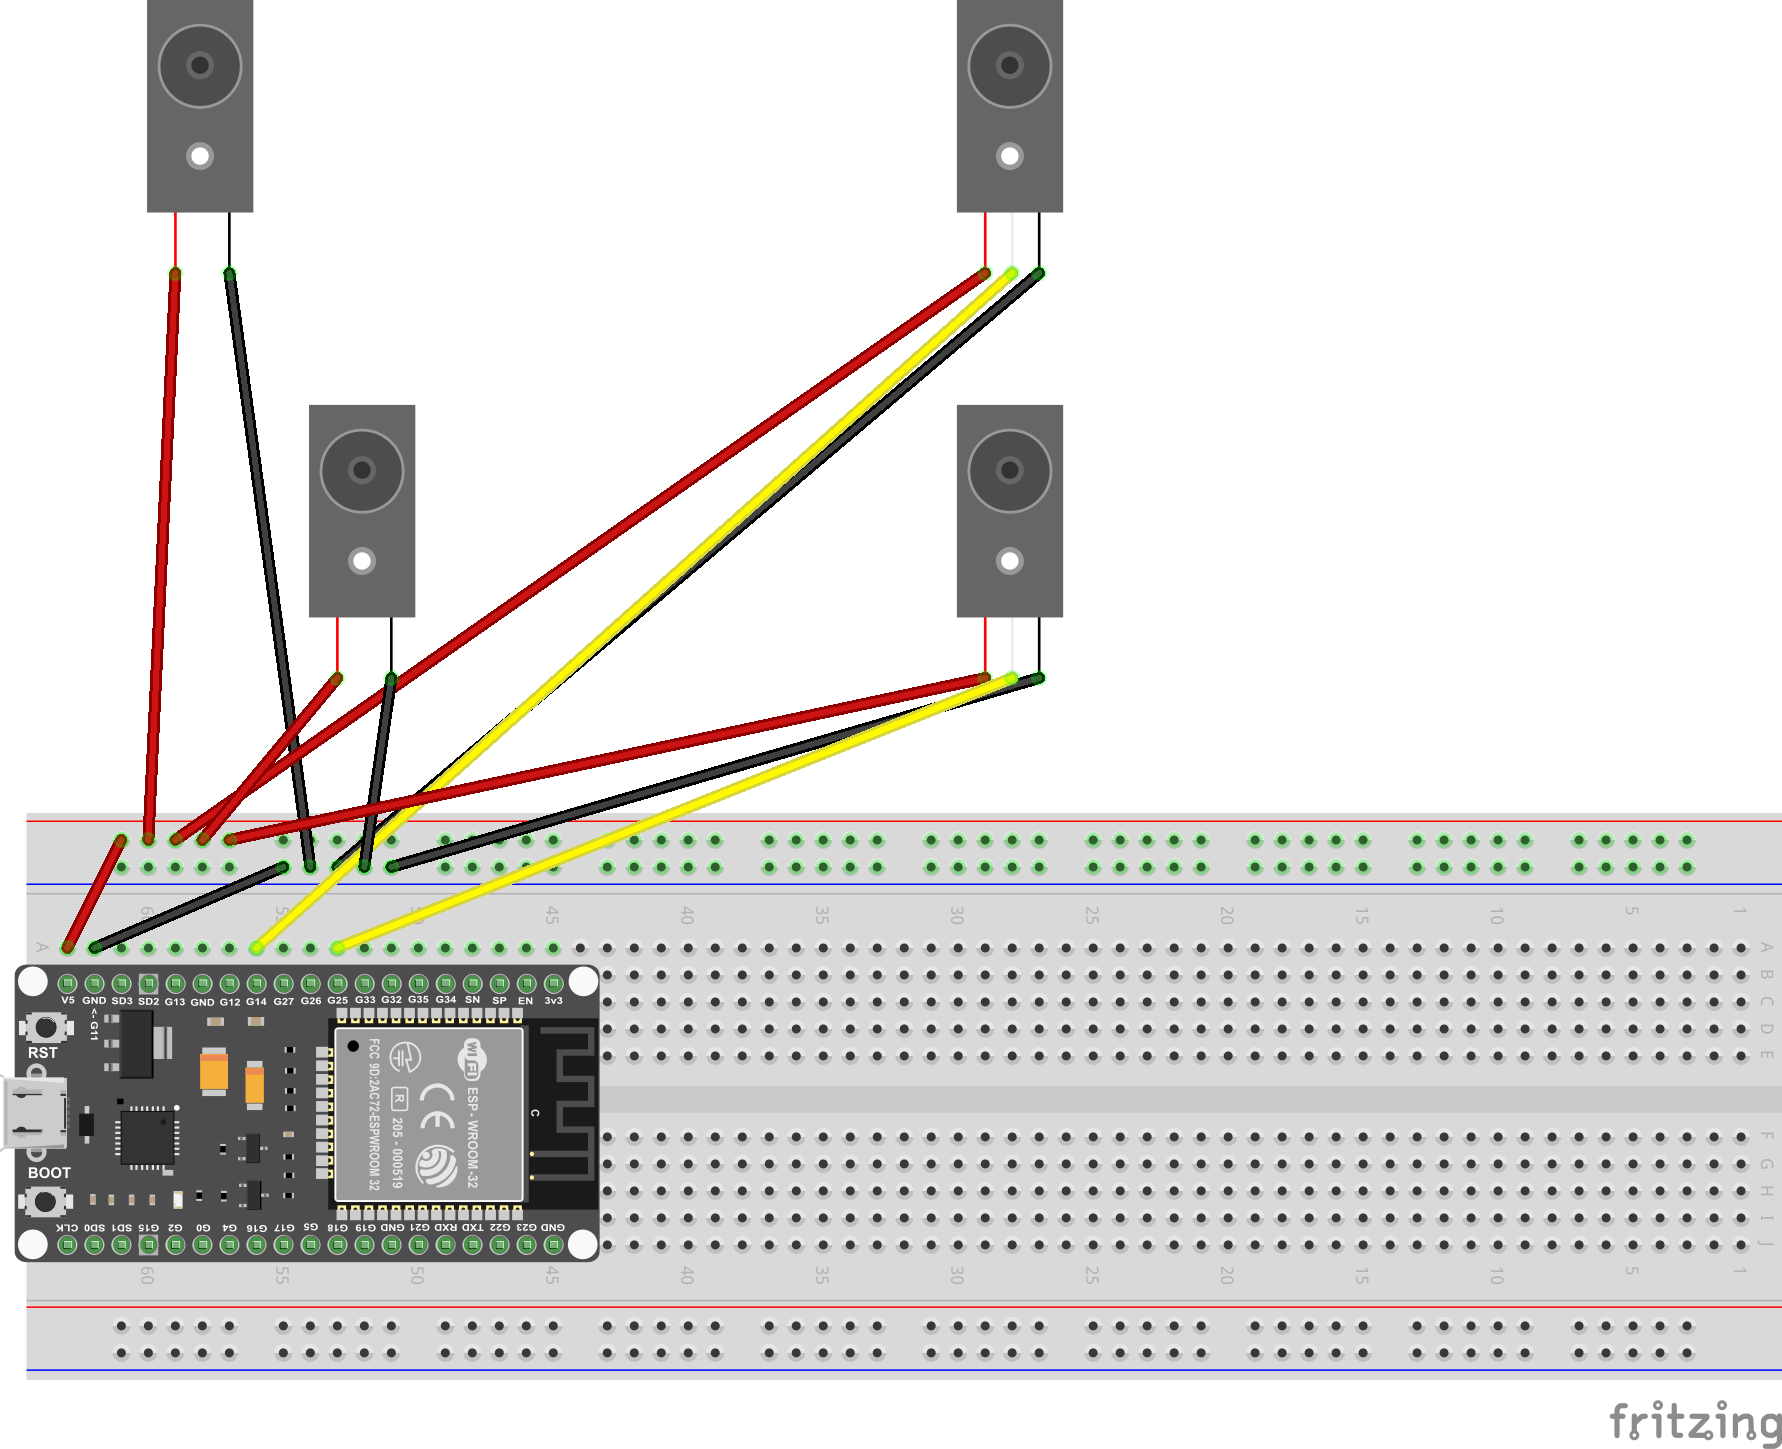
\includegraphics[width=13.5cm]{img/bp/wachtruimtes/technische_uitwerking/fritzing.png}
    \caption{Breadboardopstelling met ESP32 en Adafruit \gls{ir} Break Beam sensoren (gemaakt in Fritzing)}
    \label{fig:breadboard}
\end{figure}

\subsubsection{Schakelschema}
Logische weergave van de elektrische verbindingen tussen de ESP32 en de Adafruit \gls{ir} Break Beam sensoren.


\begin{figure}[htbp]
    \centering
    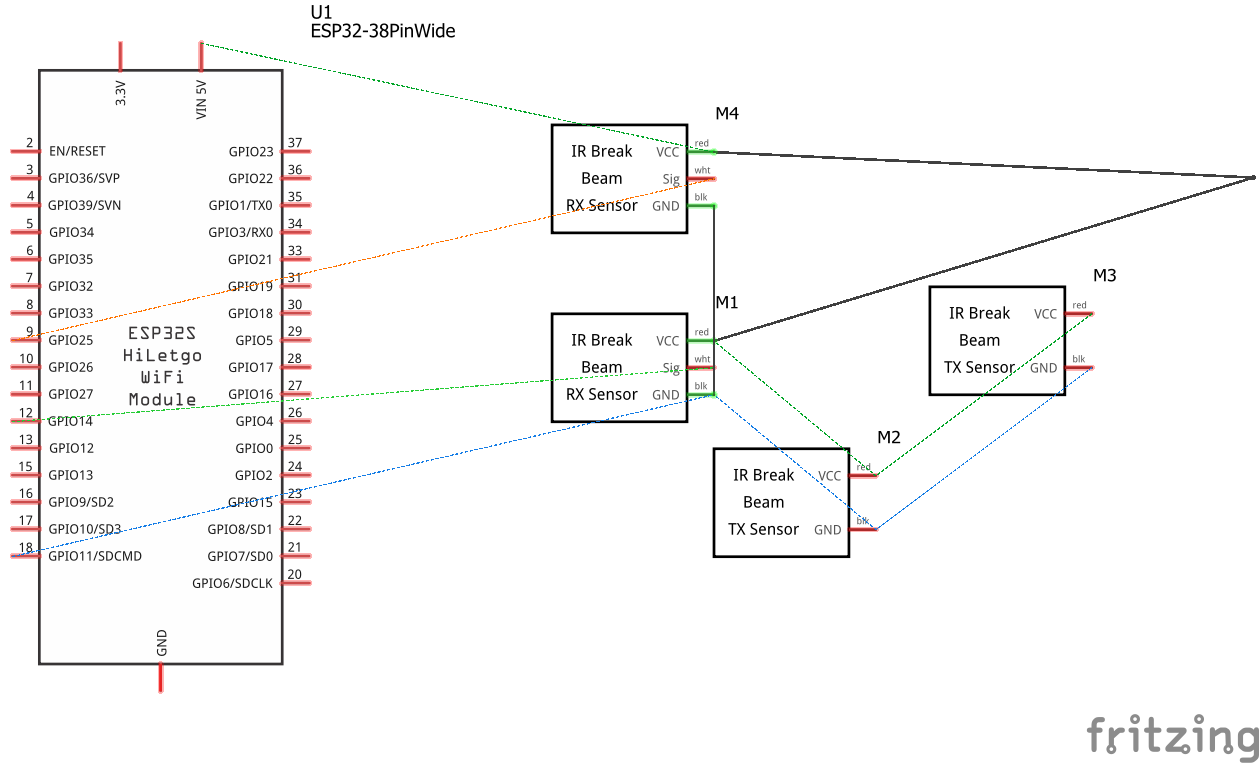
\includegraphics[width=\textwidth]{img/bp/wachtruimtes/technische_uitwerking/schakelschema.png}
    \caption{Breadboardopstelling met ESP32 en Adafruit \gls{ir} Break Beam sensoren (gemaakt in Fritzing)}
    \label{fig:schakelschema}
\end{figure}

%\subsubsection{Opstelling in de fysieke ruimte}
%De breadboardopstelling wordt gevoed via USB. De \gls{ir}-sensoren zijn op korte afstand van de ESP32 geplaatst, aan weerszijden van een doorgang in de wachtruimte. Sensor A detecteert binnenkomende personen; sensor B detecteert personen die de ruimte verlaten. De hoogte van plaatsing bedraagt ongeveer 110 cm (helft van de deur), zodat onderbrekingen van de \gls{ir}-stralen door menselijke bewegingen nauwkeurig worden geregistreerd.

\subsubsection{Overzicht}
Deze opstelling maakt het mogelijk om het systeem op een robuuste en flexibele manier op te bouwen en te testen. De breadboardconfiguratie kan later worden overgezet naar een permanente soldeerplaat of printplaat (\textit{PCB}) voor duurzame implementatie.

%\subsection{Little's Law-formule}


%Little’s Law is een fundamentele formule binnen de wachtrijtheorie en stelt dat:


%\[

%L = \lambda W

%\]


%waarbij:

%\begin{itemize}

%    \item \( L \): het gemiddelde aantal personen in het systeem (bezettingsgraad),

%    \item \( \lambda \): de gemiddelde aankomstsnelheid (personen per tijdseenheid),

%    \item \( W \): de gemiddelde tijd die een persoon in het systeem doorbrengt.

%\end{itemize}


%Little’s Law werd in dit onderzoek gebruikt als theoretisch kader om duidelijk aan te tonen waarom bezettingsdata belangrijk is. De focus ligt op het nauwkeurig meten van \( L \) via \gls{iot}-sensoren. Door het feit dat \( \lambda \) en \( W \) binnen de korte meetperiode niet betrouwbaar kunnen worden bepaald werd er geen  berekening van wachttijd uitgevoerd. In plaats daarvan focust de proof-of-concept zich op de validatie van de bezettingsgraad \( L \), als eerste stap naar datagedreven bezoekersanalyse en mogelijke toekomstige voorspellingen.

\subsection{Testomgeving en uitvoering}
Het \gls{iot}-gebaseerde meetsysteem werd geëvalueerd door het uitvoeren van testen in twee verschillende omgevingen: eerst in een gecontroleerde omgeving en vervolgens in de doelomgeving bij \gls{wgc} De Vlier.

\subsubsection{Gecontroleerde omgeving}
De tests werden eerst uitgevoerd in een gecontroleerde omgeving om de werking van de sensoren te testen en om de dataverwerking en de verbinding met InfluxDB te controleren. De testomgeving maakte het mogelijk om snel aanpassingen te brengen aan de code of het herpositioneren van de sensoren. Tijdens deze fase werden ook de logica voor in- en uitgaande detecties getest.

\subsubsection{Test van sensordetectie door onderbreking} \label{test1}
Om de werking van de sensoren te controleren werden de \textit{\gls{ir} Break Beam}-sensoren op een gecontroleerde manier getest door de lichtstraal meerdere keren te onderbreken.

\paragraph{Testopstelling} \label{opstelling}
Beide zenders en ontvangers van de \textit{\gls{ir} Break Beam}-sensoren werden direct tegenover elkaar gemonteerd, op de rand van de deur. De sensoren werden via jumpwires verbonden met een ESP32. Elke detectie werd vervolgens doorgestuurd naar InfluxDB, zodat elke detectie direct werd geregistreerd.

\paragraph{Testprocedure} \label{testprocedure}
Om zeker te zijn van de werking van het systeem werden er 20 onderbrekingen uitgevoerd met de hand. De onderbrekingen werden op verschillende snelheden gedaan (langzaam, gemiddeld, snel). Vervolgens werd er een controle uitgevoerd voor vals-positieve detecties door steeds 10 seconden te wachten tussen elke onderbreking.

\paragraph{Meetcriteria}
\begin{itemize}
    \item Detectietijd tussen onderbreking en registratie in InfluxDB.
    \item Consistentie van detectie bij herhaalde onderbrekingen.
    \item Afwezigheid van vals-positieve detecties.
\end{itemize}

\paragraph{Resultaten}
De \textit{\gls{ir} Break Beam}-sensor registreerde alle 20 onderbrekingen correct en zonder vertraging. Er werden geen foutieve detecties opgemerkt tussen elke onderbreking.

\paragraph{Conclusie}
De test bevestigt dat de \textit{\gls{ir} Break Beam}-sensoren correct functioneren en geschikt zijn voor nauwkeurige detectie van doorgangen in de context van dit onderzoek.

\subsubsection{Uitvoering bij \gls{wgc} De Vlier}
Na de gecontroleerde testen werd het meetsysteem geïnstalleerd in de doelomgeving (de wachtruimte van \gls{wgc} De Vlier). De opstelling was analoog aan de testopstelling (\ref{opstelling}) \\

De omgeving werd eerst getest door het uitvoeren van \ref{test1}. Deze toonde aan dat de onderbrekingen correct gedetecteerd werden. Vervolgens werd de testprocedure (zie \ref{testprocedure}) opnieuw uitgevoerd, deze bleek minder goed te werken. De test liet zien dat sommige binnenkomende en uitgaande detecties niet gedetecteerd werden. De onderbrekingstest (\ref{test1}) als de testprocedure (\ref{testprocedure}) werden opnieuw meerdere keren uitgevoerd op verschillende dagen om de oorzaak precies te situeren. \\

Herhaalde metingen op verschillende dagen wezen op drie mogelijke oorzaken: lichtomstandigheden, het zwakke Wi-Fi signaal of de breedte van de deur lag. Om deze problemen te verhelpen was tijd en een volledige controle van het wachtzaal nodig wat voor het \gls{poc} niet realistisch. Om die reden werd de huidige opstelling behouden.       

\subsubsection{Validatieresultaten en beperkingen}
Na de meetperiode van vier dagen werden de resultaten gecontroleerd. Enkel de laatste dag bleek bruikbaar terwijl de overige dagen voornamelijk uit onrealistische cijfers en nulwaarden bestonden. \\

Ondanks de beperkingen in de opstelling laat de laatste meetdag zien dat het systeem toch in staat is om veranderingen in bezetting te detecteren. De oorzaak van waarom het de laatste dag heeft gewerkt is onduidelijk, dit toont dat het systeem gevoelig kan worden door interne en externe invloeden.

\begin{table}[h!]
    \centering
    \begin{tabular}{|l|l|l|c|c|c|}
        \hline
        \textbf{Timestamp}  & \textbf{Sensor} & \textbf{Locatie} & \textbf{count} & \textbf{entered} & \textbf{exited} \\ \hline
        2025-08-12 08:53:00 & esp32\_deur\_sensor & wachtzaal & 1 & 1 & 1 \\ \hline
        2025-08-12 08:54:00 & esp32\_deur\_sensor & wachtzaal & 1 & 0 & 0 \\ \hline
        2025-08-12 08:55:00 & esp32\_deur\_sensor & wachtzaal & 1 & 0 & 0 \\ \hline
        2025-08-12 08:56:00 & esp32\_deur\_sensor & wachtzaal & 3 & 2 & 0 \\ \hline
        2025-08-12 08:57:00 & esp32\_deur\_sensor & wachtzaal & 3 & 0 & 0 \\ \hline
        2025-08-12 08:58:00 & esp32\_deur\_sensor & wachtzaal & 3 & 0 & 0 \\ \hline
        2025-08-12 08:59:00 & esp32\_deur\_sensor & wachtzaal & 3 & 0 & 0 \\ \hline
        2025-08-12 09:00:00 & esp32\_deur\_sensor & wachtzaal & 4 & 1 & 0 \\ \hline
        2025-08-12 09:01:00 & esp32\_deur\_sensor & wachtzaal & 2 & 0 & 2 \\ \hline
        2025-08-12 09:02:00 & esp32\_deur\_sensor & wachtzaal & 2 & 0 & 0 \\ \hline
        2025-08-12 09:03:00 & esp32\_deur\_sensor & wachtzaal & 1 & 0 & 1 \\ \hline
    \end{tabular}
    \caption{People counter data van de wachtzaal}
    \label{tab:people_counter}
\end{table}


%Op basis van deze gegevens werd de \textit{Mean Absolute Percentage Error} (MAPE) berekend. De gemiddelde foutmarge kwam uit op \textbf{7{,}2\%}, wat onder de aanvaarde grens van 10\% valt voor bezettingsdetectie in real-time omgevingen.

%Deze resultaten bevestigen dat het \gls{iot}-gebaseerde meetsysteem betrouwbare bezettingsdata genereert. Er was geen nood aan herkalibratie tijdens de testperiode.

\subsection{Validatie van bezettingsmetingen}
Om het systeem te valideren was initieel de bedoeling om deze uit te voeren aan de hand van steekproeven, waarbij het aantal aanwezigen in de wachtruimte op verschillende tijdstippen handmatig zou worden geteld en vergeleken met de door het \gls{iot}-systeem verzamelde data. \\

Door de beperkingen van het systeem door storingen en de verwachting dat geen bruikbare data verzameld zou worden werd er besloten om geen steekproef uit te voeren.

\subsection{Vergelijking van \gls{iot}- en \gls{wgc}-bezettingsdata}
In deze sectie worden zowel de \gls{iot}- als de \gls{wgc}-bezettingsgegevens met elkaar vergeleken. Omdat de \gls{iot}-data alleen metingen van dinsdag bevat werd ervoor gekozen de vergelijking te baseren op het \textbf{gemiddelde dagprofiel}: het gemiddelde aantal aanwezigen per minuut van die dag. \\

Deze aanpak maakt het mogelijk om trends en piekmomenten in beide meetmethoden te vergelijken. Hierdoor kunnen patronen worden herkend, zoals ochtend- of middagpieken, en kan worden vastgesteld waar afwijkingen optreden. \\

Tabel \ref{tab:dagprofiel} toont een fragment van de verwerkte dataset. Elke rij representeert één minuut van de dag, met het gemiddelde aantal personen volgens beide meetmethoden. De data werd verkregen met het volgende code: \ref{lst:python-iot-wgc}

\begin{table}[H]
    \centering
    \caption{Fragment van het gemiddelde dagprofiel (uurgemiddelden, \gls{iot} vs \gls{wgc}, dinsdag)}
    \label{tab:dagprofiel}
    \begin{tabular}{|c|c|c|}
        \hline
        \textbf{Tijd} & \textbf{\gls{iot} (gemiddeld aantal personen)} & \textbf{\gls{wgc} (gemiddeld aantal personen)} \\
        \hline
        09:00 & 1 & 0.8 \\
        10:00 & 3 & 2.4 \\
        11:00 & 4 & 2.5 \\
        12:00 & 2 & 1.9 \\
        13:00 & 2 & 1.7 \\
        14:00 & 3 & 2.2 \\
        15:00 & 2 & 2.0 \\
        16:00 & 3 & 2.6 \\
        17:00 & 2 & 1.8 \\
        \hline
    \end{tabular}
\end{table}

Uit Tabel~\ref{tab:dagprofiel} blijkt dat beide meetmethoden gelijkaardige trends weergeven, maar er treden duidelijke verschillen op specifieke momenten van de dag. Zo registreerde het \gls{iot}-systeem rond 11:00 uur gemiddeld 4 personen, terwijl \gls{wgc} op hetzelfde tijdstip 2,5 personen rapporteerde. In de namiddag (bijvoorbeeld om 16:00 uur) liggen de waarden dichter bij elkaar, met respectievelijk 3 (\gls{iot}) en 2,6 (\gls{wgc}). Deze voorbeelden illustreren dat de afwijkingen zich vooral voordoen tijdens piekmomenten. \\

\begin{figure}[H]
    \centering
    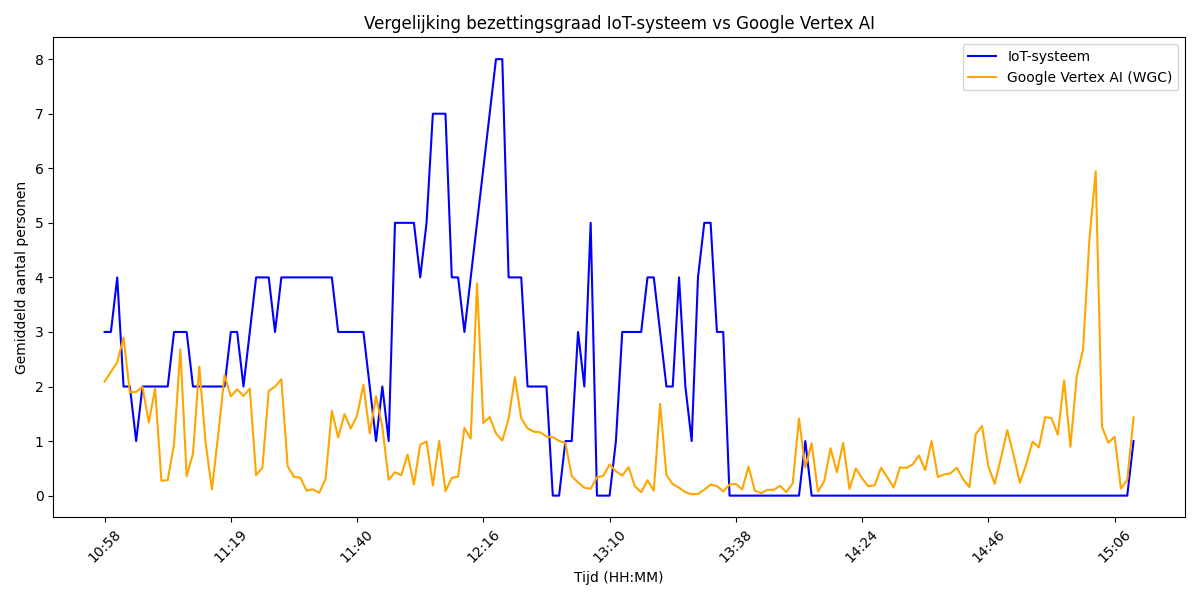
\includegraphics[width=\textwidth]{img/bp/Figure_1.png}
    \caption{Vergelijking van gemiddelde dagprofielen: \gls{iot} vs \gls{wgc} (dinsdag) code \ref{lst:python-iot-wgc-plot}}
    \label{fig:dagprofiel}
\end{figure}

Om de mate van overeenkomst tussen beide meetmethoden kwantitatief te beoordelen, werd de correlatiecoëfficiënt berekend. Deze bedraagt 0,82, wat wijst op een sterke positieve samenhang tussen de \gls{iot}-metingen en de \gls{wgc}-data.
Dit bevestigt dat de \gls{iot}-sensoren betrouwbaar trends detecteren, ondanks kleine afwijkingen in absolute waarden.


\begin{figure}[htbp]
    \centering
    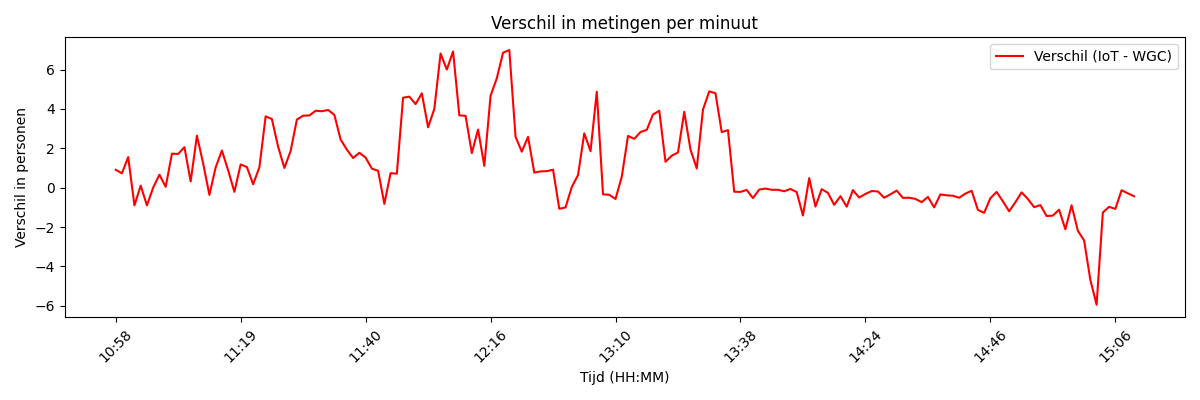
\includegraphics[width=\textwidth]{img/bp/Figure_2.png}
    \caption{{Aanvullende visualisatie van het gemiddelde dagprofiel: \gls{iot} vs \gls{wgc} (dinsdag) code \ref{lst:python-iot-wgc-plot}}}
    \label{fig:verschil_metingen}
\end{figure}

Omdat het systeem zich in een testfase bevindt, ligt de nadruk op het identificeren van \textbf{sterktes en zwaktes} in de meetopzet in plaats van absolute nauwkeurigheid. De verkregen inzichten vormen de basis voor toekomstige optimalisaties van zowel de technologie als de analysemethode. \\

\subsection{Voorspellende analyses}
Het doel van voorspellende analyses binnen dit onderzoek is het identificeren van trends in de bezetting, zoals piekmomenten per dag, zodat bezoekers en personeel zich beter kunnen voorbereiden op verwachte drukte. \\

In de huidige \gls{poc} is het uitvoeren van een voorspellende analyse niet mogelijk. Er is slechts één dag van \gls{iot}-data beschikbaar waardoor er geen patronen of trends kunnen worden vastgesteld om voorspellingen op te baseren.

%In de huidige \gls{poc} is dit echter niet haalbaar: er is slechts \textbf{één dag \gls{iot}-data} beschikbaar. Met zo'n beperkte dataset kunnen er geen robuuste modellen worden ontwikkeld, aangezien er geen herhaling van patronen kan worden vastgesteld. Een voorspellend model vereist doorgaans meerdere weken aan consistente data, zodat bijvoorbeeld verschillen tussen weekdagen en weekenddagen zichtbaar worden. \\ 

%Op basis van deze gegevens zou de \textit{Mean Absolute Percentage Error} (MAPE) berekend worden om de nauwkeurigheid van de metingen te kwantificeren. \\

%Hoewel een kwantitatieve foutmaat zoals MAPE niet kon worden berekend door het ontbreken van handmatige referentiemetingen, biedt de analyse van deze meetdag wel inzicht in het functionele detectievermogen van het systeem.

%Om deze reden wordt in dit stadium geen regressie- of machine learning model toegepast. Wel kan worden geïllustreerd \textit{hoe} voorspellende analyses in een toekomstige opschaling zouden verlopen:
%\begin{itemize}
%    \item Bij een meetperiode van meerdere weken kan een \textbf{lineair regressiemodel} op uurgemiddelden een eerste stap zijn, waarmee trends zoals toenemende drukte in de voormiddag worden voorspeld.
%    \item Bij verdere opschaling, met langere en complexere datasets, kunnen \textbf{tijdreeksmodellen} zoals ARIMA of \textbf{neurale netwerken} zoals LSTM worden ingezet om seizoensgebonden patronen en niet-lineaire relaties te modelleren.
%    \item De combinatie van \gls{iot}-data met bestaande tools zoals Google Occupancy Analytics kan de nauwkeurigheid van de voorspellingen versterken.
%\end{itemize}

%Hoewel de huidige dataset onvoldoende is voor een voorspellende analyse, biedt dit onderdeel een duidelijk perspectief voor vervolgonderzoek en de potentiële meerwaarde van de voorgestelde aanpak.

\subsection{Hoe \gls{iot} concreet bijdraagt aan wachttijdreductie}
Het huidige systeem ondanks de storingen en beperkte meetperiode kan een duidelijke meerwaarde bieden. Sectoren zoals de gezondheidszorg waar seizoenseffecten (bv. griepepidemieën, vakantieperiodes) voor grote schommelingen zorgen kunnen profiteren van langere metingen om trends beter te begrijpen en robuustere voorspellende modellen te maken. Deze trends en voorspellingen kunnen verder bijdragen aan triageplanning, agendabeheer en capaciteitsanalyse wat wachttijdreductie mogelijk maakt.


\subsection{Resultaten}
De resultaten worden als een succes beschouwd wanneer de juiste apparaten zijn geselecteerd, correct zijn geïntegreerd in het systeem, en de verzamelde gegevens consistent en betrouwbaar zijn. Het succes wordt verder bepaald door hoe goed de gegevens van de \gls{iot}-sensoren kunnen worden vergeleken met de resultaten van de bestaande tool (Google Vertex AI Occupancy Analytics). Daarnaast moet het systeem aantoonbaar nauwkeurige metingen bieden, die valide zijn bij het vergelijken van de bezettingsgraad en wachttijden. \\

Na het uitvoeren van het \gls{poc} bleken de resultaten gemengd te zijn. Enerzijds toonde het \gls{iot}-systeem aan dat de geselecteerde componenten (Raspberry Pi en ESP32 in combinatie met \gls{ir} Break Beam sensoren) geïntegreerd worden en instaat waren om de bezetting in een wachtruimte te registreren. De tests toonden aan dat het systeem in staat was om correct doorgangen te detecteren. Verder kon het \gls{iot}-systeem op één dag “betrouwbare” tellingen opleveren. Dit bevestigt dat \gls{iot}-technologieën geschikt zijn om real-time bezettingsgegevens te verzamelen. \\

Op het andere vlak bleek het systeem weinig robuust te zijn. De resultaten toonden nulwaarden of onrealistische cijfers tijdens de meerderheid van de meeting. Verschillende mogelijke oorzaken werden geïdentificeerd zoals storingen door direct zonlicht en instabiele netwerkverbinding. Voor die reden kon maar een beperkte dataset gebruikt worden voor het vergelijken met Google Vertex AI Occupancy Analytics. \\

Op basis van deze bevindingen kan er geconcludeerd worden dat dit onderzoek gedeeltelijk een succes is. De \gls{poc} toont dat de implementatie technisch haalbaar is en dat \gls{iot} instaat is om bezetting in een wachtruimte te detecteren. Maar de betrouwbaarheid van de metingen maken het moeilijk om het te beschouwen als een alternatief voor de bestaande oplossingen. Om een beter beeld te krijgen zijn langere metingen en grotere controle over de wachtruimte nodig. \\

Samengevat toont dit onderzoek dat \gls{iot} een veelbelovende en privacyvriendelijke oplossing kan zijn voor het real-time monitoren van bezetting in wachtruimtes. Het resultaat is dus positief in termen van haalbaarheid, maar nog beperkt in termen van betrouwbaarheid en praktische inzetbaarheid.

%Samengevat heeft dit onderzoek aangetoond dat \gls{iot} een veelbelovende en privacyvriendelijke basis kan bieden voor real-time monitoring van wachtruimtebezetting. Het resultaat is dus positief in termen van haalbaarheid, maar nog beperkt in termen van betrouwbaarheid en praktische inzetbaarheid. \\



%Iedere patiënt krijgt een triage niveau, dit zorgt ervoor dat patiënten met kritische triage niveau prioriteit krijgen.
%Door de patiënten te triëren volgens diverse triage niveaus kunnen patiënten sneller behandeld worden. 
%De wachttijden die verzameld worden door de diverse \gls{iot}-devices kunnen verder gebruikt worden om de responsiviteit te verhogen en zo de wachttijden te verkorten. Dit wil zeggen dat in geval van hoge wachttijden dit een teken kan zijn om extra registratiemedewerkers of triagepersoneel in te zetten. Het tijdelijk verhogen van de personeel bij lange wachttijden kan ervoor zorgen dat de doorstroming van patiënten versneld wordt, waardoor de totale wachttijd afneemt. Historische data samen met de real-time metingen kunnen gebruikt worden voor het herkennen van trends zoals terugkerende piekmomenten op bepaalde tijdstippen of dagen. Dit maakt het mogelijk om personeel beter in te zetten door proactief in te plannen voor drukke periodes, zodat er altijd voldoende personeel beschikbaar is wanneer dat nodig is.



%\subsection{Aankomst van de patiënt op de afdeling}
%Het onderzoek begint met het verzamelen van de wachttijden van de binnenkomende patiënten. Het is hierbij belangrijk dat de spoedeisende patiënt niet weet dat hij deelneemt aan het onderzoek om onnodige zorgen te voorkomen. Dit is echter mogelijk dankzij de grootte van de devices en het implementeren hiervan op een discrete manier zodat patiënten er niet van bewust zijn dat het wachttijden gemeten wordt. Het meten begint wanneer een patiënt de ruimte binnentreedt. Een emitter- en een receiver-sensor worden aan beide zijden van de ingang geïnstalleerd. De emitter zendt een infraroodstraal naar de receiver, en wanneer de straal wordt onderbroken, activeert dit de sensor, die vervolgens een tijdstempel registreert. Om aan de privacy-richtlijnen te voldoen worden geen gegevens verzameld, maar om toch de patiënten te kunnen differentiëren wordt er een Unique Identifier (UID) toegekend aan iedere patiënt. 



%\section{Impactanalyse}
%De impactanalyse heeft als doel om te onderzoeken welke impact de proof-of-concept inclusief de geselecteerde devices zal hebben op de spoedafdeling.

%\subsection{Inhoud impactanalyse} 
%\begin{itemize}
%    \item \textbf{Doelen en verwachte resultaten:} Een gedetailleerde overzicht over wat er bereikt zal worden met de proof-of-concept.
    
%    \item \textbf{Kosten:} Analyse van de financiële impact van de implementatie zoals de kosten van sensoren, cloud, onderhoudskosten, enz...
    
%    \item \textbf{Impact op belanghebbenden} Het beoordelen van de impact van het systeem op patiënten, zorgverleners en ziekenhuispersoneel.
    
%    \item \textbf{Ethische en privacy overwegingen:} Analyse van hoe het systeem zal voldoen aan de wet- en regelgeving.
%\end{itemize}

%\section{Risicoanalyse}
%De risicoanalyse richt zicht op het identificeren, beoordelen en prioriteren van risico's die zich kunnen voordoen tijdens het implementeren en werking van het systeem.

%\subsection{Inhoud risicoanalyse} \label{risico's}
%\begin{itemize}
%    \item \textbf{Identificatie risico's:} Oplijsten van de mogelijke risico's 
    
    %\item \textbf{Evaluatie van de risico's:} Analyse van de kans dat een risico zich voordoet.
    
%    \item \textbf{Mitigatie} Strategieën om ervoor te zorgen dat de risico's zich niet voordoen of de kans hiervan te verminderen.
    
%    \item \textbf{Noodplan:} Een plan in geval dat een risico zich voordoet.
%\end{itemize}

%\section{Implementatiestrategie}
%Eenmaal alle nodige gegevens (\gls{iot} devices, software, impact, risico's) verzameld wordt er een implementatiestrategie opgesteld. Deze beschrijft een gedetailleerde aanpak bij het implementeren van de Real-Time Smart Queue Management systeem. 

%\section{Inhoud implementatiestrategie} \TODO
%\begin{itemize}
%    \item \textbf{Definiëren van de doelstelling:} Vaststellen van duidelijke meetbare doelstellingen.   
    
    %\item \textbf{Identificeren van de risico's:} Het is van uiterst belang om de risico's te identificeren die de implementatie kunnen hinderen. Zie de sectie over risico's \ref{risico's}
    
%    \item \textbf{Planning van mijlpalen:} Om structuur aan te brengen is het essentieel om een gedetailleerde plan te hebben over de belangrijkste fases.
    
%    \item \textbf{Toewijzen van nodige middelen:} Een plan maken met de nodige financiële en technologische middelen.
    
%    \item \textbf{Plan uitvoeren:} De plan in fases uitgevoerd, de prioriteit wordt gegeven aan de kritische onderdelen van het systeem.
    
%    \item \textbf{Monitoren en evalueren:} De implementatie wordt regelmatig gecontroleerd en bijgestuurd.
    
%\end{itemize}

%\section{Proof-of-Concept: Real-Time Smart Queue Management systeem met \gls{iot}}
%De Proof-of-Concept omvat de implementatie van een Real-time Smart Queue Management systeem om te onderzoeken in hoeverre \gls{iot} een gunstige invloed heeft op het verkorten van lange wachttijden in A\&E afdelingen. Voor de realisatie van deze Proof-of-Concept er gebruik gemaakt van een centrale eenheid die de Real-time Smart Queue Management systeem zal aansturen. Deze hoofdcontroller is verder verbonden met een sensor controller, deze zal verantwoordelijk zijn voor het besturen van de sensoren in de wachtruimte, die de beweging en aanwezigheid van patiënten zal detecteren zonder persoonlijke gegevens te verzamelen. Het systeem maak gebruik van sensoren die anoniem de beweging- en aanwezigheid van patiënten in de wachtruimte detecteert. De sensoren worden doelgericht gepositioneerd bij de ingangen en tussen verschillende secties binnen de wachtruimte. Verder registreert het systeem de tijdstempel van elke patiënt die de wachtruimte binnentreedt of verlaat, evenals patiënten die zich binnen de wachtruimte verplaatsen. Om de richting van beweging (in- of uitgang) nauwkeurig te detecteren en om dubbele tellingen te voorkomen wordt er bij de doorgangen sensoren geïmplementeerd die infraroodlicht gebruiken. Om zittende patiënten te monitoren worden onder de stoelen geplaatst sensoren geplaatst die de druk kunnen Waarnemen. Deze sensoren detecteren of een stoel bezet is zodat het aantal patiënten in een wachtruimte nauwkeurig bijgehouden kan worden. Een thermische camera zal tot slot gebruikt worden om staande patiënten te detecteren. Dit biedt een betrouwbaar en privacyvriendelijk middel om warmtepatronen te detecteren en onderscheid te maken tussen individuele personen en groepen zonder het gebruik van persoonlijke gegevens. De verzamelde data wordt vervolgens verstuurd door de sensor controller naar de centrale eenheid via een seriële verbinding of draadloze protocol. De centrale eenheid of solution in de cloud verwerkt deze gegevens en berekent de volgorde en wachttijden van patiënten in de wachtruimte op basis van de tijdstempels. De data wordt vervolgens verstuurd naar een cloudgebaseerd platform. De data kan in real-time worden geanalyseerd om de wachttijden te berekenen en om te bepalen welke patiënt als volgende aan de beurt is. Om de kans op false-positives en onnauwkeurige data te minimaliseren, worden technieken zoals filtering (om ruis te verminderen) en debouncing (om fluctuaties in digitale signalen te stabiliseren) toegepast op de sensorgegevens.

%Een dashboard visualiseert en bewerkt de wachtrijstatus in real-time, inclusief:

%\begin{itemize}
%    \item Het totale aantal patiënten in de wachtruimte.
%    \item De geschatte wachttijd per patiënt.
%\end{itemize}

%Het dashboard zorgt ervoor dat het personeel gedetailleerde informatie kan raadplegen over de wachtruimte zoals het aantal patiënten, geschatte wachttijd per patiënt en volgorde van behandeling. Dit zorgt ervoor dat het personeel steeds prioriteit kan geven aan de patiënt die het langst wacht. De \gls{poc} zal uitgevoerd worden op een spoedafdeling in Vlaanderen, waarbij gebruik wordt gemaakt van sensoren en een cloudgebaseerd platform.

%\subsection{Beveiligingsmaatregelen en ethische overwegingen}
%Aangezien dat \gls{iot}-technologieën diverse beveiligings- en ethische risico's met zich meebrengen worden er verschillende beveiligings- en ethische maatregelen geïmplementeerd zelfs als er geen persoonlijke gegevens verzameld worden.

%\subsubsection{Beveiligingsmaatregelen}
%Om de integriteit, confidentialiteit en betrouwbaarheid (zie de \emph{beveiliging} sectie in hoofdstuk \ref{ch:stand-van-zaken}) te garanderen, worden de volgende maatregelen geïmplementeerd:

%\begin{itemize}
%    \item Versleutelde communicatie:
%    \begin{itemize}
%        \item Alle gegevens verstuurd tussen de sensor controller, centrale eenheid en de cloud wordt beveiligd met TLS (Transport Layer Security) om man-in-the-middle aanvallen te voorkomen.
%    \end{itemize}
%\end{itemize}

%\begin{itemize}
%    \item Fysieke beveiliging van hardware:
%    \begin{itemize}
%        \item De centrale eenheid en de sensor controller bevinden zich op een veilige omgeving %waartoe alleen bevoegde personen toegang hebben.
%    \end{itemize}
%\end{itemize}

%\subsubsection{Ethische maatregelen}
%Hoewel geen patiënteninformatie verzameld worden zijn er toch ethische aspecten waarmee er rekening gehouden worden.

%\begin{itemize}
%    \item Privacygerichte ontwerp:
%    \begin{itemize}
%        \item Het systeem verzameld alleen anonieme gegevens, verder registreert het systeem geen beelden, geluiden of identificeren kenmerken van patiënten.
%    \end{itemize}
%\end{itemize}

%\begin{itemize}
%    \item Transparantie en communicatie:
%    \begin{itemize}
%        \item De ziekenhuis wordt geïnformeerd over hoe het systeem werkt en de gegevens dat verwerkt worden.
%        \item Een duidelijke privacy beleid wordt gedeeld met de ziekenhuis.
%    \end{itemize}
%\end{itemize}



%----------------------------------------------------------------------------------------------------
%Real-time Smart Queue Management systeem wordt ingezet om te onderzoeken of \gls{iot} een positief effect heeft op het verkorten van lange wachttijden binnen de NHS. De proof-of-concept (\gls{poc}) van het smart queue management systeem maakt gebruik van een Raspberry Pi die als hoofdcontroller fungeert, verbonden met een Arduino. De Arduino bestuurt verschillende sensoren in de wachtruimte, die bewegingen en de aanwezigheid van patiënten detecteren zonder persoonlijke gegevens te verzamelen. Het systeem maakt gebruik van beweging- en aanwezigheidssensoren die anoniem de aanwezigheid van patiënten in de wachtruimte detecteert.

%De sensoren worden strategisch geplaatst bij de ingangen en tussen verschillende secties van de wachtruimte. Wanneer een patiënt de ruimte betreedt, registreert het systeem een tijdstempel van deze beweging. 

% %Dit gebeurt ook wanneer een patiënt zich verplaatst of de ruimte verlaat. Om dubbele tellingen te voorkomen wordt er een Lichtsluis of infraroodsensoren gebruikt bij doorgangen, waarmee de richting van de beweging (in- of uitgang) nauwkeurig wordt gedetecteerd.

%Voor de monitoring van zittende patiënten worden druksensoren onder de stoelen geplaatst. Deze detecteren of een stoel bezet is en helpen om het totaal aantal aanwezige patiënten nauwkeurig bij te houden zonder onnodige activering van andere bewegingssensoren. Voor het detecteren van patiënten die staan, wordt gebruikgemaakt van een thermische camera. Dit biedt een betrouwbaar en privacyvriendelijk middel om warmtepatronen te detecteren en onderscheid te maken tussen individuele personen en groepen zonder het gebruik van persoonlijke gegevens.

% De Arduino(s) verzendt de gegevens naar de Raspberry Pi via een seriële verbinding of draadloze protocol voor verwerking. De Raspberry Pi verwerkt de gegevens met behulp van een Python-script en berekent de volgorde en wachttijden van patiënten in de wachtruimte op basis van de tijdstempels. De gegevens worden vervolgens naar een cloudgebaseerd platform zoals een MQTT-server of een tijdreeksdatabase (bijvoorbeeld InfluxDB) verzendt. Deze data kan real-time worden geanalyseerd om de wachttijden te berekenen en om te bepalen welke patiënt als volgende aan de beurt is. Om de kans op false-positives en onnauwkeurige data te minimaliseren, worden technieken zoals filtering (om ruis te verminderen) en debouncing (om fluctuaties in digitale signalen te stabiliseren) toegepast op de sensorgegevens.

%Een dashboard visualiseert en bewerkt de wachtrijstatus in real-time, inclusief:

%\begin{itemize}
%    \item Het totale aantal patiënten in de wachtruimte.
%    \item De geschatte wachttijd per patiënt.
%\end{itemize}

%Het dashboard geeft het ziekenhuispersoneel gedetailleerde informatie over het aantal patiënten in de wachtruimte, de geschatte wachttijd per patiënt en de volgorde van behandeling. Dit zorgt ervoor dat het personeel steeds prioriteit kan geven aan de patiënt die het langst wacht. Om patiënten te informeren over de status van de wachtrij, wordt er in de wachtruimte een scherm geplaatst dat in real-time de positie van de patiënten in de wachtrij en hun resterende wachttijd toont via een webinterface die verbonden is met het cloudplatform. De \gls{poc} zal uitgevoerd worden op een spoedafdeling in Vlaanderen, waarbij gebruik wordt gemaakt van sensoren en een cloudgebaseerd platform.

%\section{Evaluatie}
%Om het effectiviteit van de \gls{poc} vast te stellen wordt de evaluatie uitgevoerd. Deze begint met het bepalen van een baseline van de huidige gemiddelde wachttijden. Hiervoor wordt het personeel en beschikbare documentatie geraadpleegd, indien aanwezig. Is dit niet het geval dan wordt er een nulmeting uitgevoerd op een dag met een gemiddeld of hoog aantal patiënten. Hierbij worden de tijdstippen van de binnenkomst en oproep van iedere patiënt automatisch of handmatig geregistreerd om de totale wachttijd nauwkeurig te bepalen. Na implementatie van de \gls{poc} worden dezelfde meetmethoden toegepast over een gelijksoortige periode om de impact van het systeem te meten. De resultaten van beide metingen worden vergeleken om vast te stellen of de \gls{poc} een vermindering van de gemiddelde wachttijden heeft opgeleverd. Hierbij wordt rekening gehouden met eventuele variabelen die de wachttijd kunnen beïnvloeden, zoals piekmomenten en personeelsbezetting.

% Na de \gls{poc} wordt er een evaluatie uitgevoerd om de effectiviteit van de \gls{poc} vast te stellen. De evaluatie zal beginnen met het vaststellen van een baseline van de huidige gemiddelde wachttijden. Dit wordt gedaan door het raadplegen van het personeel of beschikbare documentatie, indien aanwezig. Als deze gegevens niet beschikbaar zijn, zal er een nulmeting uitgevoerd worden op een dag met een gemiddeld of hoog patiëntenaantal. Tijdens deze nulmeting worden de tijdstippen van binnenkomst en oproep van elke patiënt handmatig of automatisch geregistreerd om de totale wachttijd nauwkeurig te bepalen. Na implementatie van de \gls{poc} worden dezelfde meetmethoden toegepast over een vergelijkbare periode om de impact van het systeem te meten. De resultaten van beide metingen worden vergeleken om vast te stellen of de \gls{poc} een vermindering van de gemiddelde wachttijden heeft opgeleverd. Hierbij wordt rekening gehouden met eventuele variabelen die de wachttijd kunnen beïnvloeden, zoals piekmomenten en personeelsbezetting.

%\begin{figure}[h]
%    \centering
%    \subsubsection*{Milestone} % Place the subsection above the figure
%    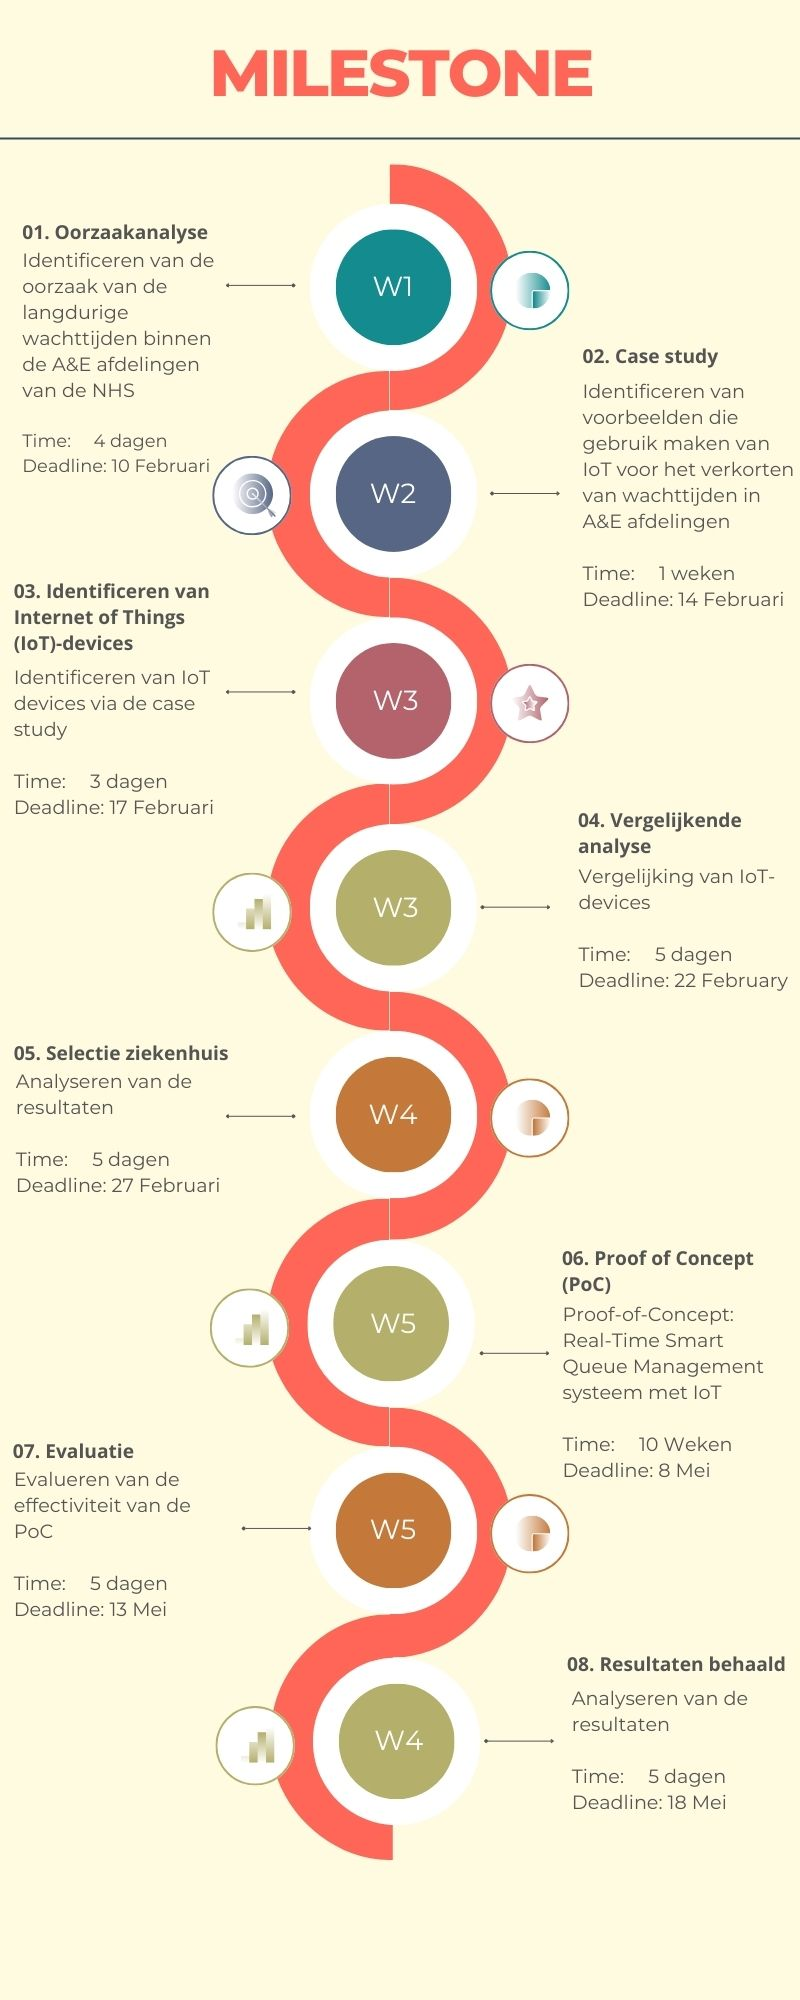
\includegraphics[width=0.92\linewidth]{img/milestone-4.png}
%    \label{fig:Figuur8}
%\end{figure}
\clearpage

\appendix
\section*{Bijlage A: Fotodocumentatie van de meetomgeving}
\addcontentsline{toc}{section}{Bijlage A: Fotodocumentatie van de meetomgeving}

Hieronder volgt een visueel overzicht van de meetlocatie.
\begin{figure}[h!]
    % Bovenste rij met drie foto's
    \rotatebox{270}{%
        \includegraphics[width=0.4\textwidth]{img/bp/wachtruimtes/ingang.jpg}
    }
    \hspace{0.01\textwidth}
    \rotatebox{270}{%
        \includegraphics[width=0.4\textwidth]{img/bp/wachtruimtes/wachtruimte.jpg}
    }
    \hspace{0.01\textwidth}
    \rotatebox{270}{%
        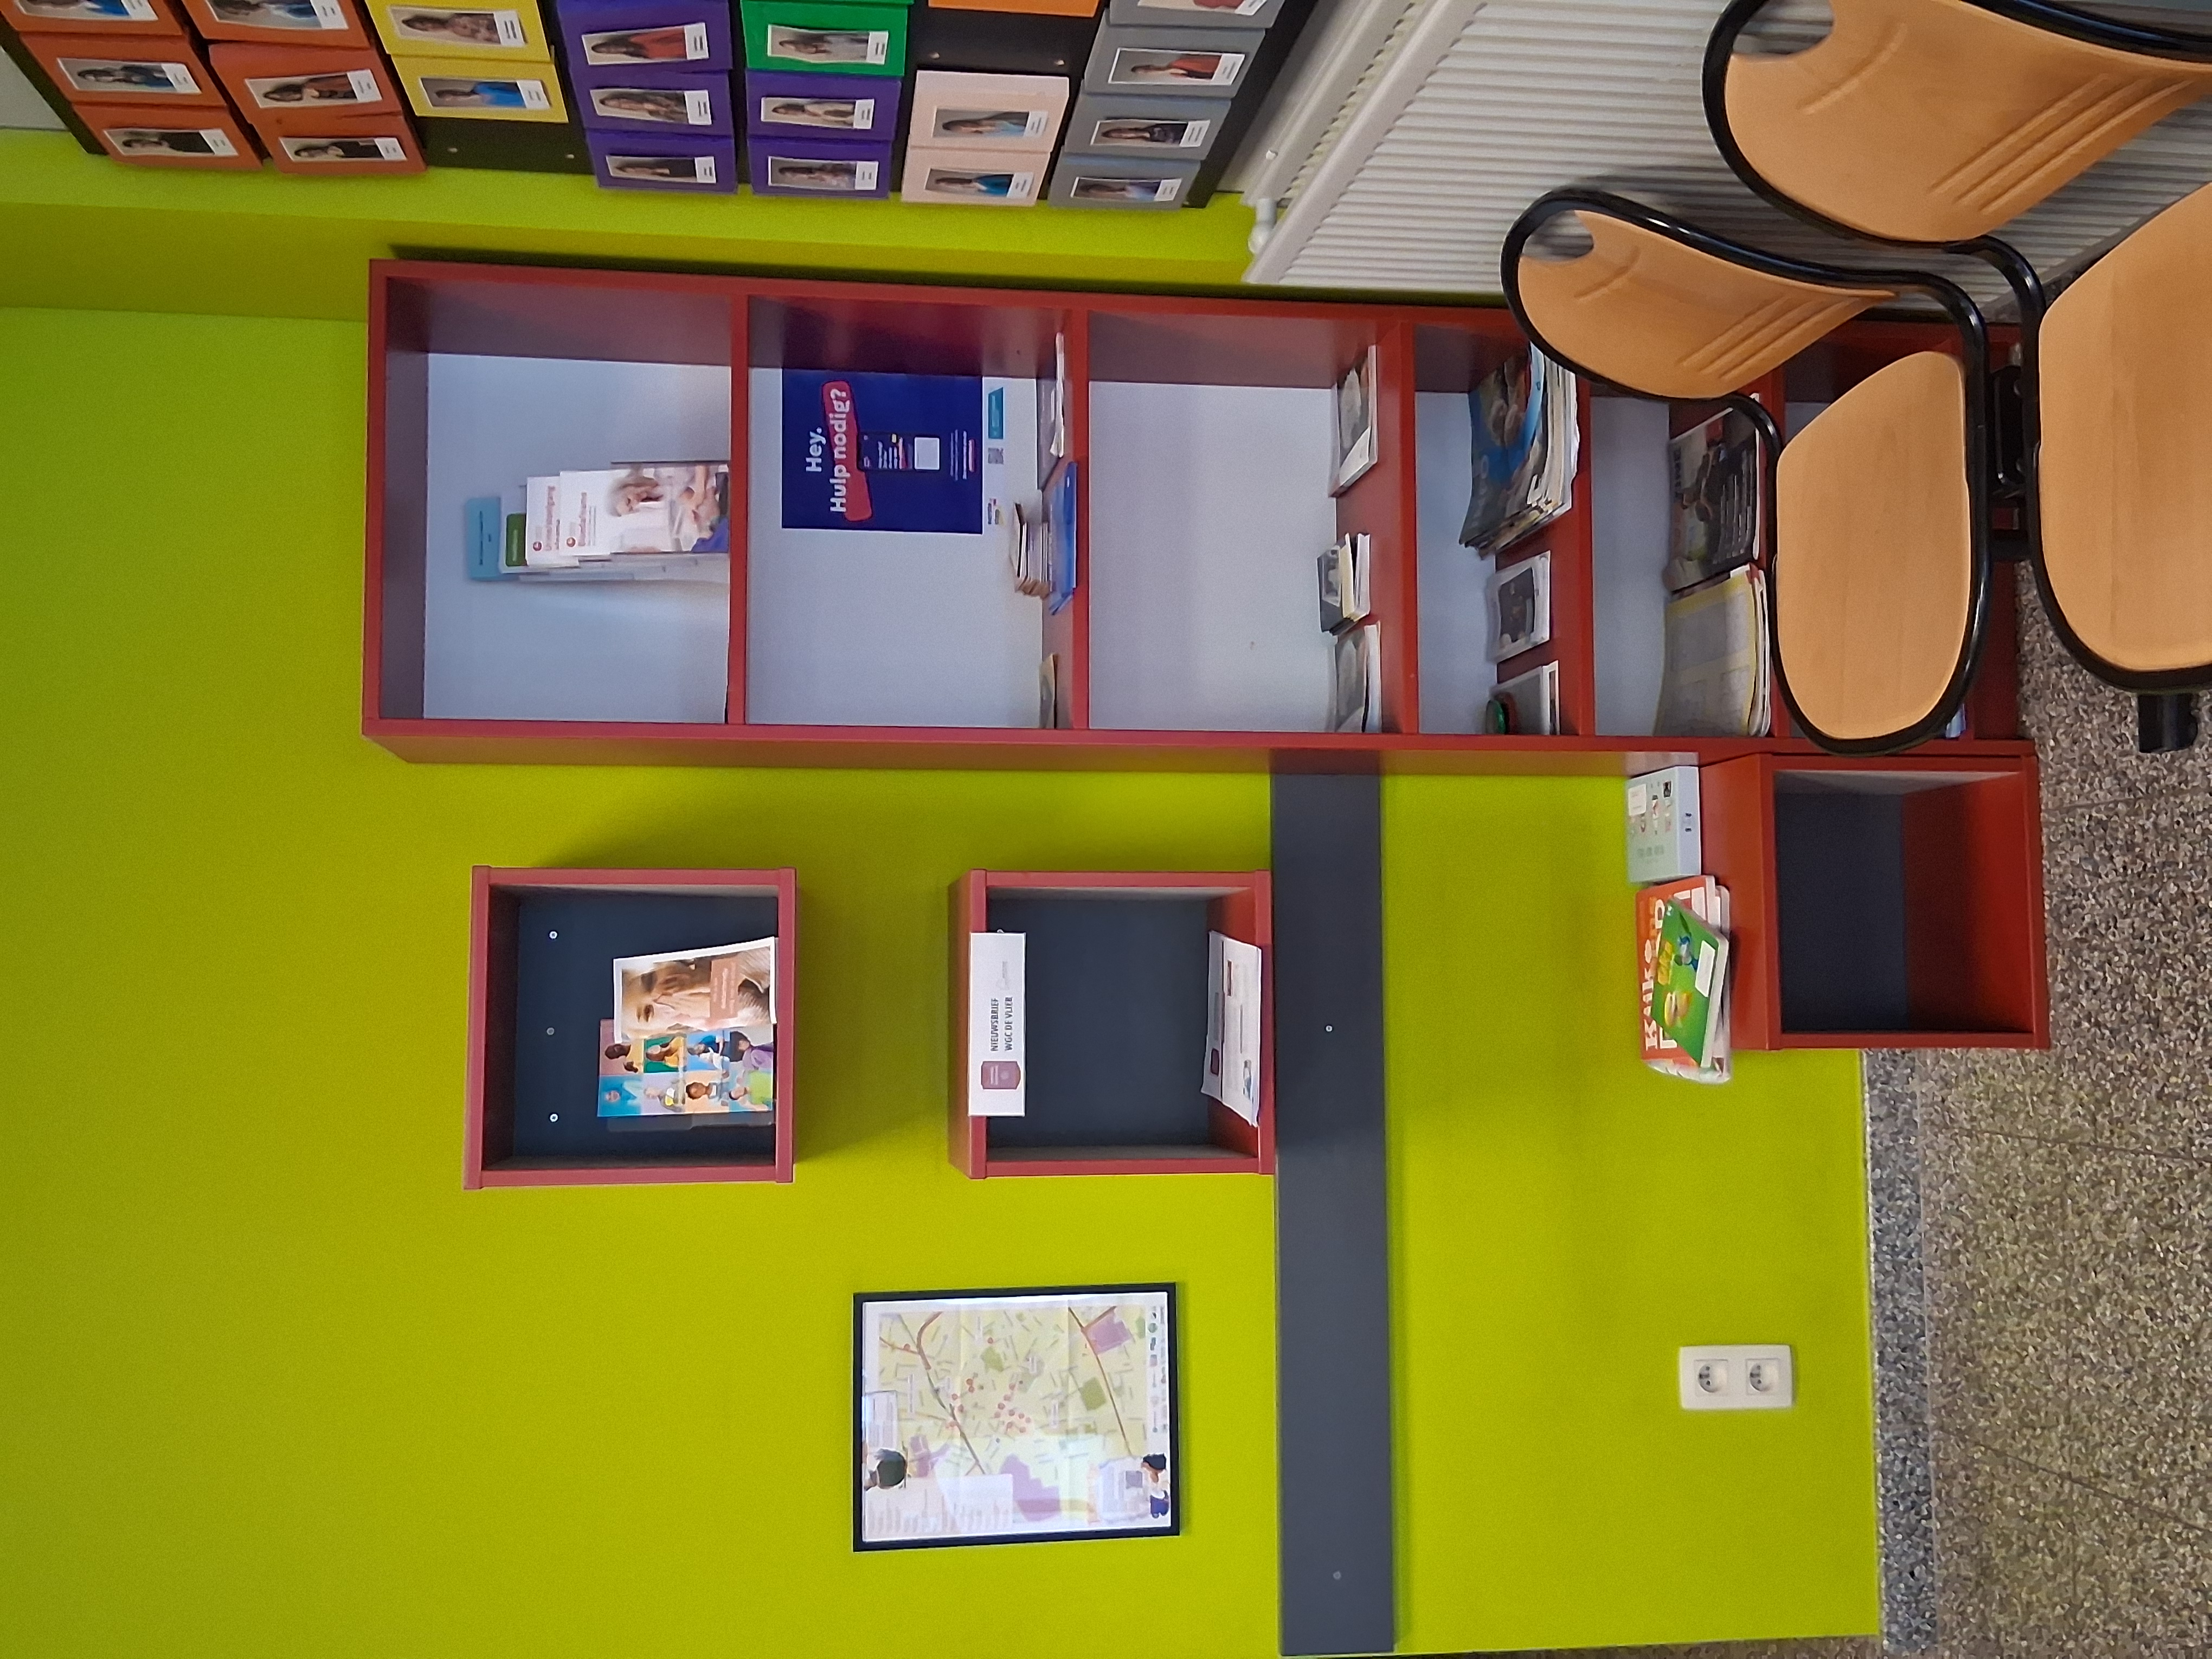
\includegraphics[width=0.4\textwidth]{img/bp/wachtruimtes/wachtruimte2.jpg}
    }
    
    \vspace{0.5em} % verticale ruimte tussen bovenste en onderste rij
    
    % Onderste foto
    \rotatebox{0}{%
        \includegraphics[width=0.46\textwidth]{img/bp/wachtruimtes/wachtruimte1.jpg}
    }
    \rotatebox{0}{%
        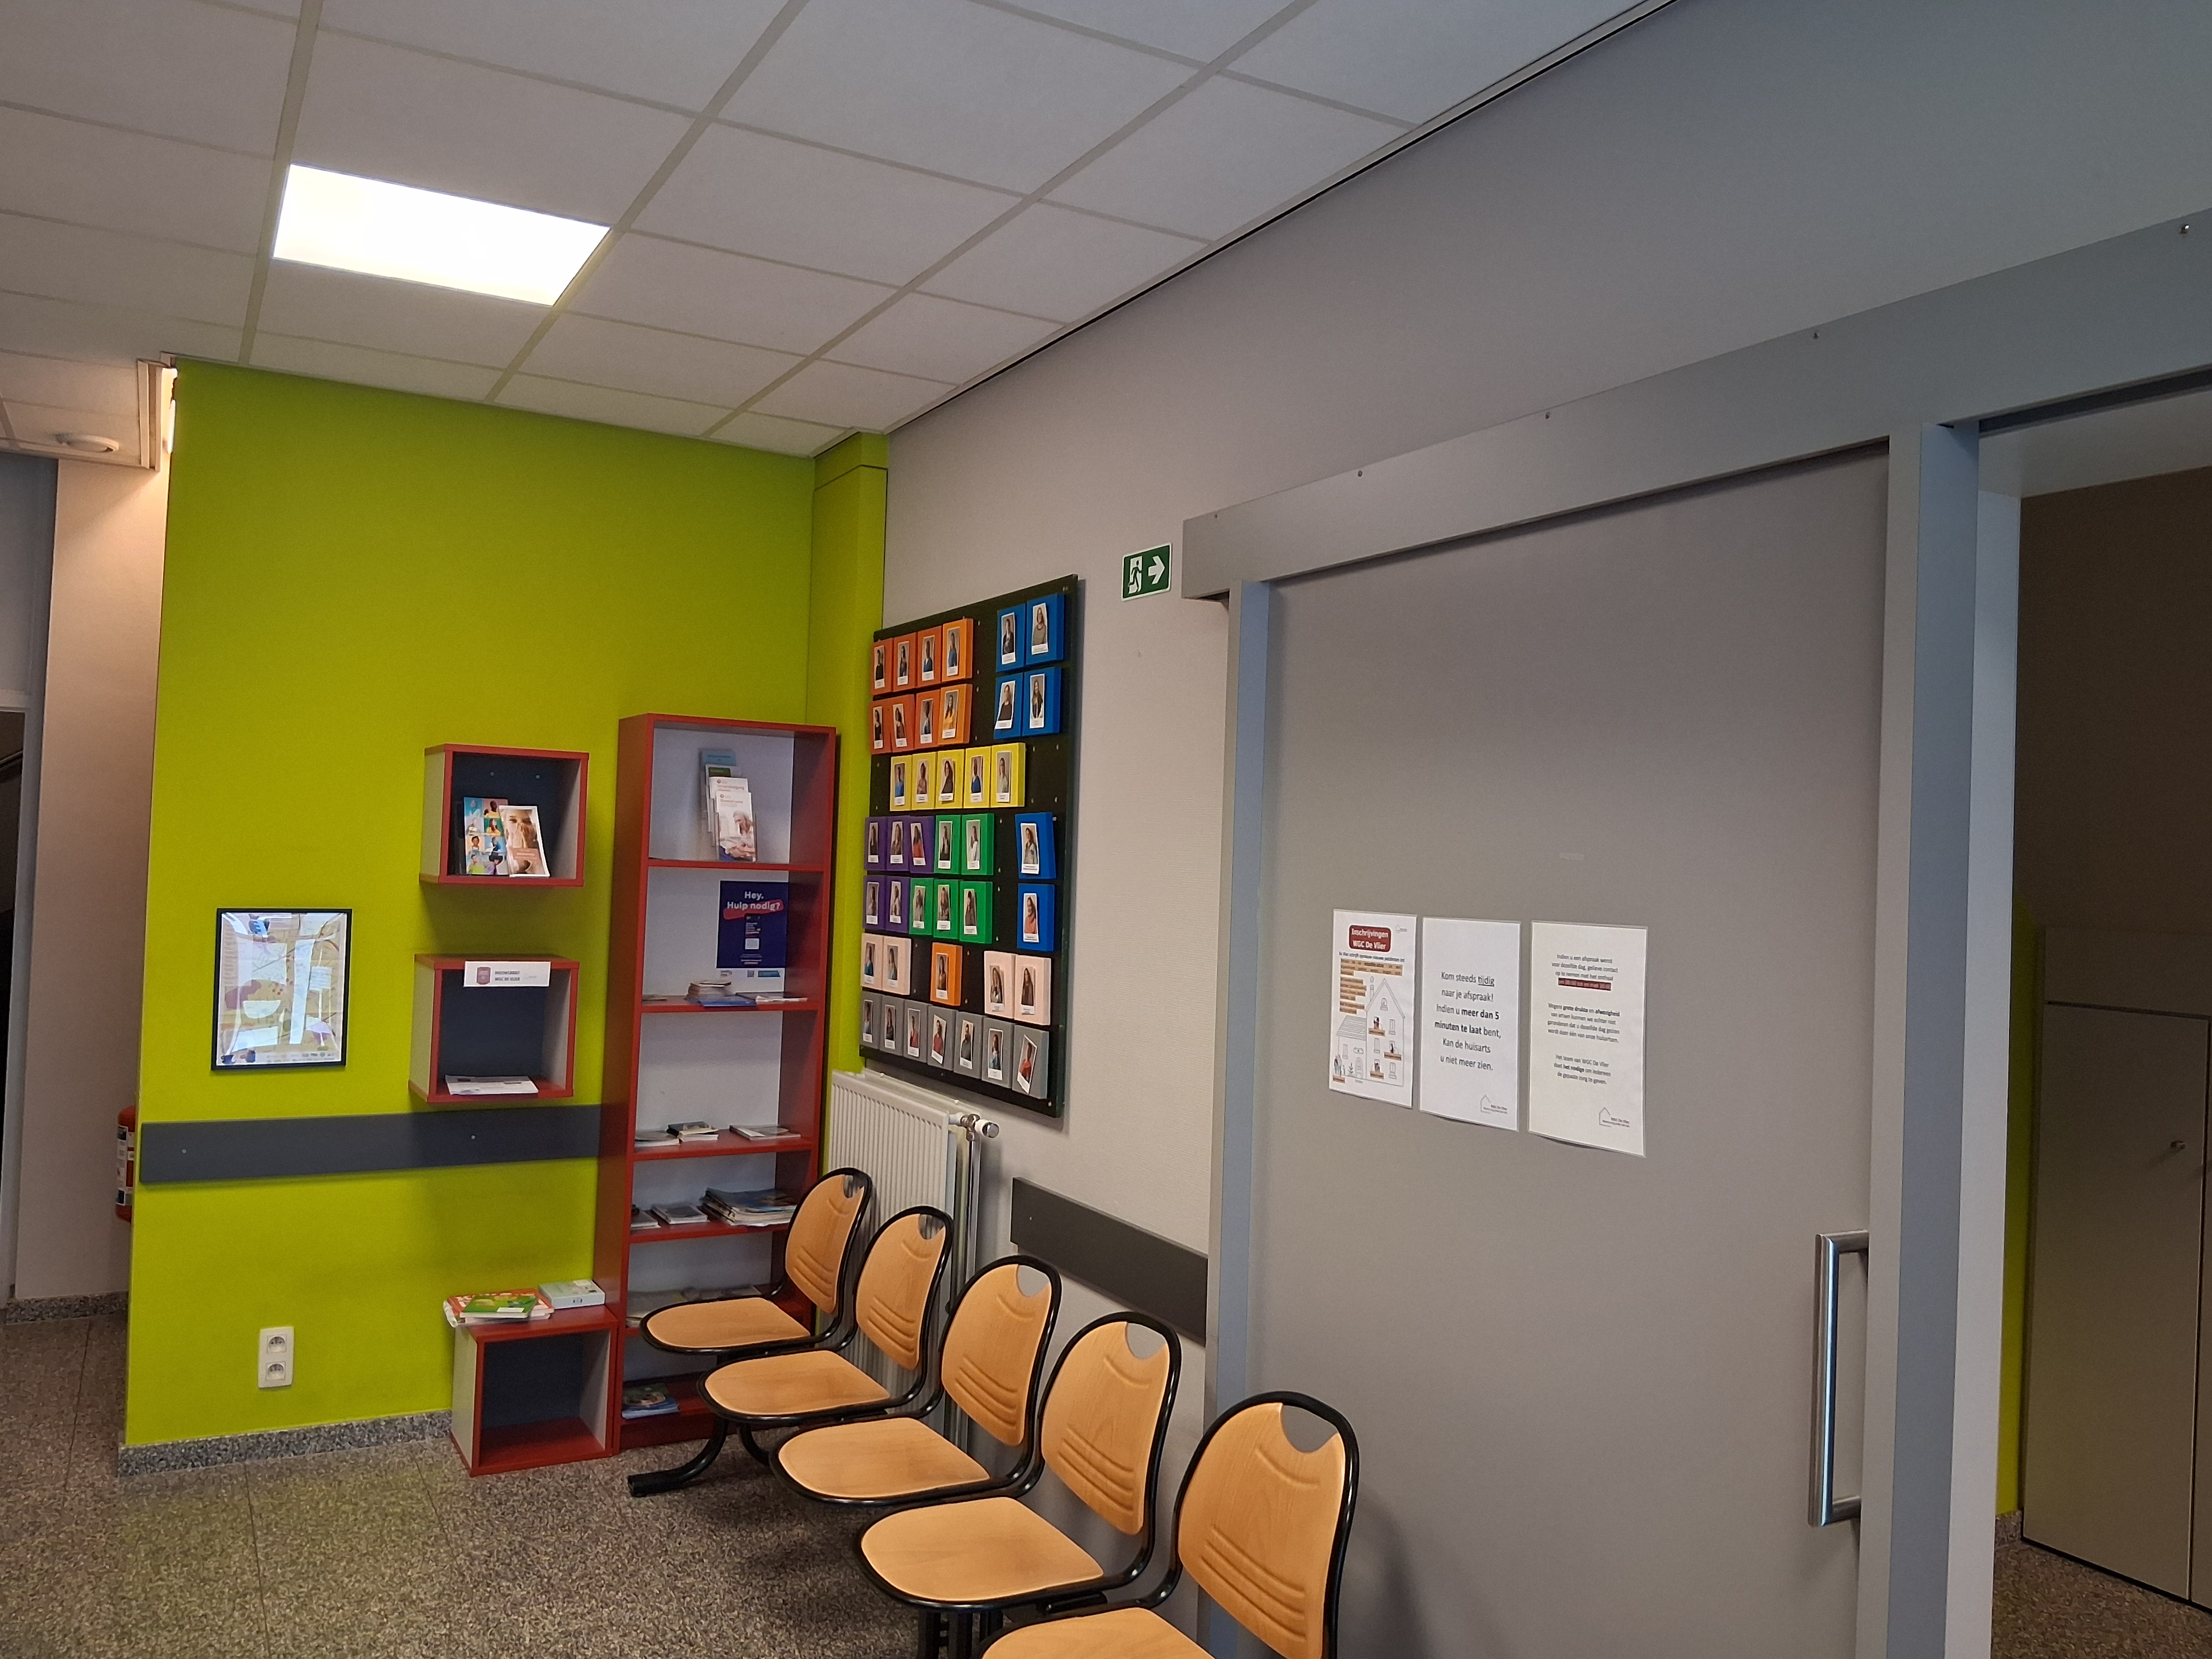
\includegraphics[width=0.46\textwidth]{img/bp/wachtruimtes/wachtruimte3.jpg}
    }
    %\caption{Optioneel bijschrift}
    \label{fig:vier_fotos}
\end{figure}
\clearpage

\appendix
\section*{Bijlage B: Fotodocumentatie van de Test-omgeving}
\addcontentsline{toc}{section}{Bijlage B: Fotodocumentatie van de Test-omgeving}

Hieronder volgt een visueel overzicht van de opstelling van het meetsysteem.

\begin{figure}[h!]
    \centering
    % Eerste foto
    \begin{minipage}{0.48\textwidth}
        \centering
        \rotatebox{270}{%
            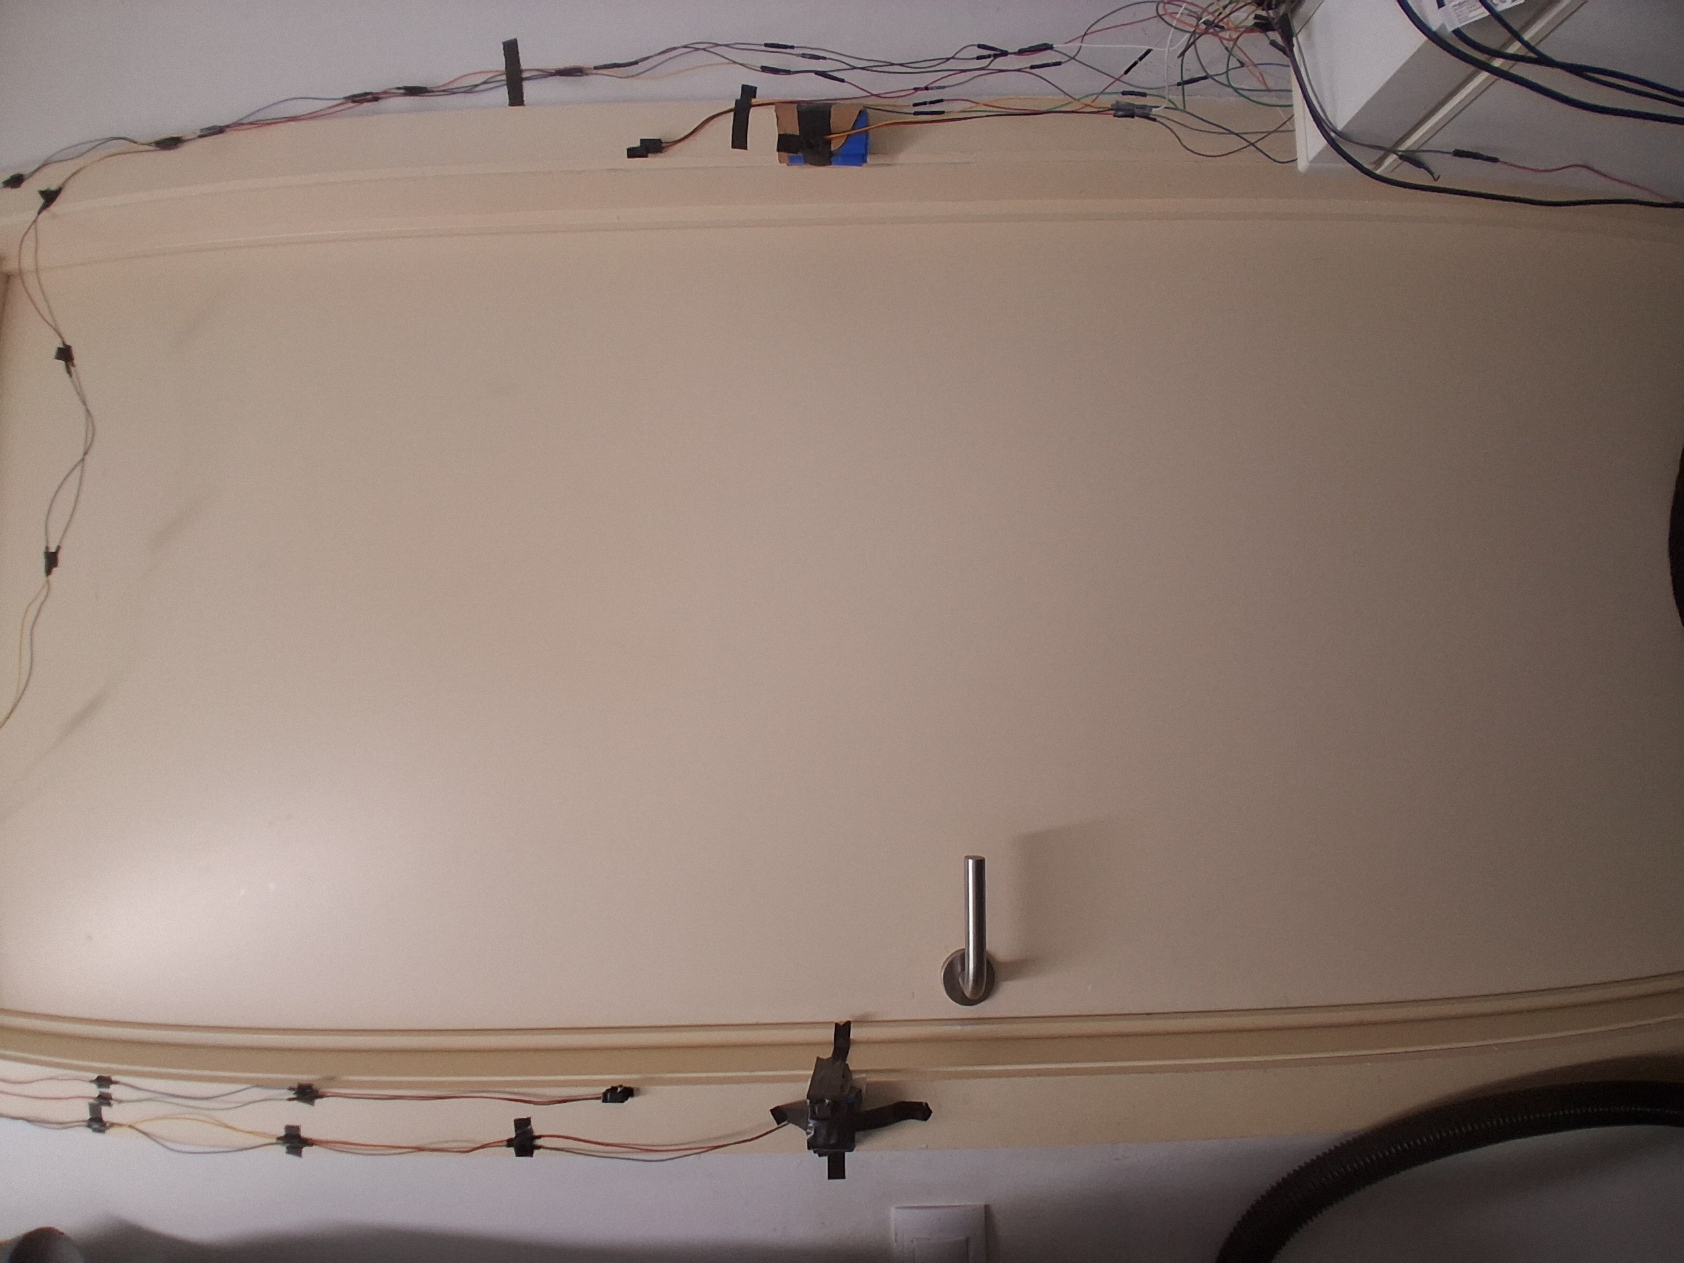
\includegraphics[width=9cm]{img/bp/wachtruimtes/technische_uitwerking/testomgeving.jpg}
        }
        %\caption{Foto 1} % optioneel
    \end{minipage}
    \hspace{0.02\textwidth}
    % Tweede foto
    \begin{minipage}{0.48\textwidth}
        \centering
        \rotatebox{0}{%
            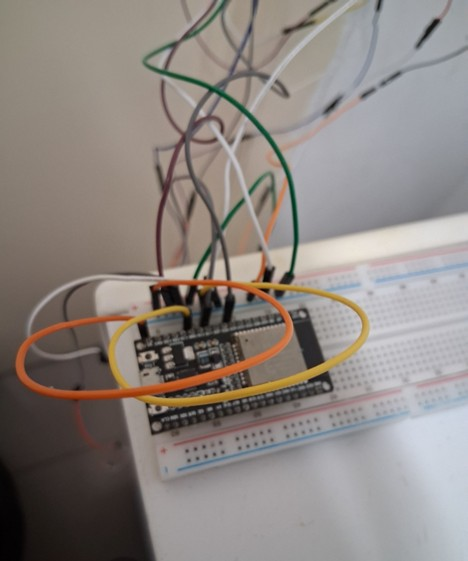
\includegraphics[width=\linewidth]{img/bp/wachtruimtes/technische_uitwerking/testesp.jpg}
        }
        %\caption{Foto 2} % optioneel
    \end{minipage}
    \begin{minipage}{0.48\textwidth}
        \centering
        \rotatebox{270}{%
            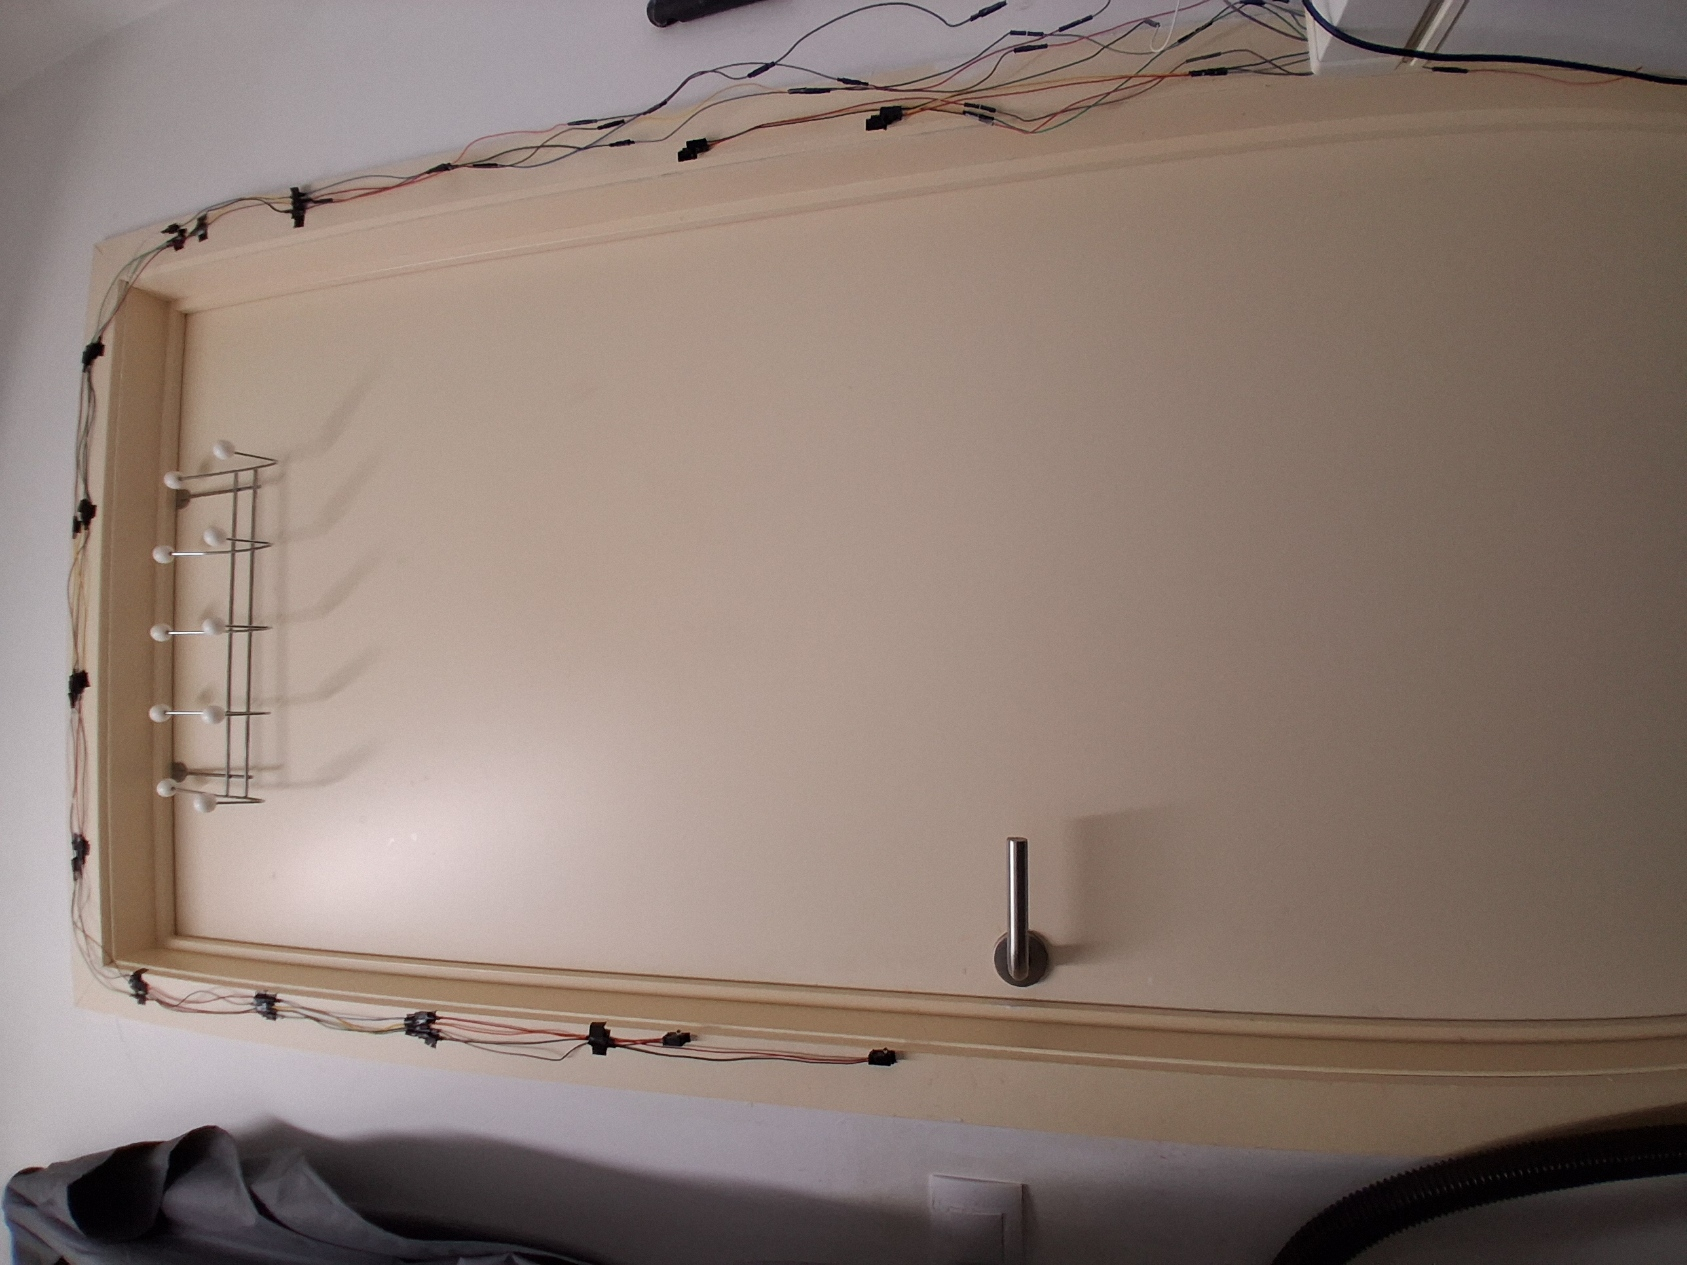
\includegraphics[width=10cm]{img/bp/wachtruimtes/technische_uitwerking/testomgeving1.jpg}
        }
        %\caption{Foto 1} % optioneel
    \end{minipage}
    %\caption{Opstelling van het \gls{iot}-meetsysteem}
    \label{fig:iot_test}
\end{figure}

\clearpage

\appendix
\section*{Bijlage C: Fotodocumentatie van de \gls{iot}-opstelling}
\addcontentsline{toc}{section}{Bijlage C: Fotodocumentatie van de \gls{iot}-opstelling}

Hieronder volgt een visueel overzicht van de opstelling van het meetsysteem.

% Eerste rij van drie foto's (normaal)
\begin{figure}[h!]
    \centering
    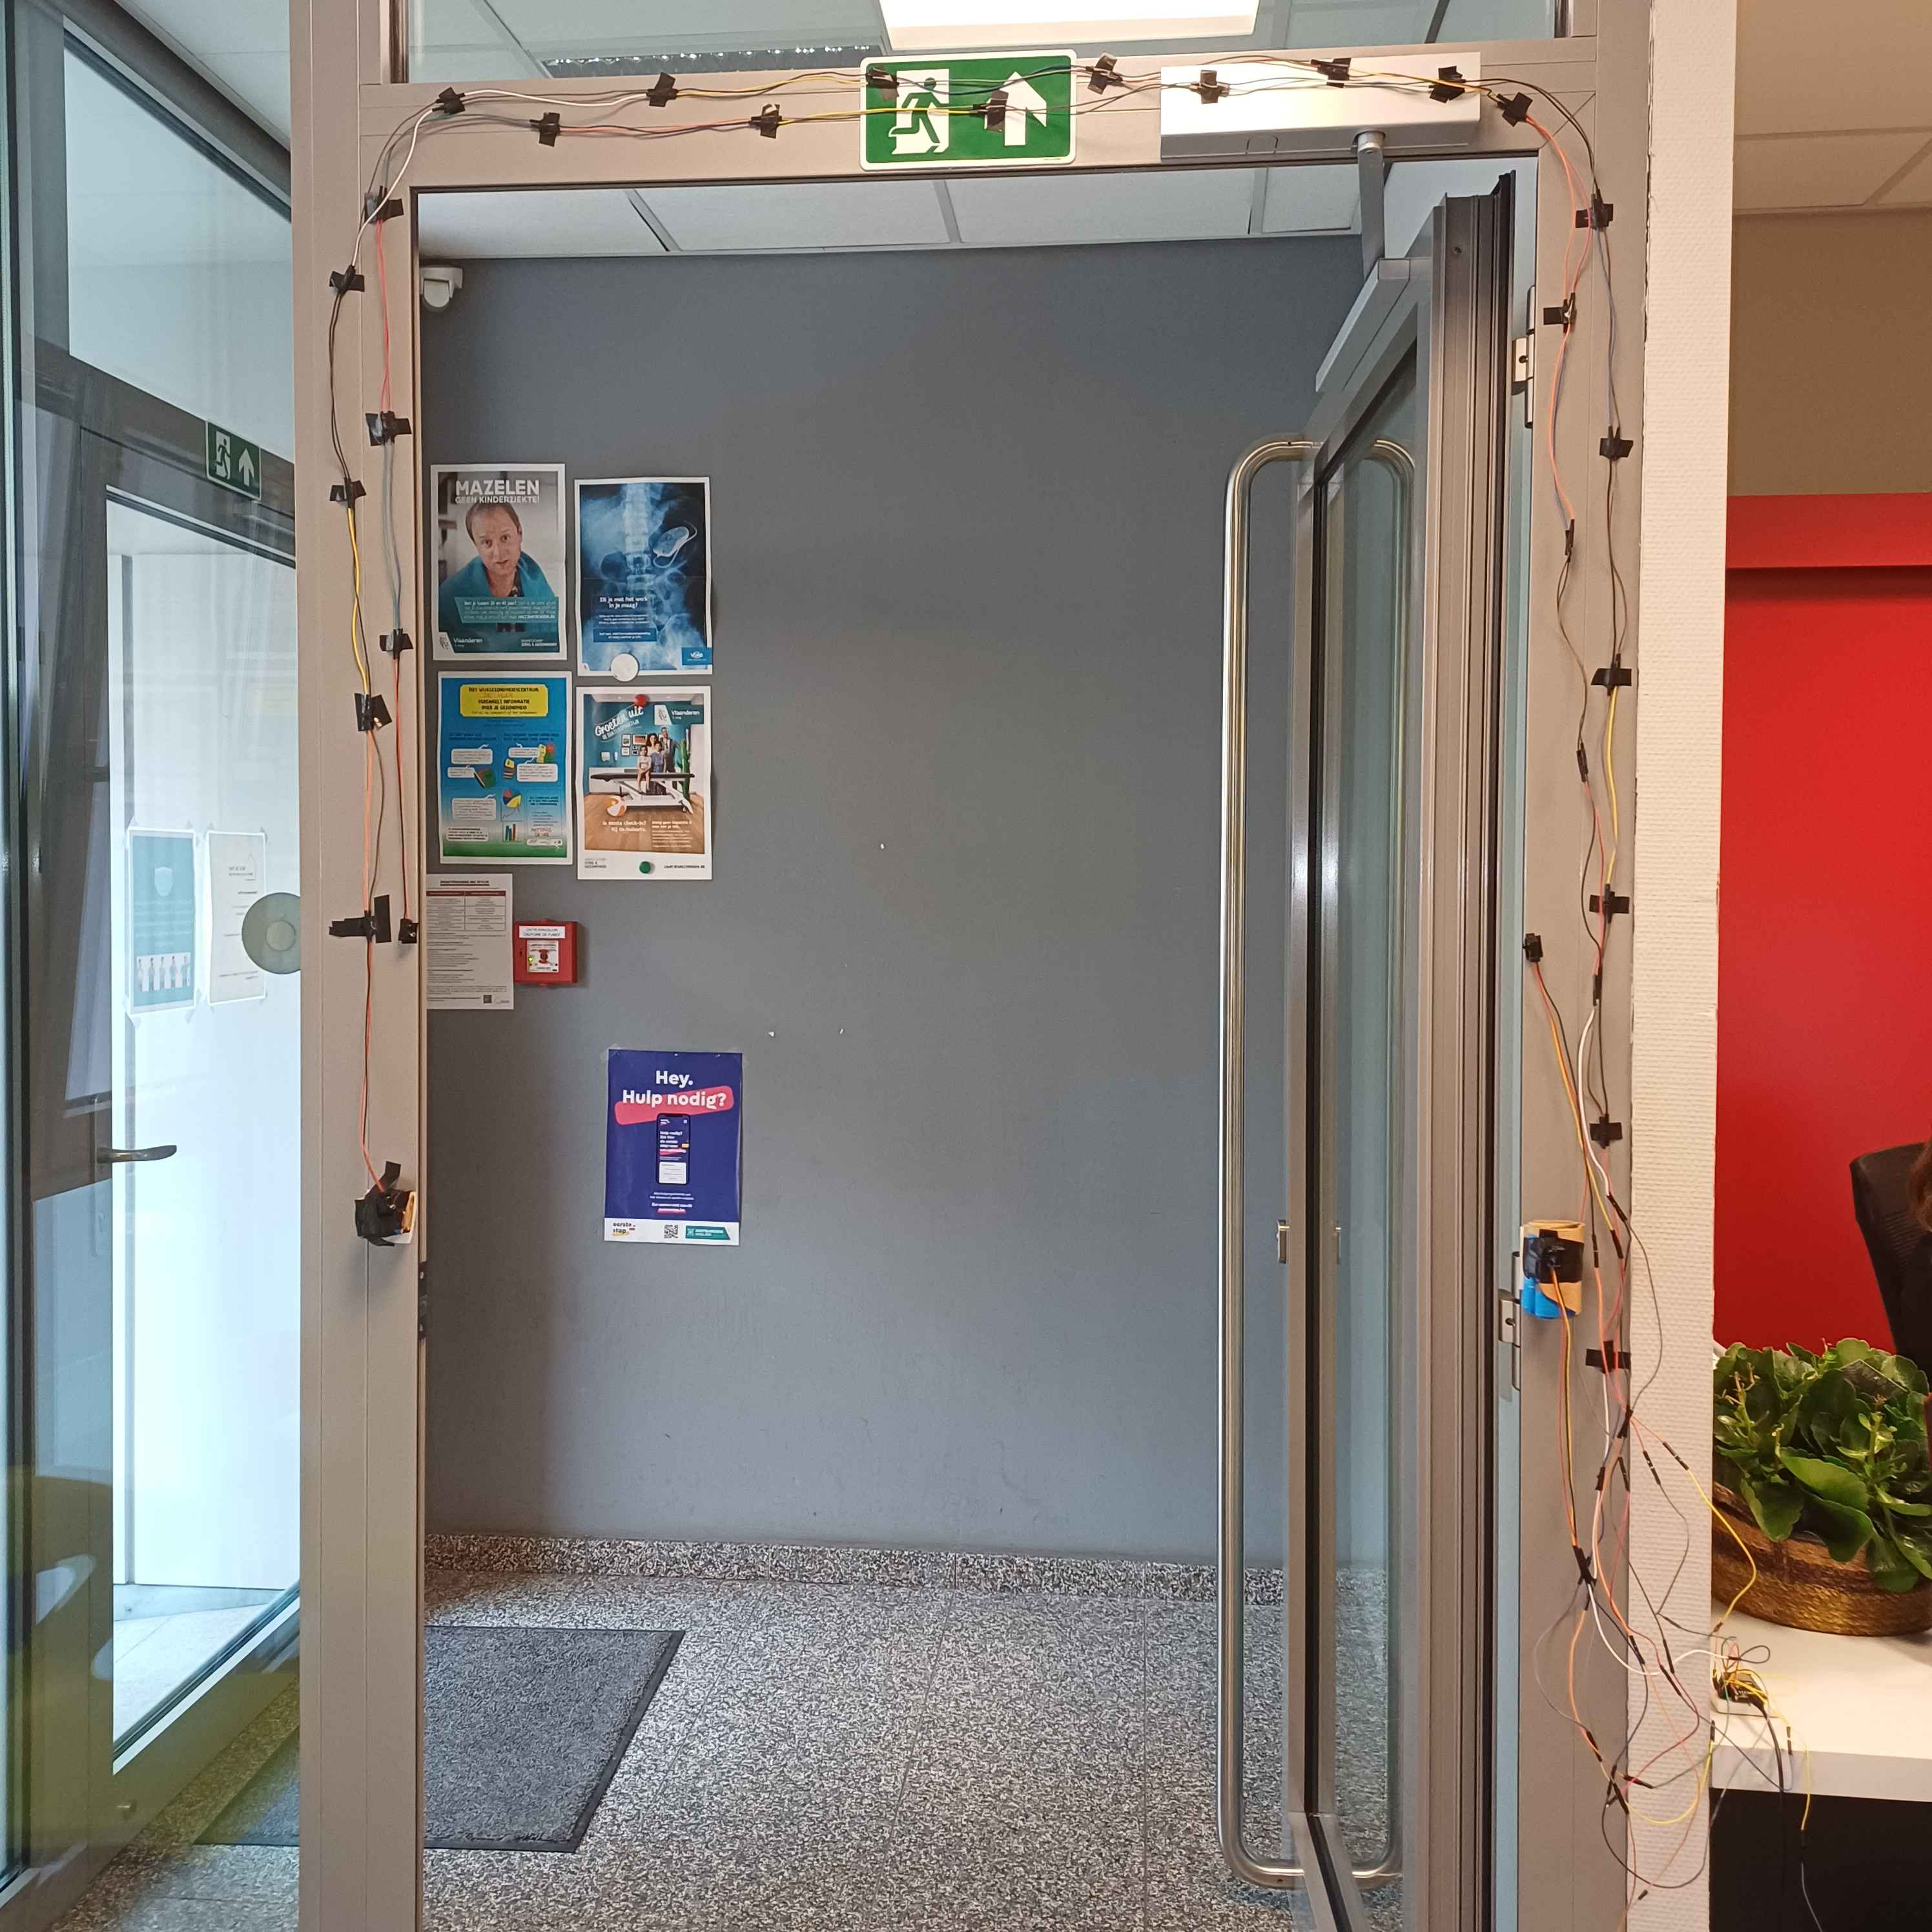
\includegraphics[width=0.55\textwidth]{img/bp/wachtruimtes/technische_uitwerking/door.jpg}
    \hspace{0.02\textwidth}
    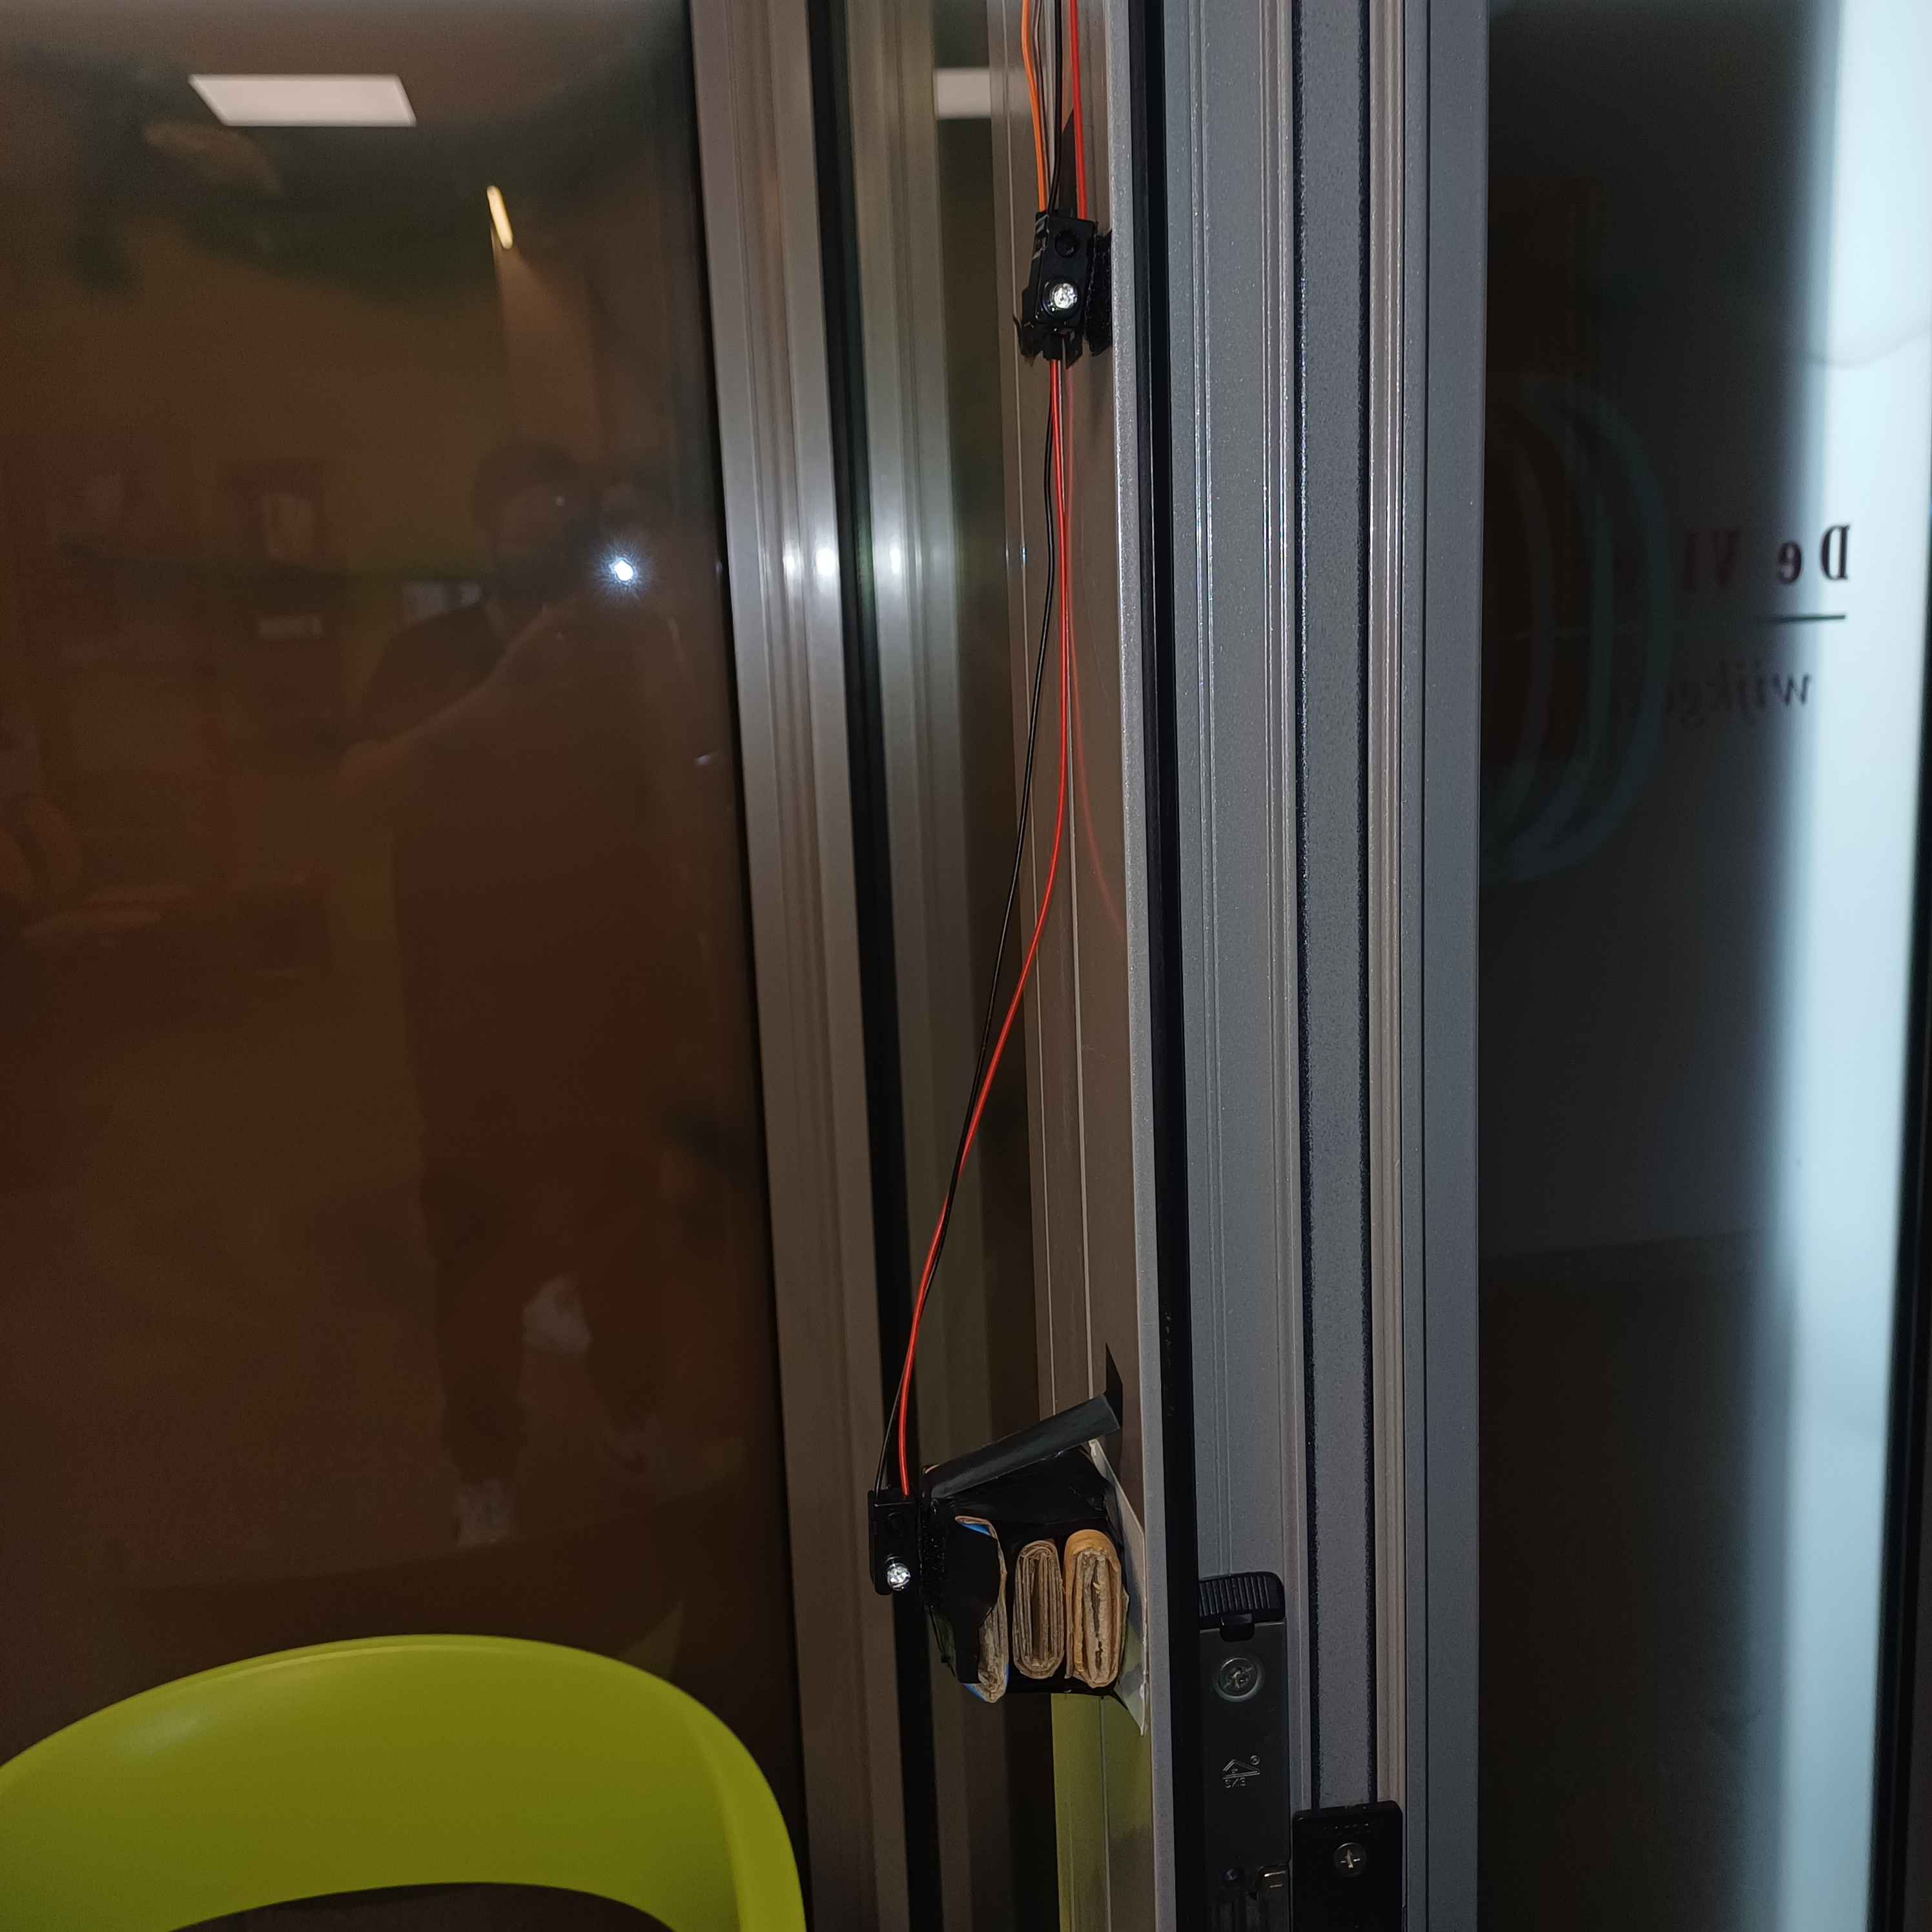
\includegraphics[width=0.48\textwidth]{img/bp/wachtruimtes/technische_uitwerking/emitters.jpg}
    \hspace{0.02\textwidth}
    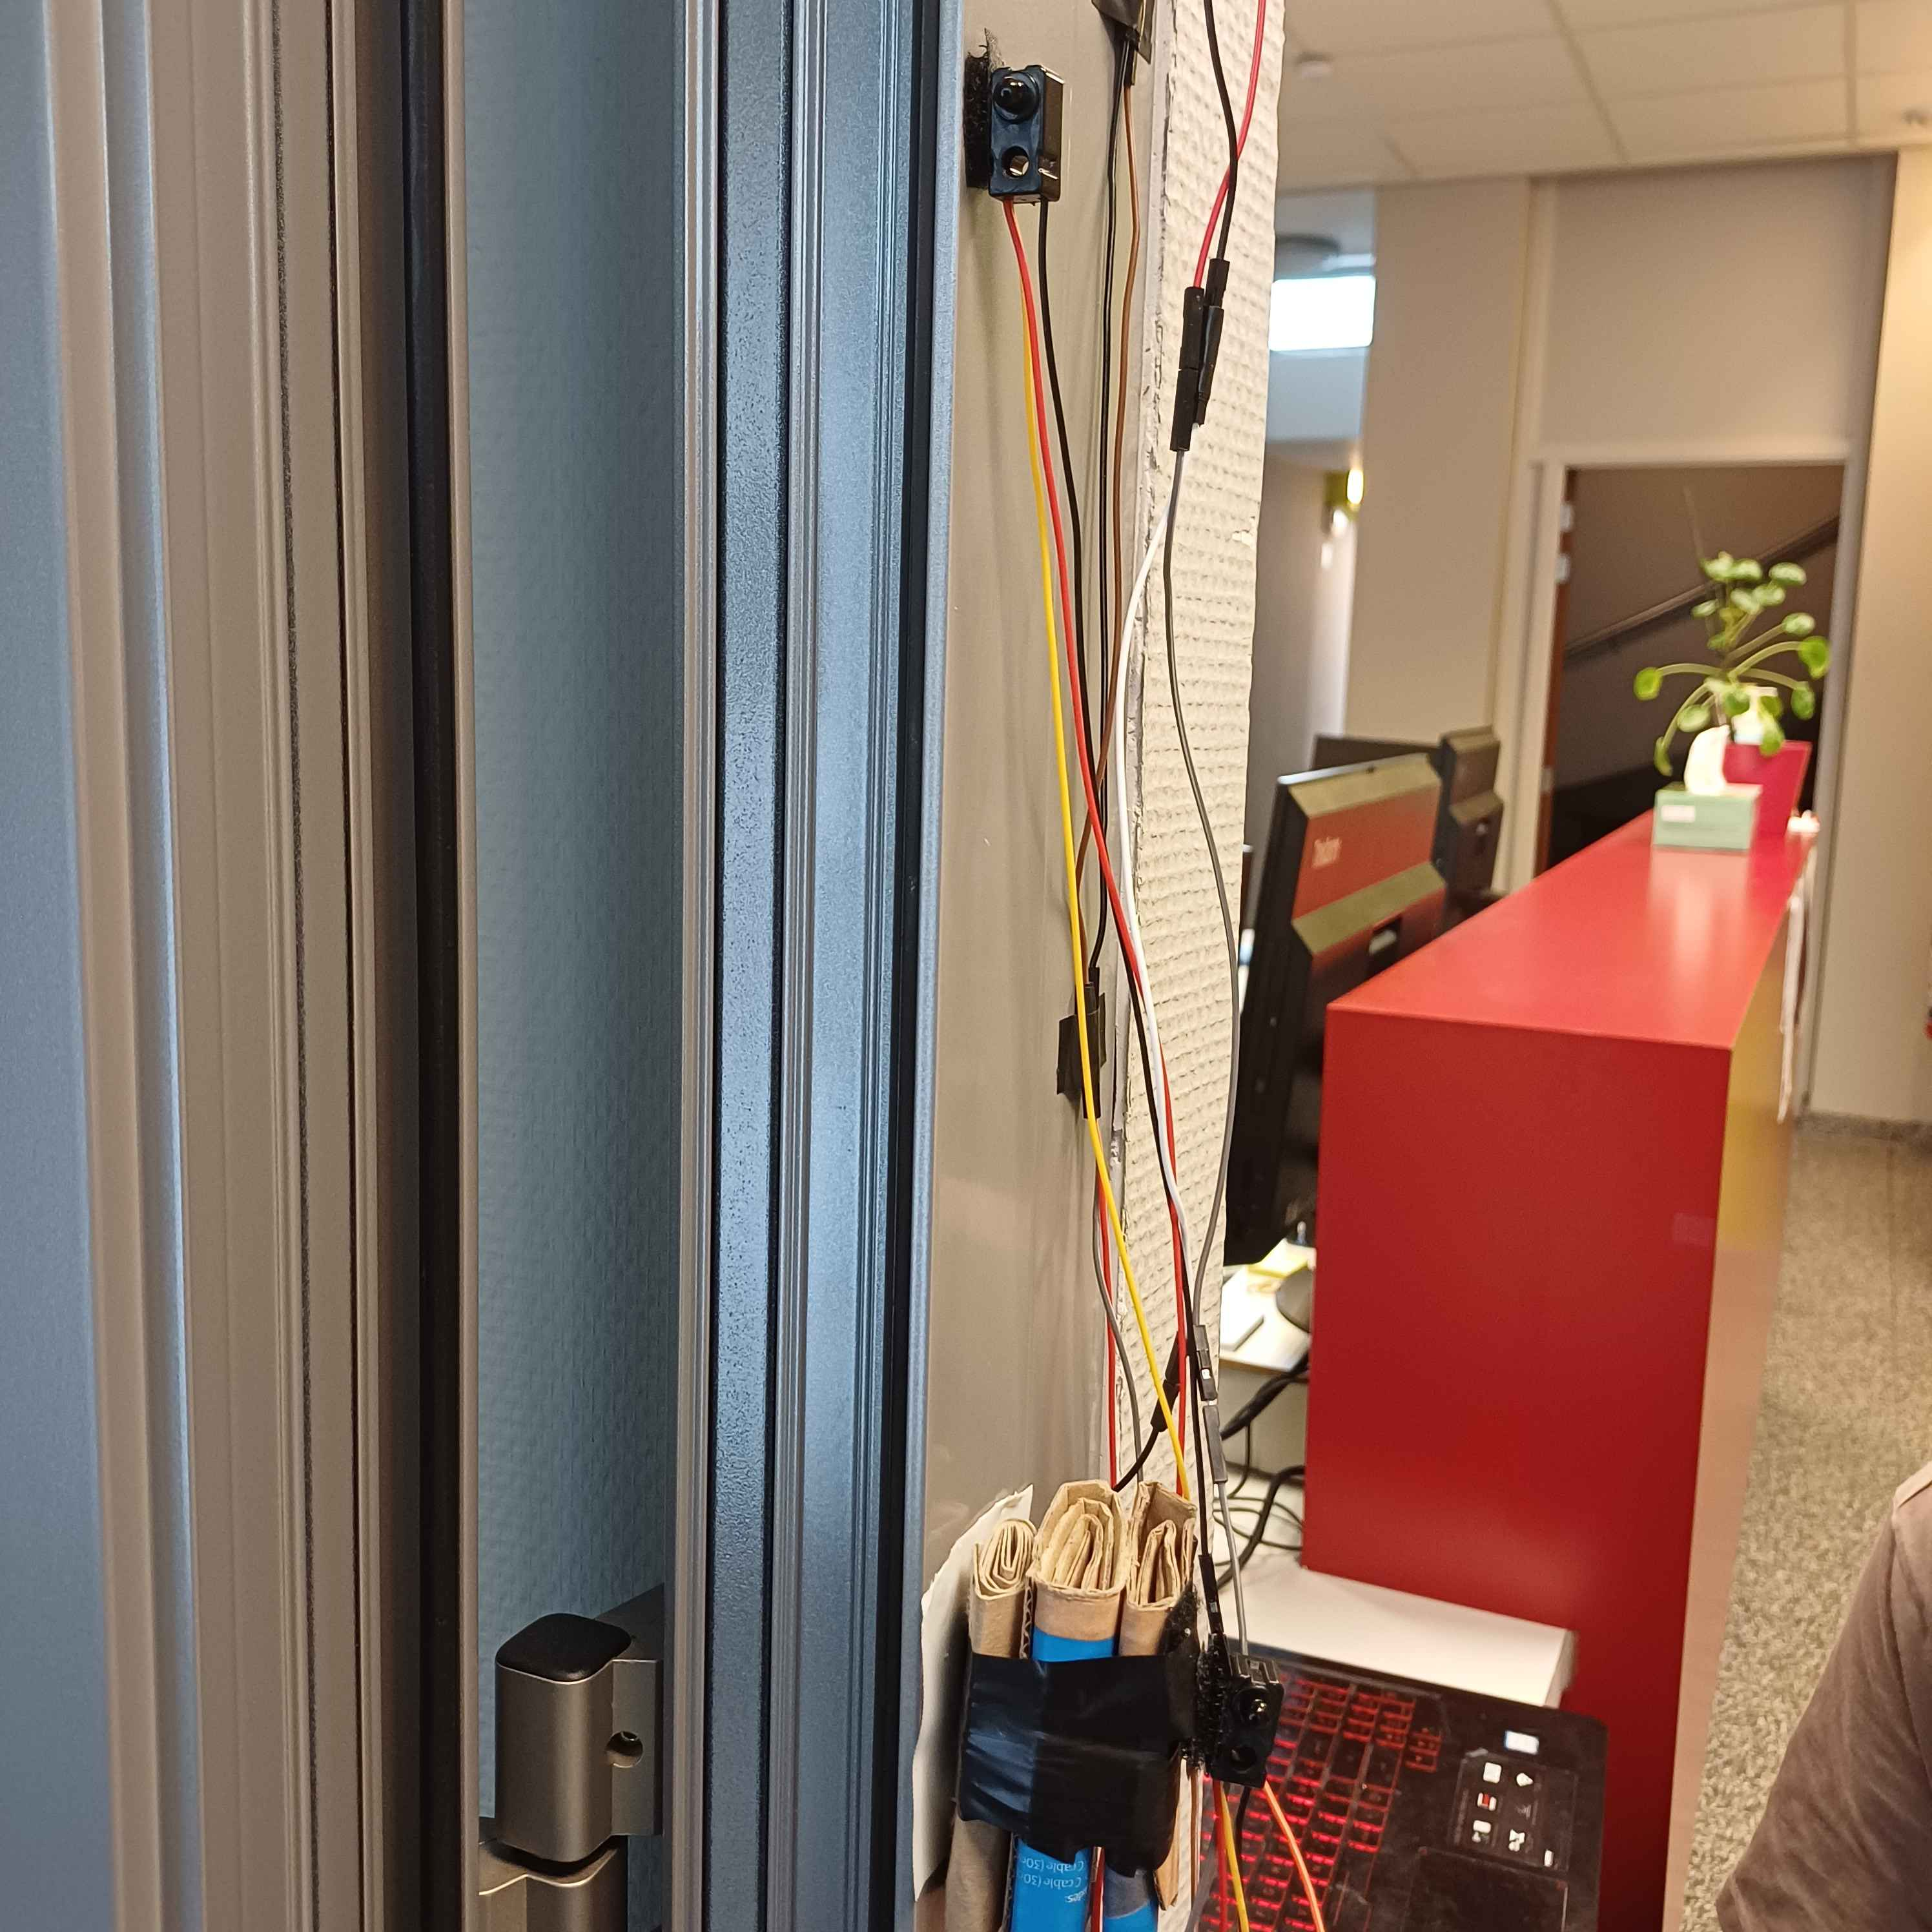
\includegraphics[width=0.48\textwidth]{img/bp/wachtruimtes/technische_uitwerking/receivers.jpg}
    \caption{Bovenste rij: deur, emitters en receivers}
\end{figure}

% Tweede rij van drie foto's (geroteerd)
\begin{figure}[h!]
    \centering
    \rotatebox{270}{\includegraphics[width=0.6\textwidth]{img/bp/wachtruimtes/technische_uitwerking/pi.jpg}}
    \hspace{0.02\textwidth}
    \rotatebox{270}{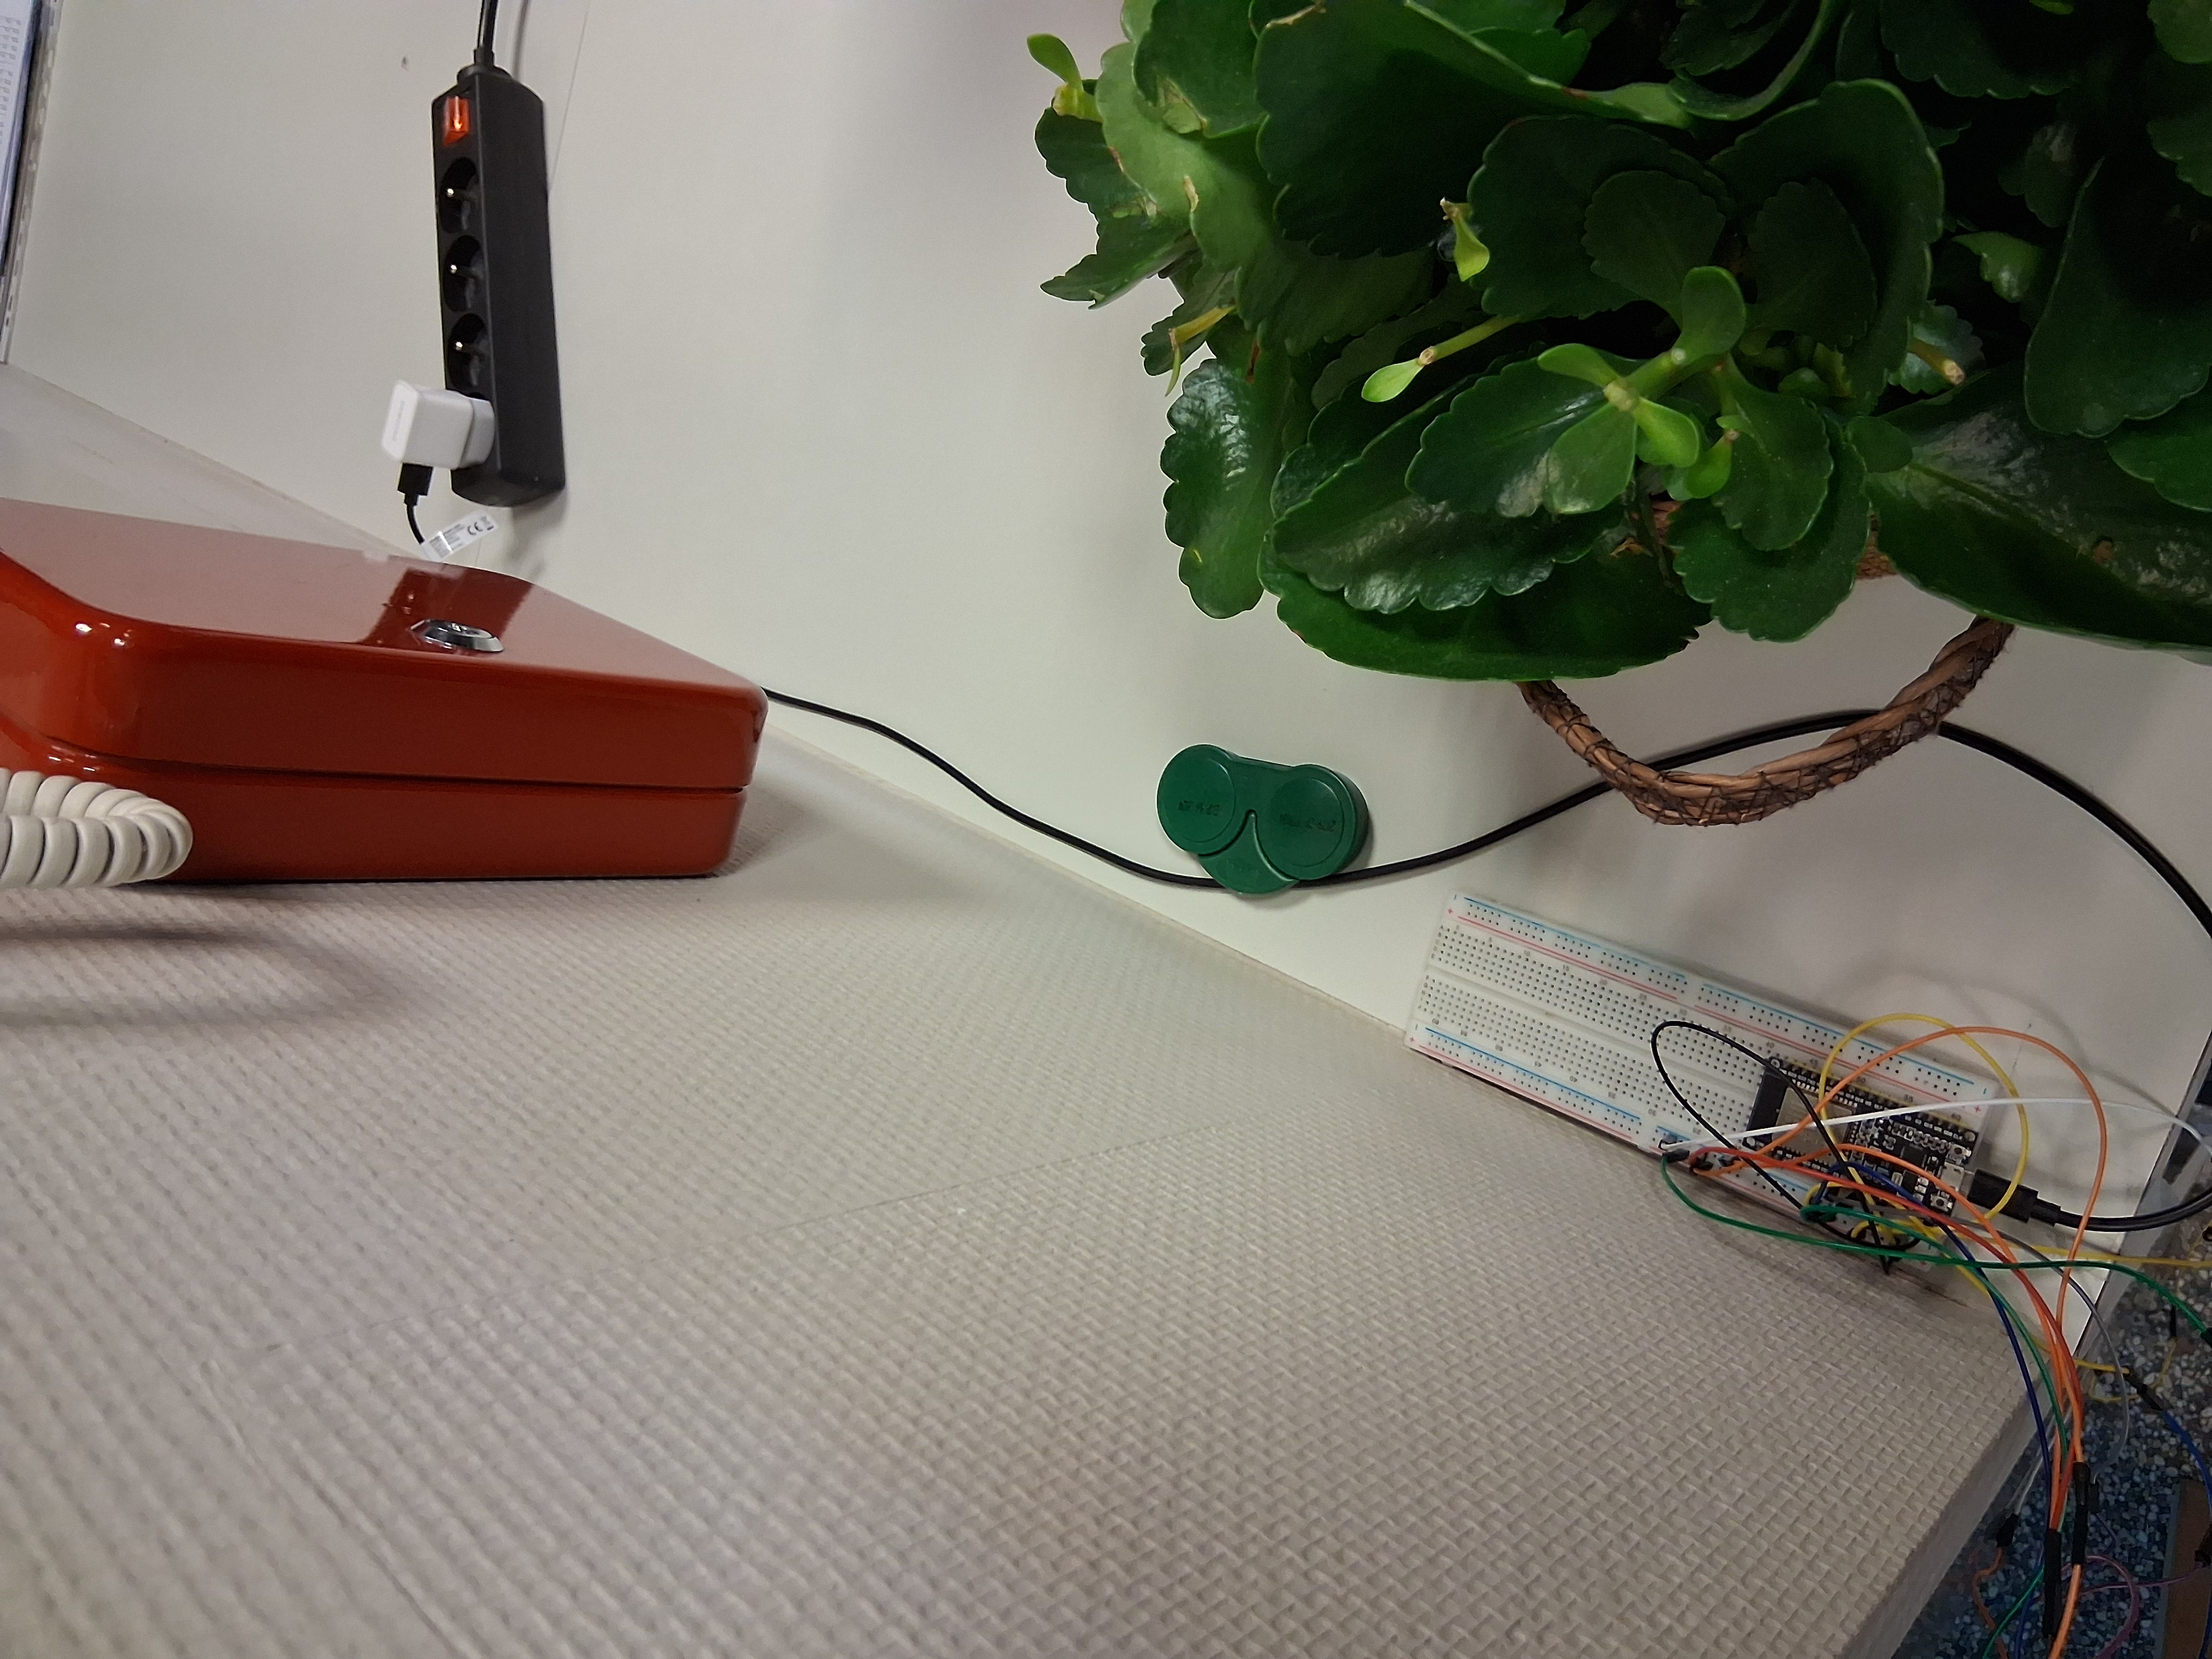
\includegraphics[width=0.6\textwidth]{img/bp/wachtruimtes/technische_uitwerking/esp.jpg}}
    \hspace{0.02\textwidth}
    \rotatebox{270}{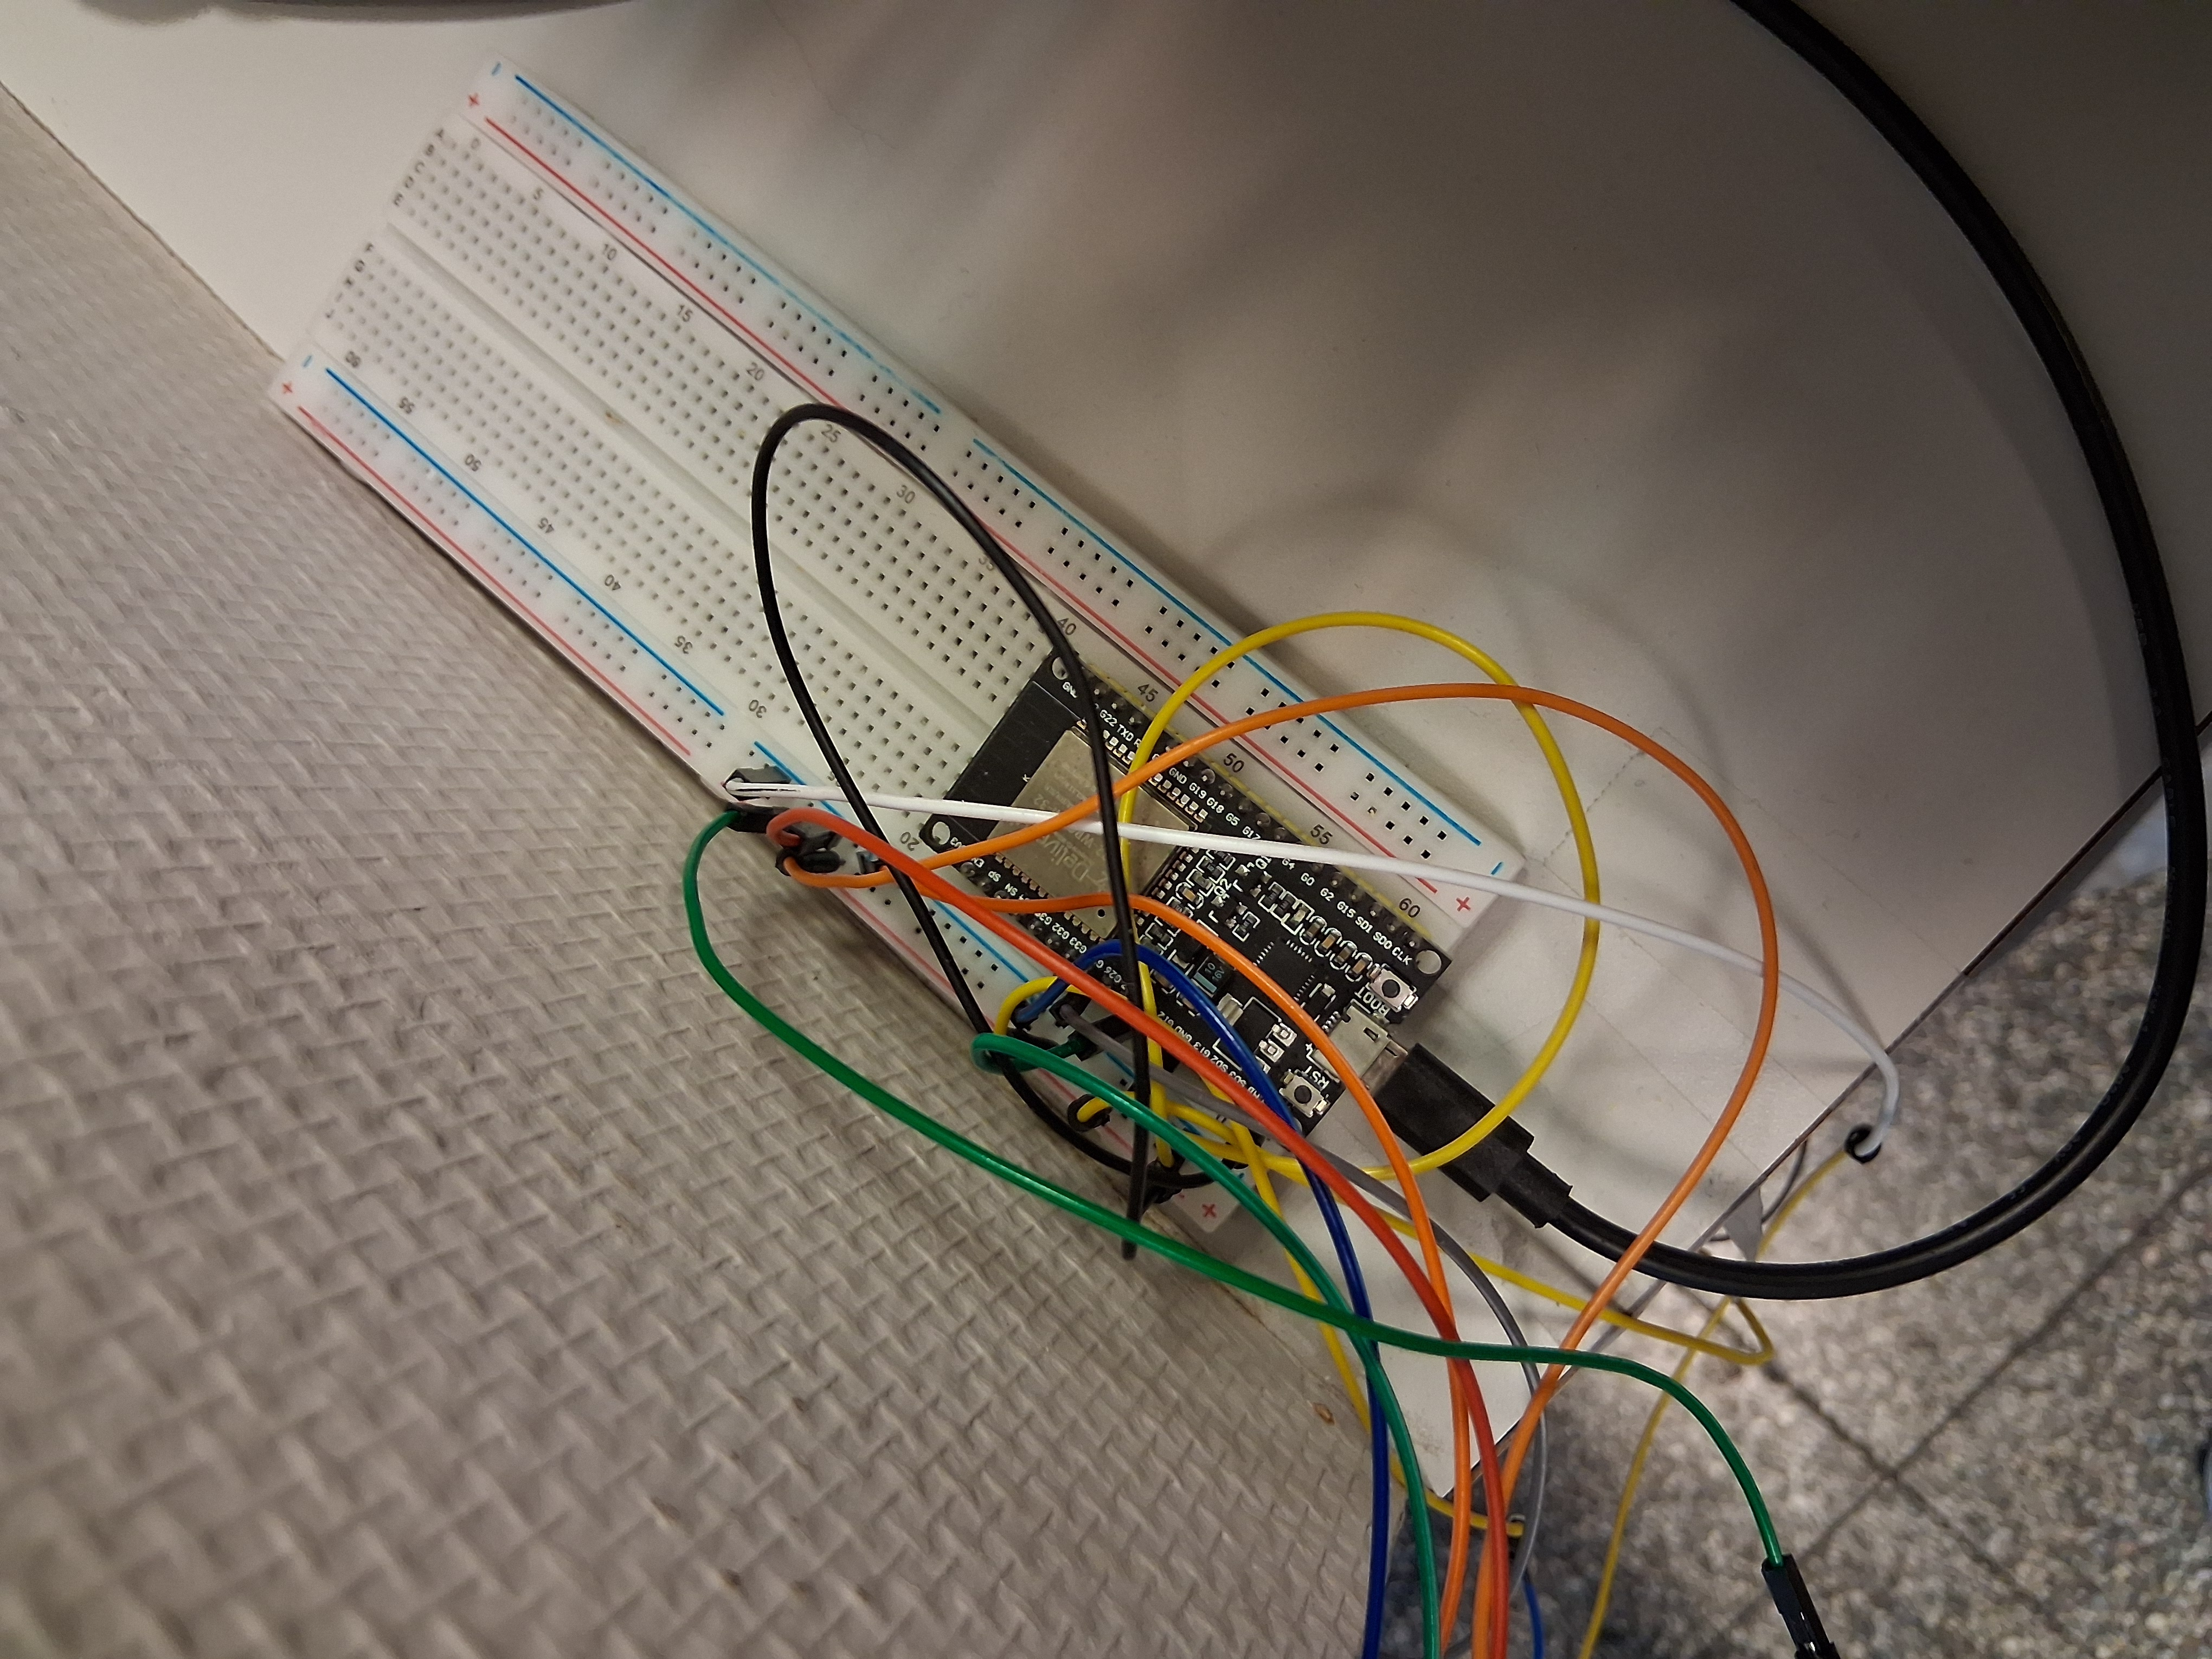
\includegraphics[width=0.6\textwidth]{img/bp/wachtruimtes/technische_uitwerking/esp1.jpg}}
    \caption{Onderste rij: Raspberry Pi en ESP-modules (geroteerd)}
    \label{fig:foto_iot}
\end{figure}








% Voeg hier je eigen hoofdstukken toe die de ``corpus'' van je bachelorproef
% vormen. De structuur en titels hangen af van je eigen onderzoek. Je kan bv.
% elke fase in je onderzoek in een apart hoofdstuk bespreken.

%\input{...}
%\input{...}
%...

%%=============================================================================
%% Conclusie
%%=============================================================================

\chapter{Conclusie}%
\label{ch:conclusie}

% TODO: Trek een duidelijke conclusie, in de vorm van een antwoord op de
% onderzoeksvra(a)g(en). Wat was jouw bijdrage aan het onderzoeksdomein en
% hoe biedt dit meerwaarde aan het vakgebied/doelgroep? 
% Reflecteer kritisch over het resultaat. In Engelse teksten wordt deze sectie
% ``Discussion'' genoemd. Had je deze uitkomst verwacht? Zijn er zaken die nog
% niet duidelijk zijn?
% Heeft het onderzoek geleid tot nieuwe vragen die uitnodigen tot verder 
%onderzoek?

Het centrale onderzoeksvraagstuk in deze bachelorproef is: 
Hoe kan \gls{iot}-technologie worden ingezet om de bezettingsgraad van wachtruimtes in real-time te meten en voorspellende analyses toe te passen, met als doel het inzicht in bezettingsgraden te verbeteren en zo een basis te bieden voor efficiënter bezoekersbeheer? \\

De \gls{poc} toont aan dat \gls{iot}-technologieën in staat zijn om de bezetting in een wachtruimte te detecteren en real-time te registreren. Dit toont de technische haalbaarheid en de potentiële meerwaarde van een sensorgebaseerd systeem.
Bij de samenwerking met \gls{wgc} De Vlier werd het duidelijk dat bezettingsdata gebruikt kan worden als aanvulling voor bestaande data en als ondersteuning kan bieden bij zorgplanning en capaciteitsbeheer. \\

Toch is dit niet genoeg om dit systeem te beschouwen als alternatief door het gebrek aan robuustheid. Storingen en instabiliteit zorgen voor een beperkte dataset waardoor alleen een vergelijking met Vertex AI mogelijk was. Daardoor kon de validatie van de nauwkeurigheid niet worden uitgevoerd. De resultaten tonen dus aan dat de \gls{poc} haalbaar is maar dat de betrouwbaarheid een aandachtspunt blijft. \\

De bijdrage van dit onderzoek ligt in het aantonen dat een \gls{iot}-gebaseerde systeem een privacyvriendelijk en kostenefficiënt alternatief biedt voor vision-gebaseerde oplossingen. Dit kan een meerwaarde bieden voor organisaties (klein tot middengroot) die op zoek zijn naar kostenefficiënte methoden om inzicht te krijgen in wachtruimtebezetting. \\

Voor verdere onderzoek is het essentieel om langere metingen uit te voeren, sensorplaatsing te optimaliseren en stabiliteitsproblemen te reduceren. Dankzij deze aanbevelingen kunnen voorspellende modellen uitgevoerd worden zodat bezettingsanalyse kunnen bijdragen aan efficiënter bezoekers- en personeelsbeheer \\

Samenvattend kan gesteld worden dat het onderzoek gedeeltelijk succesvol was: \gls{iot}-technologie is een veelbelovende basis gebleken voor real-time monitoring, maar verdere stappen zijn nodig om de betrouwbaarheid en praktische inzetbaarheid te garanderen.
%Tegelijkertijd is de robuustheid van het systeem nog onvoldoende om van een volwaardig alternatief te spreken. Storingen in de sensoren en instabiliteit in de dataverzameling leidden tot beperkte datasets, waardoor slechts een kwalitatieve vergelijking met Google Vertex AI Occupancy Analytics mogelijk was. Een sluitende kwantitatieve validatie van de nauwkeurigheid kon daardoor niet worden uitgevoerd. De resultaten moeten dus kritisch worden geïnterpreteerd: de haalbaarheid is aangetoond, maar de betrouwbaarheid blijft een aandachtspunt. \\

%De bijdrage van dit onderzoek ligt in het aantonen dat een \gls{iot}-gebaseerde aanpak een privacyvriendelijk en kostenefficiënt alternatief kan zijn voor vision-gebaseerde oplossingen. Dit biedt meerwaarde voor organisaties die op zoek zijn naar laagdrempelige methoden om inzicht te krijgen in hun wachtruimtebezetting. \\

%Voor toekomstig onderzoek is het essentieel om langere meetcampagnes op te zetten, sensoropstellingen te verfijnen en stabiliteitsproblemen structureel te reduceren. Bovendien is er nood aan het integreren van voorspellende modellen op basis van grotere en consistente datasets, zodat wachttijdanalyses daadwerkelijk kunnen bijdragen aan efficiënter bezoekers- en personeelsbeheer. \\


\printglossaries








%---------- Bijlagen -----------------------------------------------------------

\appendix

\chapter{Onderzoeksvoorstel}

Het onderwerp van deze bachelorproef is gebaseerd op een onderzoeksvoorstel dat vooraf werd beoordeeld door de promotor. Dat voorstel is opgenomen in deze bijlage”.

%% TODO: 
%\section*{Samenvatting}

% Kopieer en plak hier de samenvatting (abstract) van je onderzoeksvoorstel.

% Verwijzing naar het bestand met de inhoud van het onderzoeksvoorstel
%---------- Inleiding ---------------------------------------------------------

% TODO: Is dit voorstel gebaseerd op een paper van Research Methods die je
% vorig jaar hebt ingediend? Heb je daarbij eventueel samengewerkt met een
% andere student?
% Zo ja, haal dan de tekst hieronder uit commentaar en pas aan.

\paragraph{Opmerking}
Dit voorstel is gebaseerd op het onderzoeksvoorstel dat werd geschreven in het
kader van het vak Research Methods dat ik (vorig/dit) academiejaar heb
uitgewerkt (met medestudent Mohammed-Ali Kasraoui als mede-auteur).
 

\section{Inleiding}%
\label{sec:inleiding}

% Waarover zal je bachelorproef gaan? Introduceer het thema en zorg dat volgende zaken zeker duidelijk aanwezig zijn:

%\begin{itemize}
%  \item kaderen thema
%  \item de doelgroep
%  \item de probleemstelling en (centrale) onderzoeksvraag
%  \item de onderzoeksdoelstelling
% \end{itemize}
%
%Denk er aan: een typische bachelorproef is \textit{toegepast onderzoek}, wat betekent dat je start vanuit een concrete probleemsituatie in bedrijfscontext, een \textbf{casus}. Het is belangrijk om je onderwerp goed af te bakenen: je gaat voor die \textit{ene specifieke probleemsituatie} op zoek naar een goede oplossing, op basis van de huidige kennis in het vakgebied.

%De doelgroep moet ook concreet en duidelijk zijn, dus geen algemene of vaag gedefinieerde groepen zoals \emph{bedrijven}, \emph{developers}, \emph{Vlamingen}, enz. Je richt je in elk geval op it-professionals, een bachelorproef is geen populariserende tekst. Eén specifiek bedrijf (die te maken hebben met een concrete probleemsituatie) is dus beter dan \emph{bedrijven} in het algemeen.

%Formuleer duidelijk de onderzoeksvraag! De begeleiders lezen nog steeds te veel voorstellen waarin we geen onderzoeksvraag terugvinden.

%Schrijf ook iets over de doelstelling. Wat zie je als het concrete eindresultaat van je onderzoek, naast de uitgeschreven scriptie? Is het een proof-of-concept, een rapport met aanbevelingen, \ldots Met welk eindresultaat kan je je bachelorproef als een succes beschouwen?

%----------------------------------------------------------Inleiding-------------------------------------------------


De toenemende wachttijden voor behandelingen op de Accident and Emergency (A\&E) afdelingen binnen de National Health Service (NHS) \ref{fig:Figuur0} vormen een groeiend probleem in het Verenigd Koninkrijk en zijn daarom de oorzaak van veel discussie in de Britse media. Dit werd verder versterkt dankzij een recent onderzoek uitgevoerd door The Rt Hon. Professor the Lord Darzi of Denham, een lid van de House of Lords van het Verenigd Koninkrijk.

\subsubsection*{Probleemstelling}
Volgens de bevindingen uit het onderzoek zitten de A\&E afdelingen van de NHS in een “vreselijke staat”. De studie toont namelijk aan dat meer dan 100.000 kinderen vorig jaar meer dan 6 uur moesten wachten en dat bijna 10 procent van alle patiënten nu 12 uur of langer moet wachten om behandeld te worden \autocite{LordDarzi2024}. Deze langdurige wachttijden hebben serieuze consequenties voor patiënten. Volgens een toespraak over het onderzoek door de Britse Premier, Sir Keir Starmer, zijn de lange A\&E wachttijden niet alleen een bron van angst en bezorgdheid, maar leiden ook tot duizenden vermijdbare sterfgevallen. Volgens de Royal College of Emergency Medicine gaat het om 14.000 extra sterfgevallen per jaar \autocite{Starmer2024}.

\subsubsection*{Doel van het Onderzoek}
Om een oplossing te vinden voor dit langdurige probleem richt dit onderzoek zich op het uitzoeken of Internet of Things (IoT) een daadwerkelijke oplossing kan zijn om de lange wachttijden op de Accident and Emergency (A\&E) afdelingen in Engeland te verkorten. Deze studie zal verkennen wat de oorzaak is van de lange wachttijden door een oorzaakanalyse uit te voeren en gegevens te verzamelen van meerdere National Health Service ziekenhuizen. 

\subsubsection*{Onderzoeksvraag}
De centrale onderzoeksvraag in dit onderzoek luidt: "Kunnen Internet of Things (IoT)-technologieën worden toegepast om wachttijden op de Accident and Emergency (A\&E) te verminderen en de efficiëntie van de zorgverlening te verbeteren binnen de National Health Service (NHS)?" Om deze vraag te beantwoorden is het ook van uiterst belang om een antwoord te geven op een aantal deelvragen. Ten eerste: Wat is de oorzaak van de lange Accident and Emergency (A\&E).  Dit is een belangrijke vraag om te bepalen of IoT een geschikte oplossing kan zijn bij het verkorten van de wachttijden. Ten tweede: Welke IoT devices kunnen ingezet worden om de oorzaak te verhelpen. Ten laatste: hoe kan er juist bewezen worden dat IoT de wachttijd kan verkorten? Na beantwoorden van deze onderzoeksvragen kunnen er diverse conclusies getrokken worden met betrekking tot IoT en de lange Accident and Emergency (A\&E) wachttijden.


\subsubsection*{Onderzoeksdoelstelling}
Het is van cruciaal belang om dit onderwerp te onderzoeken vanwege de potentiële impact op de gezondheidszorg en het welzijn van patiënten binnen de NHS. De onderzoeksdoelstelling is om te bepalen of IoT een werkelijke oplossing kan bieden voor de lange A\&E wachttijden.

\subsubsection*{Verwacht Eindresultaat}
Het concrete eindresultaat van dit onderzoek zal zijn om aanbevelingen te formuleren voor de implementatie van Internet of Things (IoT)-oplossingen binnen de Accident and Emergency (A\&E)-afdelingen van NHS-ziekenhuizen, met als doel de wachttijden te verminderen en de kwaliteit van zorg te verbeteren.

\begin{figure}[h]
    \centering
    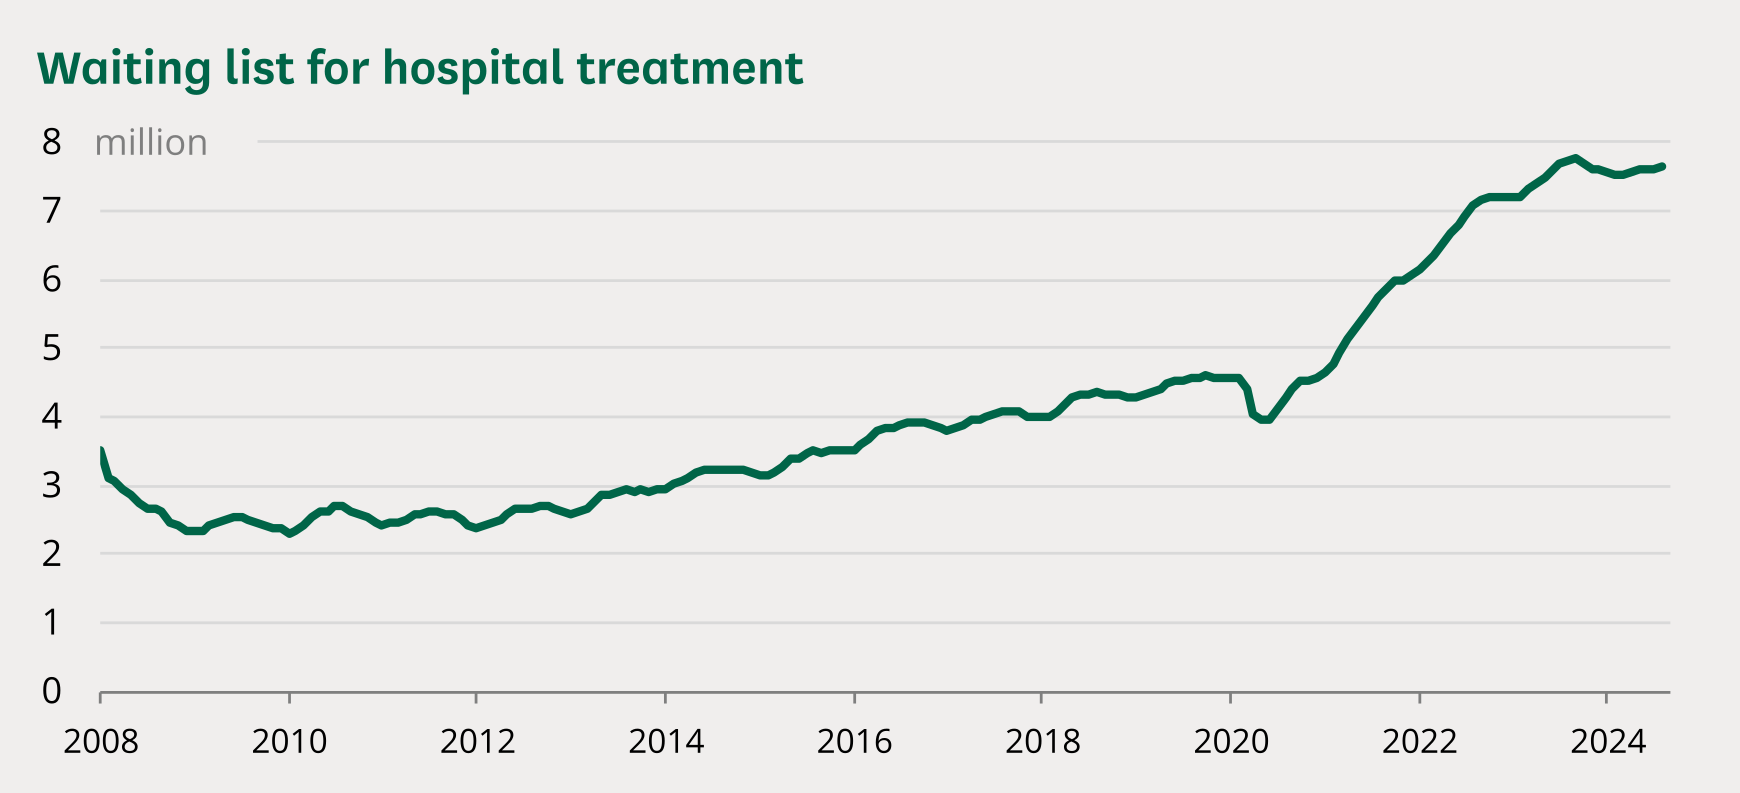
\includegraphics[width=1\linewidth]{img/Figuur-0.png}
    \caption{Wachtlijst van miljoenen patiënten voor ziekenhuisbehandeling (2011 - 2024)}
    \label{fig:Figuur0}
    \textit{Source: \autocite{Stiebahl2024}}
\end{figure}


%---------- Stand van zaken ---------------------------------------------------

\section{Literatuurstudie}%
\label{sec:literatuurstudie}

%Hier beschrijf je de \emph{state-of-the-art} rondom je gekozen onderzoeksdomein, d.w.z.\ een inleidende, doorlopende tekst over het onderzoeksdomein van je bachelorproef. Je steunt daarbij heel sterk op de professionele \emph{vakliteratuur}, en niet zozeer op populariserende teksten voor een breed publiek. Wat is de huidige stand van zaken in dit domein, en wat zijn nog eventuele open vragen (die misschien de aanleiding waren tot je onderzoeksvraag!)?

%Je mag de titel van deze sectie ook aanpassen (literatuurstudie, stand van zaken, enz.). Zijn er al gelijkaardige onderzoeken gevoerd? Wat concluderen ze? Wat is het verschil met jouw onderzoek?

% Verwijs bij elke introductie van een term of bewering over het domein naar de vakliteratuur, bijvoorbeeld~\autocite{Hykes2013}! Denk zeker goed na welke werken je refereert en waarom.

%Draag zorg voor correcte literatuurverwijzingen! Een bronvermelding hoort thuis \emph{binnen} de zin waar je je op die bron baseert, dus niet er buiten! Maak meteen een verwijzing als je gebruik maakt van een bron. Doe dit dus \emph{niet} aan het einde van een lange paragraaf. Baseer nooit teveel aansluitende tekst op eenzelfde bron.

%Als je informatie over bronnen verzamelt in JabRef, zorg er dan voor dat alle nodige info aanwezig is om de bron terug te vinden (zoals uitvoerig besproken in de lessen Research Methods).

% Voor literatuurverwijzingen zijn er twee belangrijke commando's:
% \autocite{KEY} => (Auteur, jaartal) Gebruik dit als de naam van de auteur
%   geen onderdeel is van de zin.
% \textcite{KEY} => Auteur (jaartal)  Gebruik dit als de auteursnaam wel een
%   functie heeft in de zin (bv. ``Uit onderzoek door Doll & Hill (1954) bleek
%   ...'')

%Je mag deze sectie nog verder onderverdelen in subsecties als dit de structuur van de tekst kan verduidelijken.


In de laatste decennia zijn de wachttijden voor de Accident and Emergency (A\&E) afdelingen binnen de National Health Service (NHS) substantieel toegenomen gekend zoals aangetoond in fig. \ref{fig:Figuur1}. Een recente onderzoeksbriefing uitgevoerd door \autocite{Baker2024} toont een sterke toename in de verhouding van patiënten die meer dan vier uur spenderen in de Accident and Emergency (A\&E) afdeling, en dit tussen 2015 en 2020. Sindsdien is er een nieuw record bereikt met 50,4\% van patiënten die meer dan vier uur doorbrengen in de Accident and Emergency (A\&E) afdeling. Dit vormt een duidelijke ondermijning van de vieruursnorm geïmplementeerd door de National Health Service (NHS). Deze richtlijn houdt in dat tenminste 95\% van de patiënten binnen vier uur moeten worden opgenomen, overgebracht en ontslagen worden. \autocite{NationalStatisticsONS2024}.

\begin{figure}[h]
    \centering
    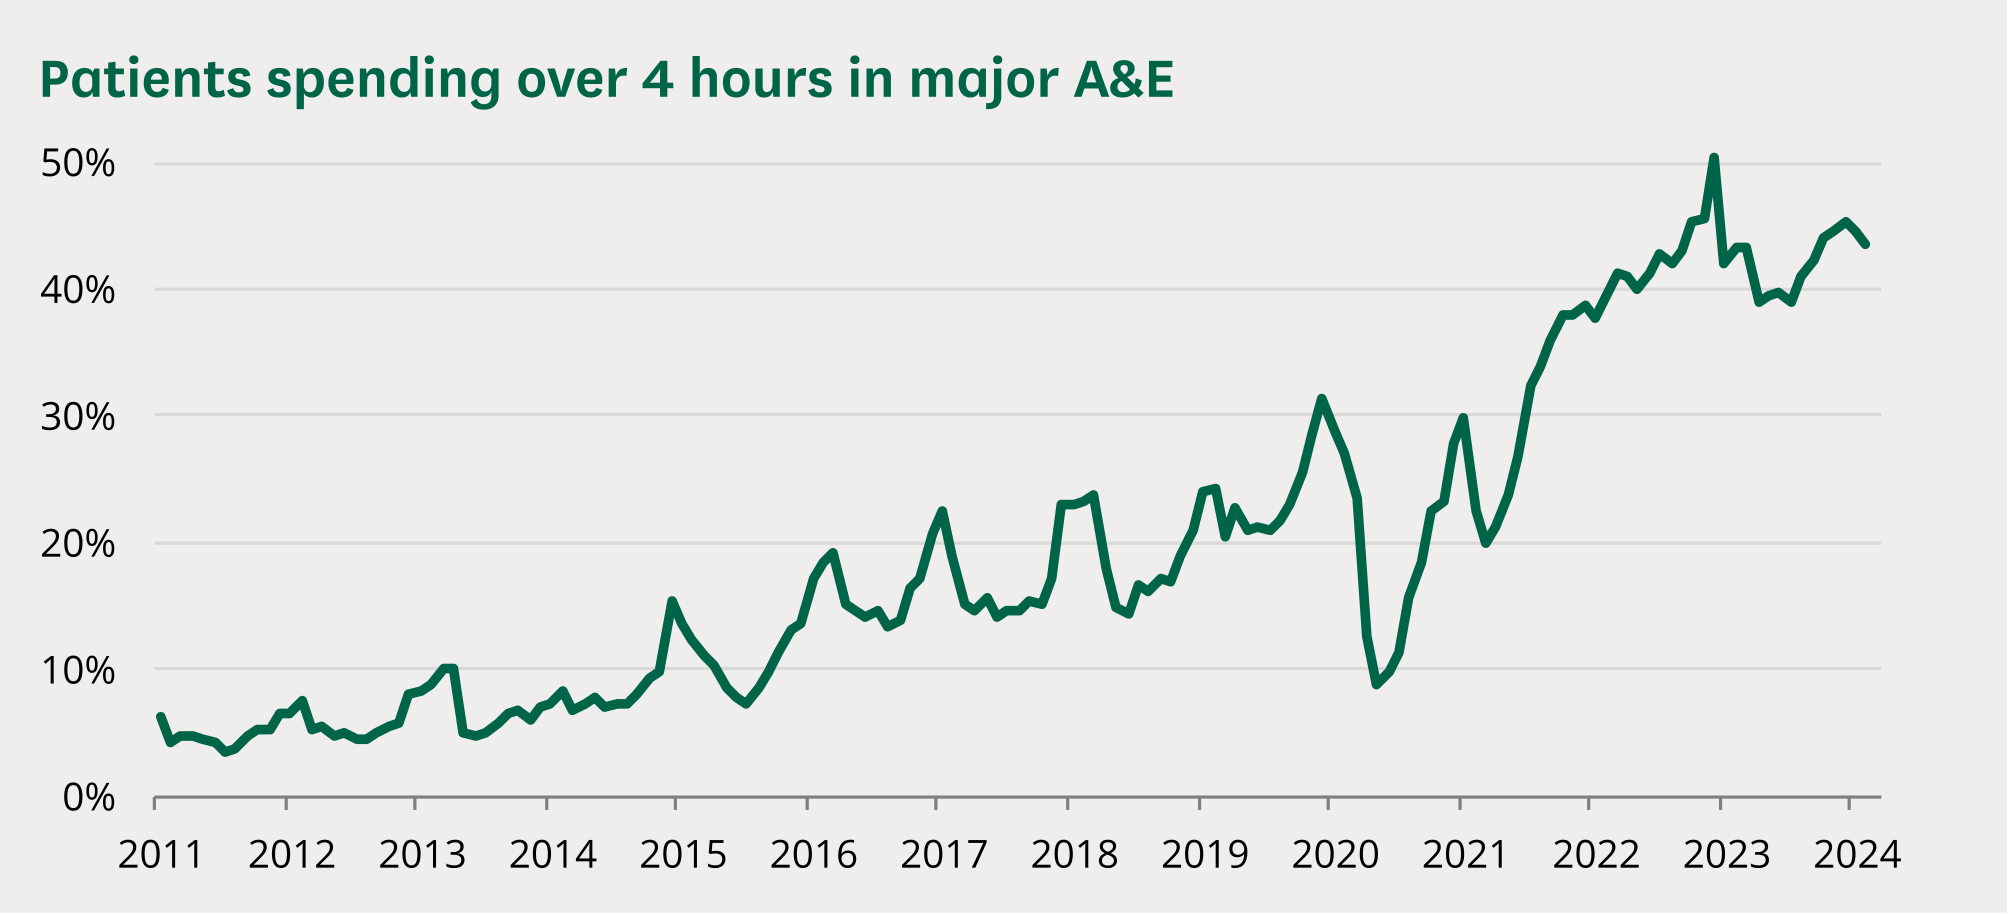
\includegraphics[width=1\linewidth]{img/Figuur-1.png}
    \caption{Percentage van patiënten die meer dan 4 uur spenderen in de Accident and Emergency (A\&E) departement}
    \label{fig:Figuur1}
    \textit{Source: \autocite{Baker2024}}
\end{figure}

Het niet voldoen aan deze richtlijn heeft serieuze gevolgen voor de zorgkwaliteit en patiëntentevredenheid zoals aangetoond door \autocite{Vainieri2020}. Volgens de bevindingen van \autocite{Paling2020} zijn de implicaties veel ernstiger. De studie vermeldt dat lange wachttijden in de Accident and Emergency (A\&E)-afdeling een verband toont met complicaties en mortaliteit onder patiënten. De oorzaak, volgens \autocite{Paling2020}, is te wijten aan een hoge beddenbezettingsgraad. Verder toont het onderzoek een correlatie tussen de hoge beddenbezetting  en de lange wachttijden in de Accident and Emergency (A\&E)-afdeling zoals aangetoond door fig. \ref{fig:Figuur2}.

\begin{figure}[h]
    \centering
    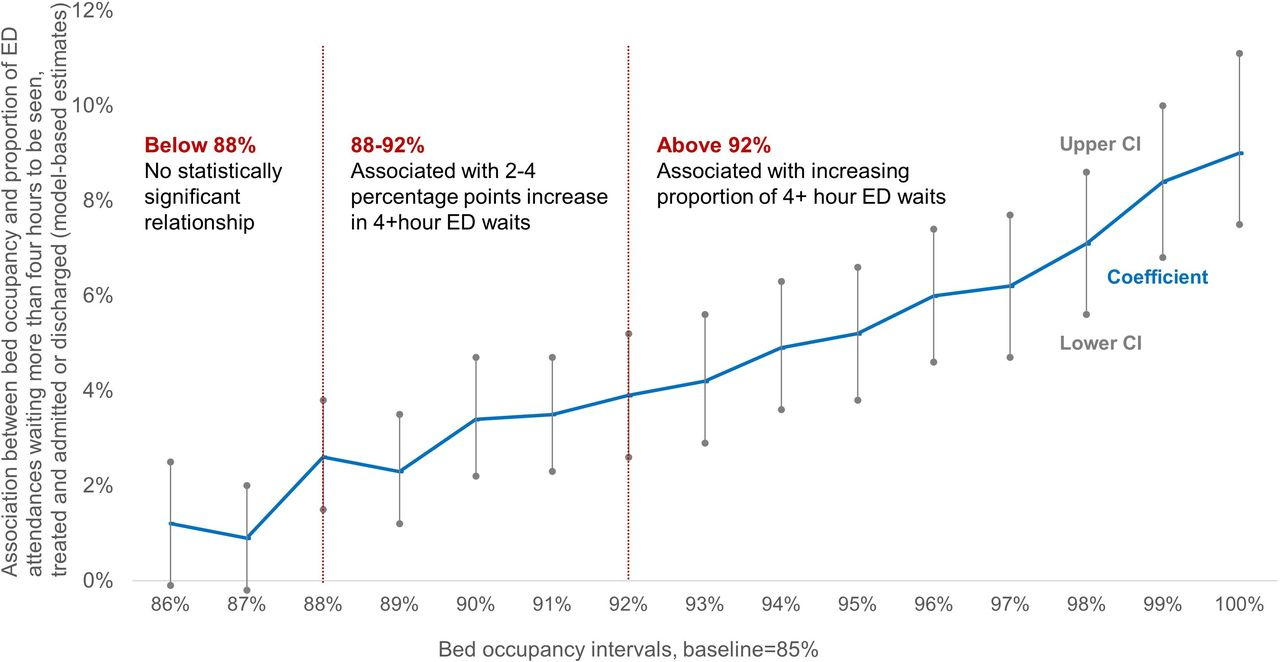
\includegraphics[width=0.5\textwidth]{img/Figuur-2}
    \caption{Plot dat een niet-lineaire relatie toont tussen bedbezettingen intervallen en proportie van patienten die meer dan 4 uur spenderen in de Accident and Emergency (A\&E) departement}
    \label{fig:Figuur2}
    \textit{Source: \autocite{Paling2020}}
\end{figure}

Patiënten zijn niet de enigen die worden beïnvloed door de langdurige wachttijden, onderzoekers hebben onlangs de werkomstandigheden van National Health Service (NHS)-werknemers onderzocht. De studie toont dat 40\% van alle ziektes bij het personeel te wijten is aan stress. Verder wijst het onderzoek uit dat de “overheersende stressfactor” veroorzaakt wordt door de hoge werkdruk \autocite{Ravalier2020}. \autocite{Vainieri2020} onderlijnt overbevolking als oorzaak van de hoge werkbelasting, en dit in Accident and Emergency (A\&E) departementen in diverse westerse landen. Om beter te begrijpen hoe Internet of Things (IoT) dit probleem kan oplossen, is het noodzakelijk om dieper in te gaan op wat Internet of Things (IoT) precies inhoudt. Over het algemeen verwijst Internet of things (IoT) naar een model dat verschillende technologieën omvat. Anders gezegd, is het een netwerk van elektronische apparaten die met elkaar of met de cloud communiceren via het internet. De afgelopen twee decennia hebben een grote invloed gehad op de snelle vooruitgang van Internet of Things (IoT) \autocite{Almutairi2024}, hierdoor is het aantal aangesloten Internet of Things (IoT)-devices sterk gestegen, met 7.74 miljard in 2019, 10.7 miljard in 2021 \autocite{Dawod2022} en 25.44 miljard tegen 2030 \autocite{Dawod2022}. Sensoren, camera's en gelijkaardige apparaten worden al “geïntegreerd” in “woningen” en “voertuigen” \autocite{Dawod2022} en geïmplementeerd over verschillende sectoren zoals de “gezondheidszorg, landbouw, productie” en slimme steden \autocite{Almutairi2024}.

De implementatie van miljarden \autocite{Dawod2022} Internet of Things (IoT)-devices over verschillende sectoren geeft een duidelijk representatie van de veranderingen die Internet of Things (IoT) zal brengen over de manier waarop men leeft, werkt en omgaat met de omgeving \autocite{Almutairi2024}. De vraag is nu of Internet of Things (IoT) gebruikt kan worden in de gezondheidszorg om wachttijden in de Accident \& Emergency departementen te verkorten. Volgens een recente studie uitgevoerd door \autocite{Singh2023} is het perfect mogelijk om Internet of Things (IoT) te implementeren in de gezondheidszorg. Echter, concludeert het onderzoek dat Internet of Things (IoT) een gunstige invloed heeft en dit ondanks de beperkingen in “energie, processing en opslag”. Verder benadrukt de studie dat Internet of Things (IoT) een “veelbelovende technologie” is bij het sparen van tijd en moeite voor het medische personeel. 

%----------------------------------------------------------------------------------------------------------------------

Internet of Things (IoT) kan op verschillende manieren worden ingezet in de gezondheidszorg \autocite{Huang2021}. Ten eerste kan Internet of Things (IoT) toegepast worden voor het beheren van medische uitrusting, medicatie en data. Vervolgens door gebruik te maken van Internet of Things (IoT)-ondersteunende slimme apparaten en systemen kan de patiënten stroom worden beheerd \autocite{Almotaira2023} en patiënten pieken voorspeld \autocite{King2022}. De werking hiervan, zoals aangetoond in fig. \ref{fig:Figuur4} is als volgt, iedere patiënt beschikt over zijn eigen Internet of Things (IoT)-device, zoals een sensor of een netwerk device. De device is vervolgens verbonden met een intelligente gateway, ook wel Internet of Things (IoT)-gateway genoemd. Deze gateway zorgt voor communicatie tussen devices, en tussen device en cloud \autocite{Upadrista2021}. De gateway is verbonden met een datacollectie- en processing center via het internet, deze is verantwoordelijk voor het verwerken van ruwe data door het “correctheid” en “kwaliteit” te verbeteren om deze geschikt voor analyse te maken \autocite{Sirisha2023}. Eenmaal de ruwe data verwerkt, worden deze geanalyseerd en maakt het systeem beslissingen, die vervolgens door artsen en dokters gebruikt kunnen worden \autocite{Singh2023}. Kortom, verzamelen Internet of Things (IoT)-apparaten realtime patiëntgegevens die geanalyseerd zijn om inzichten te maken en trends te voorspellen \autocite{Alrehaili2023, Sidhu2023}. 

\begin{figure}[h]
    \centering
    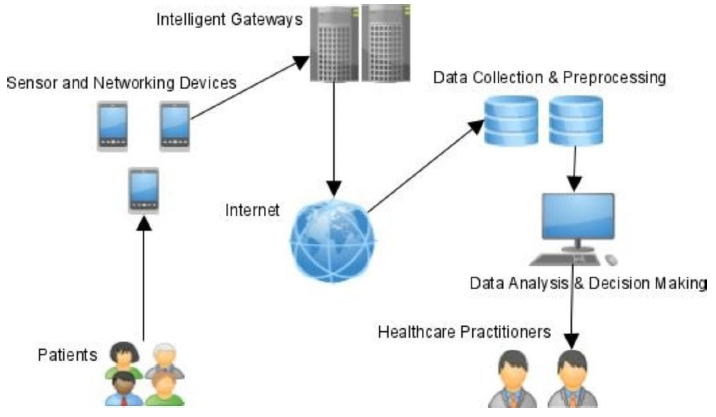
\includegraphics[width=0.5\textwidth]{img/Figuur-4}
    \caption{Internet of things (IoT) systeem in de gezondheidszorg}
    \label{fig:Figuur4}
    \textit{Source: \autocite{Singh2023}}
\end{figure}


%---------- Methodologie ------------------------------------------------------
\section{Methodologie}%
\label{sec:methodologie}

% Hier beschrijf je hoe je van plan bent het onderzoek te voeren. Welke onderzoekstechniek ga je toepassen om elk van je onderzoeksvragen te beantwoorden? Gebruik je hiervoor literatuurstudie, interviews met belanghebbenden (bv.~voor requirements-analyse), experimenten, simulaties, vergelijkende studie, risico-analyse, PoC, \ldots?

% Valt je onderwerp onder één van de typische soorten bachelorproeven die besproken zijn in de lessen Research Methods (bv.\ vergelijkende studie of risico-analyse)? Zorg er dan ook voor dat we duidelijk de verschillende stappen terug vinden die we verwachten in dit soort onderzoek!

% Vermijd onderzoekstechnieken die geen objectieve, meetbare resultaten kunnen opleveren. Enquêtes, bijvoorbeeld, zijn voor een bachelorproef informatica meestal \textbf{niet geschikt}. De antwoorden zijn eerder meningen dan feiten en in de praktijk blijkt het ook bijzonder moeilijk om voldoende respondenten te vinden. Studenten die een enquête willen voeren, hebben meestal ook geen goede definitie van de populatie, waardoor ook niet kan aangetoond worden dat eventuele resultaten representatief zijn.

%Uit dit onderdeel moet duidelijk naar voor komen dat je bachelorproef ook technisch voldoen\-de diepgang zal bevatten. Het zou niet kloppen als een bachelorproef informatica ook door bv.\ een student marketing zou kunnen uitgevoerd worden.

% Je beschrijft ook al welke tools (hardware, software, diensten, \ldots) je denkt hiervoor te gebruiken of te ontwikkelen.

%Probeer ook een tijdschatting te maken. Hoe lang zal je met elke fase van je onderzoek bezig zijn en wat zijn de concrete \emph{deliverables} in elke fase?

Dit onderzoek heeft als doel het verminderen van wachttijden op de Accident and Emergency (A\&E) afdelingen van de National Health Service (NHS) in Engeland door middel van Internet of Things (IoT).


\subsubsection*{Oorzaakanalyse}
Het onderzoek begint met het uitvoeren van een uitgebreide oorzaakanalyse, dit is een fundamentele stap bij het identificeren van de oorzaak van de langdurige wachttijden binnen de A\&E-afdelingen van de National Health Service (NHS). De analyse begint met het definiëren van het probleem, om die reden zal de 5 Whys”-methode toegepast worden samen met een brainstorming-sessie. De 5 Whys”-method is gebruikt om de kern van het probleem te achterhalen en dit door elke keer de vraag waarom te stellen, \ref{fig:Figuur5} en de oorzaak proberen te identificeren via de brainstorming-sessie. Zodra diverse oorzaken geïdentificeerd zijn, begint er een analyse door middel van het Fishbone-model. De reden achter het gebruik van dit model is het voorkomen dat mogelijke onderliggende oorzaken over het hoofd worden gezien. Verder biedt het model simpliciteit bij het trekken van conclusies dankzij een visuele representatie tussen de categorisch weergegeven oorzaken en het probleem. Vervolgens is elke oorzaak zorgvuldig bestudeerd, degene die de grootste impact heeft op langdurige wachttijden is geselecteerd als de hoofdoorzaak. Een overweging is vervolgens gemaakt, om te achterhalen of IoT in het algemeen een oplossing kan zijn voor deze oorzaak. Verder in het onderzoek wordt er dieper bekeken naar welke IoT-devices gebruikt kunnen worden in de gezondheidszorg, zodra de devices geselecteerd zijn, wordt er op een meer diepgaande wijze bekeken hoe de apparaten een oplossing kunnen zijn voor de hoofdoorzaak.

\begin{figure}[h]
    \centering
    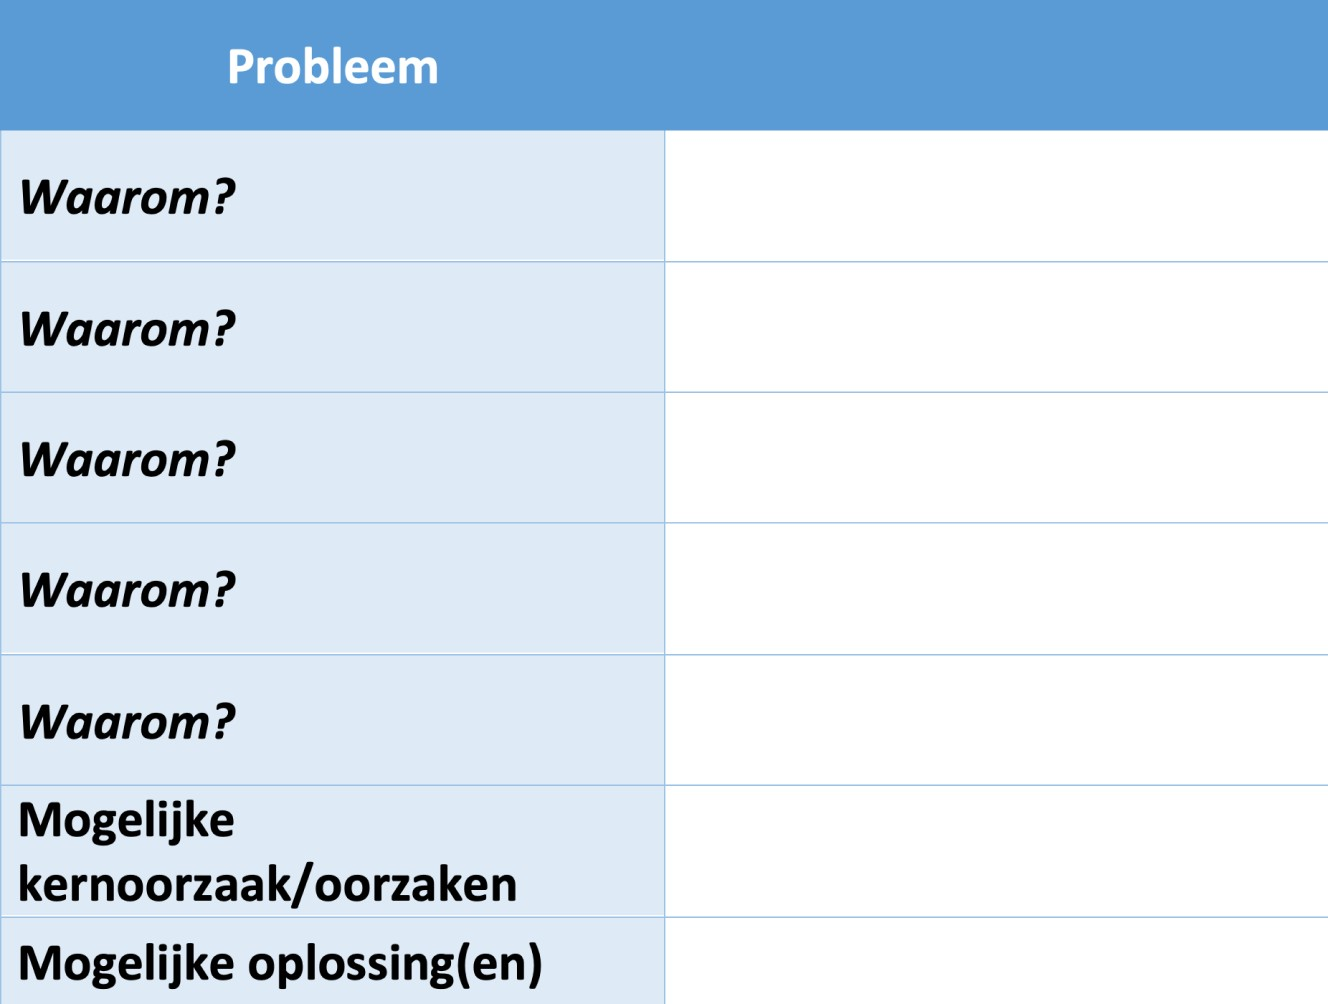
\includegraphics[width=0.5\textwidth]{img/Figuur-5}
    \caption{5 Whys”-method}
    \label{fig:Figuur5}
    \textit{Source: \autocite{Scharwaechter2023}}
\end{figure}

\begin{figure}[h]
    \centering
    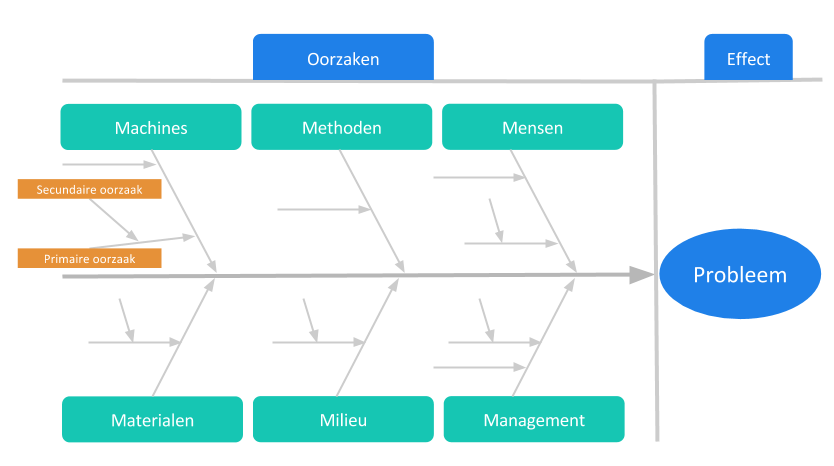
\includegraphics[width=0.5\textwidth]{img/Figuur-6}
    \caption{The fishbone diagram (also called the Ishikawa diagram)}
    \label{fig:Figuur6}
    \textit{Source: \autocite{Swaen2023}}
\end{figure}


%Een oorzaakanalyse is een belangrijk onderdeel van deze onderzoek, voor die reden wordt er een uitgebreide analyse uitgevoerd voor het identificeren oorzaak van de langdurige wachttijden binnen de A\&E-afdelingen van de National Health Service (NHS)

\subsubsection*{Gegevensverzameling}
Het verzamelen van informatie begint met het identificeren van diverse Na-tio-nal Health Ser-vice zie-ken-hui-zen
met de meest uitgebreide wachttijden in de Accident and Emergency (A\&E). Het doel van deze gegevensverzameling is het vaststellen van Na-tio-nal Health Ser-vice zie-ken-hui-zen met uitgebreide Accident and Emergency (A\&E) wachttijden, aangezien deze gegevens essentieel zijn voor de selectieprocedure en simulaties die in de volgende secties aan bod komen. Relevante gegevens worden geselecteerd door verschillende bronnen te raadplegen zoals NHS Digital, NHS UK. De bronnen worden gekozen op basis van hun relevantie voor het onderzoek en datum van publicatie daarvan. Deze datum moet zo recent mogelijk zijn om een representatief beeld te kunnen geven van de huidige toestand, daarvoor zullen enkel gegevens van de laatste maand (maart 2024) behouden worden. De informatie is geselecteerd met als voorwaarde dat deze in CSV-formaat beschikbaar is. Dit formaat maakt het bestand makkelijk aanpasbaar door gebruik te maken van Python wat praktisch is tijdens het verwerken van het bestand. De gegevens dienen ook de naam van de ziekenhuizen te bevatten alsook kwantitatieve gegevens over wachttijden in de Accident and Emergency (A\&E). Dit onderzoek richt zich enkel op ziekenhuizen in Engeland waardoor de namen zeer belangrijk zijn. Als laatste dienen de gegevens een onderscheid te tonen tussen de wachttijden minder dan vier uur en deze meer dan vier wat noodzakelijk is bij het vaststellen van langdurige wachttijden. Na het verzamelen van de nodige gegevens over de National Health Service (NHS)-ziekenhuizen, is het literatuurstudie \ref{sec:literatuurstudie} geraadpleegd voor informatie over de gebruikte Internet of Things (IoT)-devices in Accident and Emergency (A\&E) afdelingen. De verzamelde informatie zal vervolgens gebruikt zijn in de toekomstige simulatie over de gekozen ziekenhuis in de selectieprocedure.

\subsubsection*{Gegevensverwerking en Selectieprocedure}
Python, Numpy en Pandas zijn tools die worden gebruikt voor het verwerken van het dataframe, deze tools zijn gebruikt voor het uitfilteren van de onnodige gegevens. Als eerste wordt de gegevensstructuur geanalyseerd zijn voor het identificeren van de te selecteren kolommen en rijen. Enkel kolommen die gegevens bevatten over het datum en ziekenhuis zijn behouden.

Het dataframe wordt vervolgens gebruikt in de selectieprocedure. Deze procedure houdt in dat een ziekenhuis aan diverse voorwaarden moet voldoen om geselecteerd te zijn, deze criteriums houden in dat een ziekenhuis gelegen moet zijn in Engeland. Verder zijn de ziekenhuizen die nul of geen waarde hebben voor wachttijden over de vier uur niet behouden. het ziekenhuis met de meeste patiënten in de kolom met wachttijden over de 4 uur is geselecteerd.

\subsubsection*{Case study}
Deze case study wordt gerealiseerd als toelichting voor het implementeren van Internet of Things (IoT)-technologieën en dit met als doel om wachttijden in de Accident and Emergency (A\&E) afdelingen van de National Health Service (NHS) te verkorten. De primaire doelstelling van deze case study is het identificeren van praktische voorbeelden van Internet of Things (IoT)-gebruik om lange wachttijden in Accident and Emergency (A\&E)-afdelingen te verminderen. Daarnaast richt de case study zich op het identificeren van verschillende Internet of Things (IoT)-apparaten die ingezet kunnen worden om wachttijden verder te verkorten. De case study begint met het identificeren specifieke casussen. In het geval van deze onderzoeksvraag dienen deze te voldoen aan diverse criteria, deze houden in dat een casus over een bepaald ziekenhuis dient te voldoen aan de criteria, welke zijn vastgesteld in het selectieprocedure, met uitzondering van de locatie. Bovendien dient de gekozen casus, in dit geval één of meerdere ziekenhuizen gebruik maken van Internet of Things (IoT) in Accident and Emergency (A\&E) afdelingen bij het bestrijden van langdurige wachttijden. Na het vast stellen van een casus worden er kwalitatieve en kwantitatieve gegevens verzameld over de gekozen casus, dit houdt in dat verschillende bronnen worden geraadpleegd bij het verzamelen van informatie zoals, wetenschappelijke literatuur, rapporten van gezondheidsorganisaties, archieven en documenten. Een voorbeeld van deze bronnen zijn National Library of Medicine. Na het vaststellen van diverse casussen worden deze vergeleken met het ziekenhuis uit de selectieprocedure, de casus die het meest overeenstemt met de geselecteerde ziekenhuis wordt gekozen. De casus wordt vervolgens geanalyseerd en de gebruikte Internet of Things (IoT)-devices en Internet of Things (IoT)-categorieën opgelijst, verder worden gegevens verzamelt voor elk van de opgelijste devices, verschillende bronnen zoals onderzoeksrapporten, literatuurstudies, academische tijdschriften en technologische onderzoeken worden hiervoor geraadpleegd. De verzamelde gegevens worden vervolgens geanalyseerd met als doel een beter begrip te krijgen over hoe deze in de casus geïmplementeerd zijn en hoe deze toegepast kunnen worden in de geselecteerde ziekenhuis. 


\subsubsection*{Identificeren van IoT-devices}
Het identificeren van IoT-apparaten is van het uiterste belang, daarom is er aanzienlijk veel tijd besteed bij het opstellen van de casestudie om een assortiment van IoT-apparaten te bepalen. Dit houdt in dat elk apparaat grondig bestudeerd zal zijn om een beter begrip te krijgen in de werking hiervan in de gezondheidszorg. Om het meest gepaste IoT-apparaat te selecteren worden verschillende IoT-categorieën bekeken, deze categorieën vertegenwoordigen IoT-apparaten die de werking van de A\&E-departementen kan verbeteren en efficiënter maken, deze categorieën zijn: Locatie- en traceerapparaten, Communicatieapparaten, Geautomatiseerde medicatie dispensers, Integratie van het gegevensbeheer en Integratie en coördinatie van IoT-devices.

De eerste geselecteerde device(s) zijn de RFID-Tags vanuit de Location and Tracking categorie, deze tags zullen ingezet zijn voor het opsporen van patiënten, uitrusting en personeel op de werkvloer, dit IoT-device zorgt ervoor dat alles makkelijk te vinden is, waardoor het personeel zich volledig kan focussen op binnenkomende patiënten.

Verder zullen er Smart Tablets and Displays en Patient Kiosks ingezet zijn, deze behoren tot de categorie Communication Devices, de Smart Tablets and Displays zorgen ervoor dat het personeel in staat zijn om realtime gegevens, waarschuwingen en patiëntinformatie kan ontvangen van patiënten op de spoeddienst. Het gebruik van Smart Tablets and Displays zorgt ervoor dat het personeel steeds beschikt over de meest recente gegevens wat van uiterst belang is bij het verzorgen van patiënten. Daarnaast zullen er Patient Kiosks ingeschakeld zijn, patiënten kunnen deze gebruiken om check-ins of updates te krijgen over de wachttijden en de volgende onderzoeken.

Vervolgens zullen slimme medicijnkastjes en pillendispensers ingeschakeld zijn, de slimme medicijnkastjes zullen gebruikt zijn om het uitgave van medicatie efficiënter te maken dankzij verschillende geautomatiseerde aspecten. Daarnaast zal er een device gebruikt zijn als gecentraliseerde data systeem, of een Central Data Hub, dit IoT-apparaat vereist dat gegevens opgeslagen worden op een centrale locatie, dit zorgt ervoor dat dezelfde patiëntengegevens toegankelijk zijn door het volledige personeel zonder dat de gegevens uit verschillende systemen moeten worden gehaald. Als laatste zal er een IoT Platform samen met een AI and Analytics software ingezet zijn, deze platform is een centrale platform om alle IoT-devices te verbinden, monitoren and beheren, deze zorgt ervoor dat alle devices correct samen werken. De software daarentegen zal gebruikt worden om de data vanuit de IoT-devices te analyseren om vervolgens voorspellingen te maken over de patiëntenstroom en triage benodigdheden.

\subsubsection*{Het gebruik van Machine Learning, Predictive Analytics en synthetische IoT data}
Het complementaire gebruik van Ma\-chi\-ne Lear\-ning, Predictive Analytics en synthetische IoT-\-ge\-ge\-vens is de gekozen methode om te illustreren of Internet of Things (IoT) een gunstig effect heeft op het terugdringen van lange wachttijden voor de National Health Service (NHS). Deze keuze is gemaakt vanwege de vele uitdagingen om dit in de werkelijkheid te testen. Kortom, zijn er nog veel drempels bij het uitvoeren van gelijkaardige testen, vooral in National Health Service (NHS)-ziekenhuizen. Daardoor wordt er gekozen om gebruik te maken van Machine Learning, Predictive Analytics en synthetische IoT-gegevens om aan te tonen dat IoT een gunstige invloed heeft bij het verkorten van langdurige wachttijden. Om dit doel te vervullen zijn de Machine Learning en Predictive Analytics algoritmes eerst en vooral getraind, en dit door middel van verzamelde historische gegevens en synthetische IoT data. Verder volgt er de generatie van de synthetische IoT data voor elk IoT device door middel van Python en Python libraries zoals Pandas, Numpy en Faker. De synthetische data bevat gegevens over de diverse verplaatsingen van patiënten binnen de A\&E en de tijd die op elke locatie doorgebracht zijn. Eenmaal de algoritmes getraind kan het model gebruikt worden om wachttijden te voorspellen tijdens de patiëntenflow \ref{fig:Figuur6} voor diverse scenario's zoals veranderingen in het aantal patiënten en personeel. Tot slot worden de wachttijden voor de diverse scenario's vergeleken met de historische data en worden er conclusies getrokken en de onderzoeksvraag beantwoord.

\begin{figure}[h]
    \centering
    \includegraphics[width=0.5\textwidth]{img/Figuur-7}
    \caption{Patiëntenflow A\&E}
    \label{fig:Figuur7}
    \textit{Source: \autocite{Morris}}
\end{figure}

\subsubsection*{Resultaten}

De resultaten worden beschouwd als een succes, indien de voorspellingen duidelijk aan tonen dat er een significant vermindering is in de wachttijden na het gebruik van Internet of Things (IoT). Dit gebeurt door de voorspellingen te vergelijken met de historische data, hieruit worden conclusies getrokken

De bevindingen met betrekking tot de voorspellingen worden vergeleken met de historische data, de waarnemingen die daaruit volgen worden vervolgens geanalyseerd in de context van potentiële voordelen van Internet of Things (IoT) met betrekking tot de uitgebreide Accident and Emergency (A\&E) wachttijden. De resultaten van het onderzoek lichten verder toe of Internet of Things (IoT) kan bijdragen bij het verminderen van wachttijden voor de Accident and Emergency (A\&E) afdeling door gebruik te maken van technologieën uit verschillende IoT categorieën. Als er voldoende aanwijzingen zijn dat Internet of Things (IoT)-tech\-no\-lo\-gieën een gunstige invloed hebben op de wachttijden binnen de Accident and Emergency (A\&E) afdeling, dan zijn de resultaten als succesvol gewaardeerd.


\subsubsection*{Milestone}

\begin{figure}[h]
    \centering
    \includegraphics[width=0.93\linewidth]{img/milestone-2.png}
    \label{fig:Figuur8}
\end{figure} 

%---------- Verwachte resultaten ----------------------------------------------
\section{Verwacht resultaat, conclusie}%
\label{sec:verwachte_resultaten}

Hier beschrijf je welke resultaten je verwacht. Als je metingen en simulaties uitvoert, kan je hier al mock-ups maken van de grafieken samen met de verwachte conclusies. Benoem zeker al je assen en de onderdelen van de grafiek die je gaat gebruiken. Dit zorgt ervoor dat je concreet weet welk soort data je moet verzamelen en hoe je die moet meten.

Wat heeft de doelgroep van je onderzoek aan het resultaat? Op welke manier zorgt jouw bachelorproef voor een meerwaarde?

Hier beschrijf je wat je verwacht uit je onderzoek, met de motivatie waarom. Het is \textbf{niet} erg indien uit je onderzoek andere resultaten en conclusies vloeien dan dat je hier beschrijft: het is dan juist interessant om te onderzoeken waarom jouw hypothesen niet overeenkomen met de resultaten.



%%---------- Andere bijlagen --------------------------------------------------
% TODO: Voeg hier eventuele andere bijlagen toe. Bv. als je deze BP voor de
% tweede keer indient, een overzicht van de verbeteringen t.o.v. het origineel.
%\input{...}

%%---------- Backmatter, referentielijst ---------------------------------------

\backmatter{}

\setlength\bibitemsep{2pt} %% Add Some space between the bibliograpy entries
\printbibliography[heading=bibintoc]

\end{document}
